\RequirePackage{snapshot}
\documentclass[a4paper,twoside]{alpenthesis/alpenthesis}
% ==============================================================================
%
%                               P R E A M B L E
%
% ==============================================================================
% <<< ----------------------------------------------------------------PREAMBLE %
\hextrue
%\aiiistock % Compile twice for A4, then once for A3, with hextrue
\papertrue
%https://tex.stackexchange.com/a/210456/131649
\renewcommand\partnumberlinebox[2]{#2\hspace{2em}}
\ifpaper
    \hypersetup{%
        linkcolor=black,
        citecolor=black,
        urlcolor=black,%
    }
\fi
\usetikzlibrary{positioning}
\usetikzlibrary{spy}
\usetikzlibrary{fit}
\usepackage{multirow,array}
\tcbuselibrary{breakable}
\tcbset{shield externalize}
\usepgfplotslibrary{fillbetween}
\usepgfplotslibrary{units}
\usepgfplotslibrary{groupplots}
\usepackage{pgfplotstable}
\DeclareSIUnit\sample{sample}
\DeclareSIUnit\channel{channel}
\DeclareSIUnit[number-unit-product = {}]\partspermillion{ppm}
\DeclareSIUnit[number-unit-product = {}]\permille{\perthousand}
\usepackage[simplified]{pgf-umlcd}
\usepackage{algorithmicx}
\usepackage{algpseudocode}
\usepackage{algorithm}
\usepackage{pdfpages}
\usepackage{dirtree}
\pgfplotsset{
    %title style={font=\bfseries\sffamily\mathversion{boldsf}},
    every axis title/.style={
        font=\sffamily\mathversion{sf},
        at={(0.5,1)},above,yshift=1pt
    },
    xlabel near ticks=true,
    ylabel near ticks=true,
    xticklabel style={font=\footnotesize},
    yticklabel style={font=\footnotesize},
    xlabel style={font=\footnotesize},
    ylabel style={font=\footnotesize},
    scale only axis,
    every axis legend/.append style={
        font=\footnotesize,
    },
    every x tick scale label/.style={
        at={(1.0,0)},
        xshift=1pt,
        anchor=south west,
        inner sep=2pt
    },
}
\makeindex
%\includeonly{chunks/introduction,chunks/theory}
% >>>
\begin{document}

% ==============================================================================
%
%                            T I T L I N G P A G E
%
% ==============================================================================
% <<< ------------------------------------------------------------ TITLINGPAGE %
\begin{titlingpage}
    \fullhexpage{q1}{q0}
    \flushright\sffamily
    \enlargethispage{10ex}

    \vspace*{5em}
    
    \Huge\bfseries{Front-End Signal Processing for Red Pitaya Spectrum Analyzer}\\[1ex]
    \Large\mdseries{Bachelor Thesis}\\[3ex]

    \normalsize\mdseries

    \tikzexternaldisable
%\tikzsetnextfilename{titlepage}
\begin{tikzpicture}[
    signalPath/.style={
        draw=q4,,
        fill=q4!50!white,
        circle,
        inner sep=0.3mm,
    },
    remember picture,
    overlay,
]
     \pgfplotsset{
         every axis/.style={
            anchor=center,
            at={(current page.center)},
            width=165mm,
            height=100mm,
            grid=none,
            axis line style={draw=none},
            tick style={draw=none},
            ticks = none,
            each nth point=4,
            filter discard warning=false,
            unbounded coords=discard,
            yshift=-6.75mm,
            xshift=16mm,
        }
    }
    \begin{axis}
        \addplot[ycomb,mark=*,mark options={scale=0.75},very thin,q1] 
            table[x=t,y=h,col sep=comma] {images/titlepage/impzChain25.csv};
    \end{axis}
\end{tikzpicture}
\tikzexternalenable


    \vfill
    \begin{tabular}{>{\bfseries}rl}
        Degree Program: & Electrical Engineering and Information Technology \\[2mm]
        Course:         & Project \num{6}\\[2mm]
        Coaches:        & Prof. Dr. Richard Gut, Michael Pichler \\[2mm]
        External Expert & Dr. J\"urg Stettbacher \\[2mm]
        Team:           & Raphael Frey, Noah H\"usser \\[2mm]
        Date:           & August 18, 2017 \\[2mm]
        Revision:       & 1.0.0 \\[2mm]
    \end{tabular}

    \tikzexternaldisable
        \begin{tikzpicture}[remember picture,overlay]
            \node[anchor=north east,yshift=-2.5mm,xshift=-2.5mm,] 
                at (current page.north east) {
\includegraphics[width=10cm]{images/titlepage/logo-fhnw.pdf}};
            \node[anchor=south east,yshift=2.5mm,xshift=-2.5mm,] 
                at (current page.south east) {
\includegraphics[width=4cm]{images/titlepage/logo-ime.pdf}};
        \end{tikzpicture}
    \tikzexternalenable
\end{titlingpage} % >>>
% ==============================================================================
%
%                            F R O N T M A T T E R
%
% ==============================================================================
%<<< ------------------------------------------------------------ FRONT MATTER %
\frontmatter
% <<< --------------------------------------------------------------- ABSTRACT %
% ==============================================================================
%
%                               A B S T R A C T
%
% ==============================================================================
\chapter*{Abstract} % -------------------------------------------------------- %
\label{ch:app:abstract}
% ---------------------------------------------------------------------------- %

The objective  of this  project is  to realize a  system for  measuring analog
signals  in  the kilohertz  to  low  megahertz  range  with a  digital  signal
processing  system  in  real  time,  offering  an  affordable  alternative  to
expensive oscilloscopes  and spectrum  analyzers. The basic components  of the
system are a  Red Pitaya STEMlab for signal acquisition  and processing  and a
personal  computer  or  mobile  device  for  data  visualization  and  further
analysis.

To  allow transmission  over  an  Ethernet connection  and  to improve  signal
quality, the high-rate data stream coming from the STEMlab's analog-to-digital
converter  is   decimated  to  a   lower-rate  signal  using   the  integrated
FPGA. During decimation, the signal passes through one of six filter chains to
attenuate aliasing  effects. 

The chains  run on  the STEMlab's  FPGA. They are based  on a  combination of
FIR  and CIC  filters,  and  decimate the  incoming  \SI{125}{\MHz} signal  to
output frequencies  between \SI{50}{\kHz} and \SI{25}{\MHz},  depending on the
chain. They  achieve  an  aliasing  attenuation of  \SI{60}{\dB}  and  exhibit
negligible passband droop. A  signal-to-noise ratio of up  to \SI{84}{\dB} has
been measured.

The decimated signal is then passed on  to an embedded GNU/Linux and sent to a
client over  a network connection. A newly  developed oscilloscope application
allows observation  of the signal  from a  client device.  The  application is
based on JavaScript,  allowing for easy deployment across any  platform with a
modern browser available.

All components created for this project  are provided under the MIT license. A
comprehensive toolchain covering filter design, FPGA tools, embedded GNU/Linux
and front end  development, along with documentation, allows  anyone to extend
and modify the system and to tailor it to their needs.

\vfill

%<<< KEYWORDS
\paragraph{Key Words:} 
Red Pitaya,
STEMlab,
Xilinx,
FPGA,
Oscilloscope,
Spectrum Analyzer,
DSP,
digital signal processing,
digital filters,
FIR Filter,
CIC Filter,
lowpass,
sampling,
downsampling,
decimation,
aliasing,
attenuation,
FFT,
JavaScript,
web application,
VHDL,
C,
C++,
open source,
MIT license.
%>>> KEYWORDS
%^^A vim: foldenable foldcolumn=4 foldmethod=marker foldmarker=<<<,>>>

% >>> ABSTRACT
% <<< ----------------------------------------------------------------- THANKS %
% ==============================================================================
%
%                                 T H A N K S
%
% ==============================================================================
\chapter*{Thanks} % ---------------------------------------------------------- %
\label{ch:app:thanks}
% ---------------------------------------------------------------------------- %
\vspace{16em}

Many thanks go  to all the people  who have supported us  during our studies,
and this project in particular:

\begin{itemize}
    \item[]\emph{Friends and families}, for their patience when we were absent
        from their lives.
    \item[]\emph{Richard Gut}, for showing  much patience in explaining things
        again  and again  when our  minds proved  resistant to  digital signal
        processing insight.
    \item[]\emph{Michael Pichler}, for his support when debuggin FPGA problems.
    \item[]\emph{Hanspeter Schmid}, for his help with understanding the magic
        of CIC filters and SNR calculations.
    \item[]\emph{Hans Buchmann},  for his  avid enthusiasm  in helping  us to
        figure out device trees on GNU/Linux.
    \item[]\emph{Pavel Demin}, for his ADC core and prompt technical support
        in helping us to understand the innards of the STEMlab.
\end{itemize}

%^^A vim: foldenable foldcolumn=4 foldmethod=marker foldmarker=<<<,>>>

% >>> THANKS
% <<< -------------------------------------------------------- ToC AND FRIENDS %
% https://en.wikipedia.org/wiki/Edition_notice
\renewcommand*\contentsname{Short Contents}
\setcounter{tocdepth}{0}
\tableofcontents*
\renewcommand*\contentsname{Contents}
\setcounter{tocdepth}{3}
\cleardoublepage
\tableofcontents*
\clearpage
\listoffigures*
\clearpage
\listoftables*
\clearpage
\listoflistings
\clearpage
% >>> ToC AND FRIENDS
% >>> FRONT MATTER
% ==============================================================================
%
%                             M A I N M A T T E R
%
% ==============================================================================
\mainmatter
% ==============================================================================
%
%                           I N T R O D U C T I O N
%
% ==============================================================================
% <<< ----------------------------------------------------------- INTRODUCTION %
% ==============================================================================
%
%                           I N T R O D U C T I O N
%
% ==============================================================================
\chapter*{Introduction} % ---------------------------------------------------- %
\label{ch:intro}
\addcontentsline{toc}{chapter}{\nameref{ch:intro}}
% ---------------------------------------------------------------------------- %

Electronic measuring equipment has historically tended to be very pricey, with
specialized appliances  sometimes costing  as much as  a middle-class  car, or
even more. While high-performance  solutions are unlikely to  be replaced with
something radically  different in  the foreseeable future,  modern, affordable
FPGAs  are  a  viable  alternative  in many  use  cases  nowadays. By  keeping
performance requirements within reasonable bounds and pairing the FPGA with an
appropriate  front-end, sufficient  performance for  many applications  can be
achieved  at a  very competitive  price point.   Additionally, an  FPGA offers
vastly  superior flexibility  over the  fixed silicon  of conventional  signal
processing chips,  since its hardware  capabilities can be altered  even after
deployment.

A suitable front-end for an FPGA usually comprises dedicated ADCs and DACs and
analog  filters. Along with  FPGA chips  themselves,  ADC and  DAC chips  have
become much more economical in recent  years, resulting in a product which may
cost  as little  as  a few  hundred  Swiss  Francs and  which  can replace  an
apparatus several times as expensive.

This project  aims to  equip such an  FPGA board with  logic that  can record,
filter  and store  electrical signals  with  adjustable sampling  rates up  to
\SI{125}{\mega\hertz}.   To  complement  the hardware  subsystem,  a  software
component is provided, consisting of two applications: One runs on an embedded
GNU/Linux on the board itself, while  the other runs on a user's computer. The
application on the  board (the \emph{server}) is  responsible for transmitting
the recorded data over a network connection, while the software running on the
user's  computer  (the oscilloscope,  or  \emph{scope}  for short)  serves  to
visualize and  process the  measurement results. This  concept is  depicted in
Figure~\ref{fig:intro:system_overview}.

\makeatletter
\renewcommand{\thefigure}{\@arabic\c@figure}
\makeatother
\begin{figure}
    \centering
    \tikzsetnextfilename{intro-system-overview}
\begin{tikzpicture}[
    rounded corners=1mm,
    node distance=5mm,
    fpgaComponent/.style={
        draw,
        minimum height=12ex,
        fill=q4,
    },
    SoCComponent/.style={
        minimum height=8ex,
        minimum width=6em,
        fill=ct2,
        draw=sqC,
        text=br2,
        font=\bfseries,
    },
]
    \small
    \sffamily

    \node[SoCComponent] at (0,0) (fpga) {FPGA};
    \node[SoCComponent,right=of fpga] (server) {Server};

    \begin{scope}[on background layer]
        \node[
            draw=black,
            fit=(fpga) (server),
            inner sep=2mm,
            align=left,
            text height=11ex,
            minimum height=16ex,
            fill=br1,
            text=black,
            font=\bfseries,
        ] (board) {Board};
    \end{scope}

    \node[
        right=10mm of board,
        minimum width=12ex,
        minimum height=8ex,
        fill=ct2,
        align=center,
        text=br2,
    ] (pcmonitor) {\bfseries Scope\\\\};

    \begin{scope}[on background layer]
        \node[
            draw=black,
            fit=(pcmonitor),
            minimum height=8ex,
            fill=black!60!white,
        ] (pcmonitorframe) {};
    \end{scope}

    \fill[br2] ($(pcmonitorframe.south) + (-1ex,0)$) --+ (0,-1ex) --+ (2ex,-1ex) --+ (2ex,0) -- cycle;
    \draw ($(pcmonitorframe.south) + (-1ex,0)$) --+ (0,-1ex);
    \draw ($(pcmonitorframe.south) + (1ex,0)$)--+ (0,-1ex);
    \draw ($(pcmonitorframe.south) + (1ex,0)$)--+ (0,-1ex);
    \draw[fill=br2] ($(pcmonitorframe.south) + (-6ex,-1ex)$) rectangle
          ($(pcmonitorframe.south) + (+6ex,-3ex)$);

    \draw[thick,-latex] (-18.0mm,0mm) -- ($(board.west) + (-1mm,0mm)$);
    \draw[thick,-latex] ($(board.east) + (1mm,0mm)$) -- ($(pcmonitorframe.west) + (-1mm,0mm)$);
    \draw[thick,-latex] ($(fpga.east) + (0.5mm,0mm)$) -- ($(server.west) + (-0.5mm,0mm)$);

    \begin{axis}[
        anchor=east,
        at={(-20mm,0mm)},
        width=20mm,
        height=10mm,
        axis line style={draw=none},
        tick style={draw=none},
        grid=none,
        ticks = none,
        xmin=0,
        xmax=360,
        ymin=-1.1,
        ymax=1.1,
        samples=500,
    ]
        \addplot[line cap=round,very thick,q1,domain=0:360,-]{sin(x)};
    \end{axis}

    \begin{axis}[
        anchor=south,
        yshift=1mm,
        at={(pcmonitor.south)},
        width=12mm,
        height=6mm,
        axis line style={draw=none},
        tick style={draw=none},
        grid=none,
        ticks = none,
        xmin=0,
        xmax=360,
        ymin=-1.3,
        ymax=1.3,
        samples=500,
    ]
        \addplot[very thick,q4,domain=0:360]{sin(x)};
    \end{axis}

    \node[font=\bfseries\footnotesize,text=black] at (-29mm,-8.95mm) {Signal};
\end{tikzpicture}

    \caption[System Overview]{%
        An overview of the main system components.  An analog signal (left) is
        measured, the data  goes into the server  and is  then transmitted via
        network to a computer running the scope.%
    }
    \label{fig:intro:system_overview}
\end{figure}
\makeatletter
\renewcommand{\thefigure}{\thechapter.\@arabic\c@figure}
\makeatother

The  objective  of  this  project  is   to  provide  a  device  which  enables
students and hobbyists  to analyze signals encompassing the  region from audio
frequencies  to the  low megahertz  range. Compared to  the frequencies  which
modern hardware  can handle  (dozens to hundreds  of megahertz),  the sampling
rates required to process such signals  can be kept within the limits suitable
for an FPGA.

A RedPitaya  STEMlab 125-14 board  is used as  the basis for  the hardware. It
easily offers  sufficient performance  to process the  signals in  the desired
range, having an  ADC which provides a \SI{14}{\bit}  signal at \SI{125}{\MHz}
on two channels.   Indeed, downsampling this signal is  \emph{necessary} if it
is  to be  transmitted over  a  network connection,  since its  data rate  far
exceeds the available bandwidth.

Thus, two primary objectives can be defined:
\begin{enumerate}\tightlist
    \item
        The signal coming out of the ADC must be decimated.
    \item
        The resulting data stream must be visualized for the end user.
\end{enumerate}

Downsampling the  data provided by the  ADC is performed on  the FPGA. Because
downsampling introduces  unwanted frequencies  into the signal's  spectrum, it
needs  to be  processed  by filters  which  attenuate those  components. While
the  STEMlab  offers  some  limited  capability in  this  area  in  its  stock
configuration,  this was  deemed insufficient  and has  been improved  in this
project. Several  filter  chains are  implemented  to  allow decimation  rates
between \num{5}  and \num{2500},  corresponding to output  frequencies between
\SI{25}{\MHz}  and \SI{50}{\kHz},  respectively. The  server application  then
transmits the filtered data stream over Ethernet to a client.

The filter chains have achieved a  signal-to-noise ratio of up to \SI{84}{\dB}
in tests,  depending on  the chosen  chain and  input frequency. Additionally,
the  \SI{14}{\bit}  signal from  the  ADC  is  improved by  \SI{1.2}{\bit}  to
\SI{1.8}{\bit}, again depending on  the chain. Passband shapes show negligible
droop, and stopband aliasing is \SI{60}{\dB}.

Cost-effective FPGA  boards like the  STEMlab usually come without  a physical
user interface  with displays and  buttons. This keeps the device  compact and
its cost  low.  Since fast  personal computers  are ubiquitous these  days, it
seems obvious  to exploit that and  run an oscilloscope application  on such a
device. Due to  the fragmentation of  the modern computing world  into various
ecosystems (Windows, GNU/Linux, macOS, Android, \ldots), web technologies form
the foundation of  the scope; the application can be  accessed from any modern
browser. This makes life easier both for the developers and for the end users.

\paragraph{This      document      is      split      into      four      main
parts:} Part~\ref{part:project_report},    contains   the    primary   project
report. Part~\ref{part:Developer_Guide}   is   the    developer   guide,   and
begins   on  page~\pageref{part:Developer_Guide}. A   short   user  guide   is
provided  in  Part~\ref{part:User_Guide}  from  page~\pageref{part:User_Guide}
onwards. Appendices   are   located   on   page~\pageref{ch:app:fdesign}   and
onwards.
%Depending  on  the  report version,  Appendix~\ref{ch:app:media}  may
%contain a copy of the project repository.

The   project  report   covers  information   relevant  to   the  design   and
implementation of the final product. Its first chapter starts on presents some
relevant theoretical background on digital signal processing, with an emphasis
on digital  filtes  and CIC  filters in particular. The next  chapter outlines
the  process leading  to  the concept  for  our product,  and  compares a  few
alternative choices against it, beginning on page~\pageref{ch:mission}.

The    design   and    implementation    of   the    product   is    detailled
in     Chapters~\ref{ch:filter_design},     \ref{ch:fpga},     \ref{ch:server}
and~\ref{ch:graphical_front_end}. Chapter~\ref{ch:filter_design} documents the
filter  design;  both  requirements   and  specifications  are  documented. An
overview  of  the  FPGA  implementation  is  given  in  Chapter~\ref{ch:fpga},
highlighting some key points  which proved challenging during development. The
transmission   of   data   between   STEMlab  and   client   is   handled   by
a   server   application,  documented   in   Chapter~\ref{ch:server}. Finally,
the    concepts   and    design   choices    underpinning   the    scope   are
explained   in    Chapter~\ref{ch:graphical_front_end}. The   chapters   begin
on  pages~\pageref{ch:filter_design},  \pageref{ch:fpga},  \pageref{ch:server}
and~\pageref{ch:graphical_front_end}, respectively.

The  product's  performance  is assessed  in  \emph{\nameref{ch:verification}}
from page~\pageref{ch:verification}  onwards, and Chapter~\ref{ch:conclusions}
contains some  concluding remarks  on the overall  result and  possible future
steps.

The Developer and  User Guides are mostly  self-contained. The Developer Guide
is  intended for  people who  wish to  use  our product,  or parts  of it,  to
implement a system of their own. The  User Guide is intended for end-users who
wish to perform measurements with our product.

\enlargethispage{6ex}
\vspace{1ex}
\noindent All  components specifically developed  for this project  fall under
the MIT license, a copy of which is located in Appendix~\ref{ch:app:licenses}.

%^^A vim: foldenable foldcolumn=4 foldmethod=marker foldmarker=<<<,>>>

% ------------------------------------------------------------------------->>> %
% ==============================================================================
%
%                         P R O J E C T   R E P O R T
%
% ==============================================================================
% <<< --------------------------------------------------- PART: PROJECT REPORT %
\part{Project Report}
\label{part:project_report}
% ---------------------------------------------------------------------------- %
% <<< ----------------------------------------------------------------- THEORY %
% ==============================================================================
%
%                 T H E O R E T I C A L   B A C K G R O U N D
%
% ==============================================================================
\chapter{Theoretical Background} % ------------------------------------------- %
\label{ch:theory}
% ---------------------------------------------------------------------------- %
% ==============================================================================
%
%                               O V E R V I E W
%
% ==============================================================================

This  chapter presents  a  brief  synopsis on  some  aspects  of digital  data
acquisition from  an analog source  and the processing  of that data,  and how
those issues pertain to our project. It  is not intended to be a comprehensive
treatise on the subject but shall serve  as a short refresher. At its end, the
reader should  have sufficient insight  to understand the basic  motivation of
our project from a theoretical point of view.

% ==============================================================================
%
%                              D S P   C H A I N
%
% ==============================================================================
\section{The Digital Signal Processing Chain}% <<< --------------------------- %
\label{sec:dsp_chain}
% ---------------------------------------------------------------------------- %

Digitally acquiring a signal generally requires at least the following steps:
\begin{itemize}\tightlist
        \item
            Passing the signal through an analog low-pass filter.
        \item
            Sampling and quantizing the filtered signal.
\end{itemize}

The   resulting   sequence  of   values   can   then  be   further   digitally
processed. The necessary  building blocks  for this  process are  portrayed in
Figure~\ref{fig:dspChain:blocks}.

\begin{figure}
    \centering
    \tikzsetnextfilename{dspChain}
\begin{tikzpicture}[
    dspBlock/.style={
        draw=sqC,
        rounded corners=1mm,
        fill=sq3,
        minimum height=3.5ex,
        minimum width=4em,
    },
    signalPath/.style={
        draw=q4,,
        fill=q4!50!white,
        circle,
        inner sep=0.3mm,
    }
]
    \coordinate (in) at (-1.5,0);
    \coordinate (out) at (7.5,0);

    \node[dspBlock] (LP)  at (0,0) {LP};
    \node[dspBlock] (ADC) at (3,0) {ADC};
    \node[dspBlock] (DSP) at (6,0) {DSP};

    \draw[-latex] (in)  -- (LP);
    \draw[-latex] (LP)  -- (ADC);
    \draw[-latex] (ADC) -- (DSP);
    \draw[-latex] (DSP) -- (out);

    \node[above      =1ex] (a1a) at (in)       {A};
    \node[above right=1ex] (a2a) at (LP.east)  {A};
    \node[above right=1ex] (d1a) at (ADC.east) {D};
    \node[above      =1ex] (d2a) at (out)      {D};

    \node[signalPath,below=4ex] (a1b) at (a1a) {\footnotesize 1};
    \node[signalPath,below=4ex] (a2b) at (a2a) {\footnotesize 2};
    \node[signalPath,below=4ex] (d1b) at (d1a) {\footnotesize 3};
\end{tikzpicture}

    \caption[The DSP Chain]{%
        The  basic  building   blocks  of  the  DSP  chain   from  its  analog
        input  to its  digitally processed  output.  From  left to  right: The
        analog  low-pass filter  (\emph{LP}), the  analog-to-digital converter
        (\emph{ADC}), and  an arbitrary  digital signal processing  system for
        further processing of the ADC's output (\emph{DSP}).%
    }
    \label{fig:dspChain:blocks}
\end{figure}

\begin{figure}
    \centering
    \tikzsetnextfilename{dspChainTimeDomain}
\begin{tikzpicture}[
    signalPath/.style={
        draw=q4,,
        fill=q4!50!white,
        circle,
        inner sep=0.3mm,
    }
]
     \pgfplotsset{every axis/.style={
            width=30mm,
            height=25mm,
            grid=none,
            axis line style={draw=none},
            tick style={draw=none},
            ticks = none,
        }
    }
    \begin{axis}[
        at = {(0,0)},
    ]
        \addplot[thick,q1,-] 
            table[x=t,y=y,col sep=comma] {images/dspChain/noisySine.csv};
    \end{axis}

    \begin{axis}[
        at = {(40mm,0)},
    ]
        \addplot[thick,q1,-,smooth] 
            table[x=t,y=y,col sep=comma] {images/dspChain/smoothSine.csv};
    \end{axis}

    \begin{axis}[
        at = {(80mm,0)},
    ]
        \addplot[q1,ycomb,mark=o,mark size=1.0]
            table[x=t,y=y,col sep=comma] {images/dspChain/sampledSine.csv};
    \end{axis}
    \draw[-latex] (2.9,1.25) -- (3.95,1.25);
    \draw[-latex] (6.9,1.25) -- (7.95,1.25);

    \node[signalPath] at (1.50,2.75) {\footnotesize 1};
    \node[signalPath] at (5.50,2.75) {\footnotesize 2};
    \node[signalPath] at (9.50,2.75) {\footnotesize 3};
\end{tikzpicture}

    \begin{tikzpicture}
     \pgfplotsset{every axis/.style={
            height=30mm,
            width=40mm,
            grid=none,
            axis line style={draw=none},
            tick style={draw=none},
            ticks = none,
        }
    }
    \begin{axis}[
        at = {(0,0)},
    ]
        \addplot[-] table[x=t,y=y,col sep=comma] {images/dspChain/spectrumFlat.csv};
    \end{axis}

    \begin{axis}[
        at = {(40mm,0)},
    ]
        \addplot[-,smooth] table[x=t,y=y,col sep=comma] {images/dspChain/spectrumLP.csv};
    \end{axis}

    \begin{axis}[
        at = {(80mm,0)},
    ]
        \addplot[-,smooth] table[x=t,y=y,col sep=comma] {images/dspChain/spectrumSampled.csv};
    \end{axis}
    \draw[-latex] (2.5,0.75) -- (3.85,0.75);
    \draw[-latex] (6.5,0.75) -- (7.85,0.75);

    \node[draw,inner sep=0.3mm,circle] at (1.25,1.75) {\footnotesize 1};
    \node[draw,inner sep=0.3mm,circle] at (5.25,1.75) {\footnotesize 2};
    \node[draw,inner sep=0.3mm,circle] at (9.25,1.75) {\footnotesize 3};
\end{tikzpicture}

    \caption[Signals Passing Through the DSP Chain (Simplified)]{%
        Simplified  time-domain  (top)   and  frequency-domain  (bottom)  view
        of  the  signal  at  different  stages on  its  way  through  the  DSP
        chain. The  circled  numbers  correspond  to the  stages  as  outlined
        in  Figure~\ref{fig:dspChain:blocks}.  Stage  1 is  the signal  before
        passing through the  input low-pass filter, with  a significant amount
        of  high-frequency noise. The  low-pass filter  removes any  frequency
        components  above ${f_s}/{2}$  in an  ideal scenario  (in reality,  it
        merely attenuates them, as we will see later), resulting in the signal
        at  stage  2.\protect\newline  After  having been  filtered,  the  ADC
        samples and  quantizes the signal,  yielding a sequence of  values, as
        schematically portrayed  in the rightmost  picture for stage  3.  Note
        that due to the sampling process,  the spectrum of the filtered signal
        is repeated at intervals of $f_s$. This  is the source of the issue of
        \emph{aliasing}.%
    }
    \label{fig:dspChain:signals}
\end{figure}

Of particular  interest for our  application is  what happens in  the ADC. The
quantization process converts a  value-continuous signal into a value-discreet
one,  with its  resolution being  a specification  of the  ADC which  is being
used. As an example, the ADC in our system has a resolution of \num{14}\,bits,
meaning it can divide its valid  input range into \num{16384} values. Given an
input  range of  \SI{2}{\volt_\mathrm{PP}}, this  equates to  a resolution  of
roughly \SI{122}{\micro\volt}  (in theory). This  quantization process  is the
source of what is generally known as \emph{quantization noise}.

Besides the quantization,  the other step happening in the  ADC is sampling; a
time-continuous signal is converted into a series of time-discreet values. The
time between those values is known as \emph{sampling time}, its inverse is the
\emph{sampling  frequency}. Note that  usually  these are  constant, at  least
during the  time where the signal  is measured. This need not  strictly be the
case  in theory  though. In our  system, this  sampling frequency  is a  fixed
property of the ADC, and is \SI{125}{\mega\hertz}.

The sampling  step lies  at the  core of  the problem  our project  intends to
address:  \emph{aliasing}. Therefore, we  will take  a  closer look  at a  few
consequences  of the  sampling  process, and  how they  are  relevant to  this
project.

Descriptively, the sampling  process can be thought of as  looking at a signal
at  specific points  in  time and  capturing  its value. Mathematically,  this
amounts to multiplying  the signal with a  series of Dirac pulses  in the time
domain,  and  convolving with  a  series  of  Dirac  pulses in  the  frequency
domain\footnotemark.
\footnotetext{%
    \emph{Pro memoria}: A series of Dirac pulses  in the time domain has as its
    spectrum a series of Dirac pulses as well.%
}.
This  convolution  in   the  frequency  domain  lies  at  the   heart  of  the
problem   of  aliasing,   because  it   results  in   the  incoming   signal's
spectrum  being  repeated  at  intervals  of  $f_s$  (see  also:  stage  3  in
Figure~\ref{fig:dspChain:signals}). This is no problem as long as the spectrum
of the incoming signal fits within  the boundaries set by this repetition. But
if  the  spectrum   of  the  incoming  signal  is  too   broad,  two  or  more
recurrences  of  the spectrum  will  overlap. This  effect is  highlighted  in
Figure~\ref{fig:aliasing:band}.

\begin{figure}
    \centering
    \begin{tikzpicture}
     \pgfplotsset{every axis/.style={
            height=40mm,
            width=120mm,
            grid=none,
            axis x line=bottom,
            axis y line=middle,
            xtick={-400,-200,0,200,400},
            xticklabel style={font=\footnotesize},
            xticklabels={
                $-f_s$,
                $-\frac{f_s}{2}$,
                $0$,
                $\frac{f_s}{2}$,
                $f_s$,
            },
            yticklabels={},
            ytick style={draw=none},
            xlabel={$f$},
            xlabel style={
                at={(ticklabel* cs:1.05)},
                anchor=east,
            },
            ymin=0,
            ymax=1,
        }
    }
    \begin{axis}[
        at = {(0mm,35mm)},
            xmin=-800,
            xmax=800,
            ymin=0,
            ymax=1.1,
    ]
        \addplot[smooth,-] table[x=f,y=Y,col sep=comma] {images/aliasing/bandNoAliasing.csv};
        \addplot[ycomb,mark=none,gray,style={dotted,thick}] coordinates {
            (-400,1.1)
            (-200,1.1)
            ( 200,1.1)
            ( 400,1.1)
        };
        \addplot[ycomb,mark=none,gray,style={dotted,thick}] coordinates {
            (-400,1.1)
            (-200,1.1)
            ( 200,1.1)
            ( 400,1.1)
        };
    \end{axis}

    \begin{axis}[
        at = {(0mm,0mm)},
        xmin=-800,
        xmax=+800,
        ymin=0,
        ymax=1.1,
    ]
        \addplot[name path=zero,black,very thin] coordinates {
            (-800,0) 
             (800,0)
        };

        \addplot[smooth,       -] table[x=f,y=Y,col sep=comma] {images/aliasing/bandAliased1.csv};
        \addplot[smooth,name path=uno,-] table[x=f,y=Y,col sep=comma] {images/aliasing/bandOverlap1.csv};
        \addplot[smooth,       -] table[x=f,y=Y,col sep=comma] {images/aliasing/bandAliased2.csv};
        \addplot[smooth,name path=due,-] table[x=f,y=Y,col sep=comma] {images/aliasing/bandOverlap2.csv};
        \addplot[smooth,       -]            table[x=f,y=Y,col sep=comma] {images/aliasing/bandAliased3.csv};

        \addplot[q2] fill between[
            of = uno and zero,
        ];
        \addplot[q2] fill between[
            of = due and zero,
        ];
        \addplot[ycomb,mark=none,gray,style={dotted,thick}] coordinates {
            (-400,1.1)
            (-200,1.1)
            ( 200,1.1)
            ( 400,1.1)
        };
    \end{axis}
\end{tikzpicture}

    \caption[Aliasing Illustrated via Signal Frequency Band]{%
        Simplified view  of a signal  which does not produce  aliasing between
        its recurrences  in the  frequency spectrum  (top), contrasted  with a
        signal whose  frequency band  has components  above half  the sampling
        frequency,  resulting   in  aliasing;  its  spectral   copies  overlap
        (highlighted areas in the bottom plot).%
    }
    \label{fig:aliasing:band}
\end{figure}

This overlap results in two primary problems:
\begin{itemize}\tightlist
    \item
        The digital  signal may not  be unambiguously reconstructable  into an
        analog signal, if that is intended.
    \item
        Frequencies  may occur  in the  digital  signal stream  which are  not
        actually  present  in  the  original  signal. This  problem  is  often
        referred to  as the  \emph{folding back} of  frequency components. See
        Figure~\ref{fig:aliasing:dirac} for an illustration  of how this might
        look.

        This problem is of particular interest  to our application, as we will
        see later.
\end{itemize}

\begin{figure}
    \centering
    \tikzsetnextfilename{aliasingDirac}
\begin{tikzpicture}
     \pgfplotsset{every axis/.style={
            height=30mm,
            width=\textwidth,
            grid=none,
            axis x line=bottom,
            axis y line=middle,
            %axis line style={draw=none},
            %tick style={draw=none},
            %ticks = none,
            yticklabels={},
            ytick style={draw=none},
            ymin=0,
            ymax=1.33,
            xlabel={$f$},
            xlabel style={
                at={(ticklabel* cs:1.05)},
                anchor=east,
            },
            xmin=-8,
            xmax=8,
            ylabel={$\delta(f)$},
            legend columns=3,
        },
        every axis legend/.append style={
            %at={(1.05,1.1)}, % if attached to top plot
            at={(0.5,2.6)},  % if attached to bottom plot
            anchor=south,
            font=\footnotesize,
            cells={anchor=east},
        },
    }
    % fs = 4
    % fs/2 = 2
    
    % Dirac at f=1
    \begin{axis}[
        at = {(0,0)},
        xtick={-6,-4,-2,-1,0,1,2,4,6},
        xticklabels={
            $-\frac{3f_s}{2}$,
            $-f_s$,
            $-\frac{f_s}{2}$,
            \raisebox{-6ex}{$-f_{\mathrm{sig}}$},
            0,
            \raisebox{-6ex}{$f_{\mathrm{sig}}$},
            $\frac{f_s}{2}$,
            $f_s$,
            $\frac{3f_s}{2}$},
        xticklabel style={font=\footnotesize},
    ]
        % Centered around 0
        \addplot[q3,thick,ycomb,mark=triangle*,mark options={scale=2.0}] coordinates {
            (1,1)
            (-1,1)
        };
        % Centered around fs = 4
        \addplot[thick,q1,ycomb,mark=triangle*,mark options={scale=2.0}] coordinates {
            (3,1)
            (5,1)
        };
        % Centered around -fs = -4
        \addplot[thick,q5,ycomb,mark=triangle*,mark options={scale=2.0}] coordinates {
            (-3,1)
            (-5,1)
        };

        % Centered around +-2fs = +-8
        \addplot[thick,br0,ycomb,mark=triangle*,mark options={scale=2.0}] coordinates {
            (7,1)
        };
        \addplot[thick,br1,ycomb,mark=triangle*,mark options={scale=2.0}] coordinates {
            (-7,1)
        };

        % Sampling Frequency and its half
        \addplot[thick,gray,ycomb,mark=none,style={dashed,thick}] coordinates {
            (2,0.75)
            (-2,0.75)
            (6,0.75)
            (-6,0.75)
        };
        \addplot[thick,gray,ycomb,mark=none,style={dashed,thick}] coordinates {
            (4,1.33)
            (-4,1.33)
        };
    \end{axis}

    % Dirac at f=3
    \begin{axis}[
        at = {(0mm,-43mm)},
        xtick={-6,-4,-3,-2,0,2,3,4,6},
        xticklabels={
            $-\frac{3f_s}{2}$,
            $-f_s$,
            \raisebox{-6ex}{$-f_{\mathrm{sig}}$},
            $-\frac{f_s}{2}$,
            0,
            $\frac{f_s}{2}$,
            \raisebox{-6ex}{$f_{\mathrm{sig}}$},
            $f_s$,
            $\frac{3f_s}{2}$},
        xticklabel style={font=\footnotesize},
    ]
        % Centered around 0
        \addplot[thick,q3,ycomb,mark=triangle*,mark options={scale=2}] coordinates {
            (3,1)
            (-3,1)
        };
        \addlegendentry{copy centered around $f=0$}

        % Centered around fs = 4
        \addplot[thick,q1,ycomb,mark=triangle*,mark options={scale=2}] coordinates {
            (1,1)
            (7,1)
        };
        \addlegendentry{copy centered around $f=f_s$}
        % Centered around -fs = -4
        \addplot[thick,q5,ycomb,mark=triangle*,mark options={scale=2}] coordinates {
            (-1,1)
            (-7,1)
        };
        \addlegendentry{copy centered around $f=-f_s$}

        % Centered around +-2fs = +-8
        \addplot[thick,br0,ycomb,mark=triangle*,mark options={scale=2}] coordinates {
            (5,1)
        };
        \addlegendentry{copy centered around $f=2f_s$}
        \addplot[thick,br1,ycomb,mark=triangle*,mark options={scale=2}] coordinates {
            (-5,1)
        };
        \addlegendentry{copy centered around $f=-2f_s$}

        % Sampling Frequency and its half
        \addplot[thick,gray,ycomb,mark=none,style={dashed,thick}] coordinates {
            (2,0.75)
            (-2,0.75)
            (6,0.75)
            (-6,0.75)
        };
        \addplot[thick,gray,ycomb,mark=none,style={dashed,thick}] coordinates {
            (4,1.33)
            (-4,1.33)
        };
    \end{axis}
\end{tikzpicture}

    \caption[Aliasing With Harmonic Signals]{%
        Example of  two harmonic signals  being sampled. In the top  plot, the
        signal's frequency is  below half the sampling frequency  and there is
        no aliasing. The  signal can be  reconstructed without error.   In the
        bottom  plot,  the  signal's  frequency is  above  half  the  sampling
        frequency. Consequently, the copies of the signal's frequency spectrum
        centered around  the sampling  frequency and  its negative  alias back
        into  the  band  between  $-f_s/2$  and  $f_s/2$. If  this  signal  is
        reconstructed, the resulting  signal would have a frequency  of $f_s -
        f_{\mathrm{sig}}$ instead of $f_{\mathrm{sig}}$.%
    }
    \label{fig:aliasing:dirac}
\end{figure}


Once a signal  has left the ADC and  is handed down the DSP  chain for further
processing,  the primary  problem becomes  one of  resources, particularly  in
real-time applications. In  most systems,  the available  hardware is  a fixed
constraint, and depending on what sort of processing is to be conducted on the
digital data stream, the available resources may or may not suffice.

If available resources are found to be insufficient for real-time processing of
the data stream, one may choose to
\begin{itemize}\tightlist
    \item
        not process the data in real time,
    \item
        reduce the complexity of the computations, or
    \item
        reduce the amount of data to be processed through \emph{downsampling}
        of the signal.
\end{itemize}
The  last case  is the  route  which is  chosen in  our application. The  main
constraint on the Red Pitaya is that  the data being generated cannot be moved
off the device in  real time, and the device itself  does not offer sufficient
storage for capturing a meaningful amount of data which can then be moved onto
another device for  further processing at a later  point. Therefore the amount
of data must  be reduced before it can  be moved off the device  to a computer
for viewing or further processing (see Section~\ref{sec:requirements}).

Because downsampling a signal is in  essence nothing more than the sampling of
a signal which has already been sampled, a lot of the considerations which are
valid for the  step from an analog  to a digital signal as  outlined above are
either very  similar or even identical. Specifically,  the same considerations
for  aliasing still  apply: If  the  signal which  is  to  be downsampled  has
frequency components  above $f_{s,  downsampled}/2$, aliasing  will occur. And
since  the signal  coming out  of  the ADC  has the  analog signal's  spectrum
(filtered by the analog lowpass before  the ADC) recurring at intervals of the
ADC's sampling frequency, this is always the case.

Therefore,  the sampled  signal must  be  filtered through  a low-pass  filter
before  being downsampled,  just as  the original  analog signal  was low-pass
filtered  before being  passed into  the  ADC. In light  of the  signal to  be
downsampled  being a  \emph{digital} signal  instead  of an  analog one,  that
low-pass filter must  naturally be a digital filter as  well. Designing such a
digital low-pass filter is the core mission of this project.

The key properties of such a filter which are relevant to our application are
\begin{itemize}\tightlist
    \item
        its transition band width (filter steepness), and
    \item
        its aliasing attenuation.
\end{itemize}
The aliasing attenuation refers  to the fact that when a  filter is being used
for  downsampling,  copies  of  its  frequency response  will  be  created  at
intervals  of the  lower  sampling  rate (analogous  to  the sampling  process
producing spectral copies of a signal when sampling an analog signal).

The stopband  components of these  copies overlap with the  intended passband,
leading to aliasing  (it should be noted that this  phenomenon is also present
in the  case of  the analog input  filter for the  DSP chain). This  effect is
portrayed  in  Figure~\ref{fig:aliasing:iirCopies}. The  top  plot  shows  the
filter's frequency response  along with four copies to  illustrate the overlap
effect. The bottom plot shows the aliasing effect more clearly by removing the
spectral copies and retaining the aliased regions.

The overlapping parts of the spectrum  are composed of spectral copies both to
the right  and left side of  the original. Therefore, the aliased  regions are
alternately flipped around the vertical axis. This creates in essence the same
effect  as if  the paper  were folded  along multiples  of the  lower sampling
rate  over the  frequency  range of  the  central  copy (in  the  case of  our
example: $0.2f_s$, $0.4f_s$, $0.6f_s$ and $0.8f_s$) like an accordion. This is
where the term \emph{folding back} originates.

\begin{figure}
    \centering
    %\tikzsetnextfilename{iirCopies}
\newcommand*\freqzFileCICA{images/iirCopies/iirAliasingZero.csv}
\newcommand*\freqzFileCICB{images/iirCopies/iirAliasingP2.csv}
\newcommand*\freqzFileCICC{images/iirCopies/iirAliasingN2.csv}
\newcommand*\freqzFileCICD{images/iirCopies/iirAliasingP4.csv}
\newcommand*\freqzFileCICE{images/iirCopies/iirAliasingN4.csv}
\newcommand*\freqzFileCICF{images/iirCopies/iirAliasingCleanZero.csv}
\newcommand*\freqzFileCICG{images/iirCopies/iirAliasingCleanP2.csv}
\newcommand*\freqzFileCICH{images/iirCopies/iirAliasingCleanN2.csv}
\newcommand*\freqzFileCICI{images/iirCopies/iirAliasingCleanP4.csv}
\newcommand*\freqzFileCICJ{images/iirCopies/iirAliasingCleanN4.csv}
\pgfplotstableread[col sep=comma]{\freqzFileCICA}\freqzTableCICA
\pgfplotstableread[col sep=comma]{\freqzFileCICB}\freqzTableCICB
\pgfplotstableread[col sep=comma]{\freqzFileCICC}\freqzTableCICC
\pgfplotstableread[col sep=comma]{\freqzFileCICD}\freqzTableCICD
\pgfplotstableread[col sep=comma]{\freqzFileCICE}\freqzTableCICE
\pgfplotstableread[col sep=comma]{\freqzFileCICF}\freqzTableCICF
\pgfplotstableread[col sep=comma]{\freqzFileCICG}\freqzTableCICG
\pgfplotstableread[col sep=comma]{\freqzFileCICH}\freqzTableCICH
\pgfplotstableread[col sep=comma]{\freqzFileCICI}\freqzTableCICI
\pgfplotstableread[col sep=comma]{\freqzFileCICJ}\freqzTableCICJ
\begin{tikzpicture}[
%    trim axis left,
%    trim axis right,
]
     \pgfplotsset{every axis/.style={
            width=\textwidth,
            grid=none,
            y filter/.code={\pgfmathparse{20*log10(\pgfmathresult))}},
            x filter/.code={\pgfmathparse{\pgfmathresult / 3.141592654}},
            xlabel=Normalized Frequency,
            ylabel=Magnitude,
            x unit=\times\,\pi\,\si{\radian}/\si{\sample},
            y unit=\si{dB},
        },
    }
    \begin{axis}[
            %title={Folding Back Due to Spectral Copies{,} $f_\mathrm{s,low} = \frac{f_\mathrm{s,high}}{5}$},
            at = {(0,0)},
            height=50mm,
            xmin=-1.8,
            xmax=1.8,
            ymin=-120,
            ymax=5,
            xtick={
                -1,
                %-0.8,
                %-0.4,
                0,
                %0.4,
                %0.8,
                1%
            },
            xticklabels={%
                $-f_\mathrm{s,high}/2$,
                %$-2 \cdot f_\mathrm{s,low}$,
                %$-1 \cdot f_\mathrm{s,low}$,
                $0$,
                %$1 \cdot f_\mathrm{s,low}$,
                %$2 \cdot f_\mathrm{s,low}$,
                $f_\mathrm{s,high}/2$%
            },
            %xticklabel style={rotate=90},
        ]
        \fill[q2!20!white] (0.2,5) rectangle (0.4,-120);
        \fill[q0!20!white] (0.4,5) rectangle (0.6,-120);
        \fill[q5!20!white] (0.6,5) rectangle (0.8,-120);
        \fill[q7!20!white] (0.8,5) rectangle (1.0,-120);

        \draw[black] (0,5) -- (0,-120);

        \addplot[q2,-]            table[x=w, y=abs(H)] \freqzTableCICB;
        \addplot[q0,-]            table[x=w, y=abs(H)] \freqzTableCICC;
        \addplot[q5,-]            table[x=w, y=abs(H)] \freqzTableCICD;
        \addplot[q7,-]            table[x=w, y=abs(H)] \freqzTableCICE;
        \addplot[very thick,q1,-] table[x=w, y=abs(H)] \freqzTableCICA;

        % The rectangles draw over the axis lines
        \draw (0.2,   5) -- (1,   5);
        \draw (0.2,-120) -- (1,-120);
    \end{axis}

    %\begin{axis}[
    %        title={Folding Back Due to Spectral Copies: Detail},
    %        at = {(0,-125mm)},
    %        height=90mm,
    %        xmin=0,
    %        xmax=1,
    %        ymin=-120,
    %        ymax=5,
    %        xtick={
    %            0,
    %            0.2,
    %            0.4,
    %            0.6,
    %            0.8,
    %            1%
    %        },
    %        xticklabels={%
    %            $0$,
    %            $1 \cdot f_\mathrm{s,low}$,
    %            $2 \cdot f_\mathrm{s,low}$,
    %            $3 \cdot f_\mathrm{s,low}$,
    %            $4 \cdot f_\mathrm{s,low}$,
    %            $f_\mathrm{s,high}/2$%
    %        },
    %        xticklabel style={rotate=90},
    %    ]
    %    \fill[q2!20!white] (0.2,5) rectangle (0.4,-120);
    %    \fill[q0!20!white] (0.4,5) rectangle (0.6,-120);
    %    \fill[q5!20!white] (0.6,5) rectangle (0.8,-120);
    %    \fill[q7!20!white] (0.8,5) rectangle (1.0,-120);

    %    \addplot[thick,q2,-] table[x=w, y=abs(H)] \freqzTableCICG;
    %    \addplot[thick,q0,-] table[x=w, y=abs(H)] \freqzTableCICH;
    %    \addplot[thick,q5,-] table[x=w, y=abs(H)] \freqzTableCICI;
    %    \addplot[thick,q7,-] table[x=w, y=abs(H)] \freqzTableCICJ;
    %    \addplot[very thick,q1,-] table[x=w, y=abs(H)] \freqzTableCICF;

    %    % The rectangles draw over the axis lines
    %    \draw (0.2,   5) -- (1,   5);
    %    \draw (0.2,-120) -- (1,-120);
    %    \draw (1,     5) -- (1,-120);
    %\end{axis}
\end{tikzpicture}

    \caption[Folding Back of Stopband Components Into Passband]{%
        The phenomenon  of folding back  when downsampling, illustrated  for a
        lowpass IIR  filter with a  cutoff frequency  of $0.2\cdot f_s$  for a
        downsampling ratio of $R=5$.  The downsampling process produces copies
        of the filter's frequency response  at intervals of the lower sampling
        frequency, visible  in the  top plot.  The  stopbands of  these copies
        then  overlap with  the intended  passband.  The  bottom plot  shows a
        close-up view with the spectral copies for clarity.%
    }
    \label{fig:aliasing:iirCopies}
\end{figure}

%>>>
% ==============================================================================
%
%                        D I G I T A L   F I L T E R S
%
% ==============================================================================
\section{Digital Filters}% <<< ----------------------------------------------- %
\label{sec:digital_filters}
% ---------------------------------------------------------------------------- %

Digital filters can  be distinguished by several  characteristics; common ways
to  categorize them  are by  topology,  impulse response  and their  frequency
response. There  are  two commonly  used  types  of digital  filters: Infinite
impulse   response   (IIR)  filters   and   finite   impulse  response   (FIR)
filters. Another important class of filters are cascaded integrator-comb (CIC)
filters,  however, in  the strictest  sense they  are a  special class  of FIR
filters rather than an entirely new  type of LTI system~\cite{1163535}.  While
our system uses FIR and CIC filters,  a brief overview of IIR filters is still
presented here, for the sake of completeness.
% ==============================================================================
%
%                        I I R   F I L T E R S
%
% ==============================================================================
\subsection{IIR Filters} %<<< ------------------------------------------------ %
\label{subsec:iir_filters}
% ---------------------------------------------------------------------------- %

Infinite impulse response filters are  so named because their impulse response
continues  into perpetuity,  never  reaching zero. In  practice, the  response
usually comes  sufficiently close to  zero at a certain  point that it  can be
considered zero for most intents and purposes.

IIR filters have feedback paths, resulting  in a filter response equation with
non-trivial  denominator components. Their  basic  building  blocks are  delay
elements, multipliers and adders.

\begin{equation}
    \label{eq:iir_filter}
    H(z) = \frac{%
            \sum_{k=0}^N b_k \cdot z^{-k}}{%
            1 + \sum_{i=0}^M a_i \cdot z^{-i}}
\end{equation}

IIR filters generally require a lower order (and therefore fewer resources) to
approximate a  certain frequency  response specification  than FIR  filters do
(particularly the constraint of a narrow transition band), but this comes at a
cost:  IIR  filters have a  non-linear phase response;  linear-phase responses
can only  be approximated. Furthermore, IIR  filters are not guaranteed  to be
BIBO stable due to their feedback paths.

\begin{figure}
    \centering
    % https://tex.stackexchange.com/a/183092/131649
\begin{tikzpicture}[
    triangle/.style = {draw,regular polygon, regular polygon sides=3 },
    node rotated/.style   = {rotate=180},
    border rotatedA/.style = {shape border rotate=-90},
    border rotatedB/.style = {shape border rotate=90},
]    
    \coordinate (in)  at (0,0);
    \coordinate (out) at (8,0);

    % Delay elements
    \node[draw] (d1) at  (2,-1) {$z^{-1}$};
    \node[draw] (d2) at  (2,-3) {$z^{-1}$};
    \node[draw] (d3) at  (6,-1) {$z^{-1}$};
    \node[draw] (d4) at  (6,-3) {$z^{-1}$};

    % Multipliers
    \node[triangle, border rotatedA] (m1) at  (3,0) {};
    \node[triangle, border rotatedA] (m2) at  (3,-2) {};
    \node[triangle, border rotatedA] (m3) at  (3,-4) {};
    \node[triangle, border rotatedA] (m4) at  (5,0) {};
    \node[triangle, border rotatedB] (m5) at  (5,-2) {};
    \node[triangle, border rotatedB] (m6) at  (5,-4) {};

    %% Adders
    \node[draw,circle, inner sep=0.3mm] (a1) at  (4,0) {$+$};
    \node[draw,circle, inner sep=0.3mm] (a2) at  (4,-2) {$+$};
    \node[draw,circle, inner sep=0.3mm] (a3) at  (4,-4) {$+$};

    %% Lines
    \draw[-latex] (in) -- (m1);
    \draw[-latex] (in) -| (d1);
    \draw[-latex] (d1) -- (d2);
    \draw[-latex] (d1) |- (m2);
    \draw[-latex] (d2) |- (m3);
    \draw[-latex] (m1) -- (a1);
    \draw[-latex] (m2) -- (a2);
    \draw[-latex] (m3) -- (a3);
    \draw[-latex] (a1) -- (m4);
    \draw[-latex] (m5) -- (a2);
    \draw[-latex] (m6) -- (a3);
    \draw[-latex] (d3) |- (m5);
    \draw[-latex] (d3) -- (d4);
    \draw[-latex] (d4) |- (m6);
    \draw[-latex] (m4) -| (d3);
    \draw[-latex] (m4) -- (out);
\end{tikzpicture}

    \caption[IIR Filter: Biquad]{Example of an IIR filter topology for a biquad}
    \label{fig:filtertopologies:iir}
\end{figure}

Some of the generally used types of IIR filters are:
\begin{itemize}\tightlist
    \item
        Butterworth  filter: Named after  the British  engineer and  physicist
        Stephen  Butterworth  (1885  --  1958),  who  first  described  it  in
        1930. Characterized by a very flat passband (no passband ripple).
    \item
        Chebyshev filter  (type I  and II): Named after  Russian mathematician
        Pafnuty Chebyshev  (1821 --  1894). They are steeper  than Butterworth
        filters, at the cost of suffering from ripple in the passband (type I)
        or stopband (type II).
    \item
        Bessel  filter: Named for  the German  mathematician Friedrich  Bessel
        (1784 -- 1846). Optimized to have a maximally linear phase response in
        order  to  minimize the  distortion  of  signals passing  through  the
        filter.
    \item
        Elliptical  filters: Also known  as  Cauer filters,  after the  German
        mathematician Wilhelm Cauer (1900 -- 1945), or Zolotarev filter, after
        Russian mathematician Yegor Zolotarev (1847 -- 1878). Characterized by
        equiripple in the  bassband and stopband and a  very narrow transition
        band compared to other filters of the same order.
\end{itemize}
Digital IIR filters are often designed by way of the bilinear transform.

%>>>
% ==============================================================================
%
%                            F I R   F I L T E R S
%
% ==============================================================================
\subsection{FIR Filters} %<<< ------------------------------------------------ %
\label{subsec:FIR_filters}
% ---------------------------------------------------------------------------- %

FIR filters are  characterized by an impulse response which  decays to zero in
finite time (see  Figure~\ref{fig:filter_specs:coefs}, unlike IIR filters. The
filter response is characterized by Equation~\ref{eq:fir_filter}:

\begin{equation}
    \label{eq:fir_filter}
    H(z) = \sum_{k=0}^{N} b_k \cdot z^{-k}
\end{equation}

FIR filters have several advantages:

\begin{itemize}\tightlist
    \item
        They are inherently BIBO stable because they lack feedback paths.
    \item
        They  can  be  easily  designed  to  have  a  linear  phase  response,
        preventing signal distortion due to  different group delays for signal
        components of different frequencies.
    \item
        The shape of  their frequency response can be  very finely tuned. This
        makes them ideally  suited for certain purposes,  such as compensation
        filters (see Section~\ref{subsec:CIC_filters}).
    \item
        Implementation is usually rather straightforward.
\end{itemize}

Their  main  disadvantage   is  that  due  to  the  lack   of  feedback,  they
generally require comparatively high filter  orders for narrow transition band
widths. Illustratively, this can be understood by the following considerations:
\begin{itemize}\tightlist
    \item
        The frequency response of an ideal low-pass filter is the brick wall
        filter, i.e. a rectangle.
    \item
        The inverse  Fourier transform  of a rectangle  is a  $sinc$ function,
        which is infinitely long.
    \item
        Therefore, the impulse  response of the ideal brick  wall filter would
        have an infinite number of taps.
    \item
        Truncation of the number of taps  leads to a deviation of the filter's
        frequency response from the brick wall  filter.  As the number of taps
        (and  therefore the  FIR filter's  impulse response)  is reduced,  its
        frequency response deviates more and  more from the brick wall filter,
        resulting  in  a  flatter  transition between  the  passband  and  the
        stopband as well as the introduction of ripple.
\end{itemize}

This     process     is     illustrated      in     simplified     form     in
Figure~\ref{fig:brick_wall_vs_FIR}.

The  FIR filter's  transition band  width  is particularly  important for  our
application in order to reduce aliasing effects, as will be shown later.

\begin{figure}
    \centering
    \begin{tikzpicture}
     \pgfplotsset{every axis/.style={
            height=40mm,
            width=60mm,
            grid=none,
            axis x line=middle,
            axis y line=middle,
            ytick style={draw=none},
            xtick style={draw=none},
        }
    }
    \begin{axis}[
        at = {(0,30mm)},
        xmin=-10,
        xmax=10,
        xtick={},
        xticklabels={},
        ytick={},
        yticklabels={},
        ymax=1.1,
        xlabel=$t$,
    ]
        \addplot[thick,q1,smooth,-] table[x=t,y=y,col sep=comma] {images/brickwallVsFIR/sinc.csv};
        \node[anchor=east] at (-7.9,0.04) {\footnotesize\color{q1}\ldots};
        \node[anchor=west] at ( 8.1,0.04) {\footnotesize\color{q1}\ldots};
    \end{axis}

    \begin{axis}[
        at = {(50mm,30mm)},
        xmin=-10,
        xmax=10,
        xtick={},
        xticklabels={},
        ytick={},
        yticklabels={},
        ymax=1.1,
        xlabel=$t$,
    ]
        \addplot[thick,q1,smooth,-] table[x=t,y=y,col sep=comma] {images/brickwallVsFIR/fir.csv};
    \end{axis}

    \begin{axis}[
        at = {(0,0)},
        xmin=0,
        xmax=3,
        xtick={},
        xticklabels={},
        ytick={},
        yticklabels={},
        ymax=1.1,
        xlabel=$f$,
    ]
        \addplot[thick,q1,-] coordinates{
            (0,1)
            (1,1)
            (1,0)
            (3,0)
        };
    \end{axis}

    \begin{axis}[
        at = {(50mm,0)},
        xmin=0,
        xmax=3,
        xtick={},
        xticklabels={},
        ytick={},
        yticklabels={},
        ymin=0,
        ymax=1.1,
        xlabel=$f$,
    ]
        \addplot[thick,q1,-] coordinates{
            (0,1)
            (1,1)
            (1.45,0)
            (3,0)
        };
        \addplot[thick,q1,domain=1.45:1.98,samples=100] {0.1*1/x*abs(sin(1000*x))};
    \end{axis}

\end{tikzpicture}

    \caption[Brick Wall Filter vs. FIR Filter (simplified)]{%
        The effect of  truncating a $sinc$ function in the  time domain on its
        spectrum (simplified)%
    }
    \label{fig:brick_wall_vs_FIR}
\end{figure}

Designing    FIR    filters    is     usually    performed    by    specifying
certain     desired    characteristics     of    the     filter's    frequency
response. Figure~\ref{fig:filter_specs:freqResponse} shows one possible way of
doing this for FIR filters by specifying four constraint parameters:
\begin{itemize}\tightlist
    \item
        pass band ripple: $A_P$
    \item
        stop band attenuation: $A_{St}$
    \item
        pass band edge frequency: $F_P$
    \item
        stop band edge frequency: $F_{St}$
\end{itemize}

The resulting  transition band  width $F_{Tb}$ is  the difference  between the
pass band  edge frequency and  the stop band edge  frequency, and serves  as a
useful indicator of how many coefficients (i.e. resources) the filter will end
up using. Narrower transition bands tend to require a higher filter order, and
therefore  more  resources. Coefficient  counts  of several  hundred  are  not
uncommon for steep FIR filters.

Other sets of  constraint parameters can be used to  design filters, but these
are the ones used in this project, therefore the emphasis on them.

Figure~\ref{fig:filter_specs:coefs}  shows  the   resulting  impulse  response
(coefficient  set)  for  a  FIR  filter  designed  by  using  the  four  above
mentioned parameters, with  values given by Equations~\ref{eq:filter_specs:ap}
through \ref{eq:filter_specs:fst} handed to one  of Matlab's FIR filter design
algorithms.

\begin{align}
    A_P    &= \SI{2}{\dB}   \label{eq:filter_specs:ap}\\
    A_{St} &= \SI{60}{\dB}  \label{eq:filter_specs:ast}\\
    F_P    &= 0.3 \cdot f_s \label{eq:filter_specs:fp}\\
    F_{St} &= 0.4 \cdot f_s \label{eq:filter_specs:fst}
\end{align}

\begin{figure}
    \centering
    \tikzsetnextfilename{FIRDesignSpecsExample}
\newcommand*\freqzFile{images/filterSpecs/freqResponse.csv}
\pgfplotstableread[col sep=comma]{\freqzFile}\freqzTable
\begin{tikzpicture}[
    trim axis left,
    trim axis right,
]
     \pgfplotsset{every axis/.style={
            height=45mm,
            width=\textwidth,
            grid=none,
            y filter/.code={\pgfmathparse{20*log10(\pgfmathresult))}},
            x filter/.code={\pgfmathparse{\pgfmathresult / 3.141592654}},
            xlabel=Normalized Frequency,
            ylabel=Magnitude,
            x unit=\times\,\pi\,\si{\radian}/\si{\sample},
            y unit=\si{dB},
        },
        set layers,
    }
    \begin{axis}[
            xmin=0,
            xmax=1,
            ymax=5,
            ymin=-100,
            xtick={0,0.3,0.4,1},
            ytick={0,-60,-100},
            xticklabels={0,$f_P$,$f_{St}$,$f_s/2$},
        ]
        \addplot[thick,q1,-] table[x=W, y=abs(H)] \freqzTable;

        % Passband Edge and Stopband Edge Frequency, Transition Band Width
        \draw[gray,dashed] (rel axis cs:0.3,0) -- (rel axis cs:0.3,1);
        \draw[gray,dashed] (rel axis cs:0.4,0) -- (rel axis cs:0.4,1);
        \draw[latex-latex,gray,dashed] (rel axis cs:0.3,0.1) -- (rel axis cs:0.4,0.1);
        \node at (rel axis cs:0.35,0.15) {$f_{Tb}$};

        % Stop band attenuation
        \draw[gray,dashed] (0,-60) -- (1,-60);
        \draw[gray,dashed] (0.7,0) -- (1,0);
        \draw[latex-latex,gray,dashed] (0.77,0) -- (0.77,-60);
        \node at (0.815,-30) {$A_{St}$};

        % Passband Ripple
        \draw[gray,dashed] (0, 2) -- (0.5,2);
        \draw[gray,dashed] (0,-2) -- (0.5,-2);
        \draw[gray,dashed,-latex] (0.45, 10) -- (0.45,2);
        \draw[gray,dashed,-latex] (0.45,-10) -- (0.45,-2);
        \node at (0.5,-10) {$A_{P}$};
    \end{axis}
\end{tikzpicture}

    \caption[Specifying FIR Filter Constraints]{
        Specifications in the frequency domain and the resulting filter's
        frequency response as designed by Matlab.%
    }
    \label{fig:filter_specs:freqResponse}
\end{figure}

\begin{figure}
    \centering
    \begin{tikzpicture}
     \pgfplotsset{every axis/.style={
            height=50mm,
            width=100mm,
            grid=none,
            % TODO: fix x axis unit
        }
    }
    \begin{axis}[
        at = {(0,0)},
        xmin=-22,
        xmax=22,
        xtick={-19,-10,0,10,19},
    ]
        \addplot[ycomb,mark=*,dv+5] table[x=x,y=y,col sep=comma] {images/filterSpecs/coefs.csv};

        \draw[gray] (-22,0) -- (22,0);
    \end{axis}
\end{tikzpicture}

    \caption[Impulse Response of a FIR Filter]{
        Impulse    response    (coefficients)     for    the    filter    from
        Figure~\ref{fig:filter_specs:freqResponse}    with   the    parameters
        as     given     by     Equations~\ref{eq:filter_specs:ap}     through
        \ref{eq:filter_specs:fst} passed to one  of Matlab's FIR filter design
        algorithms, resulting  in a set  of \num{39} coefficients.   Note that
        the coefficients to the left and right of these values are zero, hence
        \emph{finite} impulse response filters.%
    }
    \label{fig:filter_specs:coefs}
\end{figure}

Figure~\ref{fig:filtertopologies:fir}   shows   one  possible   topology   for
implementing a  FIR filter,  the so-called  direct form. As  can be  seen, the
basic building  blocks of  a FIR  filter are  delay elements,  multipliers and
adders, same as for IIR filters.

\begin{figure}
    \centering
    \tikzsetnextfilename{firTopology}
% https://tex.stackexchange.com/a/183092/131649
\begin{tikzpicture}[
    triangle/.style = {draw,regular polygon, regular polygon sides=3 },
    node rotated/.style = {rotate=180},
    border rotated/.style = {shape border rotate=180}
]    
    \coordinate (in) at   (0,0);
    \coordinate (out) at (12,-2);

    % Delay elements
    \node[draw] (d1) at  (2,0) {$z^{-1}$};
    \node[draw] (d2) at  (4,0) {$z^{-1}$};
    \node[draw] (d3) at  (6,0) {$z^{-1}$};
    \node       (d4) at  (8,0) {\ldots};
    \node[draw] (d5) at (10,0) {$z^{-1}$};

    % Multipliers
    \node[triangle, border rotated] (m1) at  (1,-1) {};
    \node[triangle, border rotated] (m2) at  (3,-1) {};
    \node[triangle, border rotated] (m3) at  (5,-1) {};
    \node[triangle, border rotated] (m4) at  (7,-1) {};
    \node[triangle, border rotated] (m5) at (11,-1) {};

    % Adders
    \node[draw,circle, inner sep=0.3mm] (a1) at  (3,-2) {$+$};
    \node[draw,circle, inner sep=0.3mm] (a2) at  (5,-2) {$+$};
    \node[draw,circle, inner sep=0.3mm] (a3) at  (7,-2) {$+$};
    \node                               (a4) at  (9,-2) {\ldots};
    \node[draw,circle, inner sep=0.3mm] (a5) at (11,-2) {$+$};

    % Lines
    \draw[-latex] (in) -- (d1);
    \draw[-latex] (in) -| (m1);
    \draw[-latex] (d1) -- (d2);
    \draw[-latex] (d1) -| (m2);
    \draw[-latex] (d2) -- (d3);
    \draw[-latex] (d2) -| (m3);
    \draw[-latex] (d3) -- (d4);
    \draw[-latex] (d3) -| (m4);
    \draw[-latex] (d4) -- (d5);
    \draw[-latex] (d5) -| (m5);
    \draw[-latex] (m1) |- (a1);
    \draw[-latex] (m2) -- (a1);
    \draw[-latex] (a1) -- (a2);
    \draw[-latex] (m3) -- (a2);
    \draw[-latex] (a2) -- (a3);
    \draw[-latex] (m4) -- (a3);
    \draw[-latex] (a3) -- (a4);
    \draw[-latex] (a4) -- (a5);
    \draw[-latex] (m5) -- (a5);
    \draw[-latex] (a5) -- (out);
\end{tikzpicture}

    \caption[FIR Filter Topology Example]
        {One possible topology for a FIR filter (direct form)}
    \label{fig:filtertopologies:fir}
\end{figure}

One   particular  form   of  a   FIR   filter  is   the  so-called   half-band
filter. Half-band  filters   are  used   for  downsampling   by  a   ratio  of
$R=2$.   They  are  characterized  by  a  point-symmetric  frequency  response
across  the $(f_s/4,0.5)$  point. Their advantage  lies in  the efficiency  of
their  coefficient structure: Each  second coefficient  is zero,  and all  the
non-zero  coefficient  are  symmetrical  around  the  center  of  the  impulse
response. For  higher  downsampling  rates,  multiple  half-band  filters  can
be cascaded. Figure~\ref{fig:fir:halfband_linear_example}  shows the amplitude
frequency response and the coefficient set of an example filter.

\begin{figure}
    \centering
    \tikzsetnextfilename{halfbandLinearExample}
\newcommand*\freqzFileHBA{images/halfband/halfbandZerophase.csv}
\newcommand*\coefFile{images/halfband/coefs.csv}
\pgfplotstableread[col sep=comma]{\freqzFileHBA}\freqzTableHBA
\pgfplotstableread[col sep=comma]{\coefFile}\coefTable
\begin{tikzpicture}[
    trim axis left,
    trim axis right,
]
     \pgfplotsset{every axis/.style={
            height=45mm,
            width=\textwidth,
            grid=none,
            xlabel=Normalized Frequency,
            ylabel=Magnitude,
            x unit=\times\,\pi\,\si{\radian}/\si{\sample},
        },
    }
    \begin{axis}[
            at = {(0,0)},
            title = {Half-band Filter Frequency Response},
            xmin=0,
            xmax=1,
            xtick={0,0.5,1},
            x filter/.code={\pgfmathparse{\pgfmathresult / 3.141592654}},
            %y filter/.code={\pgfmathparse{20*log10(\pgfmathresult))}},
        ]
        \addplot[thick,q1,-] table[x=w, y=abs(H)] \freqzTableHBA;
    \end{axis}
    \begin{axis}[
        at = {(0,-65mm)},
        title = {Half-band Filter Coefficients},
        xmin=-14,
        xmax=14,
        xtick={-10,-5,0,5,10},
        ylabel=$y$,
        xlabel=$n$,
        x unit = {},
    ]
        \draw[gray] (-14,0) -- (14,0);
        \addplot[thick,ycomb,mark=*,q1] table[x=x,y=y,col sep=comma] \coefTable;
    \end{axis}
\end{tikzpicture}

    \caption[Half-band Filter Frequency Response]{%
        The  frequency response  and coefficient  set of  a half-band  filter.
        The  frequency response  is the  amplitude plotted  linearly, not  the
        magnitude plotted logarithmically, in order to emphasize the symmetry.
        The coefficient  set is  symmetrical around its  midpoint. Also, every
        second coefficient outside the central peak is zero.%
    }
    \label{fig:fir:halfband_linear_example}
\end{figure}
%>>>
% ==============================================================================
%
%                            C I C   F I L T E R S
%
% ==============================================================================
\subsection{CIC Filters} %<<< ------------------------------------------------ %
\label{subsec:CIC_filters}
% ---------------------------------------------------------------------------- %

CIC  filters  were  first  introduced  in 1981  in  \cite{1163535}  by  Eugene
B. Hogenauer. They can be implemented both as decimation filters (reduction in
sampling rate)  and interpolation filters (increase  in sampling rate).

\subsubsection{General Description}
\label{subsubsec:cic:general_description}

A   CIC  filter   is  a   cascade  of   integrator  and   comb  stages,   with
either   a   sampling    rate   compressor   (in   case    of   a   decimator)
or   a    sampling   rate    expander   (in    case   of    an   interpolator)
between   the   integrator   and   comb   sections.    A   single   integrator
stage   is   shown    in   Figure~\ref{fig:filtertopologies:integrator},   and
Figure~\ref{fig:filtertopologies:comb}   shows   a   single  comb   stage   in
feedforward form. Figure~\ref{fig:filtertopologies:cic}  shows a  complete CIC
decimator with three stages.

\begin{figure}
    \centering
    \begin{minipage}[t][][b]{0.45\textwidth}
        \centering
        \tikzsetnextfilename{integratorTopology}
% https://tex.stackexchange.com/a/183092/131649
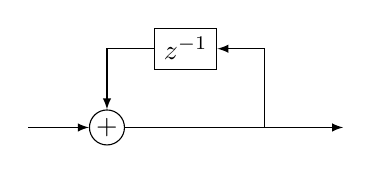
\begin{tikzpicture}
    \coordinate (in)  at (0,0);
    \coordinate (out) at (4,0);

    % branching coordinates
    \coordinate (b1) at (3,0);

    % Delay elements
    \node[draw] (d1) at  (2,1) {$z^{-1}$};

    % Adders
    \node[draw,circle, inner sep=0.3mm] (a1) at (1,0) {$+$};

    % Lines
    \draw[-latex] (in) -- (a1);
    \draw[-latex] (a1) -- (out);
    \draw[-latex] (b1) |- (d1);
    \draw[-latex] (d1) -| (a1);
\end{tikzpicture}

        \caption[Integrator Stage]{A single integrator stage}
        \label{fig:filtertopologies:integrator}
    \end{minipage}
    \begin{minipage}[t][][b]{0.45\textwidth}
        \centering
        \tikzsetnextfilename{combTopology}
% https://tex.stackexchange.com/a/183092/131649
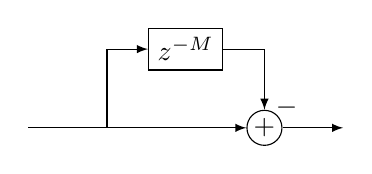
\begin{tikzpicture}
    \coordinate (in)  at (0,0);
    \coordinate (out) at (4,0);

    % branching coordinates
    \coordinate (b1) at (1,0);

    % Delay elements
    \node[draw] (d1) at (2,1) {$z^{-M}$};

    % Adder
    \node[draw,circle, inner sep=0.3mm] (a1) at (3,0) {$+$};

    % subtractors
    \node[above right=0.2ex] (s1) at (a1) {$-$};

    % Lines
    \draw[-latex] (in) -- (a1);
    \draw[-latex] (a1) -- (out);
    \draw[-latex] (b1) |- (d1);
    \draw[-latex] (d1) -| (a1);
\end{tikzpicture}

        \caption[Comb Stage]{A single comb stage in feedforward form}
        \label{fig:filtertopologies:comb}
    \end{minipage}
\end{figure}

\begin{figure}
    \centering
    %\tikzsetnextfilename{cicTopology}
% https://tex.stackexchange.com/a/183092/131649
\newcommand*\freqzFileCICB{images/cic/cic913.csv}
\newcommand*\freqzFileCombB{images/cic/comb913.csv}
\newcommand*\freqzFileIntB{images/cic/integrator3.csv}
\pgfplotstableread[col sep=comma]{\freqzFileIntB}\freqzTableIntB
\pgfplotstableread[col sep=comma]{\freqzFileCombB}\freqzTableCombB
\pgfplotstableread[col sep=comma]{\freqzFileCICB}\freqzTableCICB
\begin{tikzpicture}[
%    trim axis left,
%    trim axis right,
]
    \pgfplotsset{every axis/.style={
        height=20mm,
        grid=none,
        y filter/.code={\pgfmathparse{20*log10(\pgfmathresult))}},
        x filter/.code={\pgfmathparse{\pgfmathresult / 3.141592654}},
        %xlabel=Normalized Frequency,
        %ylabel=Magnitude,
        %x unit=\times\,\pi\,\si{\radian}/\si{\sample},
        %y unit=\si{dB},
        xtick={},
        xticklabels={},
        ytick={},
        yticklabels={},
        axis line style={draw=none},
        tick style={draw=none},
        },
    }

    \coordinate (in)  at  (0,0);
    \coordinate (out) at (10,0);

    % branching coordinates
    \coordinate (b1) at (2.25,0); % delta: 1.5
    \coordinate (b2) at (3.85,0); % delta: 1.5
    \coordinate (b3) at (5.8,0); % delta: 1.8
    \coordinate (b4) at (7.55,0); % delta: 1.5

    % Delay elements
    \node[draw] (d1) at  (1.6,1) {$z^{-1}$};
    \node[draw] (d2) at  (3.2,1) {$z^{-1}$};
    \node[draw] (d3) at  (6.5,1) {$z^{-M}$};
    \node[draw] (d4) at  (8.25,1) {$z^{-M}$};

    % Downsampler
    \node[draw] (r1) at (4.85,0) {$R\downarrow$};

    % Adders
    \node[draw,circle, inner sep=0.3mm] (a1) at  (1.1,0) {$+$};
    \node[draw,circle, inner sep=0.3mm] (a2) at  (2.7,0) {$+$};
    \node[draw,circle, inner sep=0.3mm] (a3) at  (7.05,0) {$+$};
    \node[draw,circle, inner sep=0.3mm] (a4) at  (8.8,0) {$+$};

    % subtractors
    \node[above right=0.2ex] (s1) at (a3) {$-$};
    \node[above right=0.2ex] (s2) at (a4) {$-$};

    % Lines
    \draw[-latex] (in) -- (a1);
    \draw[-latex] (a4) -- (out);
    \draw[-latex] (b1) |- (d1);
    \draw[-latex] (b2) |- (d2);
    \draw[-latex] (a1) -- (a2);
    \draw[-latex] (a2) -- (r1);
    \draw[-latex] (r1) -- (a3);
    \draw[-latex] (a3) -- (a4);
    \draw[-latex] (d1) -| (a1);
    \draw[-latex] (d2) -| (a2);
    \draw[-latex] (b3) |- (d3);
    \draw[-latex] (b4) |- (d4);
    \draw[-latex] (d3) -| (a3);
    \draw[-latex] (d4) -| (a4);

    % Annotations
    \node[above left =2.5ex] at (a1) {$f_s$};
    \node[above right=2.5ex] at (a4) {$f_s/R$};

    \begin{axis}[
            at = {(0,17mm)},
            xmin=0,
            xmax=1,
            ymin=-30,
            ymax=140,
            width=4.5cm,
            anchor=south west,
        ]
        \addplot[thick,q1,-] table[x=w, y=abs(H)] \freqzTableIntB;
    \end{axis}

    \begin{axis}[
            at = {(100mm,17mm)},
            xmin=0,
            xmax=1,
            ymin=-80,
            ymax=30,
            width=4.5cm,
            anchor=south east,
        ]
        \addplot[thick,q1,-] table[x=w, y=abs(H)] \freqzTableCombB;
    \end{axis}

    \begin{axis}[
            at = {(0,-4mm)},
            xmin=0,
            xmax=1,
            ymin=-80,
            ymax=65,
            width=10cm,
            anchor=north west,
        ]
        \addplot[thick,q1,-] table[x=w, y=abs(H)] \freqzTableCICB;
    \end{axis}
\end{tikzpicture}

    \caption[CIC Filter Topology]
        {CIC decimation filter topology with three integrator and comb stages}
    \label{fig:filtertopologies:cic}
\end{figure}

The integrator stages have a transfer function of
\begin{equation}
    \label{eq:cic:integrator_stage}
    H_I(z) = \frac{1}{1-z^{-1}}
\end{equation}

The comb stages run at the reduced frequency of $f_s/R$ and have the transfer
function
\begin{equation}
    \label{eq:cic:comb_stage}
    H_C(z) = 1 - z^{-RM}
\end{equation}
where  $M$  is the  \emph{differential  delay},  one  of the  filter's  design
parameters.

The  transfer function  of  a  complete CIC  filter  (referenced  to the  high
sampling rate  $f_s$) consisting of $N$  stages is deduced by  multiplying the
transfer functions of the $N$ cascaded integrator and comb stages, yielding
\begin{equation}
    \label{eq:cic:complete}
    H_{CIC}(z) = H_I^N(z) \cdot H_C^N(z) =
    \frac{\left(1 - z^{-RM}\right)^N}{\left( 1 - z^{-1} \right)^N} =
    \left[\sum_{k = 0}^{RM-1} z^{-k}\right]^N
\end{equation}

Looking at  the last form  of the CIC  filter's transfer function,  it becomes
evident  that it  is in  essence a  FIR filter  with unitary  coefficients. Of
particular note is the fact that this is so despite each stage having feedback
or feedforward paths and  the integrator stages having poles at  $f = 0$ (i.e.
the integrators  by themselves are  not in fact  BIBO stable, even  though the
complete  system  is). The  fact  that  the  resulting  filter  has  no  poles
can  be  intuitively   understood  by  looking  at   the  frequency  responses
of  the   integrator  and  comb   stages,  and  finally  their   cascade  (see
Section~\ref{subsubsec:cic:frequency_characteristics}).

CIC filters are well-suited to large reductions in sampling rates because they
are very  economical in  their resource  usage. This economy  is based  on six
primary factors (see also \cite{1163535}):
\begin{itemize}\tightlist
    \item
        The filter requires no multipliers.
    \item
        There are no filter coefficients to store.
    \item
        The amount  of storage needed  for intermediate results is  reduced by
        running the comb  stages at a lower sampling  rate. A conventional FIR
        filter topology implementing the  same transfer function would require
        more resources for storing its intermediate results because the entire
        filter would run at the incoming sampling rate.
    \item
        The  topology  of  the  filter   has  a  high  degree  of  regularity;
        consisting of two  primary building blocks. This lends  itself well to
        optimization.
    \item
        The control logic can be kept simple.
    \item
        The  same  filter  design can  be  used  for  a  large range  of  rate
        change  factors $R$,  requiring  minimal  adaption in  circuitry. This
        effect  can be  seen  in the  frequency response  plotted  in the  top
        plot of  Figure~\ref{fig:cic:freq_responses:var}.
\end{itemize}

However, CIC filters do suffer from some drawbacks. The two primary ones are:
\begin{itemize}\tightlist
    \item
        For    large     rate    change    factors    $R$,     the    register
        growth    of     the    filter    can    become     very    large. See
        Section~\ref{subsubsec:cic:register_growth}.
    \item
        A   CIC  filter   has   only  three   design  parameters   determining
        its   frequency  response: Rate   change   factor  $R$,   differential
        delay   $M$,    and   the    number   of   stages    $N$. The   amount
        of   fine-tuning   which   can    be   conducted   on   the   filter's
        frequency   response  is   therefore   extremely   limited  (more   in
        Section~\ref{subsubsec:cic:frequency_characteristics}).
\end{itemize}

As  can  be  seen in  Equation~\ref{eq:cic:integrator_stage},  the  integrator
stages have  unity feedback coefficients. In  the case of CIC  decimators, the
registers of  the integrators  will therefore  suffer from  register overflow.
This causes no harm as long as two conditions are fulfilled:
\begin{itemize}\tightlist
    \item
        The filter's  implementation is based  on two's complement  or another
        number system allowing wrap-around between  its most positive and most
        negative numbers.
    \item
        The maximum  magnitude which is expected  at the output is  within the
        range of that number system.
\end{itemize}

A numerical  example to demonstrate this  effect and better explain  the inner
workings  of a  CIC filter  can be  found in  Appendix~\ref{sec:app:cic_simu},
starting on page~\pageref{sec:app:cic_simu}.

% ==============================================================================
%
%              F R E Q U E N C Y   C H A R A C T E R I S T I C S
%
% ==============================================================================
\subsubsection{Frequency Characteristics} % ---------------------------------- %
\label{subsubsec:cic:frequency_characteristics}
% ---------------------------------------------------------------------------- %

This section presents some of  the more important frequency characteristics of
the  CIC  filter. We  will  start  with  some  considerations  about  how  the
integrators and comb  sections interact in the frequency domain  to create the
CIC filter's frequency response.

As  shown  in  the  topmost plot  in  Figure~\ref{fig:cic:freq_responses},  an
integrator is  in essence a lowpass  filter, with a pole  at $f = 0$.   A comb
filter is  a filter  which attenuates one  specific frequency  component along
with its multiples (in a notch comb  filter; there is also the inverse concept
of a  peak filter  which only  lets a  certain frequency  and multiples  of it
pass).  It is also  evident that comb filters have no poles  (a fact which can
be deduced from Equation~\ref{eq:cic:comb_stage} as well, of course).

Cascading integrators and  combs results in a frequency response  like the one
in the bottom  plot from Figure~\ref{fig:cic:freq_responses}. The integrator's
pole at $f = 0$ compensates for  the comb section's zero at the same location,
leading to a significant, but finite, DC gain of the CIC filter.

One drawback  of CIC  filters is  that they have  no clearly  defined passband
as  such. Rather,  their  frequency  response starts  dropping  off  right  as
the  frequency axis  goes  beyond  zero. This effect  (  also  referred to  as
\emph{passband  droop}  or  \emph{passband  attenuation}) is  visible  in  the
magnified section  of the  bottom plot  in Figure~\ref{fig:cic:freq_responses}
and  in   Figure~\ref{fig:cic:freq_responses:passband:attenuation}. Since  CIC
filters lack  a clearly defined  transition band edge, defining  the frequency
band which  is to  actually be  used, i.e.  the actual  passband, is  a design
decision  and can  vary even  when  using the  same filter,  depending on  the
application.

The  amount  of  passband  droop  is  constant for  a  given  product  of  the
differential  delay $M$  and  the cutoff  frequency $f_c$,  where  $f_c$ is  a
fraction  of the  lower sampling  rate (i.e.  a fraction  of the  first lobe's
width). Figure~\ref{fig:cic:freq_responses:passband:attenuation}    highlights
this  effect  for  two  different  filters. Table~\ref{tab:cic:pb_attenuation}
in                 Appendix~\ref{sec:app:cic_filter_tables}                 on
page~\pageref{tab:cic:pb_attenuation}  contains a  list with  more values  for
some common configurations.

Because  of the  passband droop,  a CIC  filer by  itself is  rarely a  viable
solution. Rather, it is generally deployed as  the first element in a chain of
filters,  where the  later stages  are FIR  filters. Due to  the CIC  filter's
frugality  in terms  of resource  usage, it  is ideally  suited as  an initial
stage, where the most samples per time need to be processed. The fact that FIR
filters need  to perform many  more computations  (and more complex  ones) per
sample is  then no longer as  much of a  problem, since those FIR  filters run
at  lower sampling  frequencies  and  have therefore  many  more clock  cycles
available  to  compute  each  output. Also,  because  the  frequency  response
of  a  FIR  filter can  be  very  finely  tuned  to a  desired  profile,  they
can  be used  to  compensate for  the  CIC filter's  passband  droop; this  is
generally  known as  a \emph{CIC  compensation filter}. More  on the  topic in
Section~\label{subsubsec:cic:compensators}.

Another  effect which  must be  taken  into consideration  when designing  CIC
filters  is  the amount  of  aliasing  which  occurs  from the  stopband  into
the  passband. A  region of  width  $f_c$  above  and  below each  $M$th  null
is  folded  back  into  the  filter's  passband. This  effect  is  highlighted
in  Figure~\ref{fig:cic:freq_responses:passband:aliasing}.    The  gravity  of
this  effect  depends   on  the  width  of  the  cutoff   frequency  $f_c$  as
well   as  the   differential  delay   $M$. Table~\ref{tab:cic:pb_attenuation}
Appendix~\ref{sec:app:cic_filter_tables}  contains  some   values  for  common
ranges for M and $f_c$.

As  mentioned, the  CIC filter  has  only three  design parameters: Its  rate
change factor  $R$, the differential delay  $M$ and the number  of stages $N$.
The influence  of these parameters  on the  CIC filter's frequency  response is
portrayed in Figure~\ref{fig:cic:freq_responses:var}. Some things of note are:
\begin{itemize}\tightlist
    \item
        Increasing $R$  increases the amount of  nulls as well as  the overall
        gain of the filter.
    \item
        Increasing  $M$ also  increases the  number of  nulls as  well as  the
        filter's gain.  Note that for  CIC decimators, the region around every
        $M$th null is folded back into the passband.

        For practical purposes, $M$ is usually  set to \num{1} or \num{2}, see
        \cite{1163535}.
    \item
        Adding more stages leads to a  high increase in filter gain, since $N$
        occurs in the exponent of the filter's transfer function. It does not,
        however, change the number or placement of the nulls.
\end{itemize}

\begin{figure}
    \centering
        %\tikzsetnextfilename{cicFreqResponsesStages}
\newcommand*\freqzFileIntB{images/cic/integrator3.csv}
\newcommand*\freqzFileCombB{images/cic/comb913.csv}
\newcommand*\freqzFileCICB{images/cic/cic913.csv}
\pgfplotstableread[col sep=comma]{\freqzFileIntB}\freqzTableIntB
\pgfplotstableread[col sep=comma]{\freqzFileCombB}\freqzTableCombB
\pgfplotstableread[col sep=comma]{\freqzFileCICB}\freqzTableCICB
\begin{tikzpicture}[
        %spy using outlines={magnification=4, connect spies}
        trim axis left,
        trim axis right,
    ]
     \pgfplotsset{every axis/.style={
            height=45mm,
            width=\textwidth,
            grid=none,
            y filter/.code={\pgfmathparse{20*log10(\pgfmathresult))}},
            x filter/.code={\pgfmathparse{\pgfmathresult / 3.141592654}},
            xlabel=Normalized Frequency,
            ylabel=Magnitude,
            x unit=\times\,\pi\,\si{\radian}/\si{\sample},
            y unit=\si{dB},
        },
        every axis legend/.append style={
            at={(1,-0.25)},  % if attached to bottom plot
            anchor=north east,
            cells={anchor=east},
        },
    }
    \begin{axis}[
            title=Integrator,
            at = {(0,0)},
            xmin=0,
            xmax=1,
            ymin=-30,
            ymax=140,
            xtick={0,0.5,1},
            ytick={120,100,80,60,40,20,0,-20},
            xticklabels={0,$f_s/4$,$f_s/2$},
        ]
        \addplot[thick,q1,-] table[x=w, y=abs(H)] \freqzTableIntB;
    \end{axis}

    \begin{axis}[
            title=Comb Filter,
            at = {(0,-65mm)},
            xmin=0,
            xmax=1,
            ymin=-80,
            ymax=30,
            xtick={0,0.5,1},
            ytick={20,0,-20,-40,-60},
            xticklabels={0,$f_s/4$,$f_s/2$},
        ]
        \addplot[thick,q1,-] table[x=w, y=abs(H)] \freqzTableCombB;
    \end{axis}

    \begin{axis}[
            title=CIC Filter,
            at = {(0,-130mm)},
            xmin=0,
            xmax=1,
            ymin=-80,
            ymax=65,
            xtick={0,0.5,1},
            ytick={60,40,20,0,-20,-40,-60},
            xticklabels={0,$f_s/4$,$f_s/2$},
        ]
        \addplot[thick,q1,-] table[x=w, y=abs(H)] \freqzTableCICB;

        %\coordinate (spypoint)     at (0.033,58);
        %\coordinate (magnifyglass) at (rel axis cs:0.123,-0.40);
    \end{axis}

    %\spy [black, width=3cm,height=1cm] 
    %    on (spypoint) in node[fill=white] at (magnifyglass);
    %\node[anchor=west,xshift=20mm] at (magnifyglass) {Passband Droop};
\end{tikzpicture}

        \caption[Frequency Responses for Integrators, Combs and CIC Filters]{%
            Frequency responses  for integrators, combs and  their combination
            into a three-stage CIC filter with a rate change factor of \num{9}
            and a  differential delay of  \num{1}.  Note that  \num{4.5} lobes
            fit into the plot for the comb  filter, due to $R\cdot M = 9$ (the
            order of the  comb filter).  The enlarged box shows  a close-up of
            the CIC filter's passband droop.%
        }
        \label{fig:cic:freq_responses}
\end{figure}

\begin{figure}
    \centering
        \tikzsetnextfilename{cicFreqResponsesVar}
\newcommand*\freqzFileCICA{images/cic/cic313.csv}
\newcommand*\freqzFileCICB{images/cic/cic913.csv}
\newcommand*\freqzFileCICC{images/cic/cic911.csv}
\newcommand*\freqzFileCICD{images/cic/cic921.csv}
\newcommand*\freqzFileCICE{images/cic/cic911.csv}
\newcommand*\freqzFileCICF{images/cic/cic913.csv}
\pgfplotstableread[col sep=comma]{\freqzFileCICA}\freqzTableCICA
\pgfplotstableread[col sep=comma]{\freqzFileCICB}\freqzTableCICB
\pgfplotstableread[col sep=comma]{\freqzFileCICC}\freqzTableCICC
\pgfplotstableread[col sep=comma]{\freqzFileCICD}\freqzTableCICD
\pgfplotstableread[col sep=comma]{\freqzFileCICE}\freqzTableCICE
\pgfplotstableread[col sep=comma]{\freqzFileCICF}\freqzTableCICF
\begin{tikzpicture}[
    trim axis left,
    trim axis right,
]
     \pgfplotsset{every axis/.style={
            height=45mm,
            width=\textwidth,
            grid=none,
            y filter/.code={\pgfmathparse{20*log10(\pgfmathresult))}},
            x filter/.code={\pgfmathparse{\pgfmathresult / 3.141592654}},
            xlabel=Normalized Frequency,
            ylabel=Magnitude,
            x unit=\times\,\pi\,\si{\radian}/\si{\sample},
            y unit=\si{\dB},
        },
        every axis legend/.append style={
            at={(0.02,0.05)},
            anchor=south west,
            cells={anchor=east},
        },
    }
    \begin{axis}[
            title=Influence of Rate Change $R$,
            at = {(0,0)},
            xmin=0,
            xmax=1,
            ymin=-100,
            ymax=65,,
            xtick={0,0.5,1},
            ytick={60,0,-60,-120},
            xticklabels={0,$f_s/4$,$f_s/2$},
        ]
        \addplot[thick,q1,-] table[x=w, y=abs(H)] \freqzTableCICA;
        \addplot[thick,q5,-] table[x=w, y=abs(H)] \freqzTableCICB;

        \legend{$R = 3$, $R = 9$};
    \end{axis}

    \begin{axis}[
            title=Influence of Differential Delay $M$,
            at = {(0,-65mm)},
            xmin=0,
            xmax=1,
            ymin=-40,
            ymax=30,
            xtick={0,0.5,1},
            ytick={20,0,-20,-40},
            xticklabels={0,$f_s/4$,$f_s/2$},
        ]
        \addplot[thick,q1,-] table[x=w, y=abs(H)] \freqzTableCICC;
        \addplot[thick,q5,-] table[x=w, y=abs(H)] \freqzTableCICD;

        \legend{$M = 1$, $M = 2$};
    \end{axis}

    \begin{axis}[
            title=Influence of Number of Stages $N$,
            at = {(0,-130mm)},
            xmin=0,
            xmax=1,
            ymin=-100,
            ymax=65,
            xtick={0,0.5,1},
            ytick={60,0,-60,-120},
            xticklabels={0,$f_s/4$,$f_s/2$},
        ]
        \addplot[thick,q1,-] table[x=w, y=abs(H)] \freqzTableCICE;
        \addplot[thick,q5,-] table[x=w, y=abs(H)] \freqzTableCICF;

        \legend{$N = 1$, $N = 3$};
    \end{axis}
\end{tikzpicture}

        \caption[Influence of Design Parameters on Frequency Response]{%
            The influence of  the design parameters $R$, $M$ and  $N$ on a CIC
            filter' frequency response.  Increasing $R$ and $M$, respectively,
            leads to an  increased number of nulls, as visible  in the top two
            plots,  as well  as  an  increase in  the  DC  gain.  Adding  more
            stages does  not change the  location of  the nulls, but  does add
            significant DC gain.%
        }
        \label{fig:cic:freq_responses:var}
\end{figure}

\begin{figure}
    \centering
        \newcommand*\freqzFileCICA{images/cic/pbattenuation914.csv}
\newcommand*\freqzFileCICB{images/cic/pbattenuation924.csv}
\pgfplotstableread[col sep=comma]{\freqzFileCICA}\freqzTableCICA
\pgfplotstableread[col sep=comma]{\freqzFileCICB}\freqzTableCICB
\begin{tikzpicture}[
        spy using outlines={magnification=4, connect spies}
    ]
     \pgfplotsset{every axis/.style={
            height=60mm,
            width=\textwidth,
            grid=none,
            y filter/.code={\pgfmathparse{20*log10(\pgfmathresult))}},
            x filter/.code={\pgfmathparse{\pgfmathresult / 3.141592654}},
            xlabel=Normalized Frequency,
            ylabel=Magnitude,
            x unit=\times\,\pi\,\si{\radian}/\si{\sample},
            y unit=\si{dB},
        },
    }
    \begin{axis}[
            title=Passband Droop in CIC Filters,
            at = {(0,0)},
            xmin=0,
            xmax=0.12,
            xtick={
                0.111111,
                0.055555,
                0.027777,
                0%
            },
            xticklabels={%
                $\frac{f_\mathrm{s,low}}{2}$,
                $\frac{f_\mathrm{s,low}}{4}$,
                $\frac{f_\mathrm{s,low}}{8}$,
                0%
            },
            ytick={
                0,
                -3.65,
                -10,
                -15
            },
            ymin=-15,
            ymax=1,
        ]
        \draw[da0,thick] (0      ,-3.65) -- (0.058   ,-3.65);
        \draw[da0,thick] (0.02777,-3)    -- (0.02777,-15);
        \draw[da0,thick] (0.05555,-3)    -- (0.05555,-15);

        \addplot[thick,q1,-] table[x=w, y=abs(H)] \freqzTableCICA;
        \addplot[thick,q3,-] table[x=w, y=abs(H)] \freqzTableCICB;
        \legend{%
            $M=1${,} $f_c = \frac{f_\mathrm{s,low}}{4}$,
            $M=2${,} $f_c = \frac{f_\mathrm{s,low}}{8}$
        };
    \end{axis}
\end{tikzpicture}

        \caption[CIC Filter: Passband and Aliasing Attenuation]{%
            Passband   attenuation   for   two   CIC   filters   with   $R=9$,
            $N=4$   and  $M=1$   and   $M=2$,  respectively. The   attenuation
            is  identical   for  the  bandwidth-differential   delay  product,
            which   is  $1/8$   for   both  of   these  configurations.    The
            attenuation   is  \SI{-3.65}{\dB}   in  both   cases;  the   value
            can    be   found    in   Table~\ref{tab:cic:pb_attenuation}    on
            page~\pageref{tab:cic:pb_attenuation}.%
        }
        \label{fig:cic:freq_responses:passband:attenuation}
\end{figure}

\begin{figure}
    \centering
        \newcommand*\freqzFileCICA{images/cic/pbAliasing914Complete.csv}
\newcommand*\freqzFileCICB{images/cic/pbAliasing914Null1Left.csv}
\newcommand*\freqzFileCICC{images/cic/pbAliasing914Null1Right.csv}
\newcommand*\freqzFileCICD{images/cic/pbAliasing914Null2Left.csv}
\newcommand*\freqzFileCICE{images/cic/pbAliasing914Null2Right.csv}
\newcommand*\freqzFileCICF{images/cic/pbAliasing914Null3Left.csv}
\newcommand*\freqzFileCICG{images/cic/pbAliasing914Null3Right.csv}
\newcommand*\freqzFileCICH{images/cic/pbAliasing914Null4Left.csv}
\newcommand*\freqzFileCICI{images/cic/pbAliasing914Null4Right.csv}
\pgfplotstableread[col sep=comma]{\freqzFileCICA}\freqzTableCICA
\pgfplotstableread[col sep=comma]{\freqzFileCICB}\freqzTableCICB
\pgfplotstableread[col sep=comma]{\freqzFileCICC}\freqzTableCICC
\pgfplotstableread[col sep=comma]{\freqzFileCICD}\freqzTableCICD
\pgfplotstableread[col sep=comma]{\freqzFileCICE}\freqzTableCICE
\pgfplotstableread[col sep=comma]{\freqzFileCICF}\freqzTableCICF
\pgfplotstableread[col sep=comma]{\freqzFileCICG}\freqzTableCICG
\pgfplotstableread[col sep=comma]{\freqzFileCICH}\freqzTableCICH
\pgfplotstableread[col sep=comma]{\freqzFileCICI}\freqzTableCICI
\begin{tikzpicture}[
        spy using outlines={magnification=3},
    ]
     \pgfplotsset{every axis/.style={
            height=140mm,
            width=\textwidth,
            grid=none,
        },
        every axis legend/.append style={
            at={(1,-0.15)},
            anchor=north east,
            cells={anchor=west},
        },
    }
    \begin{axis}[
            at = {(0,0)},
            y filter/.code={\pgfmathparse{20*log10(\pgfmathresult))}},
            x filter/.code={\pgfmathparse{\pgfmathresult / 3.141592654}},
            ylabel=$\left|H\right| (\si{\dB})$,
            xmin=0.001,
            xmax=1,
            ymin=-250,
            ymax=100,
            xtick={
                0,
                0.222222,
                0.444444,
                0.666666,
                0.888888,
                1%
            },
            xticklabels={%
                $0$,
                $1 \cdot f_\mathrm{s,low}$,
                $2 \cdot f_\mathrm{s,low}$,
                $3 \cdot f_\mathrm{s,low}$,
                $4 \cdot f_\mathrm{s,low}$,
                $f_\mathrm{s,high}/2$%
            },
        ]
        \fill[q0,opacity=0.20] ($(0.2222*0.75,100)$)        rectangle ($(0.2222*1.00,-250)$);
        \fill[q1,opacity=0.20] ($(0.2222*1.00,100)$)        rectangle ($(0.2222*1.25,-250)$);
        \fill[q2,opacity=0.20] ($(0.4444-0.2222*0.25,100)$) rectangle ($(0.4444+0.2222*0.00,-250)$);
        \fill[q3,opacity=0.20] ($(0.4444-0.2222*0.00,100)$) rectangle ($(0.4444+0.2222*0.25,-250)$);
        \fill[q4,opacity=0.20] ($(0.6666-0.2222*0.25,100)$) rectangle ($(0.6666+0.2222*0.00,-250)$);
        \fill[q5,opacity=0.20] ($(0.6666-0.2222*0.00,100)$) rectangle ($(0.6666+0.2222*0.25,-250)$);
        \fill[q6,opacity=0.20] ($(0.8888-0.2222*0.25,100)$) rectangle ($(0.8888+0.2222*0.00,-250)$);
        \fill[q7,opacity=0.20] ($(0.8888-0.2222*0.00,100)$) rectangle ($(0.8888+0.2222*0.25,-250)$);

        \fill[br0,opacity=0.50] (0,100) rectangle ($(0.2222*0.25,-250)$);
        \node[rotate=90,anchor=east] at ($(0.2222*0.25*0.5,-100)$) {%
            \footnotesize
            Passband: $f_c = 0.25 \cdot f_\mathrm{s,low}$
        };

        \draw[thick,da1] ($(0,76.31416-41.8)$) -- ($(0.2222*0.425,76.31416-41.8)$);
        \draw[thick,da1] (0,76.31416) -- ($(0.2222*0.425,76.31416)$);
        \draw[thick,da1,-latex] ($(0.2222*0.375,76.31416+5)$) -- ($(0.2222*0.375,76.31416)$);
        \draw[thick,da1] ($(0.2222*0.375,76.31416)$) -- ($(0.2222*0.375,76.31416-41.8)$);
        \draw[thick,da1,-latex] ($(0.2222*0.375,-50)$) -- ($(0.2222*0.375,76.31416-41.8)$);
        \node[thick,da1,rotate=90,anchor=north west] at ($(0.2222*0.375,-50)$) {\footnotesize\SI{41.8}{\dB}};

        \addplot[very thick,da1,-] table[x=w, y=abs(H)] \freqzTableCICA;
        \addplot[line cap=round,very thick,q0,-] table[x=w, y=abs(H)] \freqzTableCICB;
        \addplot[line cap=round,very thick,q1,-] table[x=w, y=abs(H)] \freqzTableCICC;
        \addplot[line cap=round,very thick,q2,-] table[x=w, y=abs(H)] \freqzTableCICD;
        \addplot[line cap=round,very thick,q3,-] table[x=w, y=abs(H)] \freqzTableCICE;
        \addplot[line cap=round,very thick,q4,-] table[x=w, y=abs(H)] \freqzTableCICF;
        \addplot[line cap=round,very thick,q5,-] table[x=w, y=abs(H)] \freqzTableCICG;
        \addplot[line cap=round,very thick,q6,-] table[x=w, y=abs(H)] \freqzTableCICH;
        \addplot[line cap=round,very thick,q7,-] table[x=w, y=abs(H)] \freqzTableCICI;

        \legend{%
            {},
            Left side of first null (flipped),
            Right side of first null (not flipped),
            Left side of second null (flipped),
            Right side of second null (not flipped),
            Left side of third null (flipped),
            Right side of third null (not flipped),
            Left side of fourth null (flipped),
            Right side of fourth null (not flipped),
        };

        %\coordinate (spypoint)     at (0.0300,9);
        %\coordinate (magnifyglass) at (rel axis cs:0.078,-0.35);
    \end{axis}

    %\spy [br0, width=1.9cm,height=5.3cm] 
    %    on (spypoint) in node[fill=white] at (magnifyglass);
\end{tikzpicture}

        \caption[CIC Filter: Passband and Aliasing Attenuation]{%
            Passband aliasing for  a CIC filter with $R =  9$, $N=4$ and $M=1$
            and a  cutoff frequency of $f_c  = 0.25$, referenced to  the lower
            sampling frequency $f_\mathrm{s,low}$.  The  region of width $f_c$
            around  every $M$th  null is  folded back  into the  passband. The
            regions beyond that  are of course folded back as  well, but since
            we choose to arbitrarily limit the passband, those regions are not
            of interest to us.  The resulting passband aliasing attenuation is
            \SI{41.8}{\dB}, as indicated in Table~\ref{tab:cic:pb_aliasing} on
            page~\pageref{tab:cic:pb_aliasing}.%
        }
        \label{fig:cic:freq_responses:passband:aliasing}
\end{figure}
% ==============================================================================
%
%                           C O M P E N S A T O R S
%
% ==============================================================================
\subsubsection{Compensators} % ----------------------------------------------- %
\label{subsubsec:cic:compensators}
% ---------------------------------------------------------------------------- %

In     order      to     achieve     a     flat      passband,     the     CIC
filter's    attenuation     in    the    frequency    range     observed    in
Figure~\ref{fig:cic:freq_responses:passband:attenuation}  can  be  compensated
with a filter  whose frequency response has the opposite  shape. Operated in a
cascade  (see Section~\ref{sec:multi_stage_filter_designs}),  the two  filters
create a frequency response with a flat passband and a sharp drop-off into the
stopband. Figure~\ref{fig:cic:cfir} shows  an example  of such a  system, with
frequency  responses of  a  CIC  filter, its  compensator,  and the  resulting
cascade.

The compensation filter not only serves to compensate for the passband, but is
also responsible  for the transition band  width of the cascade. Due  to their
flexibility, FIR filters are generally employed for this purpose. As mentioned
in  the previous  section,  the  sharpness of  their  transition  band can  be
controlled  by  adjusting  their  kernel size. If  the  compensator  has  more
filters  coming after  it in  the overall  filter chain,  its transition  band
need  not be  very narrow. A  filter  with a  few dozen  coefficients in  size
is  often  sufficient in  such  cases  (the filter  used  for  the example  in
Figure~\ref{fig:cic:cfir} has \num{50} coefficients).

The design of CIC compensators is  usually left up to software algorithms, for
example with Matlab. For a more detailed introduction to the topic, including
example  code  and  more  thorough  explanations,  Altera's  Application  Note
from~\cite{altera:an455} is warmly recommended.

\begin{figure}
    \centering
    \tikzsetnextfilename{cfirDemo}
\newcommand*\freqzFileCFIRA{images/cic/cfirDemoCascade.csv}
\newcommand*\freqzFileCFIRB{images/cic/cfirDemoCICAlone.csv}
\newcommand*\freqzFileCFIRC{images/cic/cfirDemoCFIRAlone.csv}
\newcommand*\freqzFileCFIRD{images/cic/cfirDemoCascadePBDetail.csv}
\newcommand*\freqzFileCFIRE{images/cic/cfirDemoCICAlonePBDetail.csv}
\newcommand*\freqzFileCFIRF{images/cic/cfirDemoCFIRAlonePBDetail.csv}
\pgfplotstableread[col sep=comma]{\freqzFileCFIRA}\freqzTableCFIRA
\pgfplotstableread[col sep=comma]{\freqzFileCFIRB}\freqzTableCFIRB
\pgfplotstableread[col sep=comma]{\freqzFileCFIRC}\freqzTableCFIRC
\pgfplotstableread[col sep=comma]{\freqzFileCFIRD}\freqzTableCFIRD
\pgfplotstableread[col sep=comma]{\freqzFileCFIRE}\freqzTableCFIRE
\pgfplotstableread[col sep=comma]{\freqzFileCFIRF}\freqzTableCFIRF
\begin{tikzpicture}[
    trim axis left,
    trim axis right,
]
     \pgfplotsset{every axis/.style={
            height=45mm,
            width=\textwidth,
            grid=none,
            y filter/.code={\pgfmathparse{20*log10(\pgfmathresult))}},
            x filter/.code={\pgfmathparse{\pgfmathresult / 3.141592654}},
            xlabel=Normalized Frequency,
            ylabel=Magnitude,
            x unit=\times\,\pi\,\si{\radian}/\si{\sample},
            y unit=\si{\dB},
            legend columns=3,
            unbounded coords = jump,
        },
    }
    \begin{axis}[
            at = {(0,0)},
            title = {CIC Compensation Overview},
            xmin=0,
            xmax=1,
            ymin=-100,
            ymax=115,
            xtick={0,0.06667,0.25,0.5,0.75,1},
        ]
        \addplot[thick,q5,-] table[x=w, y=abs(H)] \freqzTableCFIRB;
        \addplot[thick,ct4,-] table[x=w, y=abs(H)] \freqzTableCFIRC;
        \addplot[thick,q1,-] table[x=w, y=abs(H)] \freqzTableCFIRA;
        \legend{CIC Filter, Compensator, Cascade};
    \end{axis}
    \begin{axis}[
            at = {(0,-65mm)},
            title = {Passband Detail (Gain Normalized)},
            legend pos=south west,
            xmin=0,
            xmax=0.078,
            ymax=10,
            ymin=-20,
            xtick={0,0.025,0.05,0.075},
        ]
        \addplot[thick,q5,-] table[x=w, y=abs(H)] \freqzTableCFIRE;
        \addplot[thick,ct4,-] table[x=w, y=abs(H)] \freqzTableCFIRC;
        \addplot[thick,q1,-] table[x=w, y=abs(H)] \freqzTableCFIRD;
        \legend{CIC Filter, Compensator, Cascade};
    \end{axis}
\end{tikzpicture}

    \caption[CIC Compensator]{%
        Frequency behavior of  a CIC filter, its compensator,  and the cascade
        of the  two. Note the  spectral copies of  the compensator  around the
        nulls of the  CIC filter, i.e. the multiples of  its outgoing sampling
        rate.%
    }
    \label{fig:cic:cfir}
\end{figure}
% ==============================================================================
%
%                        R E G I S T E R   G R O W T H
%
% ==============================================================================
\subsubsection{Register Growth}
\label{subsubsec:cic:register_growth}

As shown by Hogenauer in~\cite{1163535}, the maximum register growth is
\begin{equation}
    \label{eq:cic:maximum_register_growth}
    G_\mathrm{max} = (R \cdot M)^N
\end{equation}
The most  significant bit $B_\mathrm{max}$ of  the output register as  well as
for all  stages (both the  integrators and the comb  stages) of the  filter is
determined to be
\begin{equation}
    \label{eq:cic:maximum_register_growth:bit_width}
    B_\mathrm{max} = \lceil N \log_2 RM + B_\mathrm{in} - 1 \rceil
\end{equation}
where $B_\mathrm{in}$ is  the bit width of the input  register.  For high rate
change  factors, these  values can  become very  large.  A  filter with  three
stages, a  differential delay of  \num{1}, a rate  change of \num{128}  and an
input  width of  \num{16}\,bits  yields  \num{36}\,bits output  width at  full
precision.
% ==============================================================================
%
%         T R U N C A T I O N   A N D   R O U N D I N G   E R R O R S
%
% ==============================================================================
\subsubsection{Errors Due to Truncation and Rounding}
\label{subsubsec:cic:truncation_and_rounding}

In practical cases, it is often not feasible to retain full precision; in such
situations, either truncation or rounding may  be used at each filter stage to
reduce register widths and keep resource usage within certain limits. For this
purpose, it is necessary  to know the system function from  the $j$th stage up
to and including the last:
\begin{equation}
    \label{eq:cic:truncation_rounding:system_function}
    H_j(z) = \left\lbrace
        \begin{aligned}
            H_I^{N-j+1}H_C^N                        &
            = \sum_{k=0}^{(RM-1)N+j-1} h_j[k]z^{-k} &
            \quad j                                 &
            = 1, 2, \cdots, N                       \\
            H_C^{j-N}                                          &
            = \hspace{1.1em}\sum_{k=0}^{2N+1-j} h_j[k]z^{-kRM} &
            \quad j                                            &
            = N+1, \cdots, 2N
        \end{aligned}
    \right.
\end{equation}
where
\begin{equation}
    \label{eq:cic:truncation_rounding:system_function}
    h_j[k] = \left\lbrace
        \begin{aligned}
            \sum_{l=0}^{\lfloor k/(RM) \rfloor} (-1)^l
            {{N}\choose{l}}{{N-j+k-RMl}\choose{k = RMl}} &
            j                                            &
            = 1, 2, \cdots N                             \\
            (-1)^k{{2N+1-j}\choose{k}} &
            j                          &
            = N+1, \cdots 2N
        \end{aligned}
    \right.
\end{equation}
are the  impulse response  coefficients. These functions  are also  derived by
Hogenauer in~\cite{1163535}.

In a  filter with $N$ stages,  there are $2N+1$  error sources in the  case of
limited precision: Each stage,  and the output register. Each  error source is
presumed to have  white noise characteristics, i.e. its  noise is uncorrelated
to its input as well as other error sources.  The error at the $j$th source is
assumed to have a uniform probability distribution with a width of
\begin{equation}
    \label{eq:cic:truncation_rounding:probability_distribution}
    E_j = \left\lbrace
        \begin{aligned}
            0        & \quad\text{without truncation or rounding}\\
            2^{B_j}  & \quad\text{otherwise}
        \end{aligned}
    \right.
\end{equation}
where the number of bits discarded at the $j$th error source is $B_j$. The mean
of this error is
\begin{equation}
    \label{eq:cic:truncation_rounding:mean}
    \mu_j = \left\lbrace
        \begin{aligned}
            \frac{1}{2}E_j & \quad\text{for truncation}\\
            0              & \quad\text{otherwise}
        \end{aligned}
    \right.
\end{equation}
and the variance comes out to
\begin{equation}
    \label{eq:cic:truncation_rounding:variance}
    \sigma_j^2 = \frac{1}{12}E_j^2.
\end{equation}

The total mean error at the filter's output due to the $j$th stage is
\begin{equation}
    \label{eq:cic:truncation_rounding:total_mean_error_jth_stage}
    \mu_{T_j} = \mu_jD_j
\end{equation}
where
\begin{equation}
    \label{eq:cic:truncation_rounding:mean_error_gain}
    D_j = \left\lbrace
        \begin{aligned}
            (RM)^N         & \quad j = 1\\
            0              & \quad j = 2, 3, \cdots, 2N\\
            1              & \quad j = 2N+1
        \end{aligned}
    \right.
\end{equation}
is the \emph{mean  error gain} for the $j$th error  source. Note that only the
first and the last  error source contribute to the filter's  mean error at the
output. This is because  the sum of the impulse response  coefficients is zero
for all other  stages. Consequently, whether one chooses to  truncate or round
is  without  consequence except  in  the  case of  the  first  and last  error
sources. In an analogous manner, the total variance computes to
\begin{equation}
    \label{eq:cic:truncation_rounding:total_variance_jth_stage}
    \sigma_{T_j}^2 = \sigma_j^2F_j^2
\end{equation}
where
\begin{equation}
    \label{eq:cic:truncation_rounding:variance_error_gain}
    F_j = \left\lbrace
        \begin{aligned}
            \sum_k h_j^2[k]  & \quad j = 1, 2, \cdots, 2N\\
            1                & \quad j = 2N+1
        \end{aligned}
    \right.
\end{equation}
is called the \emph{variance error gain} for the $jth$ error source.

We can now compute the global mean error and variance of the filter:
\begin{align}
    \label{eq:cic:truncation_rounding:global:mean_error}
    \mu_T &= \sum_{j = 1}^{2N+1} \mu_{T_j} = \mu_{T_1} + \mu_{T_{2N+1}}\\
    \label{eq:cic:truncation_rounding:global:variance}
    \sigma_{T}^2 &= \sum_{j=1}^{2N+1} \sigma_{T_j}
\end{align}
These equations  are used  to calculate  the properties of  the CIC  filter as
deployed in our design, see Section~\ref{subsec:fpga:errors_in_cic_filter}.

% ==============================================================================
%
%                   C I C   F I L T E R S :   S U M M A R Y
%
% ==============================================================================
\subsubsection{Summary}
\label{subsubsec:cic:summary}

In conclusion, the key properties of CIC filters are:
\begin{itemize}\tightlist
    \item
        They can be implemented both as decimators and interpolators.
    \item
        Neither multipliers nor storage for coefficients are needed.
    \item
        CIC  decimation  filters have  a  high  gain, leading  to  significant
        register  growth.  Truncation  or rounding  can be  used to  limit the
        resource usage, both at the filter's output and internally.
    \item
        The three design parameters are  the rate change $R$, the differential
        delay $M$ and the number of stages $N$.
    \item
        The  presence of  passband  droop requires  a  compensation filter  to
        achieve a flat passband response.
\end{itemize}
%>>>

%>>>

% ==============================================================================
%
%             M U L T I - S T A G E   F I L T E R   D E S I G N S
%
% ==============================================================================
\section{Multi-Stage Filter Designs} % <<< ----------------------------------- %
\label{sec:multi_stage_filter_designs}
% ---------------------------------------------------------------------------- %

At  first   sight,  the   most  obvious  way   to  implement   a  downsampling
system  might  appear  to be  to  design  one  filter  for each  desired  rate
change   factor.   However,   this  would   be  highly   impractical. Instead,
multi-stage  designs  are usually  used  in  practice. An in-depth  discussion
of  their  advantages and  drawbacks  was  offered  by Crochiere  and  Rabiner
in~\cite{crochiere-rabiner:multirate-dsp}. A few aspects of multi-stage filter
design which are relevant to our application shall be presented here.

To  reduce  aliasing  effects  in  the passband,  it  is  generally  desirable
to  keep  the width  of  the  transition  band  roughly constant  in  relation
to  the   width  of   the  passband   (visible  in   the  filter's   flank  in
Figure~\ref{fig:aliasing:iirCopies}).   As  the downsampling  ratio  increases
and  the  passband width  decreases,  the  transition band  therefore  becomes
progressively narrower,  necessitating higher filter orders  in a single-stage
design.

This   effect  is   illustrated  in   Figure~\ref{fig:fdesign:tbw_width_Rvar},
comparing two filters with a transition band $1/5$ as wide as the passband for
downsampling  ratios of  \num{2} and  \num{4}. The filter  for $R=4$  requires
\num{60}  coefficients,  compared  to  \num{30} coefficients  for  the  filter
designed  for $R=2$.   The other  specifications (passband  ripple, stop  band
attenuation) are identical.   As an extreme case, a filter  designed by Matlab
with the  same parameters for  a downsampling  ratio of $R=625$  is \num{8860}
coefficients in size.

Using multi-stage  designs helps to avoid  the need to implement  filters with
such large kernels.  When cascading filters, it is the last stage of the chain
which defines the overall passband and transition band width. The same overall
transition band  in absolute  terms can  be achieved  with smaller  filters in
multi-stage designs, because  a filter's transition band width  is relative to
the sampling rate at which it is running.  This is shown in the bottom plot in
Figure~\ref{fig:fdesign:tbw_width_Rvar}.

\begin{figure}
    \centering
    \newcommand*\freqzFileTBWA{images/fdesign/tbw-fs-wide.csv}
\newcommand*\freqzFileTBWB{images/fdesign/tbw-fs-narrow.csv}
\newcommand*\freqzFileTBWC{images/fdesign/cascade-of-wide.csv}
\pgfplotstableread[col sep=comma]{\freqzFileTBWA}\freqzTableTBWA
\pgfplotstableread[col sep=comma]{\freqzFileTBWB}\freqzTableTBWB
\pgfplotstableread[col sep=comma]{\freqzFileTBWC}\freqzTableTBWC
\begin{tikzpicture}
     \pgfplotsset{every axis/.style={
            height=60mm,
            width=\textwidth,
            grid=none,
            ylabel=Magnitude,
            xlabel=Normalized Frequency,
            xmin=0,
            xmax=1,
            ymax=5,
            ymin=-100,
            y filter/.code={\pgfmathparse{20*log10(\pgfmathresult))}},
            x filter/.code={\pgfmathparse{\pgfmathresult / 3.141592654}},
            x unit=\times\,\pi\,\si{\radian}/\si{\sample},
            y unit=\si{dB},
            xticklabel style={font=\footnotesize},
            ytick={0,-40,-80},
        },
    }
    \begin{axis}[
            title={Filter for Rate Change $R=2$, Coefficient Count $N=30$},
            at = {(0,0)},
            xtick={0,0.5,0.6,1},
            xticklabels={0,0.5,0.6,$f_\mathrm{s1}/2$},
        ]
        \fill[dv-2] (0.5,5) rectangle (0.6,-100);
        \addplot[thick,q1,-] table[x=W, y=abs(H)] \freqzTableTBWA;
    \end{axis}
    \begin{axis}[
            title={Filter for Rate Change $R=4$, Coefficient Count $N=60$},
            at = {(0,-70mm)},
            xtick={0,0.25,0.3,1},
            xticklabels={0,0.25,0.30,$f_\mathrm{s1}/2$},
        ]
        \fill[dv-2] (0.25,5) rectangle (0.3,-100);
        \addplot[thick,q1,-] table[x=W, y=abs(H)] \freqzTableTBWB;
    \end{axis}
    \begin{axis}[
            title={Cascade of Filters with $N=30$ Per Filter for Rate Change $R=4$},
            at = {(0,-140mm)},
            xtick={
                0,
                0.25,
                0.3,
                0.5,
                0.6,
                1
            },
            xticklabels={
                0,
                0.25,
                0.30,
                $f_\mathrm{s2}/2$,
                0.60,
                $f_\mathrm{s1}/2$
            },
        ]
        \fill[dv-2] (0.25,5) rectangle (0.3,-100);
        \fill[gray!20!white] (0.50,5) rectangle (0.6,-100);
        \addplot[thin,gray,dashed,-] table[x=W, y=abs(H)] \freqzTableTBWA;
        \addplot[thick,q1,-] table[x=W, y=abs(H)] \freqzTableTBWC;
        \legend{Stage 1,Cascade};
    \end{axis}
\end{tikzpicture}

    \caption
        [Frequency Response of Multi-Stage Vs. Single-Stage Design]{%
        Two filters are  used here: Both have a transition band  $1/5$ as wide
        as  their passbands. The  top filter  is designed  for a  downsampling
        ratio $R=2$ and  has a coefficient count of  $N=30$. The second filter
        is designed for $R=4$ and  has \num{60} coefficients. Cascading two of
        the top filters into a two-stage  design, depicted in the bottom plot,
        results in the same overall passband  and transition band width as the
        single-stage design.%
    }
    \label{fig:fdesign:tbw_width_Rvar}
\end{figure}

Since  cascading  multiple  filters   does  increase  coefficient  count  (and
storage), one might  be inclined to think that not  much has been won. Indeed,
the  overall  number  of  coefficients   is  identical  for  both  filters  in
Figure~\ref{fig:fdesign:tbw_width_Rvar}  (though, this  obviously need  not be
so  in  other  examples). However: Merely \num{30}  multipliers  and  \num{29}
adders  (those  of the  first  filter  in the  cascade)  run  at the  incoming
sampling  frequency in  the  case  of the  cascade,  while  the components  of
the  second  filter  run at  half  that.   In  the  case of  the  single-stage
filter,  all  its  \num{60}  multipliers   and  \num{59}  adders  run  at  the
full  sampling frequency. Distributing  the calculations  over two  stages has
therefore yielded  an overall reduction  in needed computation  power. As rate
change  factors increase,  the  benefits of  multi-stage  designs become  even
more pronounced~\cite{crochiere-rabiner:multirate-dsp}. 

In general, the  earlier stages in a cascade tend  to have higher downsampling
ratios  but  wider   transition  bands,  and  the  later   stages  have  lower
downsampling  ratios  and  narrower  transition  bands  (normalized  to  their
respective  sampling frequencies).   This  minimizes  computations across  the
overall design by  using smaller filters for  high-frequency calculations, and
giving the larger filters more  time to compute their outputs. Multiple stages
having the  same downsampling  ratios is  also a  valid approach,  but earlier
stages having lower downsampling ratios than later stages is uncommon.

Another advantage of  cascading filters is that successive stages  can be used
to  shape the  overall frequency  response, as  seen in  the case  of the  CIC
compensator in Section~\ref{subsubsec:cic:compensators} A drawback of cascades
is that the ripple in their passband shows additive behavior, so the stages in
a cascade of  filters have more stringent ripple requirements  in the passband
then  a single-stage. However,  the cost  for this  is usually  offset by  the
advantages of multi-stage designs.

When designing multi-stage filters, it can  happen that the transition band of
an earlier stage overlaps with the spectral copy of a later stage running at a
reduced sampling rate.  In that case, the stopband response of the cascade can
have  peaks exceeding  the  desired overall  stopband attenuation. To  prevent
this, the following condition must be satisfied:
\begin{equation}
    \label{eq:cascade:transition_band_overlap}
    f_\mathrm{st,1} < \frac{f_\mathrm{s,1} - f_\mathrm{st,2}}{R_1}
\end{equation}
\begin{conditions}
    f_\mathrm{s,1}  & high sampling rate                  \\
    f_\mathrm{st,1} & stopband frequency of first filter  \\
    f_\mathrm{st,2} & stopband frequency of second filter \\
    R_1             & rate reduction in first filter      \\
\end{conditions}
Figure~\ref{fig:fdesign:cascade:good_vs_bad}  shows  some  examples  for  this
condition being broken or fulfilled.

\begin{figure}
    \centering
    \tikzsetnextfilename{cascadeTBOverlap}
\newcommand*\freqzFileCascA{images/fdesign/cascadeDemoHBGoodCascade.csv}
\newcommand*\freqzFileCascB{images/fdesign/cascadeDemoHBGoodStage1.csv}
\newcommand*\freqzFileCascC{images/fdesign/cascadeDemoHBGoodStage2.csv}
\newcommand*\freqzFileCascD{images/fdesign/cascadeDemoHBBadCascade.csv}
\newcommand*\freqzFileCascE{images/fdesign/cascadeDemoHBBadStage1.csv}
\newcommand*\freqzFileCascF{images/fdesign/cascadeDemoHBBadStage2.csv}
\pgfplotstableread[col sep=comma]{\freqzFileCascA}\freqzTableCascA
\pgfplotstableread[col sep=comma]{\freqzFileCascB}\freqzTableCascB
\pgfplotstableread[col sep=comma]{\freqzFileCascC}\freqzTableCascC
\pgfplotstableread[col sep=comma]{\freqzFileCascD}\freqzTableCascD
\pgfplotstableread[col sep=comma]{\freqzFileCascE}\freqzTableCascE
\pgfplotstableread[col sep=comma]{\freqzFileCascF}\freqzTableCascF
\begin{tikzpicture}[
    trim left=(plot1.north west).
    trim right=(plot6.south east).
]
     \pgfplotsset{every axis/.style={
            height=30mm,
            width=\textwidth,
            grid=none,
            y filter/.code={\pgfmathparse{20*log10(\pgfmathresult))}},
            x filter/.code={\pgfmathparse{\pgfmathresult / 3.141592654}},
            xlabel=Normalized Frequency,
            ylabel=Magnitude,
            x unit=\times\,\pi\,\si{\radian}/\si{\sample},
            y unit=\si{dB},
            ymax=5,
            ymin=-100,
            xmin=0,
            xmax=1,
            xmajorgrids=true,
            ymajorgrids=true,
            ytick={
                0,
                -40,
                -80
            },
        },
    }
    \begin{axis}[
            title={Cascade Without Peak in Stopband},
            name=plot1,
            at = {(0,0)},
            xtick={
                0,
                0.175,
                0.325,
                0.5,
                1
            },
            xticklabels={
                0,
                0.175,
                0.325,
                $f_{s2}/2$,
                $f_{s1}/2$
            },
        ]
        \addplot[thick,q1,-] table[x=W, y=abs(H)] \freqzTableCascA;
        \addplot[thin,gray,dashed,-] table[x=W, y=abs(H)] \freqzTableCascB;
        \addplot[thin,gray,dashed,-] table[x=W, y=abs(H)] \freqzTableCascC;
    \end{axis}
    \begin{axis}[
            title={Cascade With Peak in Stopband},
            at = {(0,-50mm)},
            xtick={
                0,
                0.1,
                0.4,
                0.5,
                1
            },
            xticklabels={
                0,
                0.2,
                0.4,
                $f_{s2}/2$,
                $f_{s1}/2$
            },
        ]
        \addplot[thick,q5,-] table[x=W, y=abs(H)] \freqzTableCascD;
        \addplot[thin,gray,dashed,-] table[x=W, y=abs(H)] \freqzTableCascE;
        \addplot[thin,gray,dashed,-] table[x=W, y=abs(H)] \freqzTableCascF;
    \end{axis}
    \begin{axis}[
            title=Stage 1 (No Peak),
            width=0.47\textwidth,
            at = {(0,-100mm)},
            xtick={
                0,
                0.35,
                0.50,
                0.65,
                1
            },
            xticklabels={
                0,
                0.35,
                0.50,
                0.65,
                $f_{s1}/2$
            },
        ]
        \addplot[thick,q1,-] table[x=W, y=abs(H)] \freqzTableCascB;
    \end{axis}
    \begin{axis}[
            title=Stage 1 (Peak),
            width=0.47\textwidth,
            at = {(0.53\textwidth,-100mm)},
            xtick={
                0,
                0.2,
                0.5,
                0.8,
                1
            },
            xticklabels={
                0,
                0.2,
                $f_{s2}/2$,
                0.8,
                $f_{s1}/2$
            },
            ylabel={},
            y unit={},
            yticklabel pos=right,
            yticklabel style={font=\footnotesize},
        ]
        \addplot[thick,q5,-] table[x=W, y=abs(H)] \freqzTableCascE;
    \end{axis}
    \begin{axis}[
            title=Stage 2 (No Peak),
            width=0.47\textwidth,
            at = {(0,-150mm)},
            xtick={
                0,
                0.175,
                0.325,
                0.5,
                0.675,
                0.825,
                1
            },
            xticklabels={
                0,
                0.175,
                0.325,
                0.500,
                0.675,
                0.825,
                $f_{s1}/2$
            },
        ]
        \addplot[thick,q1,-] table[x=W, y=abs(H)] \freqzTableCascC;
    \end{axis}
    \begin{axis}[
            title=Stage 2 (Peak),
            name=plot6,
            width=0.47\textwidth,
            at = {(0.53\textwidth,-150mm)},
            xtick={
                0,
                0.1,
                0.4,
                0.5,
                0.6,
                0.9,
                1
            },
            xticklabels={
                0,
                0.1,
                0.4,
                $f_{s2}/2$,
                0.6,
                0.9,
                $f_{s1}/2$
            },
            ylabel={},
            y unit={},
            yticklabel pos=right,
            yticklabel style={font=\footnotesize},
        ]
        \addplot[thick,q5,-] table[x=W, y=abs(H)] \freqzTableCascF;
    \end{axis}
\end{tikzpicture}

    \caption[Cascade: Transition Band Overlap]{%
        Comparison   of   two   cascades: The   first   cascade   (blue)   has
        sufficient  distance   between  the  start  of   its  stopband  ($0.65
        \cdot  f_\mathrm{s1}$)  and  the  start  of  the  transition  band  of
        the  second stage's  first copy  around $f_\mathrm{s2}$  ($0.675 \cdot
        f_\mathrm{s1}$). The  second  cascade  (orange)  has  a  peak  in  its
        stopband because the transition band  of its first stage overlaps with
        the  copy of  the second  stage ($0.8  \cdot f_\mathrm{s1}$  vs.  $0.6
        \cdot f_\mathrm{s1}$). \emph{Note:} All  frequencies are referenced to
        the high sampling rate $f_\mathrm{s1}$.%
    }
    \label{fig:fdesign:cascade:good_vs_bad}
\end{figure}

One last effect of note when cascading filters concerns stopband attenuation:
When cascading two filters with different stopband attenuations, two things
can happen:
\begin{itemize}\tightlist
    \item
        The second  filter attenuates more  strongly than the  first one. This
        results  in  peaks  above  the second  filter's  stopband  attenuation
        in  the regions  where  the  spectral copies  of  the second  filter's
        passband  are   located. This  can  be   seen  in  the  top   plot  in
        Figure~\ref{fig:fdesign:cascade:ast_demo}.
    \item
        The first filter attenuates more  strongly than the first one. In that
        case, the stopband region of the  cascade right next to its transition
        band is  less strongly  attenuated than  the stopband  regions farther
        away  from  the  edge. This  case  is shown  in  the  middle  plot  in
        Figure~\ref{fig:fdesign:cascade:ast_demo}.
\end{itemize}
Either  of  these  two  effects   is  usually  not  desired,  barring  special
scenarios. In both  cases, the  resources invested  into the  steeper filter's
stronger  attenuation  are  wasted  by  the  other  filter's  weaker  stopband
attenuation. It therefore makes more sense for the various stages in a cascade
to have the same stopband attenuation, in general.

\begin{figure}
    \centering
    \tikzsetnextfilename{cascadeAstMismatch}
\newcommand*\freqzFileAstA{images/fdesign/ast-60.csv}
\newcommand*\freqzFileAstB{images/fdesign/ast-40.csv}
\newcommand*\freqzFileAstC{images/fdesign/ast-40-60.csv}
\newcommand*\freqzFileAstD{images/fdesign/ast-60-40.csv}
\newcommand*\freqzFileAstE{images/fdesign/ast-60-ref-high.csv}
\newcommand*\freqzFileAstF{images/fdesign/ast-40-ref-high.csv}
\pgfplotstableread[col sep=comma]{\freqzFileAstA}\freqzTableAstA
\pgfplotstableread[col sep=comma]{\freqzFileAstB}\freqzTableAstB
\pgfplotstableread[col sep=comma]{\freqzFileAstC}\freqzTableAstC
\pgfplotstableread[col sep=comma]{\freqzFileAstD}\freqzTableAstD
\pgfplotstableread[col sep=comma]{\freqzFileAstE}\freqzTableAstE
\pgfplotstableread[col sep=comma]{\freqzFileAstF}\freqzTableAstF
\begin{tikzpicture}[
    trim left=(plot1.north west).
    trim right=(plot4.south east).
]
     \pgfplotsset{every axis/.style={
            height=45mm,
            width=\textwidth,
            grid=none,
            ylabel=Magnitude,
            xlabel=Normalized Frequency,
            xmin=0,
            xmax=1,
            ymax=5,
            ymin=-100,
            y filter/.code={\pgfmathparse{20*log10(\pgfmathresult))}},
            x filter/.code={\pgfmathparse{\pgfmathresult / 3.141592654}},
            x unit=\times\,\pi\,\si{\radian}/\si{\sample},
            y unit=\si{dB},
            xticklabel style={font=\footnotesize},
            ytick={0,-40,-80},
        },
    }
    % 40 -> 60
    \begin{axis}[
            name=plot1,
            title={Stage 1: \SI[detect-all,mode=text]{40}{\dB}, Stage 2: \SI[detect-all,mode=text]{60}{\dB}},
            at = {(0,0)},
            ytick={0,-40,-60},
            %xtick={0,0.5,0.6,1},
            %xticklabels={0,0.5,0.6,$f_\mathrm{s1}/2$},
        ]
        \addplot[thin,gray,dashed,-] table[x=W, y=abs(H)] \freqzTableAstE;
        \addplot[thin,gray,dashed,-] table[x=W, y=abs(H)] \freqzTableAstB;
        \addplot[thick,q1,-] table[x=W, y=abs(H)] \freqzTableAstC;
    \end{axis}
     60 -> 40
    \begin{axis}[
            title={Stage 1: \SI[detect-all,mode=text]{60}{\dB}, Stage 2: \SI[detect-all,mode=text]{40}{\dB}},
            at = {(0,-65mm)},
            ytick={0,-40,-60},
            %xtick={0,0.5,0.6,1},
            %xticklabels={0,0.5,0.6,$f_\mathrm{s1}/2$},
        ]
        \addplot[thin,gray,dashed,-] table[x=W, y=abs(H)] \freqzTableAstF;
        \addplot[thin,gray,dashed,-] table[x=W, y=abs(H)] \freqzTableAstA;
        \addplot[thick,q1,-] table[x=W, y=abs(H)] \freqzTableAstD;
    \end{axis}
    % 60 dB
    \begin{axis}[
            title={\SI[detect-all,mode=text]{60}{\dB} Stopband Attenuation},
            width=0.47\textwidth,
            at = {(0,-130mm)},
            ytick={0,-60},
            %xtick={0,0.5,0.6,1},
            %xticklabels={0,0.5,0.6,$f_\mathrm{s1}/2$},
        ]
        \addplot[thick,q1,-] table[x=W, y=abs(H)] \freqzTableAstA;
    \end{axis}
    % 40 dB
    \begin{axis}[
            title={\SI[detect-all,mode=text]{40}{\dB} Stopband Attenuation},
            name=plot4,
            width=0.47\textwidth,
            at = {(0.53\textwidth,-130mm)},
            ylabel={},
            y unit={},
            yticklabel pos=right,
            yticklabel style={font=\footnotesize},
            %xtick={0,0.5,0.6,1},
            %xticklabels={0,0.5,0.6,$f_\mathrm{s1}/2$},
        ]
        \addplot[thick,q1,-] table[x=W, y=abs(H)] \freqzTableAstB;
    \end{axis}
\end{tikzpicture}

    \caption[Cascade: Stopband Attenuation]{%
        Cascading  two  filters  with different  stopband  attenuations: If  a
        filter with stronger  stopband attenuation is cascaded  after a filter
        with weaker  attenuation, the  resultant cascade  has peaks  above the
        second  filter's  stopband  attenuation (top  plot). If  the  stronger
        filter is  first in the  cascade, the  drop-off in the  stopband right
        next to the  transition band is weaker. The two  filters by themselves
        are shown in the bottom plots.%
    }
    \label{fig:fdesign:cascade:ast_demo}
\end{figure}

%>>>

%^^A vim: foldenable foldcolumn=4 foldmethod=marker foldmarker=<<<,>>>

% ------------------------------------------------------------------------->>> %
% <<< ---------------------------------------------------------------- MISSION %
\chapter{Mission} % <<< ---------------------------------------------------------------------------------
\label{ch:mission}
% ---------------------------------------------------------------------------- %

This chapter presents a brief summary of the hardware platform and some of its
key characteristics  which are of  interest to us. From that  information, the
objectives of  this project  are derived. Possible  approaches to  reach those
objectives are  presented and evaluated, and  a decision is reached  on how to
achieve this project's aims. At the end  of this chapter, the reader will know
what we intend to do and why.


\section{The Red Pitaya STEMlab 125-14} % <<< -------------------------------- %
\label{sec:stl125}
% ---------------------------------------------------------------------------- %

First, some key  specifications of the hardware are given,  to then proceed to
the key problems which occur when downsampling with its stock configuration.


\subsection{Hardware Overview} %<<< ------------------------------------------ %
\label{subsec:stl125:hardware_overview}
% ---------------------------------------------------------------------------- %

The  device on  which this  project  is based  is the  Pitaya STEMlab  125-14,
pictured  in Figure~\ref{fig:stl125:photo}. STEMlab  is a  compact measurement
instrument (it fits into the palm of  a hand) which can replace more expensive
devices like  oscilloscopes by using  a computer for data  storage, processing
and presentation.

Some of its key specifications relevant to us are:
\begin{itemize}\tightlist
    \item
        two high-speed analog inputs and outputs via coaxial connectors
    \item
        Uses  a  Linear Technology  LTC2145-14  converter~\cite{lt:ltc2145-14}
        on      those      inputs:      \num{14}\,bits      resolution      at
        \num{125}\,MS$\cdot$s\textsuperscript{-1} per channel.
    \item
        Xylinx SOC  with an FPGA component  for data processing on  the device
        itself and two ARM Cortex9 chips for general-purpose tasks
    \item
        Ethernet and USB connections for data transmission and device control
    \item
        Has its own operating system, a GNU/Linux distribution (Ubuntu is used
        in our project), running on the ARM cores.
    \item
        The software used is open-source and available under \cite{pita:github}.
\end{itemize}
More  comprehensive documentation  can be  found at~\cite{pita:readthedocs}. A
block   diagram   with    the   system's   key   components    is   shown   in
Figure~\ref{fig:stl125:block_diagram}.

\begin{figure}
    \centering
    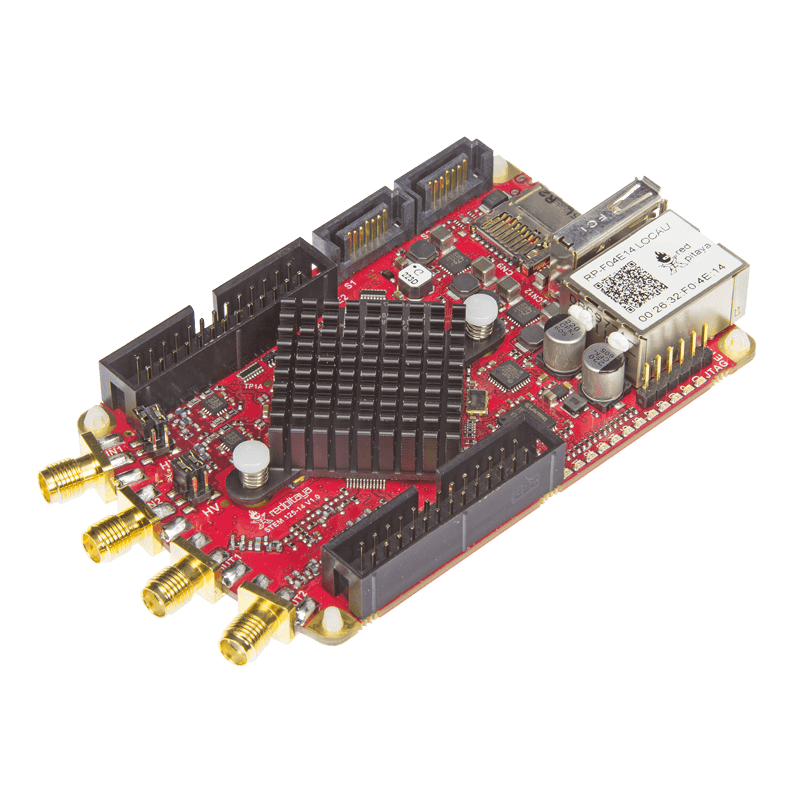
\includegraphics[width=0.67\textwidth]{images/stl125/stemlab125-14-photo.png}
    \caption{Block diagram of the Red Pitaya STEMlab. Source:~\cite{pita:elektor:starterkit}}
    \label{fig:stl125:photo}
\end{figure}

\begin{figure}
    \centering
    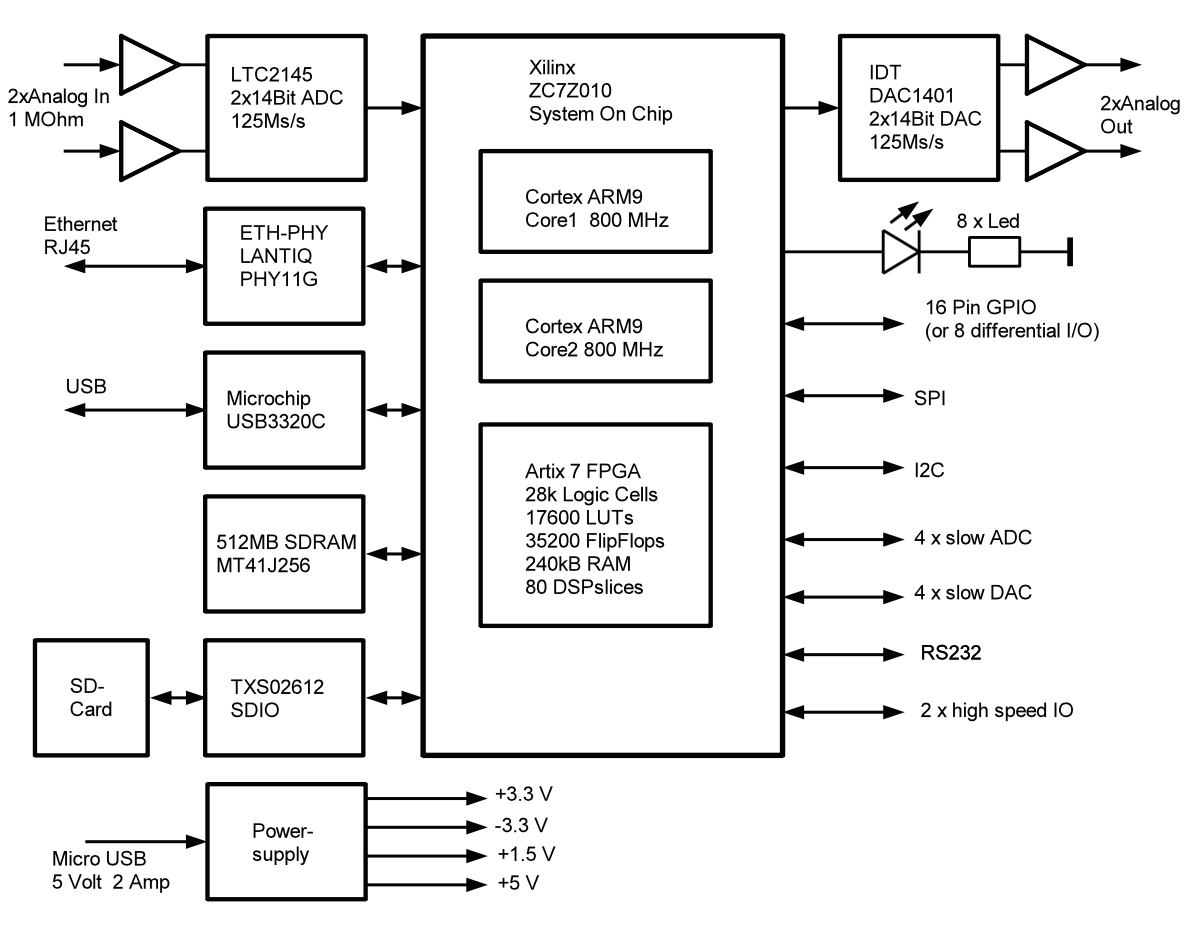
\includegraphics[width=\textwidth]{images/stl125/stemlab125.png}
    \caption{Block diagram of the Red Pitaya STEMlab. Source:~\cite{pita:ossmann}}
    \label{fig:stl125:block_diagram}
\end{figure}
%>>>


\subsection{Downsampling on the STEMlab With Stock Configuration} %<<< ------- %
\label{subsec:stl125:ds_default}
% ---------------------------------------------------------------------------- %

The  STEMlab  enables   downsampling  by  powers  of  \num{2}   in  its  stock
configuration, in a range  between $1 = 2^0$ and $65536  = 2^{16}$.  The exact
manner in which this downsampling process is performed is not easily deducible
from  public information;  the  documentation  on the  internals  of the  FPGA
codebase  is  rather  sparse. However,  work  conducted  by  our  predecessors
has  shown  that  the  STEMlab  uses   a  moving  averaging  filter  for  this
process~\cite{bucher:kuery}.

The moving averager's transfer function is
\begin{equation}
    \label{eq:moving_averager}
    H(z) = \frac{1}{N+1}\sum_{k = 0}^{N} z^{-k}.
\end{equation}
A high degree of similarity is immediately recognizable when comparing this to
the  transfer  function  of  a CIC  filter  in  Equation~\ref{eq:cic:complete}
(page~\pageref{eq:cic:complete}). Indeed, a cascade  of moving averagers would
almost yield a CIC  filter, save for the gain, which  could be easily adjusted
after the fact if needed.

A moving averager as a decimation filter is relatively cheap to implement when
using only  decimation rates of powers  of two, as  is the case for  the stock
software of the  STEMlab. The weight for each coefficient of  $z^{-k}$ will be
$\frac{1}{N+1}  =  \frac{1}{R} =  2^{-m},  m  \in \mathbb{N}_0$,  meaning  the
computations can  be performed without  multipliers by performing  a bit-shift
operations to  the right. The  primary disadvantage  which results  from these
rate reduction  factors is that the  resulting reduced sampling rates  are not
very  ``nice'' numbers,  so  to speak,  since the  incoming  sampling rate  is
\SI{125}{\MHz}, and therefore not a power of \num{2}.

Just  like a  CIC filter  by  itself, however,  a moving  averager also  makes
for  a  rather  poor  lowpass  filter, for  two  reasons: Passband  droop  and
poor  stopband   attenuation  (equivalent  to  a   single-stage  CIC  filter).
Figure~\ref{fig:stl125:moving_averager} shows  the frequency response  for the
case of  $R=8$ and  a signal  of \SI{5}{\MHz}. The  incoming sampling  rate is
\SI{125}{\MHz},  the  reduced  sampling  rate  is  $\SI{125}{\MHz}  \div  8  =
\SI{15.625}{\MHz}$. Therefore, anything  above half that frequency  is aliased
back into the region below $\SI{15.625}{\MHz} \div 2 = \SI{7.8125}{\MHz}$.  In
the case of a signal at  \SI{5}{\MHz}, this results in an aliasing attenuation
of a paltry \SI{8.06}{\dB}. Combined with the passband droop of \SI{1.48}{\dB}
(a signal  attenuation of  almost \SI{16}{\percent})  at that  frequency, this
makes for a  margin of a mere \SI{6.58}{\dB} between  the signal's attenuation
and the aliasing attenuation!

\begin{figure}
    \centering
    \newcommand*\freqzFileMAA{images/stl125/movingAveragerPBAliasingComplete.csv}
\newcommand*\freqzFileMAB{images/stl125/movingAveragerPBAliasingNull1Left.csv}
\newcommand*\freqzFileMAC{images/stl125/movingAveragerPBAliasingNull1Right.csv}
\newcommand*\freqzFileMAD{images/stl125/movingAveragerPBAliasingNull2Left.csv}
\newcommand*\freqzFileMAE{images/stl125/movingAveragerPBAliasingNull2Right.csv}
\newcommand*\freqzFileMAF{images/stl125/movingAveragerPBAliasingNull3Left.csv}
\newcommand*\freqzFileMAG{images/stl125/movingAveragerPBAliasingNull3Right.csv}
\newcommand*\freqzFileMAH{images/stl125/movingAveragerPBAliasingNull4Left.csv}
\pgfplotstableread[col sep=comma]{\freqzFileMAA}\freqzTableMAA
\pgfplotstableread[col sep=comma]{\freqzFileMAB}\freqzTableMAB
\pgfplotstableread[col sep=comma]{\freqzFileMAC}\freqzTableMAC
\pgfplotstableread[col sep=comma]{\freqzFileMAD}\freqzTableMAD
\pgfplotstableread[col sep=comma]{\freqzFileMAE}\freqzTableMAE
\pgfplotstableread[col sep=comma]{\freqzFileMAF}\freqzTableMAF
\pgfplotstableread[col sep=comma]{\freqzFileMAG}\freqzTableMAG
\pgfplotstableread[col sep=comma]{\freqzFileMAH}\freqzTableMAH
\begin{tikzpicture}
     \pgfplotsset{every axis/.style={
            height=140mm,
            width=\textwidth,
            grid=none,
            y filter/.code={\pgfmathparse{20*log10(\pgfmathresult))}},
            x filter/.code={\pgfmathparse{\pgfmathresult / 3.141592654}},
            x SI prefix=mega,
            x unit=\si{Hz},
            xticklabel style={font=\footnotesize},
            y unit=\si{dB},
            xlabel=Frequency,
            ylabel=Magnitude,
            xticklabel style={rotate=90},
            xmajorgrids=true,
        },
    }
    \begin{axis}[
            title=Passband Aliasing for Moving Averager,
            at = {(0,0)},
            xmin=0.001,
            xmax=1,
            ymin=-60,
            ymax=5,
            xtick={
                0,
                0.08,
                0.125,
                0.25,
                1%
            },
            xticklabels={%
                $0$,
                $f_\mathrm{signal} = \SI{5}{\MHz}$,
                $f_\mathrm{s,low}/2  = \SI{7.8125}{\MHz}$,
                $f_\mathrm{s,low}  = \SI{15.625}{\MHz}$,
                $f_\mathrm{s,high}/2 = \SI{62.5}{\MHz}$%
            },
            ytick={
                0,
                -20,
                -40,
                -60%
            },
        ]
        % Aliasing rectangles
        \fill[q0,opacity=0.20] ($(0.25*0.75,     -8.0571)$) rectangle ($(0.25*1.00,-60)$);
        \fill[q1,opacity=0.20] ($(0.25*1.00,     -8.0571)$) rectangle ($(0.25*1.25,-60)$);
        \fill[q2,opacity=0.20] ($(0.50-0.25*0.25,-8.0571)$) rectangle ($(0.50+0.25*0.00,-60)$);
        \fill[q3,opacity=0.20] ($(0.50-0.25*0.00,-8.0571)$) rectangle ($(0.50+0.25*0.25,-60)$);
        \fill[q4,opacity=0.20] ($(0.75-0.25*0.25,-8.0571)$) rectangle ($(0.75+0.25*0.00,-60)$);
        \fill[q5,opacity=0.20] ($(0.75-0.25*0.00,-8.0571)$) rectangle ($(0.75+0.25*0.25,-60)$);
        \fill[q6,opacity=0.20] ($(1.00-0.25*0.25,-8.0571)$) rectangle ($(1.00+0.25*0.00,-60)$);

        % Signal Frequency
        \draw[very thick,q5] (0.08,-60) -- (0.08,5);

        % Matlab results (copied by hand from movingAverager.m's output
        % aliasing_max_db         = -8.057121813367473 
        % passband_droop_db       = -1.475566945544402 
        % aliasing_attenuation_db =  6.581554867823072
        \draw (0, 0)      -- (0.47, 0);
        \draw (0,-1.4756) -- (0.47,-1.4756);
        \draw (0,-8.0571) -- (0.35,-8.0571);
        \draw[latex-latex] (0.34,-1.4756) -- (0.34,-8.0571);
        \draw[-latex]      (0.46, 0.5) -- (0.46, 0);
        \draw[-latex]      (0.46,-2)   -- (0.46,-1.4756);
        \draw              (0.46,0)    -- (0.46,-1.4756);
        \node[anchor=east] 
            at (0.825,-0.735)
            {\footnotesize passband droop at $f_\mathrm{signal}$: \SI{1.48}{\dB}};
        \node[anchor=east] 
            at (0.825,-4.9914) 
            {\footnotesize signal to aliasing attenuation at $f_\mathrm{signal}$: \SI{6.58}{\dB}};

        \addplot[very thick,da1,-] table[x=w, y=abs(H)] \freqzTableMAA;
        \addplot[line cap=round,very thick,q0,-] table[x=w, y=abs(H)] \freqzTableMAB;
        \addplot[line cap=round,very thick,q1,-] table[x=w, y=abs(H)] \freqzTableMAC;
        \addplot[line cap=round,very thick,q2,-] table[x=w, y=abs(H)] \freqzTableMAD;
        \addplot[line cap=round,very thick,q3,-] table[x=w, y=abs(H)] \freqzTableMAE;
        \addplot[line cap=round,very thick,q4,-] table[x=w, y=abs(H)] \freqzTableMAF;
        \addplot[line cap=round,very thick,q5,-] table[x=w, y=abs(H)] \freqzTableMAG;
        \addplot[line cap=round,very thick,q6,-] table[x=w, y=abs(H)] \freqzTableMAH;
    \end{axis}
\end{tikzpicture}

    \caption{%
        Frequency  response, passband  droop  and aliasing  attenuation for  a
        moving  average  filter  of  order  \num{7}  for  a  decimation  by  a
        factor of \num{8}. The incoming  sampling frequency is \SI{125}{\MHz},
        the  outgoing sampling  frequency is  \SI{15.625}{\MHz}, the  measured
        signal  has   a  frequency   of  \SI{5}{MHz}.%
    }
    \label{fig:stl125:moving_averager}
\end{figure}

As  a benchmark  for  or  own solution,  we  will  use measurements  conducted
by  our  predecessors  with  the  STEMlab's  stock  configuration,  listed  in
Table~\ref{tab:stl125:measurements_bucher_kuery}. The   measurements  do   not
actually  suggest  a very  bad  performance  of  the filter. This  is  because
they   were   conducted   at  specific   harmonic   frequencies. The   primary
issue  with  a   moving  averager  is  less  SNR   for  specific  frequencies,
but  aliasing  when  measuring  a  non-harmonic  signal  which  has  frequency
components above  $f_\mathrm{s,low}/2$. In that case, the  considerations from
Figure~\ref{fig:stl125:moving_averager}  become crucial  to understanding  the
aliasing issue.  This behavior was also confirmed in~\cite{bucher:kuery}.  Our
primary aim  is therefore more  to reduce  these aliasing effects  rather than
purely trying to improve SNR for specific single frequencies.

\begin{table}
    \centering
    \caption{%
        Measurement results  for STEMlab  125-14 from~\cite{bucher:kuery}. SNR
        was  determined for  a  specific harmonic  frequency  signal for  each
        sampling rate.%
    }
    \label{tab:stl125:measurements_bucher_kuery}
    \begin{tabular}{>{$}r<{$}>{$}r<{$}>{$}r<{$}SSS}
        \toprule
        R      &   &       & {$f_\mathrm{s,low}$ (\si{\kHz})} & {$f_\mathrm{signal}$ (\si{\kHz})} & SNR \\
        \midrule
        2^0    & = &     1 & 125000     & 10000   & \SI{62.8}{\dB} \\
        2^3    & = &     8 &  15625     &  5000   & \SI{69.8}{\dB} \\
        2^6    & = &    64 &   1953     &   500   & \SI{76.0}{\dB} \\
        2^{10} & = &  1024 &    122.1   &    40   & \SI{76.4}{\dB} \\
        2^{13} & = &  8192 &     15.26  &     5   & \SI{82.4}{\dB} \\
        2^{16} & = & 65536 &      1.907 &     0.5 & \SI{83.5}{\dB} \\
        \bottomrule
    \end{tabular}
\end{table}

In conclusion, we can formulate three main objectives:
\begin{itemize}
    \item
        Reduce  aliasing   of  out-of-range  frequency  components   into  the
        passband.
    \item
        Improve SNR.
    \item
        Have a nicer set of reduced sampling rates.
\end{itemize}

%>>>

%>>>


\section{Possible Solutions} % <<< ------------------------------------------- %
\label{sec:mission:possible_solutions}
% ---------------------------------------------------------------------------- %

Based on the  previous section, it is clear that  the downsampling filter from
the  STEMlab's  stock  configuration  must  be  replaced  if  better  aliasing
attenuation is  to be attained. Furthermore,  since a new filtering  system is
being implemented  anyway, one may wish  to change the rate  change factors in
order to achieve  a set of nicer-looking reduced  sampling rates. The question
now becomes: \emph{How}?

Problematic is that  as of spring 2017,  the official code by  Red Pitaya base
has been  split into  two: There is  a new  development branch  bringing major
changes, while  the old code  (which has been  used in the  projects preceding
this one) is no longer being maintained, as explained by one of the developers
(see~\cite{pita:github:issue:huesser:jeras}):
\begin{quote}
    Current  development  is done  on  the  \code{mercury} branch  on  the
    FPGA  subproject of  the same  name.  The  code is  still under  heavy
    development and  not stable. All  other FPGA  subprojects will  not be
    developed further.
\end{quote}

Essentially, this presents us with three options on how to proceed:
\begin{itemize}
    \item
        Use  the old  Red Pitaya  codebase,  and implement  our new  filtering
        system based  on that.
    \item
        Use the new  Red Pitaya codebase. Due to this  codebase being unstable
        according to the developers themselves as of the time of this project,
        we consider this to be an unviable option.
    \item
        Use an alternative  ecosystem, either by a third party  (if one can be
        found) or developed by ourselves.
\end{itemize}
In   order    to   have    a   somewhat    objective   measure    to   compare
the   first   and   last   option,    a   decision   matrix   is   used;   see
table~\ref{tab:decision_matrix:pitaya_vs_own}. In  the  following  paragraphs,
the criteria and weighings in the  table are elaborated upon. The table uses a
scale of  \num{1} through \num{6},  with \num{1}  being the worst  and \num{6}
being the best score. At the end, totals are tallied and compared.

\paragraph{Reliance  upon others:} Using  the  existing  Red Pitaya  ecosystem
would also  couple us  to any problems  inherent to that  platform and  to the
solutions developed by preceding projects based on it. Any bugs encountered in
the Red Pitaya ecosystem would either  require a bugfix by the manufacturer or
a workaround on our part. Since the old Red Pitaya codebase is no longer being
maintained by  the developers, bugfixes will  not be available, leaving  us to
clean  up  any potential  issues  inherent  to  the  codebase. If we  were  to
implement our  own solution instead, we  would be less reliant  upon others to
fix  any inherent  problems to  the code. These  factors lead  us to  give the
existing codebase a rather weak rating of, compared to a strong rating for the
choice of pursuing our own solution.

\paragraph{Flexibility:} Obviously, implementing our own  system would give us
much higher flexibility  than using the existing ecosystem. The  only two true
limitations would  be the  time and  hardware resources  available to  us. the
official codebase would limit us to its capabilities. Adding new functionality
to the existing codebase would be possible, but adapting software for purposes
for which  it was  not originally  intended does tend  to be  a time-consuming
procedure  in our  experience.  Therefore,  the option  of developing  our own
solution wins out again here.

\paragraph{Complexity  of  complete  system:} This  refers  not  just  to  the
complexity  of  the  components  we  work  on,  but  of  the  entire  platform
and  ecosystem. As  anyone who  bothers  to  peruse  the Red  Pitaya  codebase
(\cite{pita:github}) can  dedude, it is  a large ecosystem with  many features
and capabilities, most of which are not relevant to our needs. A custom system
developed for the specific needs of this project would be much leaner and have
fewer points of failure.

\paragraph{Labor  costs:} Here  is where  using  the  existing codebase  would
be  beneficial  in our  view. While  understanding  its inner  workings  would
doubtlessly be required and take a significant amount of time (particularly in
view  of  the sparse  documentation  at  this  point  in time),  developing  a
completely  new system  more or  less from  scratch would  be a  much costlier
undertaking in terms of required man-hours, we estimate.

\paragraph{Chances of success:} Basing our work on the existing codebase would
unburden  us  of  the  legwork  needed  to  get  basic  functionality  up  and
running. We could exchange  the filter components of the  existing system with
our own, but leave most of the remaining system untouched. The challenge would
be to understand the  system well enough to do this.   Building our own system
would require re-implementing more components  of the Red Pitaya platform than
just the filters. As each additional task  increases the risk of failure, this
is not without  risk to the overall success. Overall, we  consider this factor
to be roughly even between the two choices.

\paragraph{Robustness  of third-party  components:} This criterion  takes into
account our assessment  of the reliability and dependability  of any component
we use which  is not developed by ourselves, along  with its documentation and
manufacturer  support. In the  case of  the  Red Pitaya  codebase, this  would
primarily  comprise the  codebase  itself as  well as  any  components for  it
developed  by other  parties. If  we were  to develop  our  own solution,  the
building blocks would primarily be the  Xilinx toolchain and libraries for the
SoC.

Because  the  Red  Pitaya  codebase  is rather  large,  not  well  documented,
comparatively new and no longer being maintained, and the company is small and
more likely  to be  stretched thin, we  do not score  the Red  Pitaya codebase
highly here. The  Xilinx toolchain and  FPGA libraries, while  undoubtedly not
without bugs,  have had  a lot  of time to  mature on  the other  hand.  Also,
Xilinx is a big company with vast resources, so any bugs which are encountered
in  their products  are more  likely to  be addressed  in our  view. For these
reasons, we score  developing our own solution higher than  using the existing
cosebase.

\paragraph{Reparability:} If any issues are found in the resulting product, we
are more likely to  be able to fix them if it is  our own codebase rather than
that by a third party.

\paragraph{Long-term viability:} Developing  our own  solution would  allow us
(or anyone  else wishing  to base their  work off of  ours) to  address future
needs relatively  easily. Using the  existing code base  would make  this more
difficult in our view.

\paragraph{Conclusion:} Developing our  own solution does carry  a significant
risk  and is  likely  to require  more  work than  basing  our application  on
existing  work.   But in  light  of  the  mentioned  drawbacks of  the  latter
approach, we still find that it is  the preferable approach and is more likely
to lead to a successful outcome.


\begin{table}
    \centering
    \caption{%
        Decision   matrix   comparing   the   usage  of   the   existing   Red
        Pitaya   ecosystem  against   building   our   own  data   acquisition
        system. Weighing: Scale  of \num{1}  (worst)  to \num{6}  (best). More
        total points is better.%
    }
    \label{tab:decision_matrix:pitaya_vs_own}
    \begin{tabular}{>{\raggedright}p{80mm}SS}
        \toprule
        & RP & Custom \\
        \midrule
        reliance on others &
        2 & 5 \\

        flexibility &
        2 & 5 \\

        complexity of complete system &
        1 & 4 \\

        labor costs &
        4 & 2 \\

        chances of success &
        4 & 4 \\

        available documentation for used building blocks &
        3 & 5 \\

        robustness of third-party components &
        2 & 5 \\

        reparability &
        2 & 5 \\

        long-term viability&
        2 & 4 \\
        \midrule
        Total & 21 & 37 \\
        \bottomrule
    \end{tabular}
\end{table}

%>>>


\section{Concept} % <<< ------------------------------------------------------ %
\label{sec:mission:concept}
% ---------------------------------------------------------------------------- %

Having concluded that  we shall develop our own solution  from scratch, we can
now  develop  a  concept  for  how  that solution  will  look.   On  the  most
fundamental level, it will require the following components:
\begin{itemize}
    \item
        a custom FPGA firmare for data acquisition and filtering
    \item
        a new scope application for data visualization
    \item
        an interfacing layer between the FPGA and the scope
    \item
        optionally, the possibility to connect to other applications like Matlab
\end{itemize}
The   following   sections   elaborates   on  the   general   shape   of   our
solution. Chapters~\ref{ch:fpga}  through~\ref{ch:graphical_front_end} explain
the components  in detail, while Chapter~\ref{ch:filter_design}  documents the
filter design process, which is rather separate from the firmware and software
and therefore a dedicated chapter.


\subsection{FPGA Components} % <<< ------------------------------------------- %
\label{subsec:concept:fpga_components}
% ---------------------------------------------------------------------------- %

On the most abstract level, the FPGA part of our system will need to be able to
\begin{itemize}\tightlist
    \item
        acquire data from the ADC,
    \item
        decimate and filter it,
    \item
        and pass it on for further processing.
\end{itemize}

Due to the  platform's open nature, there exist some  projects for the STEMlab
by parties other than Red Pitaya  themselves. One of these is \emph{Red Pitaya
Notes} by  Pavel Denim, available  at~\cite{pita:github:pitaya-notes}. As part
of that  project, Mr. Denim  has implemented  an ADC core  for the  FPGA which
acquires  data from  the ADC's  two  channels and  passes  it on  via an  AXI4
streaming interface\footnotemark.
\footnotetext{%
    Xilinx's proprietary general-purpose interconnect for moving large amounts
    of data around an FPGA
}
Since   this   project  is   open-source   and   has  a   permissive   license
(MIT   license~\cite{licenses:mit},   template   text    can   be   found   in
Appendix~\ref{sec:mit_license} on page~\pageref{sec:mit_license}) and fulfills
our  main technical  requirement (easily  interfaceable),  it is  used in  our
project to interface the FPGA with the ADC.

For filtering,  one can either  implement custom filter topologies  from basic
FPGA building blocks (adders, multipliers, etc.), write completely custom VHDL
or Verilog code, or use ready-made blocks, if available.  Xilinx provides such
FPGA  blocks for  FIR  and CIC  filters,  both of  which  come with  excellent
documentation  (see~\cite{xilinx:cic-compiler} and~\cite{xilinx:fir-compiler},
respectively).  In  order to avoid  re-inventing the  wheel, so to  speak, and
take advantage of  some of the advanced features offered  by these two blocks,
we use these two building blocks in our design.

Interfacing  between the  FPGA  and  the outside  world  requires a  component
which  can take  data  from the  filters  and  hand it  off  to the  GNU/Linux
running  on the  ARM cores. Additionally,  the user  must be  able to  trigger
measurements   from  the   operating  system. Luckily,   Mr. H\"usser  already
developed  such  a  data  logging  core  for  a  Xilinx  FPGA  in  an  earlier
project~\cite{pita:github:huesser:zynq-logger},  which  comes  with  a  kernel
module to interface  with GNU/Linux. With some minor adaption  work, this core
should suit our needs nicely.

The  last  component needed  for  the  FPGA is  a  control  logic to  set  the
decimation  rate  and  enable  or  disable specific  components  of  the  data
processing  chain. This  should  be   fairly  straightforward,  and   will  be
implemented by ourselves as a custom block.

In summary, the concept for the FPGA data processing system looks as follows:
\begin{itemize}\tightlist
    \item
        The ADC is accessed via Pavel Denim's ADC core.
    \item
        Filtering the data is conducted with Xilinx's CIC and FIR compilers.
    \item
        For interfacing  with GNU/Linux,  Mr. H\"usser's data logging  core is
        used.
    \item
        A custom control logic configures the data processing chain on-the-fly
        through user input.
\end{itemize}
%>>>

\subsection{Interfacing Layer} % <<< ----------------------------------------- %
\label{subsec:concept:interfacing_layer}
% ---------------------------------------------------------------------------- %

The interfacing layer is responsible for  sending the data from the STEMlab to
the  user application  running  on  a computer. This  is  done  via a  Gigabit
Ethernet connection. As  is easily apparent,  this connection is far  too slow
for  moving all  data off  the device  which is  generated by  the ADC  (about
\SI{3.7}{\gibi\byte\per\second}), hence  the need for decimation  (among other
reasons).

For the  interfacing layer,  a server  application is run  on the  STEMlab, to
which a  client can connect. The  server takes  data from the  logger's kernel
module,  processes  and packages  it  as  necessary,  and  sends it  out  over
Ethernet.  The application is documented in detail in Chapter~\ref{ch:server},
starting on page~\pageref{ch:server}.

TODO: More blabla?
%>>>

\subsection{Scope} % <<< ----------------------------------------------------- %
\label{subsec:concept:scope}
% ---------------------------------------------------------------------------- %

The scope is the main interface between the end user and the STEMlab in our
system. Through it, data can be visualized and analyzed in both the time and
frequency domain.

In  order  to  ensure  maximum   portability,  the  scope  is  implemented  as
a   web   application   rather   than   a   cusom   binary. This   allows   it
to   function   on   any   operating   system   with   a   reasonably   modern
browser. A  through  documentation  of  its  capabilities  and  implementation
is   available    in   Chapter~\ref{ch:graphical_front_end},    beginning   on
page~\ref{ch:graphical_front_end}.

TODO: more blabla?
%>>>


%>>>
%>>>
%^^A vim: foldenable foldcolumn=4 foldmethod=marker foldmarker=<<<,>>>

% ------------------------------------------------------------------------->>> %
% <<< ---------------------------------------------------------- FILTER DESIGN %
\chapter{Filter Design} % <<< ------------------------------------------------ %
\label{ch:filter_design}
% ---------------------------------------------------------------------------- %

Some    key    points    underlying     the    theory    of    filters    have
been   treated   in  Chapter~\ref{ch:analog-to-digital_data_aquisition},   and
Chapter~\ref{ch:mission}  defines  the  overall objectives  of  this  project;
implementing a  custom filtering system  on the FPGA among  them. This chapter
will now develop a concrete concept for that filtering system, address some of
the issues encountered when moving from  the theory of filters to the practice
of designing them, and then define the  actual filters which are to be used on
the FPGA. The implementation of those filters  on the FPGA is addressed in the
following chapter, beginning on page~\pageref{ch:fpga}.


\section{Requirements} % <<< ------------------------------------------------- %
\label{sec:requirements}
% ---------------------------------------------------------------------------- %

The overarching  objective is downsampling the  signal coming out of  the ADC.
This  section will  derive  upper  and lower  boundaries  for the  downsampled
frequency range, and then define the specific downsampling ratios to be used.

The total data rate from the ADC is
\sisetup{inter-unit-product = \ensuremath { { } \cdot { } }}
\begin{alignat}{4}
    S                  &= \SI{125}{\mega\sample\per\second}                                  & & \nonumber  \\
    N_\mathrm{ch}      &= 2                                                                  & & \nonumber  \\
    B_\mathrm{ch}      &= \SI{14}{\bit\per\sample}                                           & & \nonumber  \\
    B_\mathrm{ch,pad}  &= \SI{2}{\bit\per\sample}                                            & & \nonumber  \\
    B_\mathrm{ADC}     &= N_\mathrm{ch} \cdot \left(B_\mathrm{ch} + B_\mathrm{ch,pad}\right) \,\,&=&\,\, \SI{32}{\bit\per\sample} \nonumber \\
    R                  &= S \cdot B_\mathrm{ADC}                                             \,\,&=&\,\, \SI{4}{\giga\bit\per\second} \label{eq:adc_data_rate}
\end{alignat}
\begin{conditions}
    S                  & sampling rate                         \\
    N_\mathrm{ch}      & number of channels                    \\
    B_\mathrm{ch}      & channel width                         \\
    B_\mathrm{ch,pad}  & padding per channel                   \\
    B_\mathrm{ADC}     & total width of bit stream out of ADC  \\
    R                  & total data rate out of ADC in bit     \\
\end{conditions}
%\sisetup{inter-unit-product = \,}

The   upper   boundary  for   the   resulting   sampling   rate  is   set   by
the   STEMlab's   network    connection,   which   has   a    data   rate   of
\SI{1000}{\mega\bit\per\second}. A downsampling factor of  at least \num{4} is
therefore required  for real-time data transmission. Because  \num{125} is not
divisible by \num{4}, a factor of  \num{5} is chosen instead. This makes for a
resulting data  rate of  \SI{800}{\mega\bit\per\second}, which should  also be
easily sufficient for protocol overhead.

On the lower end  of the spectrum, the system should still  be able to process
audio  signals. Common  sampling  frequencies for  audio  are  \SI{44.1}{\kHz}
for  audio CDs,  and \SI{48}{\kHz}  for  the audio  component of  audio-visual
applications. Neither  of these  frequencies  fit  nicely into  \SI{125}{\MHz}
(requiring large  prime factor  for the  rate change),  so the  lower boundary
is  specified  as \SI{50}{\kHz},  corresponding  to  a downsampling  ratio  of
\num{2500}.

To cover  additional use cases,  some additional sampling  frequencies between
these   two  boundaries   are  specified. Table~\ref{tab:ratio_decompositions}
contains  the   complete  list   of  downsampling   ratios,  along   with  the
corresponding sampling frequencies.

\begin{table}
    \centering
    \caption[Downsampling Ratios, Decompositions, and Target Frequencies]{
        The  chosen downsampling  ratios, their  prime factor  decompositions,
        the  downsampling ratios  distribet across  stages, and  the resultant
        sampling rates%
    }
    \label{tab:ratio_decompositions}
    \begin{tabular}{S >{$}r<{$} >{$}l<{$} S}
        \toprule
        {R}  & \text{Decomposition}                                                 & \text{Stages}                                 & {$f_s$ (\si{\kHz})} \\
        \midrule
           5 &  5                                                   = 5^1           &   5                                           & 25000               \\
          25 &  5 \cdot 5                                           = 5^2           &   5 \rightarrow 5                             &  5000               \\
         125 &  5 \cdot 5 \cdot 5                                   = 5^3           &  25 \rightarrow 5                             &  1000               \\
         625 &  5 \cdot 5 \cdot 5 \cdot 5 \cdot 5                   = 5^4           &  25 \rightarrow 5 \rightarrow 5               &   200               \\
        1250 &  2 \cdot 5 \cdot 5 \cdot 5 \cdot 5 \cdot 5           = 2^1 \cdot 5^4 & 125 \rightarrow 5 \rightarrow 2               &   100               \\
        2500 &  2 \cdot 2 \cdot 5 \cdot 5 \cdot 5 \cdot 5 \cdot 5   = 2^1 \cdot 5^4 & 125 \rightarrow 5 \rightarrow 2 \rightarrow 2 &    50               \\
        \bottomrule
    \end{tabular}
\end{table}


%>>>


\section{Cascade Concept} % <<< ---------------------------------------------- %
\label{sec:cascade_concept}
% ---------------------------------------------------------------------------- %

Based  on the  downsampling factors  from Table~\ref{tab:downsampling_ratios},
this section  presents the  general concept for  the cascades  which implement
those rate changes.

As  discussed  in  Section~\ref{sec:multi_stage_filter_designs},  implementing
high   downsampling   ratios   in   a    single   stage   is   generally   not
a   sound   design   choice. Consequently,  the   downsampling   ratios   from
Table~\ref{tab:downsampling_ratios} must  be decomposed into  smaller factors,
which can then be distributed along a chain. These factors must fulfill the
following criteria:
\begin{itemize}\tightlist
    \item
        Filters  for  different stages  should  be  re-usable across  multiple
        downsampling ratios  in order  to save resources. Rate  change factors
        which  are  common  to  multiple rate  change  factors  are  therefore
        preferred.
    \item
        The factors for the individual stages  should be large enough to be of
        utility,  but small  enough so  as not  to make  the resulting  filter
        impractically narrow.
\end{itemize}
CIC  filters  are  well-suited  for  large   rate  changes,  but  are  not  an
optimal solution  for smaller  ones. As an  example of  a low-rate  change CIC
filter,  Figure~\ref{fig:cic_simu:freqz} on  page~\pageref{fig:cic_simu:freqz}
in  Appendix~\ref{sec:app:cic_simu}  shows the  frequency  response  of a  CIC
filter with a rate change of \num{2}.

Based on that observation, it is reasonable to implement the lower rate change
factors without CIC  filters, while using CIC filters as  the first element in
the filter  chain for  the higher rate  changes. This allows  taking advantage
of  the CIC  filter's  high computational  efficiency  for large  downsampling
rates,  while still  having good  frequency  response behavior  for the  lower
rate  changes. Table~\ref{tab:ratio_decompositions}  shows  the  prime  factor
decomposition for the overall rate changes,  as well as the factors chosen for
the individual filter chain stages.

Other choices are of course possible. Particularly in the case of $R=625$, one
may  choose  to implement  a  chain  of $125  \rightarrow  5$  instead of  $25
\rightarrow  5 \rightarrow  5$.   The  two implementations  as  they would  be
in  the  final  design  are compared  in  Figure~\ref{fig:dec625_variants}  on
\pageref{fig:dec625_variants} in Appendix~\ref{sec:dec625_variants}. While the
$125 \rightarrow 5$ chain would offer better stopband attunation behavior over
certain frequency  ranges and  therefore improved SNR,  the $25  \rightarrow 5
\rightarrow 5$ chain  offers the advantage that if the  design is ever changed
and only  the higher sampling rates  are implemented (removing the  chains for
$R=1250$ and $R=2500$), it can re-use the elements from the higher chains. The
$25 \rightarrow  5 \rightarrow 5$  chain is  therefore chosen.
%>>>

\section{Filter Specifications} % <<< ---------------------------------------- %
\label{sec:fdesign:filter_specifications}
% ---------------------------------------------------------------------------- %

Continuing  from Table~\ref{tab:ratio_decompositions},  this section  presents
the  concept for  the cascades  which  are used  in our  design. Specifically,
requirements and constraints for the  filters in those cascades are specified.
For this purpose, it is no longer sufficient to merely consider the filters in
the mathematical  sense; resource  usage on  the hardware  must be  taken into
account.

The hardware places two main contrainst on the design:
\begin{itemize}\tightlist
    \item
        Number of available LUTs: \num{17600}
    \item
        Number of available DSP slices: \num{80}
\end{itemize}
The number  of LUTs  is relevant  for storage  (filter coefficients),  the CIC
filters\footnote{%
    The CIC compiler block by Xilinx can be configured to utilize LUTs instead
    of DSP  slices for  its computations. The  FIR compiler  can only  use DSP
    slices for its computations.%
},
the  rest of  the processing  system, and  control logic. The  DSP slices  can
therefore  be  reserved  for  the  FIR filters. Because  the  device  has  two
channels, only 40 slices may be used per channel.

In order to have  a realistic gauge for resource usage of  the FIR filters, it
is  necessary to  keep  in  mind the  two  factors  which primarily  influence
resource usage:
\begin{itemize}\tightlist
    \item
        the sampling frequency at which the filter runs (its incoming sampling
        rate),
    \item
         and the number of coefficients, and therefore, adders and multipliers.
\end{itemize}
It is  therefore important to  know which filters in  the design run  at which
sampling  rates. For this  to  be possible,  a concept  of  the six  different
filter  chains   is  needed. Based   on  Table~\ref{tab:ratio_decompositions},
Figure~\ref{fig:fdesign:chain_concept} depicts  that concept. It  includes all
the required  filters of the  design, including  the compensators for  the CIC
filters. Note that  one of  the compensators  is itself  used as  a decimation
filter in the case of the $R=1250$ and $R=2500$ chains.

\begin{figure}
    \centering
    \tikzsetnextfilename{chainConcepts}
\begin{tikzpicture}[
        node distance=5mm,
        every node/.style={
            font=\ttfamily,
            rounded corners=1mm,
            text centered,
            minimum width=4em,
            minimum height=3.5ex,
            text height=1.5ex,
            text depth=0.25ex,
        },
        5steep/.style={
            draw=sqC,
            fill=sq5,
        },
        5flat/.style={
            draw=sq9,
            fill=sq3,
        },
        2steep/.style={
            draw=dv-7,
            fill=dv-3,
        },
        2flat/.style={
            draw=dv-5,
            fill=dv-1,
        },
        cic25/.style={
            draw=q4,
            fill=q4!80!white,
        },
        cic125/.style={
            draw=q5,
            fill=q5!80!white,
        },
        cfir25/.style={
            draw=q4,
            fill=q4!50!white,
        },
        cfir125/.style={
            draw=q5,
            fill=q5!50!white,
        },
        compressor/.style={
            draw=br0,
            fill=br1,
            minimum width=1em,
        },
    ]
    \node[5steep]                      (5steep5) at (0,0) {5steep};
    \node[compressor,right=of 5steep5] (5compr5a)         {$5\downarrow$};
    \coordinate[left=of 5steep5]   (in5);
    \coordinate[right=of 5compr5a] (out5);
    \draw[-latex] (in5)      -- (5steep5);
    \draw[-latex] (5steep5)  -- (5compr5a);
    \draw[-latex] (5compr5a) -- (out5);

    \node[5flat   ,below=of 5steep5]    (5flat25)   {5flat};
    \node[compressor,right=of 5flat25]  (5compr25a) {$5\downarrow$};
    \node[5steep  ,right=of 5compr25a]  (5steep25)  {5steep};
    \node[compressor,right=of 5steep25] (5compr25b) {$5\downarrow$};
    \coordinate[left=of 5flat25]    (in25);
    \coordinate[right=of 5compr25b] (out25);
    \draw[-latex] (in25)      -- (5flat25);
    \draw[-latex] (5flat25)   -- (5compr25a);
    \draw[-latex] (5compr25a) -- (5steep25);
    \draw[-latex] (5steep25)  -- (5compr25b);
    \draw[-latex] (5compr25b) -- (out25);

    \node[cic25   ,below=of 5flat25]     (25cic125)   {CIC25};
    \node[compressor,right=of 25cic125]  (5compr125a) {$25\downarrow$};
    \node[cfir25  ,right=of 5compr125a]  (1cfir125)   {CFIR25};
    \node[5steep  ,right=of 1cfir125]    (5steep125)  {5steep};
    \node[compressor,right=of 5steep125] (5compr125b) {$5\downarrow$};
    \coordinate[left=of 25cic125]    (in125);
    \coordinate[right=of 5compr125b] (out125);
    \draw[-latex] (in125)      -- (25cic125);
    \draw[-latex] (25cic125)   -- (5compr125a);
    \draw[-latex] (5compr125a) -- (1cfir125);
    \draw[-latex] (1cfir125)   -- (5steep125);
    \draw[-latex] (5steep125)  -- (5compr125b);
    \draw[-latex] (5compr125b) -- (out125);

    \node[cic25   ,below=of 25cic125]    (25cic625)    {CIC25};
    \node[compressor,right=of 25cic625]  (25compr625a) {$25\downarrow$};
    \node[cfir25  ,right=of 25compr625a] (1cfir625)    {CFIR25};
    \node[5flat   ,right=of 1cfir625]    (5flat625)    {5flat};
    \node[compressor,right=of 5flat625]  (5compr625b)  {$5\downarrow$};
    \node[5steep  ,right=of 5compr625b]  (5steep625)   {5steep};
    \node[compressor,right=of 5steep625] (5compr625c)  {$5\downarrow$};
    \coordinate[left=of 25cic625]    (in625);
    \coordinate[right=of 5compr625c] (out625);
    \draw[-latex] (in625)      -- (25cic625);
    \draw[-latex] (25cic625)   -- (25compr625a);
    \draw[-latex] (25compr625a) -- (1cfir625);
    \draw[-latex] (1cfir625)   -- (5flat625);
    \draw[-latex] (5flat625)   -- (5compr625b);
    \draw[-latex] (5compr625b) -- (5steep625);
    \draw[-latex] (5steep625)  -- (5compr625c);
    \draw[-latex] (5compr625c) -- (out625);

    \node[cic125  ,below=of 25cic625]      (125cic1250)    {CIC125};
    \node[compressor,right=of 125cic1250]  (125compr1250a) {$125\downarrow$};
    \node[cfir125 ,right=of 125compr1250a] (5cfir1250)     {CFIR125};
    \node[compressor,right=of 5cfir1250]   (5compr1250b)   {$5\downarrow$};
    \node[2steep  ,right=of 5compr1250b]   (2steep1250)    {2steep};
    \node[compressor,right=of 2steep1250]  (2compr1250c)   {$2\downarrow$};
    \coordinate[left=of 125cic1250]   (in1250);
    \coordinate[right=of 2compr1250c] (out1250);
    \draw[-latex] (in1250)        -- (125cic1250);
    \draw[-latex] (125cic1250)    -- (125compr1250a);
    \draw[-latex] (125compr1250a) -- (5cfir1250);
    \draw[-latex] (5cfir1250)     -- (5compr1250b);
    \draw[-latex] (5compr1250b)   -- (2steep1250);
    \draw[-latex] (2steep1250)    -- (2compr1250c);
    \draw[-latex] (2compr1250c)   -- (out1250);

    \node[cic125 ,below=of 125cic1250]    (125cic2500)    {CIC125};
    \node[compressor,right=of 125cic2500] (125compr2500a) {$125\downarrow$};
    \node[cfir125,right=of 125compr2500a] (5cfir2500)     {CFIR125};
    \node[compressor,right=of 5cfir2500]  (5compr2500b)   {$5\downarrow$};
    \node[2steep ,right=of 5compr2500b]   (2flat2500)     {2steep}; % Not a typo
    \node[compressor,right=of 2flat2500]  (2compr2500c)   {$2\downarrow$};
    \node[2steep ,right=of 2compr2500c]   (2steep2500)    {2steep};
    \node[compressor,right=of 2steep2500] (2compr2500d)   {$2\downarrow$};
    \coordinate[left=of 125cic2500]   (in2500);
    \coordinate[right=of 2compr2500d] (out2500);
    \draw[-latex] (in2500)        -- (125cic2500);
    \draw[-latex] (125cic2500)    -- (125compr2500a);
    \draw[-latex] (125compr2500a) -- (5cfir2500);
    \draw[-latex] (5cfir2500)     -- (5compr2500b);
    \draw[-latex] (5compr2500b)   -- (2flat2500);
    \draw[-latex] (2flat2500)     -- (2compr2500c);
    \draw[-latex] (2compr2500c)   -- (2steep2500);
    \draw[-latex] (2steep2500)    -- (2compr2500d);
    \draw[-latex] (2compr2500d)   -- (out2500);
\end{tikzpicture}

    \caption[Filter Chain Concept]{The concept for the filter chains}
    \label{fig:fdesign:chain_concept}
\end{figure}

Because the final filter in a cascade  is the one which determines the overall
transition  band  (see  Section~\ref{sec:multi_stage_filter_designs}),  it  is
desirable to have maximally steep  output filters in a cascade. Therefore, the
filter \code{5steep} should be as sharp  as possible. Since that filter is not
just used as the  final stage in some cascades, but also  as the single filter
for the $R=5$ chain, it runs  at the highest sampling frequency%
\footnote{%
    It should be noted at this point  that a filter which is configured to run
    at a high  sampling rate can be re-used  as a lower stage in  a cascade in
    the Xilinx toolchain. The filter's behavior  in that case is correct, even
    when being run at a lower rate than maximally possible.%
}.
\code{5steep}  is therefore  the most  critical  filter in  terms of  resource
usage. The filter \code{5flat} also runs  at the highest sampling frequency in
the $R=25$  chain, but because it  is not the  final filter in that  chain, it
need not be as steep.

While  it is  possible to  estimate  the needed  resources of  a given  filter
design,  reliable  figures  are  best   obtained  by  way  of  experiment. The
FPGA  toolchain  might  make  optimizations   which  are  hard  to  take  into
account   when  performing   estimates  by   hand.   The   results  of   these
measurements are  available in  Appendix~\ref{sec:fir_filter_resouce_usage} on
page~\pageref{sec:fir_filter_resouce_usage}. Based on those  numbers, a filter
size  of around  \num{200}  is  determined to  be  a  reasonable boundary  for
\code{5steep}; a filter of that size uses about
TODO
DSP slices. This leaves
TODO
number  of  slices   for  the  remaining  filters   (per  channel). Of  these,
\code{5flat} is the most critical, because it  must also be able to run at the
full incoming sampling frequency. \code{2steep}  runs at a much lower sampling
rate  and can therefore be of significant size without a notable penalty in
resource usage.

Based  on  these  findings  and   the  measurements  of  the  STEMlab's  stock
configuration from  Section~\ref{subsec:stl125:ds_default}, it is  possible to
define performance specifications  for the filters without needing  to prod in
the dark,  so to  speak. The following  paragraphs explain  the considerations
which lead to  the final filter specifications. The results  are summarized in
Table~\ref{tab:filter_specs}.

\paragraph{Requirements  for   \code{5steep}:}   Based   on  the   results  of
the  moving  averager   used  in  the  STEMlab's   stock  configuration,  even
a  FIR  filter  with   moderate  performance  characteristics  should  already
offer   significant   improvements. In   order  to   achieve   notable   gains
over  the   default  configuration,   the  following  performance   goals  for
\code{5steep}   are  specified,   according  to   the  pattern   explained  in
Section~\ref{subsec:FIR_filters}:
\begin{itemize}\tightlist
    \item
        Passband ripple: better than \SI{0.25}{\dB}
    \item
        Stopband attenuation: \SI{60}{\dB} or better
    \item
        Transition band width: $0.05 \cdot f_\mathrm{s}/2$ or better
\end{itemize}
The     stopband    attenuation     criterion    is     also    applied     to
all    other     filters. Anything    else    would    be     a    waste    of
resources,   as   shown    in   Figure~\ref{fig:fdesign:cascade:ast_demo}   in
Section~\ref{sec:multi_stage_filter_designs}.

\paragraph{Requirements   for  \code{5flat}:} This   filter   need  not   have
a   drop-off  as   sharp   as   \code{5steep},  as   long   as   the  end   of
its   transition   band   does   not   overlap   with   the   first   spectral
copy  of  \code{5steep} (see  Figure~\ref{fig:fdesign:cascade:good_vs_bad}  in
Section~\ref{sec:multi_stage_filter_designs}).   However, because  it is  in a
cascade with  \code{5steep}, a sharper  requirement on its passband  ripple is
imposed,  in order  not  to worsen  overall passband  ripple  behavior of  the
cascade too much.

\paragraph{Requirements    for    \code{2steep}:} In   theory,    the    first
decimator-by-two in  the chain  for $R=2500$  could be  designed with  a wider
transition band than the one which is  being used as the last stage (hence the
designator \code{5steep}). However, because  these filters do not  have to run
at high sampling rates, the amount of DSP slices they use is very low (\num{1}
DSP slice per channel),  so the same filter can be  re-used without a resource
penalty.

TODO: halfband

\paragraph{Requirements     for     \code{CIC25}:} The     relevant     design
criteria    for   the    CIC    filter   are    its   stopband    attenuation,
its   decimation    rate,   and   the   cutoff    frequency/desired   passband
width    (see   Figure~\ref{fig:cic:freq_responses:passband:attenuation}    in
Section~\ref{subsubsec:cic:frequency_characteristics}).  The  cutoff frequency
is chosen such that it matches the  frequency band which is of interest at the
end of the filter chain  for $R=125$, i.e. $f_\mathrm{P} = f_\mathrm{s,high}/R
=  0.008$. This means  that  the passband  of  \code{CIC25} and  \code{CFIR25}
combined is too wide by a factor of \num{5} for the $R=625$ chain, but this is
of no concern because it will be cut  off by \code{5flat} as the last stage in
that  case. This allows  the  re-use of  the two  filters  across both  chains
without changing their design parameters.

\paragraph{Requirements for \code{CIC125}:} The same considerations as for the
other CIC  filter apply. The filter  and its  compensator are specified  for a
rate  change  of  \num{125}  and  \num{5} instead  of  \num{25}  and  \num{1},
respectively, and  the cutoff frequency  is set to  match the filter  chain of
$R=1250$. This makes it twice as wide as it needs to be for $R=2500$, which is
corrected by a second halfband filter.

\paragraph{Requirements     for     compensators:} The    compensators     are
specified     according    to     the    considerations     laid    out     in
Section~\ref{subsubsec:cic:compensators},   with   the    added   feature   of
\code{CIC125} also being used as a decimator.

\paragraph{Summary:} With  the  above   considerations  and  the  experimental
results for  resource usage  from Appendix~\ref{sec:fir_filter_resouce_usage},
it  is  possible  to  formulate  a complete  set  of  specifications  for  the
filters. They  are  compiled   in  Table~\ref{tab:filter_specs}.   Translating
the   specifications    from   Table~\ref{tab:filter_specs}    into   absolute
frequencies  results  in   the  values  from  Table~\label{tab:tb_widths}. The
frequency    responses    of   all    filters    and    filter   chains    are
depicted   in   Appendix~\ref{sec:filter_frequency_responses},   starting   on
page~\pageref{sec:filter_frequency_responses}.

\begin{table}
    \centering
    \caption[Summary of Filter Specifications]{
        The   target   filter   specifications. These  parameters   are  based
        both  on  the  desired  frequency   domain  behavior  of  the  filters
        as   well  as   the  feasibility   of  implementation   in  terms   of
        resource   usage. For  resource   considerations,  the   results  from
        Appendix~\ref{sec:fir_filter_resouce_usage} are used as a guideline.%
    }
    \label{tab:filter_specs}
    \newcommand*\NA{\footnotesize N/A}
    \begin{tabular}{>{\ttfamily}lSSSS}
        \toprule
        \sffamily Filter                                                          &
        {\parbox[t]{26.5mm}{Passband Edge \\ ($\times \pi \si{\radian\per\sample}$)}} &
        {\parbox[t]{26.5mm}{Stopband Edge \\ ($\times \pi \si{\radian\per\sample}$)}} &
        {\parbox[t]{26.5mm}{Passband Ripple \\ (\si{\dB})}}                           &
        {\parbox[t]{26.5mm}{Stopband \\ Attenuation (\si{\dB})}}                     \\
        \midrule
        5steep  & 0.2    & 0.225  & 0.2   & 60 \\
        5flat   & 0.2    & 0.3    & 0.05  & 60 \\
        CIC25   & 0.008  & {\NA}  & {\NA} & 60 \\
        CFIR25  & 0.008  & 0.016  & 0.05  & 60 \\
        CIC125  & 0.0016 & {\NA}  & {\NA} & 60 \\
        CFIR125 & 0.0016 & 0.0024 & 0.05  & 60 \\
        \midrule
        & 
        \multicolumn{2}{l}{{\parbox[t]{53.0mm}{Transition  Band Width \\ ($\times \pi \si{\radian\per\sample}$)}}} &
        &
        {\parbox[t]{26.5mm}{Stopband \\ Attenuation (\si{\dB})}}                     \\
        \midrule
        2steep  & 0.004  & {\NA}   & {\NA}  & 60 \\
        \bottomrule
    \end{tabular}
\end{table}

\begin{table}
    \centering
    \caption[Transition Band Widths]{%
        The  expected   relative  and  absolute  transition   band  widths  of
        the  various   filter  chains,   based  on  the   specifications  from
        Table~\ref{tab:filter_specs}.%
    }
    \label{tab:tb_widths}
    \begin{tabular}{SSS}
        \toprule
        {Chain}                                                                                          &
        {\parbox[t]{40mm}{Relative TB Width \\of Final Filter \\($\times \pi \si{\radian\per\sample}$)}} &
        {\parbox[t]{40mm}{Absolute TB Width \\of Chain \\(\si{\kHz})}}                                   \\
        \midrule
           5 &  0.025 & 1562.5 \\
          25 &  0.025 &  312.5 \\
         125 &  0.025 &   62.5 \\
         625 &  0.025 &   12.5 \\
        1250 &  0.040 &     4.0 \\
        2500 &  0.040 &     2.0 \\
        \bottomrule
    \end{tabular}
\end{table}

%25 -> 1 -> 5 -> 5 instead of 25 -> cfir5 -> 5: compensation filter is needed anyway
%but can be kept smaller. 5flat is needed anyway and runs at higher sampling frequency
%than cfir25.

%>>>

%>>>
%^^A vim: foldenable foldcolumn=4 foldmethod=marker foldmarker=<<<,>>>

% ------------------------------------------------------------------------->>> %
% <<< ------------------------------------------------------------------- FPGA %
% ==============================================================================
%
%                                   F P G A
%
% ==============================================================================
\chapter{FPGA} % <<< --------------------------------------------------------- %
\label{ch:fpga}
% ---------------------------------------------------------------------------- %
% ==============================================================================
%
%                               O V E R V I E W
%
% ==============================================================================
%<<<
Broadly speaking,  the FPGA  firmware (the bitstream)  consists of  three main
components:  The ADC control logic, a  data acquisition core which writes data
to  RAM  and  is  responsible  for  triggering,  and,  most  importantly,  the
filter chains  that connect the two.   Figure~\ref{fig:fpga:structure} shows a
schematic of  how these components fit  together, and how they  are related to
the overall STEMlab system. This chapter first presents a rough outline of the
FPGA toolchain,  and then provides  more specific  information on each  of the
three  FPGA subsystems  in Sections~\ref{sec:fpga:adc},  \ref{sec:fpga:logger}
and~\ref{sec:fpga:chains}, respectively.

\begin{figure}
    \centering
    \tikzsetnextfilename{intro-system-overview}
\begin{tikzpicture}[
    rounded corners=1mm,
    node distance=5mm,
    fpgaComponent/.style={
        draw,
        minimum height=12ex,
        fill=q4,
    },
    SoCComponent/.style={
        minimum height=8ex,
        minimum width=6em,
        fill=ct2,
        draw=sqC,
        text=br2,
        font=\bfseries,
    },
]
    \small
    \sffamily

    \node[SoCComponent] at (0,0) (fpga) {FPGA};
    \node[SoCComponent,right=of fpga] (server) {Server};

    \begin{scope}[on background layer]
        \node[
            draw=black,
            fit=(fpga) (server),
            inner sep=2mm,
            align=left,
            text height=11ex,
            minimum height=16ex,
            fill=br1,
            text=black,
            font=\bfseries,
        ] (board) {Board};
    \end{scope}

    \node[
        right=10mm of board,
        minimum width=12ex,
        minimum height=8ex,
        fill=ct2,
        align=center,
        text=br2,
    ] (pcmonitor) {\bfseries Scope\\\\};

    \begin{scope}[on background layer]
        \node[
            draw=black,
            fit=(pcmonitor),
            minimum height=8ex,
            fill=black!60!white,
        ] (pcmonitorframe) {};
    \end{scope}

    \fill[br2] ($(pcmonitorframe.south) + (-1ex,0)$) --+ (0,-1ex) --+ (2ex,-1ex) --+ (2ex,0) -- cycle;
    \draw ($(pcmonitorframe.south) + (-1ex,0)$) --+ (0,-1ex);
    \draw ($(pcmonitorframe.south) + (1ex,0)$)--+ (0,-1ex);
    \draw ($(pcmonitorframe.south) + (1ex,0)$)--+ (0,-1ex);
    \draw[fill=br2] ($(pcmonitorframe.south) + (-6ex,-1ex)$) rectangle
          ($(pcmonitorframe.south) + (+6ex,-3ex)$);

    \draw[thick,-latex] (-18.0mm,0mm) -- ($(board.west) + (-1mm,0mm)$);
    \draw[thick,-latex] ($(board.east) + (1mm,0mm)$) -- ($(pcmonitorframe.west) + (-1mm,0mm)$);
    \draw[thick,-latex] ($(fpga.east) + (0.5mm,0mm)$) -- ($(server.west) + (-0.5mm,0mm)$);

    \begin{axis}[
        anchor=east,
        at={(-20mm,0mm)},
        width=20mm,
        height=10mm,
        axis line style={draw=none},
        tick style={draw=none},
        grid=none,
        ticks = none,
        xmin=0,
        xmax=360,
        ymin=-1.1,
        ymax=1.1,
        samples=500,
    ]
        \addplot[line cap=round,very thick,q1,domain=0:360,-]{sin(x)};
    \end{axis}

    \begin{axis}[
        anchor=south,
        yshift=1mm,
        at={(pcmonitor.south)},
        width=12mm,
        height=6mm,
        axis line style={draw=none},
        tick style={draw=none},
        grid=none,
        ticks = none,
        xmin=0,
        xmax=360,
        ymin=-1.3,
        ymax=1.3,
        samples=500,
    ]
        \addplot[very thick,q4,domain=0:360]{sin(x)};
    \end{axis}

    \node[font=\bfseries\footnotesize,text=black] at (-29mm,-8.95mm) {Signal};
\end{tikzpicture}

    \caption{The structure of the FPGA code.}
    \label{fig:fpga:structure}
\end{figure}
%>>>
% ==============================================================================
%
%                              T O O L C H A I N
%
% ==============================================================================
\section{The Xilinx Toolchain} % <<< ----------------------------------------- %
\label{sec:fpga:toolchain}
% ---------------------------------------------------------------------------- %

The bitstream is compiled  using Vivado, Xilinx's own IDE, a  tool that can do
everything around  Xilinx FPGAs. It does  the crucial  parts right and  can be
interfaced  with using  Tcl. This  is very  convenient, as  a  project can  be
replicated indempotently\footnote{%
    Idempotence [\ldots] is the property  of certain operations in mathematics
    and computer science, that can  be applied multiple times without changing
    the result beyond the initial application~\cite{wiki:idempotence}.%
}%
whenever a rebuild is needed.

Whilst Vivado offers  a GUI to build  block designs, this process can be a bit
frustrating to the user due to various ``excentricities'' of the application.
Therefore, we choose to use its Tcl API
to write scripts that create a new project and apply and connect all necessary
blocks. This avoids a lot of errors as  a bug in Vivado's user interface won't tamper
with the project.
It  also enables  us  to use  version control tools for  the  project as  Vivado
projects  create  a  lot  of  files which  oftentimes  clash  in  very  simple
versioning operations. Using Tcl scripts which create and configure the project,
and leaving everything else out of the repository, avoids this hassle.
Tcl also allows  the creation of subblocks: One can group  blocks together and
insert  them multiple  times  with  little effort;  a  feature which  Vivado's
graphical front-end apparently does not offer.
More    on    the    Tcl    API     and    Tcl    itself    can    be    found
in~\cite{xilinx:vivado-tcl-command-reference-guide},
\cite{xilinx:vivado-design-suit-user-guide:using-tcl-scripting},
and~\cite{tcl-exchange}.

The final advantage of the Tcl API to  be mentioned here is that it allows the
creation of  the entire project, the  block design, perform the  synthesis and
implementation, build  a bitstream, as well  as the board support  apckage and
first stage  bootloader, all in a  single sequence of automated  tasks without
the need  for manual  intervention. Since this  tends to take  quite a  lot of
time, that is a significant advantage.

%>>>
% ==============================================================================
%
%                               A D C   C O R E
%
% ==============================================================================
\section{The ADC Core} % <<< ------------------------------------------------- %
\label{sec:fpga:adc}
% ---------------------------------------------------------------------------- %

The ADC  core is a simple  piece of logic  that interfaces with the  FPGA pins
which  are  connected  to  the  STEMlab's ADC. It  reads  the  ADC's  unsigned
\SI{14}{\bit}  values and  converts  them to  \SI{16}{\bit}  signed format  by
adding an offset of $2^{13}$ and performing a \SI{2}{\bit} sign extension. The
resulting numbers are then provided over an AXI Stream bus interface, which is
also  used by  all the  filters.  The  core is  used from  the git  repository
provided by Pavel Demin~\cite{pita:github:pitaya-notes} More on his repository
and project can be read in Section~\ref{subsec:concept:fpga_components}.

%>>>
% ==============================================================================
%
%                            L O G G E R   C O R E
%
% ==============================================================================
\section{The Logger Core} % <<< ---------------------------------------------- %
\label{sec:fpga:logger}
% ---------------------------------------------------------------------------- %

The logger core (logger  in further text) is a piece of  VHDL code that stores
samples it  gets from a  source in  a ringbuffer in  RAM. It is packaged  as a
Vivado IP core an can be seemlessly integrated into the project.
The logger originated  from an earlier project.%TODO: \cite{TODO:}. 
In addition  to logging data  to RAM, it can  also be programmed  with various
triggers. It reads  instructions from  a BRAM  on the  FPGA and  iterates over
them. Having reached  the last one, it  issues an IRQ signal,  signalizing the
end of the transcription.

The logger's original  implementation features eight channels with  a width of
\SI{14}{\bit}, padded to \SI{16}{\bit} in  order to simplify data transmission
in \si{\byte}-sized chunks. Each two channels require one clock cycle to store
a sample.

In order to take advantage of the  fact that additional bits can be ``won'' by
oversampling a signal, this projects implements a new configuration, which can
process full \SI{16}{\bit}  values, a gain in two bits  over the ADC's output.
The penalty for this is one additional  clock cycle of delay, since the adders
and  comparators cannot  match  the timing  requirements  with two  additional
carries.  Since this project aims to optimize for lower-frequency signals, the
resulting additional delay of \SI{8}{\nano\second}  is acceptable and will not
be an issue in practice.

The  logger  core comes  with  a  kernel  module  that provides  a  convenient
interface from the ARM core. This avoids having to manually program the logger
core. The  programming of  a trigger  and polling  of the  logger's status  is
explained in the Developer's Guide in Section~TODO.

%>>>
% ==============================================================================
%
%                          F I L T E R   C H A I N S
%
% ==============================================================================
\section{The Filter Chains} % <<< -------------------------------------------- %
\label{sec:fpga:chains}
% ---------------------------------------------------------------------------- %
% ==============================================================================
%
%                               O V E R V I E W
%
% ==============================================================================
%<<<
The filter chains are  the most crucial part of the project  and also the most
delicate  one  as  simple  mistakes  can cost  several  decibels  of  SNR  and
make  the signal  leaving  the filter  worse  than it  came  into the  filter,
intead  of improving  it.  The  logical structure  of the  chains can  be seen
in  Figure~\ref{fig:fdesign:chain_concept}  and  the rationale  behind  it  is
explained  in the  respective Section~\ref{sec:fdesign:filter_specifications}.
For the  detailled implementation,  it is  advised to look  at the  project in
Vivado  itself, as  the block  design is  impractically large  to be  put onto
paper, thus it is omitted in this report.

This section first gives a few notes on the two most important building blocks
in the FPGA design: The CIC and FIR  compilers by Xilinx.  After that, two key
points which are particularly challenging  when implementing filter chains are
elaborated  upon: Propagating  the  correct  bits  through  the  cascade,  and
adjusting  the gain  correctly  in order  to exploit  the  available bits  for
maximum dynamic range.

%>>>
% ==============================================================================
%
%                       F I L T E R   C O M P I L E R S
%
% ==============================================================================
\subsection{Filter Compilers} % <<< ------------------------------------------ %
\label{subsec:fpga:filter_compilers}
% ---------------------------------------------------------------------------- %

The  basic building  blocks of  the  filter chains  are FIR  and CIC  filters,
which  are  based on  ready-to-use  blocks  by  Xilinx. Vivado's CIC  and  FIR
compilers natively  utilize the  DSP slices  to a maximum  extent and  make it
very  easy  (at  least  in  theory)  to  implement  a  Matlab-designed  filter
in  hardware. Those  IPs  are  described   very  thoroughly  in  the  official
documentation~\cite{xilinx:fir-compiler},~\cite{xilinx:cic-compiler}.

The  FIR filter  compilers  are  configured using  a  set  of coefficients  in
\code{double} format (exported from Matlab, or any other filter design tool of
choice). The compiler quantizes the  coefficients with maximum precision using
a \SI{16}{\bit} fixed  point number (this can be changed  from the default but
should be  left to the compiler  for best results). It does  so by determining
the index of the MSB required to  represent the biggest coefficient in the set
using \num{16}\,bits downwards.

As an example, take the biggest coefficient to be $c_\mathrm{max} = 0.23$. The
bit at  index \num{-2}\footnote{The bit at  index $-n$ is the  $2^{-n}$ valued
bit.} becomes  the sign  as its  value (\num{0.25}) is  not needed  to display
$c_\mathrm{max}$. Thus the  number is  said to have  \num{16}\si{bits} overall
and \num{17} fractional bits. While this  might seem a bit counterintuitive at
first, it simply means  that the LSB is the one at index  \num{-17} and it has
\num{16}\,bits, meaning the sign is at the bit index \num{-2}.

The  compiler  then also  takes  the  specified  input bit  configuration  and
determines the  required output  configuration to  guarantee no  overflows and
achieve maximum  performance.  What is important  here is that the  output bit
width  is  the same  that  is  needed to  guarantee  no  overflows inside  the
filter. This means that  the user has to  be aware of the maximum  gain of the
designed filter  and determine on  their own which  bits are important  at the
output.

%>>>
% ==============================================================================
%
%                       B I T   P R O P A G A T I O N
%
% ==============================================================================
\subsection{Bit Propagation Through the Filter Chains} % <<< ----------------- %
\label{subsec:fpga:bit_propagation}
% ---------------------------------------------------------------------------- %

For  this  application, only  \SI{16}{\bit}  values  are stored. However,  the
filters generate far wider numbers at  their outputs.  This means that many of
them are  discarded at the  output.  To make sure  that no important  bits are
truncated, the chosen  input format for the filters  is \code{17.7}, resulting
in \num{24} total bits. The MSB should always remain just a sign extend of the
sign actually  residing at bit  \num{15}. The \num{7} fractional bits  are cut
off at the end of the filter chains but are still important for more precision
so less  rounding and/or  truncation errors are  introduced inside  the filter
chain.

As values can use up significantly  more than \num{24}\,bits inside the filter
due to bit growth, it has to be ensured that no overflows happen, resulting in
greater  bitwidths at  the output  of the  filter.  It  is important  that the
location  of the  decimal point  is always  tracked and  remains in  its right
place.  Figure~\ref{fig:fpga:bitflow} depics the flow through an example chain
but represents the general case in out blockdesign.

\begin{figure}
    \centering
    \tikzsetnextfilename{bitflow}
\begin{tikzpicture}[
    % rounded corners=1mm,
    every node/.append style={
        minimum height=12ex,
        scale=0.6
    },
    scale=0.6,
    node distance=5mm,
]
    \small
    \sffamily

    % \draw[step=1cm,gray,very thin] (-0.9,-12.9) grid (26.9,18.9);
    \draw[q2,ultra thick,dashed] (0,8) rectangle (2,8.5);
    \draw[q2,ultra thick,dashed] (0,7.5) rectangle (2,8);
    \draw[q2,ultra thick,dashed] (0,7) rectangle (2,7.5);
    \fill[q2] (0,6.5) rectangle (2,7);
    \draw [->,ultra thick] (0.3,6.75) -- (0.3,8.25);
    \fill[q1] (0,0) rectangle (2,6.5);
    % \fill[white] (1,0) circle (0.25cm);
    \node[] at (1,-7.5) (adc) {ADC};
    \node[] at (1,8.25) {1 bit};
    \node[] at (1,7.75) {1 bit};
    \node[] at (1,7.25) {1 bit};
    \node[white] at (1,6.75) {1 bit};
    \node[white] at (1,3.25) {13 bits};

    \fill[q4] (4,0) rectangle (6,-3.5);
    % \fill[white] (5,0) circle (0.25cm);
    \node[black] at (5,-7.5) (zero) {ZERO};
    \node[white] at (5,-1.75) {7 bits};

    \fill[q2] (8,6.5) rectangle (10,8.5);
    \fill[q1] (8,0) rectangle (10,6.5);
    \fill[q4] (8,0) rectangle (10,-3.5);
    % \fill[white] (9,0) circle (0.25cm);
    \node[black] at (9,-7.5) (fir1in) {FIR 1[in]};
    \node[white] at (9,7.5) {4 bits};
    \node[white] at (9,3.25) {13 bits};
    \node[white] at (9,-1.75) {7 bits};

    \fill[q1] (10,0) rectangle (12,9.5);
    \fill[q4] (10,0) rectangle (12,-6.5);
    % \fill[white] (11,0) circle (0.25cm);
    \node[black] at (11,-7.5) (fir1out) {FIR 1[out]};
    \node[white] at (11,4.75) {19 bits};
    \node[white] at (11,-3.25) {13 bits};
    
    \fill[q1] (14,0) rectangle (16,8.5);
    \fill[q4] (14,0) rectangle (16,-3.5);
    % \fill[white] (15,0) circle (0.25cm);
    \node[black] at (15,-7.5) (fir2in) {FIR 2[in]};
    \node[white] at (15,3.25) {17 bits};
    \node[white] at (15,-1.75) {7 bits};

    \fill[q1] (16,0) rectangle (18,9.5);
    \fill[q4] (16,0) rectangle (18,-6.5);
    % \fill[white] (17,0) circle (0.25cm);
    \node[black] at (17,-7.5) (fir2out) {FIR 2[out]};
    \node[white] at (17,4.75) {19 bits};
    \node[white] at (17,-3.25) {13 bits};

    \fill[q1] (20,0) rectangle (22,7);
    \fill[q4] (20,0) rectangle (22,-1);
    % \fill[white] (21,-1) circle (0.25cm);
    \node[black] at (21,-7.5) (logger) {Final Value};
    \node[white] at (21,3) {14 bits};
    \node[white] at (21,-0.5) {2 bits};

    \draw[->] (adc) -- (zero);
    \draw[->] (zero) -- (fir1in);
    \draw[->] (fir1out) -- (fir2in);
    \draw[->] (fir2out) -- (logger);

    % ----------- L E G E N D -------------
    \draw[black,dashed] (2,10.25) -- (4,10.25);
    \node[black] at (5,10.25) (cut) {Cuttoff};
    \fill[q1] (6,10) rectangle (8,10.5);
    \node[black] at (9,10.25) (full) {Full bits};
    \fill[q4] (10,10) rectangle (12,10.5);
    \node[black] at (13,10.25) (fractionals) {Fractional bits};
    \fill[q2] (14,10) rectangle (16,10.5);
    \node[black] at (17,10.25) (extends) {Sign extension bits};

    \draw [white,dashed,ultra thick] (0,0) -- (22,0);
    \draw [black,dashed] (10,-3.5) -- (16,-3.5);
    \draw [black,dashed] (16,-1) -- (22,-1);
    \draw [black,dashed] (16,7) -- (22,7);
    \draw [black,dashed] (10,8.5) -- (16,8.5);
\end{tikzpicture}

    \caption[Bit Flow in Filter Chain]{%
        The flow of  the bits in a filter chain. The  bits are shifted through
        horizontally. Every bit which does not fit into the numerical width of
        the next stage will be cut off, starting with those furthest away from
        the sign. At the  sign extend the bit is replicated  \num{4} times and
        handed through to the next  stage. The ZERO stage simply holds \num{7}
        \code{'0'} bits to pad the number coming from the ADC on its lower end
        before it goes  into the first filter. Inside the filter  the bits can
        grow, so those are not shifted  and cut off but rather resized towards
        the output.%
    }
    \label{fig:fpga:bitflow}
\end{figure}

%>>>
% ==============================================================================
%
%                 M A X I M I Z E   D Y N A M I C   R A N G E
%
% ==============================================================================
\subsection{Ensuring Maximum Dynamic Range} % <<< ---------------------------- %
\label{subsec:fpga:maximize_dynamic_range}
% ---------------------------------------------------------------------------- %

Of course it is important not to discard any MSBs (or signs) because otherwise
the signal (a sine wave in our example) will clip or, even worse, overflow and
wrap around. The same applies  to the case where too few  bits are cut off. If
the bit count is increased by one  to guarantee no overflow inside the filter,
but that bit is  not set at the output due to unity  gain, it will effectively
be lost as it  will never be used.  This reduces SNR  by \SI{6}{\dB}, which is
obviously highly undesirable.

To make  sure neither  of these faults  happens, it is  important to  have the
highest possible  filter gain at $G  \leq 1$. Furthermore, at the  end of each
filter chain,  the additional bits  must not be  carried over, but  rather the
initial \num{14}\,bits  before the  decimal point,  along with  two fractional
bits after the decimal point. This  yields the desired \SI{16}{\bit} value and
ensure no ``empty'' bits.

The FIR  compiler can avoid  those empty  bits by normalizing  the coefficient
such  that the  highest  gain (i.e.  the  top peaks  of  its passband  ripple)
is  at  exactly   \num{1}.   This  is  called   \emph{maximizing  the  dynamic
range}. Figure~\ref{fig:fpga:dynamicrange}  illustrates the  issue of  loosing
one bit.

One can observe that  the sine in Case \num{1} (bottom  plot) uses the dynamic
range  to  a  perfect extent  as  the  full-scale  sine  has an  amplitude  of
\num{127}, the maximum value an \SI{8}{\bit} \code{int} can hold. Case \num{2}
(middle  plot)  show  a sine  that  has  been  scaled  to \num{130}  and  thus
effectively requires an additional bit.  But because a \SI{9}{\bit} \code{int}
can hold values up  to \num{255} meaning that most of the time  the MSB is not
used. This  means that  with \SI{9}{\bit}  bit the  highest $SNR_\mathrm{max}$
possible would be
\begin{align}
    ENOB             &= \log_2(130) \nonumber\\
    SNR_\mathrm{max} &= \SI{1.76}{\dB} + ENOB \cdot \SI{6.02}{\dB} = 44.03
\end{align}
In Case \num{3}, the dynamic range  is used well and the $SNR_\mathrm{max}$ is
\begin{align}
    ENOB             &= \log_2(126) \nonumber\\
    SNR_\mathrm{max} &= \SI{1.76}{\dB} + ENOB \cdot \SI{6.02}{\dB} = 43.76
\end{align}
This yields a difference of only \SI{0.27}{\dB}. This example shows that it is
well  advised to  scale  the coefficient  such that  they  dont ripple  around
\num{1}, but rather that the maximum ripple is exacly \num{1} and not more.

Because if it can be ensured that no additional MSB is used wich is empty most
of the time,  it is possible use  an additional LSB which is  always well used
and  to effectively  win a  bit. So in  most cases  when the  coefficients are
designed to have a unity gain, close to \SI{6.02}{\dB} can be won by rescaling
the coefficients.

\begin{figure}
    \centering
    % \tikzsetnextfilename{dynamicrange}
\pgfplotsset{
    axis line style={black},
    every axis label/.append style={black},
    every tick label/.append style={black}  
  }
\begin{tikzpicture}[
    scale=1,
]
    \small
    \sffamily
    \pgfplotsset{every axis/.style={
            height=45mm,
            width=\textwidth,
            samples=300,
            %ymin=0,ymax=256,
            ymin=0,ymax=64,
            xmin=0,xmax=180,
            xtick={},
            xticklabels={},
            const plot mark mid,
            scaled ticks=false,
            xlabel={$t$},
            ylabel={$y$},
            ytick={0,16,32,64,128,256},
            yticklabels={0,16,32,64,128,256},
        },
    }

    \begin{axis}[
        title={Case 1: Full Scale Sine Input},
    ]
        %\addplot[thick,q1][domain=0:180]{126*sin(x)} node[right]{x(t)};
        %\draw[dashed,line width=.4pt] (0,128) -- (180,128);
        \addplot[thick,q1][domain=0:180]{31*sin(x)} node[right]{x(t)};
        \draw[dashed,line width=.4pt] (0,32) -- (180,32);
    \end{axis}
    \begin{axis}[
        title={Case 2: Sine Output After a Filter With Bad Dynamic Range Usage},
        at={(0cm,-60mm)},
    ]
        %\addplot[thick,q1][domain=0:180]{130*sin(x)} node[right]{x(t)};
        %\draw[dashed,line width=.4pt] (0,128) -- (180,128);
        \addplot[thick,q1][domain=0:180]{34*sin(x)} node[right]{x(t)};
        \draw[dashed,line width=.4pt] (0,32) -- (180,32);
    \end{axis}
    \begin{axis}[
        title={Case 3: Sine Output After a Filter With Good Dynamic Range Usage},
        at={(0cm,-120mm)},
    ]
        %\addplot[thick,q1][domain=0:180]{124*sin(x)} node[right]{x(t)};
        %\draw[dashed,line width=.4pt] (0,128) -- (180,128);
        \addplot[thick,q1][domain=0:180]{30*sin(x)} node[right]{x(t)};
        \draw[dashed,line width=.4pt] (0,32) -- (180,32);
    \end{axis}
\end{tikzpicture}

    \caption{An illustration of good and bad use of dynamic range.}
    \label{fig:fpga:dynamicrange}
\end{figure}

%>>>
% ==============================================================================
%
%  M E A N   E R R O R   A N D   V A R I A N C E   I N   C I C   F I L T E R
%
% ==============================================================================
\subsection{Errors Due to Truncation in the CIC Filter} % <<< ---------------- %
\label{subsec:fpga:errors_in_cic_filter}
% ---------------------------------------------------------------------------- %

As detailled in Section~\ref{subsubsec:cic:register_growth},  the high gain of
CIC  filters generally  requires discarding  bits at  the filter's  output. In
our  implementation,  we  discard  TODO   bits  at  the  filter's  input,  and
TODO  bits  at   its  output. According  to  the  calculations   laid  out  in
Section~\ref{subsubsec:cic:register_growth},  this  yields  a mean  error  and
variance of:
\begin{align}
    \mu      &= 0.5 \label{eq:fpga:cic:mu} \\
    \sigma^2 &= \label{eq:fpga:cic:sigmasq}
\end{align}
The calculations are performed by a Matlab script and are therefore omitted at
this point.

%>>>
%>>>
%>>>
%^^A vim: foldenable foldcolumn=4 foldmethod=marker foldmarker=<<<,>>>

% ------------------------------------------------------------------------->>> %
% <<< ----------------------------------------------------------------- SERVER %
\chapter{Server}
\label{ch:server}

% ------------------------------------------------------------------------->>> %
% <<< -------------------------------------------------------------------- GUI %
%\section{Scope}

\begin{frame}
    \frametitle{Demo}

    \centering
    \includegraphics[width=1\textwidth]{images/scope}
\end{frame}

\begin{frame}
    \frametitle{Technologies used}

    \centering
    \begin{tikzpicture}
        \node at (0,0) {
\includegraphics[width=2cm]{images/logos/JS.jpeg}};
        \node at (4,-1) {
\includegraphics[width=2cm]{images/logos/webgl.jpeg}};
        \node at (0,-4) {
\includegraphics[width=2cm]{images/logos/uws.jpeg}};
        \node at (4,-4) {
\includegraphics[width=2cm]{images/logos/mithril.png}};
    \end{tikzpicture}
\end{frame}

% ------------------------------------------------------------------------->>> %
% <<< ----------------------------------------------------------- VERIFICATION %
% ==============================================================================
%
%                           V E R I F I C A T I O N
%
% ==============================================================================
% ==============================================================================
%
%                               O V E R V I E W
%
% ==============================================================================
\chapter{Verification} % <<< ------------------------------------------------- %
\label{ch:verification}
% ---------------------------------------------------------------------------- %

Designing  filtes in  Matlab and  running FPGA  simulations in  Vivado is  all
nice  and well,  but  in the  end,  what  counts is  how  the system  performs
in  practice. This chapter  outlines  which sorts  of  measurements have  been
performed, the rationale behind them, and summarizes the results themselves.

All  the  metrics  presented  in  this  chapter are  based  on  the  same  set
of  measurements. For each  filter  chain, \num{2000}  measurements have  been
made,  each with  a size  of  \num{8192} samples  in  the time  domain at  one
frequency. Between each of the \num{2000} runs  for a single chain, the signal
frequency  increases equidistantly  from \num{0}  to five  times the  filter's
outgoing sampling  frequency. Covering \num{2000} frequencies allows  to cover
the passband ripple and the transition band in sufficient resolution to detect
possible issues.

For the  filter chains  with $R=5$  decimators at their  ends (the  chains for
decimations by  \num{5}, \num{25}, \num{125}  and \num{625}), this  means that
the output  filter's passband  is first  traversed, and  then its  stopband up
until half its incoming sampling rate. This enables us to measure the passband
and  stopband magnitude  response. Furthermore, by  performing an  FFT of  the
filter chain's output at specific frequencies,  we can verify how strongly the
stopband aliases back into the passband. This is the problem illustrated in
Figures~\ref{fig:aliasing:iirCopies},
\ref{fig:cic:freq_responses:passband:aliasing},
and~\ref{fig:stl125:moving_averager}.

For the filter chains with half-band filters as their final stages (\num{1250}
and \num{2500}),  this frequency range is  actually too large, since  we would
only need to measure up to twice  the outgoing sampling rate in order to cover
the final filter's  magnitude response range.  However, there is  no real harm
in going higher (a bit of resolution is lost), and it simplifies the measuring
process, so no particular distinction is made here.

Note that it is generally not necessary to measure at even higher frequencies.
As can be seen in Section~\ref{sec:multi_stage_filter_designs} and some of the
frequency responses  for the filter  cascades which  are being used  (e.g. the
chain for  $R=25$, see page~\pageref{images/fdesign/chain25.tikz}), it  is the
final filter in a cascade which determines the chain's overall behavior in the
relevant frequency regions (assuming the individual filters in the chains have
been sensibly designed  to match each other's  characteristics, also explained
in  the section  \emph{\nameref{sec:multi_stage_filter_designs}}).  Increasing
the input  frequency further  simply moves  into regions  which are  ever more
strongly  attenuated, so  unless serious  issues are  encountered, the  higher
spectral  ranges are  not of  much interest  in verifying  the filter  chain's
functionality. The  measurements for  the  \num{1250}  and \num{2500}  chains,
which do indeed cover more than the necessary frequency range, confirm this.

All   measurements   are   adjusted   to   have   the   right   scaling   with
Equation~\ref{eqn:verification:transform} where $x_{unsigned}$ is the measured
sample.
\begin{align}
    \label{eqn:verification:transform}
    x_{i,\mathrm{signed}} &= \left(x_{i,\mathrm{unsigned}} - 2^{15}\right) \cdot 2^{-15} \\
    x_{i,\mathrm{V}}      &= x_{i,\mathrm{signed}} \cdot \SI{1.1}{\V}
\end{align}

% >>>
% ==============================================================================
%
%                R M S   F R E Q U E N C Y   R E S P O N S E
%
% ==============================================================================
\section{RMS Frequency Response} % <<< --------------------------------------- %
\label{sec:verification:rms}
% ---------------------------------------------------------------------------- %

To verify  that the  filters perform as  expected, the RMS  of all  samples is
calculated and  plotted against their  respective input frequency, as  seen in
Figure~\ref{fig:verification:rmsAll}.  The RMS looks  okay and the passband is
practically linear. Two things stand out as not too positive:
\begin{itemize}\tightlist
    \item 
        The passband frequency  response has a slight slope  upwards. It is at
        no  point  higher  than  \SI{20}{\mV},  effectively  having  an  error
        below  \SI{2}{\percent}  in  all  of  the  filter  chains  except  the
        $R=5$  chain.  
        This is  mostly in  line with  the case in  the filter  performance as
        predicted  by  Matlab; a  ripple  in  the cascade's  passband  between
        \SI{0.67}{\percent} and \SI{2.8}{\percent} is predicted.
        What is  peculiar is that  the overall  shape of the  passband doesn't
        quite  align  with  Matlab's  designs. No  behavior  occurs  which  we
        consider to be deal-breaking though.
    \item 
        The passband of $R=5$ chain looks deformed, on the other hand, and not
        at all what  is expected. Something has gone  horribly wrong here. The
        previous statements do not apply for this case.
\end{itemize}
On the other hand, these results are as expected:
\begin{itemize}
    \item 
        The  Passband has  a  slight ripple  of  $\pm\SI{1}{\percent}$ in  all
        filter  chains.   chains. This  is  well  within   the  filter  design
        specification in theory.  Matlab predicts  a a ripple in the cascade's
        passband between \SI{0.67}{\percent} and \SI{2.8}{\percent}, depending
        on the chain.
    \item 
        The  passband   shows  a   gain  loss. If  the   optimum  case   of  a
        \SI{2}{\bit}  win   were  achieved,   all  of  the   amplitudes  would
        be   at  $\frac{1}{\sqrt{2}}   =  \SI{0.707}{\V}$   (since  input   is
        \SI{2}{V_{\mathrm{PP}}}).    Since   not   all   filter   chains   win
        the   same   amount  of   bits,   this   sadly   is  not   the   case.
        Table~\ref{tab:verification:results} lists  the actual number  of bits
        won, along with  correction factors which need to be  applied to scale
        the output correctly.
\end{itemize}
Overall,  these  results  are  mostly acceptable  in  our  view,  particularly
considering that  this system is  in essence a  first prototype which  has not
gone through any performance tuning  yet. However, there is certainly room for
further investigation and improvement.

\begin{figure}
    \centering
    %\tikzsetnextfilename{rmsAll}
\newcommand*\freqzFileA{images/verification/results/calcs5.csv}
\pgfplotstableread[col sep=comma]{\freqzFileA}\freqzTableA

\newcommand*\freqzFileB{images/verification/results/calcs25.csv}
\pgfplotstableread[col sep=comma]{\freqzFileB}\freqzTableB

\newcommand*\freqzFileC{images/verification/results/calcs125.csv}
\pgfplotstableread[col sep=comma]{\freqzFileC}\freqzTableC

\newcommand*\freqzFileD{images/verification/results/calcs625.csv}
\pgfplotstableread[col sep=comma]{\freqzFileD}\freqzTableD

\newcommand*\freqzFileE{images/verification/results/calcs1250.csv}
\pgfplotstableread[col sep=comma]{\freqzFileE}\freqzTableE

\newcommand*\freqzFileF{images/verification/results/calcs2500.csv}
\pgfplotstableread[col sep=comma]{\freqzFileF}\freqzTableF


\begin{tikzpicture}[
    trim axis left,
    trim axis right,
]
    \pgfplotsset{every axis/.style={
            height=55mm,
            width=0.8\textwidth,
            grid=none,
            % y filter/.code={\pgfmathparse{20*log10(\pgfmathresult))}},
            % x filter/.code={\pgfmathparse{\pgfmathresult * 25e3}},
            xlabel=Frequency,
            ylabel=$V_\mathrm{RMS}$,
            x unit=\times\,\pi\,\si{\radian}/\si{\sample},
            y unit=\si{\V},
            ymajorgrids=true,
            xmajorgrids=true,
        },
        every axis legend/.append style={
            %at={(1,-0.15)},
            %anchor=north east,
            cells={anchor=west},
        },
        legend image post style={mark options={scale=1}},
    }
    \begin{axis}[
            at = {(0,0)},
            xmin=0,
            xmax=2000,
            xtick={0,400,800,1200,1600,2000},
            xticklabels={%
                $0$,
                $\frac{f_\mathrm{s}}{2}$,
                $2\frac{f_\mathrm{s}}{2}$,
                $3\frac{f_\mathrm{s}}{2}$,
                $4\frac{f_\mathrm{s}}{2}$,
                $5\frac{f_\mathrm{s}}{2}$%
            },
        ]
        % Scaling Factors
        % 1.1398 R = 2500
        % 1.1171 R = 1250
        % 1.2529 R =  625
        % 1.2787 R =  125
        % 1.5450 R =   25
        % 1.7278 R =    5

        %\addplot[thick,q1,-,smooth,only marks,mark options={scale=0.2},
        %    y filter/.code={\pgfmathparse{1.7278 * \pgfmathresult}},
        %] table[x=f, y=xrms] \freqzTableA;
        \addplot[thick,ct4,-,smooth,only marks,mark options={scale=0.2},
            y filter/.code={\pgfmathparse{1.5450 * \pgfmathresult}},
        ] table[x=f, y=xrms] \freqzTableB;
        \addplot[thick,q3,-,smooth,only marks,mark options={scale=0.2},
            y filter/.code={\pgfmathparse{1.2787 * \pgfmathresult}},
        ] table[x=f, y=xrms] \freqzTableC;
        \addplot[thick,q4,-,smooth,only marks,mark options={scale=0.2},
            y filter/.code={\pgfmathparse{1.2529 * \pgfmathresult}},
        ] table[x=f, y=xrms] \freqzTableD;
        \addplot[thick,q5,-,smooth,only marks,mark options={scale=0.2},
            y filter/.code={\pgfmathparse{1.1171 * \pgfmathresult}},
        ] table[x=f, y=xrms] \freqzTableE;
        \addplot[thick,q6,-,smooth,only marks,mark options={scale=0.2},
            y filter/.code={\pgfmathparse{1.1398 * \pgfmathresult}},
        ] table[x=f, y=xrms] \freqzTableF;

        \draw (rel axis cs:0,0.88375) -- (rel axis cs:1,0.88375);

        \legend{%
            %$R=5$,%
            $R=25$,%
            $R=125$,%
            $R=625$,%
            $R=1250$,%
            $R=2500$%
        }
    \end{axis}
    
\end{tikzpicture}

    \caption[RMS at Filter Chain Output]{%
        RMS  at   the  output   of  each   filter  chain   over  a   range  of
        frequencies. Input is a sine wave with $\SI{2}{V_{\mathrm{PP}}}$.%
    }
    \label{fig:verification:rmsAll}
\end{figure}


% >>>
% ==============================================================================
%
%                M E A N   F R E Q U E N C Y   R E S P O N S E
%
% ==============================================================================
\section{Mean Frequency Response} % <<< -------------------------------------- %
\label{sec:verification:mean}
% ---------------------------------------------------------------------------- %

Because it  became apparent during tests  that the device has  an offset (even
without filters!), the  mean of each sample has been  calculated too such that
at later stages  the offset can be calibrated out  in the scoping application.
The results are shown in Figure~\ref{fig:verification:meanAll}.

Achieving  a  good  SNR is  also  one  of  project's  goals, so  the  SNR  has
been  calculated  plotted   for  each  input  frequency  as   well,  shown  in
Figure~\ref{fig:verification:snrAll}.

\begin{figure}
    \centering
    \tikzsetnextfilename{meanAll}
\newcommand*\freqzFileA{images/verification/results/calcs5.csv}
\pgfplotstableread[col sep=comma]{\freqzFileA}\freqzTableA

\newcommand*\freqzFileB{images/verification/results/calcs25.csv}
\pgfplotstableread[col sep=comma]{\freqzFileB}\freqzTableB

\newcommand*\freqzFileC{images/verification/results/calcs125.csv}
\pgfplotstableread[col sep=comma]{\freqzFileC}\freqzTableC

\newcommand*\freqzFileD{images/verification/results/calcs625.csv}
\pgfplotstableread[col sep=comma]{\freqzFileD}\freqzTableD

\newcommand*\freqzFileE{images/verification/results/calcs1250.csv}
\pgfplotstableread[col sep=comma]{\freqzFileE}\freqzTableE

\newcommand*\freqzFileF{images/verification/results/calcs2500.csv}
\pgfplotstableread[col sep=comma]{\freqzFileF}\freqzTableF


\begin{tikzpicture}[
    trim axis left,
    trim axis right,
]
     \pgfplotsset{every axis/.style={
            height=45mm,
            width=\textwidth,
            grid=none,
            % y filter/.code={\pgfmathparse{20*log10(\pgfmathresult))}},
            % x filter/.code={\pgfmathparse{\pgfmathresult * 25e3}},
            xlabel=Frequency,
            ylabel=$V_{RMS}$,
            % x unit=\si{\Hz},
            y unit=\si{\V},
            % ytick={-80,-40,0,40},
        },
        every axis legend/.append style={
            %at={(1,-0.15)},
            %anchor=north east,
            cells={anchor=west},
        },
    }
    \begin{axis}[
            title={The Mean Frequency Response},
            at = {(0,0)},
            xmin=0,
            xmax=2000,
            %ymin=-120,
            %ymax=5,
            xtick={400,2000},
            xticklabels={$\frac{f_s}{2}$,$5\frac{f_s}{2}$},
            legend={%
                R=5,%
                R=25,%
                R=125,%
                R=625,%
                R=1250,%
                R=2500%
            }
        ]
        \addplot[thick,q1,-,smooth,only marks,mark options={scale=0.2}] table[x=f, y=xmean] \freqzTableA;
        \addplot[thick,q2,-,smooth,only marks,mark options={scale=0.2}] table[x=f, y=xmean] \freqzTableB;
        \addplot[thick,q3,-,smooth,only marks,mark options={scale=0.2}] table[x=f, y=xmean] \freqzTableC;
        \addplot[thick,q4,-,smooth,only marks,mark options={scale=0.2}] table[x=f, y=xmean] \freqzTableD;
        \addplot[thick,q5,-,smooth,only marks,mark options={scale=0.2}] table[x=f, y=xmean] \freqzTableE;
        \addplot[thick,q6,-,smooth,only marks,mark options={scale=0.2}] table[x=f, y=xmean] \freqzTableF;
    \end{axis}
    
\end{tikzpicture}

    \caption[Mean at Filter Outputs]{%
        The  mean  at  the  output  of  each filter  stage  over  a  range  of
        frequencies.  Since the  input signal is a sine wave  and the function
        generator which provides it has  been verified to have no (meaningful)
        offset, these lines should be located at zero volts.%
    }
    \label{fig:verification:meanAll}
\end{figure}
%>>>
% ==============================================================================
%
%                S N R   F R E Q U E N C Y   R E S P O N S E
%
% ==============================================================================
\section{SNR Frequency Response}% <<< ---------------------------------------- %
\label{sec:verification:snr}
% ---------------------------------------------------------------------------- %

Two series of measurements  are used for SNR: An automated one  by us which is
evaluated  with Matlab's  SNR algorithms. Those  determine SNR  from a  single
signal by separating  signal and noise components,  calculating the respective
power and the ratio of signal  power to noise power components\footnote{%
    This is similar to what our scope does.%
}.
This series of measurements  allows us to get a good idea of  the shape of the
system's overall frequency response for the SNR.

However, Matlab's SNR algorithms are  not perfect; the automated separation of
signal from  noise components  is prone  to errors. Consequencly,  the results
achieved by  this method are  below the system's true  capabilities. To assess
actual  system performance,  SNR  measurements referenced  against a  measured
noise floor have also been performed  by Mr. Gut. For this, the noise floor is
measured by terminating  the device with a \SI{50}{\ohm}  resistor, instead of
extracting it from  a signal. Afterwards, a signal is put  through the system,
the power in  the signal is measured,  and its power compared  to the measured
noise floor. This method  is more precise than the automated  method, and also
happens to give better results.

Indeed, when comparing two 
our new system against the measurements of the STEMlab's
stock configuration by our predecessors\footnote{%
    Those  measurements  are also  referenced  against  a \SI{50}{\ohm}  noise
    floor.%
}, our system achieves an SNR of \SI{84}{\dB} for an input frequency of \SI{3}{\kHz}
at a sampling rate of \SI{50}{\kHz}! The stock configuration needs to downsample
by a factor of \num{65536} (corresponding to a sampling frequency of \SI{1.9}{\kHz}
in order to achieve an SNR of \SI{83.5}{\dB}\footnote{%
    The higher the downsampling ratio, the  better the achievable SNR tends to
be.%
}.

\begin{figure}
    \centering
    \tikzsetnextfilename{snrAll}
\newcommand*\freqzFileA{images/verification/results/calcs5.csv}
\pgfplotstableread[col sep=comma]{\freqzFileA}\freqzTableA

\newcommand*\freqzFileB{images/verification/results/calcs25.csv}
\pgfplotstableread[col sep=comma]{\freqzFileB}\freqzTableB

\newcommand*\freqzFileC{images/verification/results/calcs125.csv}
\pgfplotstableread[col sep=comma]{\freqzFileC}\freqzTableC

\newcommand*\freqzFileD{images/verification/results/calcs625.csv}
\pgfplotstableread[col sep=comma]{\freqzFileD}\freqzTableD

\newcommand*\freqzFileE{images/verification/results/calcs1250.csv}
\pgfplotstableread[col sep=comma]{\freqzFileE}\freqzTableE

\newcommand*\freqzFileF{images/verification/results/calcs2500.csv}
\pgfplotstableread[col sep=comma]{\freqzFileF}\freqzTableF


\begin{tikzpicture}[
    trim axis left,
    trim axis right,
]
    \pgfplotsset{every axis/.style={
            height=55mm,
            width=\textwidth,
            grid=none,
            % y filter/.code={\pgfmathparse{20*log10(\pgfmathresult))}},
            % x filter/.code={\pgfmathparse{\pgfmathresult * 25e3}},
            xlabel=Frequency,
            ylabel=$\text{SNR}$,
            x unit=\times\,\pi\,\si{\radian}/\si{\sample},
            y unit=\si{\dB},
            ytick={120,90,60,30,0,-30},
            ymajorgrids=true,
            xmajorgrids=true,
        },
        every axis legend/.append style={
            %at={(1,-0.15)},
            %anchor=north east,
            cells={anchor=west},
        },
        legend image post style={mark options={scale=1}},
    }
    \begin{axis}[
            title={SNR Frequency Response},
            at = {(0,0)},
            xmin=0,
            xmax=2000,
            %ymin=-120,
            %ymax=5,
            xtick={0,400,800,1200,1600,2000},
            xticklabels={%
                $0$,
                $\frac{f_\mathrm{s}}{2}$,
                $2\frac{f_\mathrm{s}}{2}$,
                $3\frac{f_\mathrm{s}}{2}$,
                $4\frac{f_\mathrm{s}}{2}$,
                $5\frac{f_\mathrm{s}}{2}$%
            },
        ]
        \addplot[thick,q1,-,smooth,only marks,mark options={scale=0.2}] table[x=f, y=xsnr] \freqzTableA;
        \addplot[thick,ct4,-,smooth,only marks,mark options={scale=0.2}] table[x=f, y=xsnr] \freqzTableB;
        \addplot[thick,q3,-,smooth,only marks,mark options={scale=0.2}] table[x=f, y=xsnr] \freqzTableC;
        \addplot[thick,q4,-,smooth,only marks,mark options={scale=0.2}] table[x=f, y=xsnr] \freqzTableD;
        \addplot[thick,q5,-,smooth,only marks,mark options={scale=0.2}] table[x=f, y=xsnr] \freqzTableE;
        \addplot[thick,q6,-,smooth,only marks,mark options={scale=0.2}] table[x=f, y=xsnr] \freqzTableF;
        \legend{%
            $R=5$,%
            $R=25$,%
            $R=125$,%
            $R=625$,%
            $R=1250$,%
            $R=2500$%
        }
    \end{axis}
    
\end{tikzpicture}

    \caption[SNR at Filter Outputs]{%
        The  SNR  at  the  output  of  each  filter  stage  over  a  range  of
        frequencies.   Note the  downward  spikes in  the passband. These  are
        caused by  Matlab's algorithms during  post-processing and are  not an
        actual system issue.%
    }
    \label{fig:verification:snrAll}
\end{figure}

\begin{table}
    \centering
    \caption[SNR Referenced Against \SI{50}{\ohm}]{%
        SNR  measurements  referenced  against   a  true  \SI{50}{\ohm}  noise
        floor,  measured  by  Mr. Gut. The results  constitute  a  significant
        improvement   over   the   stock  system's   SNR   capabilities   (see
        Table~\ref{tab:stl125:measurements_bucher_kuery}). Only the  chain for
        $f_\mathrm{s}  = \SI{25}{\MHz}$  lies  outside  the expected  pattern;
        this  has already  been seen  in its  magnitude frequency  response in
        Section~\ref{sec:verification:rms}.%
    }
    \label{tab:verification:results}
    \begin{tabular}{SSSSSS}
        \toprule
        {\parbox[t]{10mm}{\raggedleft $f_\mathrm{s}$                       \\(\si{\kHz})}          } &
        {\parbox[t]{10mm}{\raggedleft $f_\mathrm{signal}$                  \\(\si{\kHz})}          } &
        {\parbox[t]{10mm}{\raggedleft $V_\mathrm{sine,RMS}$                \\(\si{\milli\volt})}   } &
        {\parbox[t]{15mm}{\raggedleft $V_\mathrm{noise,RMS}$               \\(\si{\milli\volt})}   } &
        {\parbox[t]{15mm}{\raggedleft $\mathrm{SNR}_\mathrm{\SI{50}{\ohm}}$\\(\si{\dB})}           } &
        {\parbox[t]{10mm}{\raggedleft $\mathrm{SNR}_\mathrm{autom.}$       \\(\si{\dB})}           } \\
        \midrule
           50 &    1 & 707 & 40e-6  & 84   & 71 \\
          100 &   25 & 707 & 55e-6  & 82   & 71 \\
          200 &   50 & 708 & 59e-6  & 81.5 & 69 \\
         1000 &  250 & 708 & 75e-6  & 79.5 & 69 \\
         5000 & 1250 & 707 & 130e-3 & 79.5 & 69 \\
        25000 & 6250 & 707 & 260e-6 & 62   & 69 \\
        \bottomrule
    \end{tabular}
\end{table}

% >>>
% ==============================================================================
%
%                   S T O P B A N D   A T T E N U A T I O N
%
% ==============================================================================
\section{Stopband Attenuation} % <<< ----------------------------------------- %
\label{sec:verification:snr}
% ---------------------------------------------------------------------------- %

Measuring stopband attenuation  is relevant in order to verify  whether or not
an the aliasing  effect of the stopband into the  passband during downsampling
is attenuated to the specified degree of \SI{60}{\dB}. See
Figures~\ref{fig:aliasing:iirCopies},
\ref{fig:cic:freq_responses:passband:aliasing}
and~\ref{fig:stl125:moving_averager} for illustrations of the phenomenon.

For this purpose,  the power density spectrum is plotted
properly scaled and adjusted  as seen in Equation~\ref{eqn:verification:power}
through~\ref{eqn:verification:power_density}. 
Figures~\ref{fig:verification:fB5}  through \ref{fig:verification:fB5}  depict
the results. Each plot  contains one frequency which falls  into the passband,
one which falls into the filter's edge, and one which falls into the stopband.

The passband and edge frequency components  are expected to be relatively high
(depending  on where  exactly in  the edge  the measurement  point falls). The
measurement point  in the stopband  should be \SI{60}{\dB} below  the passband
measurement point, however. Most satisfactorily,  the measurement results line
up very nicely with the specifications.

\begin{align}
    x_{i,\mathrm{corrected}} &= x_{i,\mathrm{V}} \cdot \sqrt{\frac{1}{2f_s N}} \label{eqn:verification:power} \\
    X                        &= FFT\left(x_{i,\mathrm{corrected}}\right)       \\
    X_{i,\mathrm{one}}       &= X_i \cdot 2, i < \frac{N}{2}+1                 \\
    X_{i,\mathrm{abs}}       &= |X_{i,\mathrm{one}}|                           \\
    S_{\si{\dB}}             &= 10\log_{10}(X_{i,\mathrm{abs}}^2)              \label{eqn:verification:power_density}
\end{align}

\begin{figure}
    \centering
    \tikzsetnextfilename{foldingBack5}
\newcommand*\freqzFileA{images/verification/results/attenuation5.csv}
\pgfplotstableread[col sep=comma]{\freqzFileA}\freqzTableA


\begin{tikzpicture}[
    trim axis left,
    trim axis right,
]
     \pgfplotsset{every axis/.style={
            height=45mm,
            width=\textwidth,
            grid=none,
            % y filter/.code={\pgfmathparse{20*log10(\pgfmathresult))}},
            % x filter/.code={\pgfmathparse{\pgfmathresult * 25e3}},
            xlabel=Frequency,
            ylabel=$V_{RMS}$,
            % x unit=\si{\Hz},
            y unit=\si{\V},
            % ytick={-80,-40,0,40},
        },
        every axis legend/.append style={
            %at={(1,-0.15)},
            %anchor=north east,
            cells={anchor=west},
        },
    }
    \begin{axis}[
            title={Attenuation in the Edge and Stopband in Contrast to the Passband for R=5},
            at = {(0,0)},
            xmin=0,
            xmax=4096,
            %ymin=-120,
            %ymax=5,
            xtick={4096},
            xticklabels={$\frac{f_s}{2}$},
            legend={%
                $5\frac{f_s}{2}\cdot \frac{10}{200}$ (Passband),%
                $5\frac{f_s}{2}\cdot \frac{41}{200}$ (Edge),%
                $5\frac{f_s}{2}\cdot \frac{70}{200}$ (Stopband),%
            },
        ]
        \addplot[thick,q1,-,smooth,only marks,mark options={scale=0.2}] table[x=f, y=s100] \freqzTableA;
        \addplot[thick,q2,-,smooth,only marks,mark options={scale=0.2}] table[x=f, y=s410] \freqzTableA;
        \addplot[thick,q3,-,smooth,only marks,mark options={scale=0.2}] table[x=f, y=s700] \freqzTableA;
    \end{axis}
    
\end{tikzpicture}

    \caption[Attenuation in the Edge and Stopband in Contrast to the Passband for R=5]{%
    Attenuation in the Edge and Stopband in Contrast to the Passband for R=5%
    }
    \label{fig:verification:fB5}
\end{figure}

\begin{figure}
    \centering
    \tikzsetnextfilename{foldingBack25}
\newcommand*\freqzFileA{images/verification/results/attenuation25.csv}
\pgfplotstableread[col sep=comma]{\freqzFileA}\freqzTableA


\begin{tikzpicture}[
    trim axis left,
    trim axis right,
]
    \pgfplotsset{every axis/.style={
            height=45mm,
            width=\textwidth,
            grid=none,
            % y filter/.code={\pgfmathparse{20*log10(\pgfmathresult))}},
            % x filter/.code={\pgfmathparse{\pgfmathresult * 25e3}},
            xlabel=Frequency,
            ylabel=$S_{xx}$,
            % x unit=\si{\Hz},
            y unit=\si{\dB},
            x unit=\times\,\pi\,\si{\radian}/\si{\sample},
            % ytick={-80,-40,0,40},
            legend columns=3,
        },
        every axis legend/.append style={
            at={(0.995,0.02)},
            anchor=south east,
            cells={anchor=west},
        },
    }
    \begin{axis}[
            title={Attenuation in the Edge and Stopband in Contrast to the Passband for $R=25$},
            at = {(0,0)},
            xmin=0,
            xmax=4096,
            %ymin=-120,
            %ymax=5,
            xtick={4096},
            xticklabels={$\frac{f_\mathrm{s}}{2}$},
        ]
        \addplot[thick,q1,-,smooth,only marks,mark options={scale=0.2}] table[x=f, y=s100] \freqzTableA;
        \addplot[thick,ct4,-,smooth,only marks,mark options={scale=0.2}] table[x=f, y=s410] \freqzTableA;
        \addplot[thick,q5,-,smooth,only marks,mark options={scale=0.2}] table[x=f, y=s700] \freqzTableA;
        \legend{%
            $f_\mathrm{in}=5\frac{f_\mathrm{s}}{2}\cdot \frac{10}{200}$ (Passband),%
            $f_\mathrm{in}=5\frac{f_\mathrm{s}}{2}\cdot \frac{41}{200}$ (Edge),%
            $f_\mathrm{in}=5\frac{f_\mathrm{s}}{2}\cdot \frac{70}{200}$ (Stopband),%
        }
    \end{axis}
    
\end{tikzpicture}

    \caption[Attenuation in the Edge and Stopband in Contrast to the Passband for R=25]{%
    Attenuation in the Edge and Stopband in Contrast to the Passband for R=25%
    }
    \label{fig:verification:fB25}
\end{figure}

\begin{figure}
    \centering
    \tikzsetnextfilename{foldingBack125}
\newcommand*\freqzFileA{images/verification/results/attenuation125.csv}
\pgfplotstableread[col sep=comma]{\freqzFileA}\freqzTableA


\begin{tikzpicture}[
    trim axis left,
    trim axis right,
]
    \pgfplotsset{every axis/.style={
            height=45mm,
            width=\textwidth,
            grid=none,
            % y filter/.code={\pgfmathparse{20*log10(\pgfmathresult))}},
            % x filter/.code={\pgfmathparse{\pgfmathresult * 25e3}},
            xlabel=Frequency,
            ylabel=$S_{xx}$,
            % x unit=\si{\Hz},
            y unit=\si{\dB},
            x unit=\times\,\pi\,\si{\radian}/\si{\sample},
            % ytick={-80,-40,0,40},
        },
        every axis legend/.append style={
            at={(0.96,0.07)},
            anchor=south east,
            cells={anchor=west},
        },
    }
    \begin{axis}[
            title={Attenuation in the Edge and Stopband in Contrast to the Passband for R=125},
            at = {(0,0)},
            xmin=0,
            xmax=4096,
            %ymin=-120,
            %ymax=5,
            xtick={4096},
            xticklabels={$\frac{f_s}{2}$},
        ]
        \addplot[thick,q1,-,smooth,only marks,mark options={scale=0.2}] table[x=f, y=s100] \freqzTableA;
        \addplot[thick,ct4,-,smooth,only marks,mark options={scale=0.2}] table[x=f, y=s410] \freqzTableA;
        \addplot[thick,q5,-,smooth,only marks,mark options={scale=0.2}] table[x=f, y=s700] \freqzTableA;
        \legend{%
            $f_{in}=5\frac{f_s}{2}\cdot \frac{10}{200}$ (Passband),%
            $f_{in}=5\frac{f_s}{2}\cdot \frac{41}{200}$ (Edge),%
            $f_{in}=5\frac{f_s}{2}\cdot \frac{70}{200}$ (Stopband),%
        }
    \end{axis}
    
\end{tikzpicture}

    \caption[Attenuation in the Edge and Stopband in Contrast to the Passband for R=125]{%
    Attenuation in the Edge and Stopband in Contrast to the Passband for R=125%
    }
    \label{fig:verification:fB125}
\end{figure}

\begin{figure}
    \centering
    \tikzsetnextfilename{foldingBack625}
\newcommand*\freqzFileA{images/verification/results/attenuation625.csv}
\pgfplotstableread[col sep=comma]{\freqzFileA}\freqzTableA


\begin{tikzpicture}[
    trim axis left,
    trim axis right,
]
    \pgfplotsset{every axis/.style={
            height=55mm,
            width=\textwidth,
            grid=none,
            % y filter/.code={\pgfmathparse{20*log10(\pgfmathresult))}},
            % x filter/.code={\pgfmathparse{\pgfmathresult * 25e3}},
            xlabel=Frequency,
            ylabel=$S_{xx}$,
            % x unit=\si{\Hz},
            y unit=\si{\dB},
            x unit=\times\,\pi\,\si{\radian}/\si{\sample},
            ymax=0,ymin=-180,
            ytick={0,-30,-60,-90,-120,-150,-180},
            ymajorgrids=true,
        },
        every axis legend/.append style={
            at={(0,-0.1)},
            anchor=north west,
            cells={anchor=west},
            /tikz/column 1/.style={column sep= 5pt},
            /tikz/column 2/.style={column sep=10pt},
            /tikz/column 3/.style={column sep= 5pt},
            /tikz/column 4/.style={column sep=10pt},
            /tikz/column 5/.style={column sep= 5pt},
        },
        legend image post style={mark options={scale=1}},
    }
    \begin{axis}[
            title={Attenuation in Passband, Edge and Stopband for $R=625$},
            at = {(0,0)},
            xmin=0,
            xmax=4096,
            %ymin=-120,
            %ymax=5,
            xtick={4096},
            xticklabels={$\frac{f_\mathrm{s}}{2}$},
        ]
        \addplot[thick,q1,-,smooth,only marks,mark options={scale=0.2}] table[x=f, y=s100] \freqzTableA;
        \addplot[thick,ct4,-,smooth,only marks,mark options={scale=0.2}] table[x=f, y=s410] \freqzTableA;
        \addplot[thick,q5,-,smooth,only marks,mark options={scale=0.2}] table[x=f, y=s700] \freqzTableA;
        \legend{%
            $f_\mathrm{in}=5\frac{f_\mathrm{s}}{2}\cdot \frac{10}{200}$ (Passband),%
            $f_\mathrm{in}=5\frac{f_\mathrm{s}}{2}\cdot \frac{41}{200}$ (Edge),%
            $f_\mathrm{in}=5\frac{f_\mathrm{s}}{2}\cdot \frac{70}{200}$ (Stopband),%
        }
    \end{axis}
    
\end{tikzpicture}

    \caption[Attenuation in the Edge and Stopband in Contrast to the Passband for R=625]{%
    Attenuation in the Edge and Stopband in Contrast to the Passband for R=625%
    }
    \label{fig:verification:fB625}
\end{figure}

\begin{figure}
    \centering
    \tikzsetnextfilename{foldingBack1250}
\newcommand*\freqzFileA{images/verification/results/attenuation1250.csv}
\pgfplotstableread[col sep=comma]{\freqzFileA}\freqzTableA


\begin{tikzpicture}[
    trim axis left,
    trim axis right,
]
    \pgfplotsset{every axis/.style={
            height=45mm,
            width=\textwidth,
            grid=none,
            % y filter/.code={\pgfmathparse{20*log10(\pgfmathresult))}},
            % x filter/.code={\pgfmathparse{\pgfmathresult * 25e3}},
            xlabel=Frequency,
            ylabel=$S_{xx}$,
            % x unit=\si{\Hz},
            y unit=\si{\dB},
            x unit=\times\,\pi\,\si{\radian}/\si{\sample},
            % ytick={-80,-40,0,40},
        },
        every axis legend/.append style={
            at={(0.96,0.07)},
            anchor=south east,
            cells={anchor=west},
        },
    }
    \begin{axis}[
            title={Attenuation in the Edge and Stopband in Contrast to the Passband for R=1250},
            at = {(0,0)},
            xmin=0,
            xmax=4096,
            %ymin=-120,
            %ymax=5,
            xtick={4096},
            xticklabels={$\frac{f_s}{2}$},
        ]
        \addplot[thick,q1,-,smooth,only marks,mark options={scale=0.2}] table[x=f, y=s100] \freqzTableA;
        \addplot[thick,ct4,-,smooth,only marks,mark options={scale=0.2}] table[x=f, y=s410] \freqzTableA;
        \addplot[thick,q5,-,smooth,only marks,mark options={scale=0.2}] table[x=f, y=s700] \freqzTableA;
        \legend{%
            $f_{in}=5\frac{f_s}{2}\cdot \frac{10}{200}$ (Passband),%
            $f_{in}=5\frac{f_s}{2}\cdot \frac{41}{200}$ (Edge),%
            $f_{in}=5\frac{f_s}{2}\cdot \frac{70}{200}$ (Stopband),%
        }
    \end{axis}
    
\end{tikzpicture}

    \caption[Attenuation in the Edge and Stopband in Contrast to the Passband for R=1250]{%
    Attenuation in the Edge and Stopband in Contrast to the Passband for R=1250%
    }
    \label{fig:verification:fB5}
\end{figure}

\begin{figure}
    \centering
    \tikzsetnextfilename{foldingBack2500}
\newcommand*\freqzFileA{images/verification/results/attenuation2500.csv}
\pgfplotstableread[col sep=comma]{\freqzFileA}\freqzTableA


\begin{tikzpicture}[
    trim axis left,
    trim axis right,
]
    \pgfplotsset{every axis/.style={
            height=45mm,
            width=\textwidth,
            grid=none,
            % y filter/.code={\pgfmathparse{20*log10(\pgfmathresult))}},
            % x filter/.code={\pgfmathparse{\pgfmathresult * 25e3}},
            xlabel=Frequency,
            ylabel=$S_{xx}$,
            % x unit=\si{\Hz},
            y unit=\si{\dB},
            x unit=\times\,\pi\,\si{\radian}/\si{\sample},
            % ytick={-80,-40,0,40},
            legend columns=3,
        },
        every axis legend/.append style={
            at={(0.995,0.02)},
            anchor=south east,
            cells={anchor=west},
        },
    }
    \begin{axis}[
            title={Attenuation in the Edge and Stopband in Contrast to the Passband for $R=2500$},
            at = {(0,0)},
            xmin=0,
            xmax=4096,
            %ymin=-120,
            %ymax=5,
            xtick={4096},
            xticklabels={$\frac{f_\mathrm{s}}{2}$},
        ]
        \addplot[thick,q1,-,smooth,only marks,mark options={scale=0.2}] table[x=f, y=s100] \freqzTableA;
        \addplot[thick,ct4,-,smooth,only marks,mark options={scale=0.2}] table[x=f, y=s410] \freqzTableA;
        \addplot[thick,q5,-,smooth,only marks,mark options={scale=0.2}] table[x=f, y=s700] \freqzTableA;
        \legend{%
            $f_\mathrm{in}=5\frac{f_\mathrm{s}}{2}\cdot \frac{10}{200}$ (Passband),%
            $f_\mathrm{in}=5\frac{f_\mathrm{s}}{2}\cdot \frac{41}{200}$ (Edge),%
            $f_\mathrm{in}=5\frac{f_\mathrm{s}}{2}\cdot \frac{70}{200}$ (Stopband),%
        }
    \end{axis}
    
\end{tikzpicture}

    \caption[Attenuation in the Edge and Stopband in Contrast to the Passband for R=2500]{%
    Attenuation in the Edge and Stopband in Contrast to the Passband for R=2500%
    }
    \label{fig:verification:fB5}
\end{figure}

% >>>
% ==============================================================================
%
%                                S U M M A R Y
%
% ==============================================================================
\section{Summary} % <<< ------------------------------------------------------ %
\label{sec:verification:summary}
% ---------------------------------------------------------------------------- %

In  conclusion, the  filter  chains  perform their  task  mostly according  to
specifications. The main point  of concern is the stark passband  droop in the
chain for $R=5$ chain. More investigating is  needed to determine the cause of
this  behavior. But  overall,  particularly  considering  this  is  the  first
implementation of our design, we consider it to be a success.

Table\ref{tab:verification:results}  lists  the   resulting  mean  values  for
comparison  against each  other. \emph{SNR  won} is  the theoretical  SNR gain
caused by the bits which are gained  along the processing chain. It is not the
actually achieved  improvement in SNR  as other factors  play a role  as well.
\emph{Correction} is the correction factor which  needs to be applied in order
to achieve the proper gain (\SI{0.707}{\volt} RMS for a \SI{2}{\V_\mathrm{PP}}
signal, see Section~\ref{sec:verification:rms}).

\begin{table}
    \centering
    \caption[Mean Metrics for All Filter Chains]{Mean metrics for all filter chains}
    \label{tab:verification:results}
    \begin{tabular}{rrrrrrr}
        \toprule
        {\scshape $R$                 }& 
        {\scshape $V_\mathrm{RMS}$ (\si{V})  }& 
        {\scshape $V_\mathrm{Mean}$ (\si{V}) }& 
        {\scshape $S_\mathrm{SNR}$ (\si{dB}) }&  % TODO: unit correct?
        {\parbox[t]{16mm}{\raggedleft\scshape Corr.\\(\si{1})}}& 
        {\parbox[t]{16mm}{\raggedleft\scshape Bits\\won (\si{1})}}& 
        {\parbox[t]{16mm}{\raggedleft\scshape SNR\\won (\si{dB})}}\\
        \midrule
        5           & 0.6203   & -0.1800   & 79.0054   & 1.1398   & 1.8113   & 10.9038\\
        25          & 0.6329   & -0.1690   & 76.9049   & 1.1171   & 1.8403   & 11.0784\\
        125         & 0.5643   & -0.0159   & 73.6582   & 1.2529   & 1.6748   & 10.0820\\
        625         & 0.5529   & -0.0155   & 71.8813   & 1.2787   & 1.6453   & 9.9048\\
        1250        & 0.4576   & -0.0130   & 69.7006   & 1.5450   & 1.3724   & 8.2617\\
        2500        & 0.4092   & -0.0127   & 63.5121   & 1.7278   & 1.2111   & 7.2908\\
        \bottomrule
    \end{tabular}
\end{table}

% >>>

%^^A vim: foldenable foldcolumn=4 foldmethod=marker foldmarker=<<<,>>>

% ------------------------------------------------------------------------->>> %
% <<< ------------------------------------------------------------- CONCLUSION %
% ==============================================================================
%
%                            C O N C L U S I O N S
%
% ==============================================================================
\chapter{Conclusions} % ------------------------------------------------------ %
\label{ch:conclusions}
% ---------------------------------------------------------------------------- %
\enlargethispage{6ex}

The project has been a success. We  can present six chains with sampling rates
from  \SI{25}{\mega\Hz}  to  \SI{50}{\kilo\Hz}. While  not  perfect  in  every
aspect,  their passbands  are mostly  linear,  and aliasing  attenuation is  a
minimum of \SI{60}{\dB}.

A toolchain to design filters is available; it can quickly specify a number of
filters to a wide range of specifications.  The results then allow to converge
on  the  desired implementation. This  enables  even  users without  extensive
filter designing experience to devise filter chains.  Implementing the filters
is accomplished  through a  custom FPGA  toolchain which  allows for  easy and
reliable creation of a bitstream by way of Tcl scripts.

To read data from  the FPGA and provide it to the user  via Ethernet, a server
application running on an embedded GNU/Linux  has been developed, along with a
toolchain for compilation of the operating system.  Visualizing and analyzing
the  data  is  accomplished  with a  newly  developed  JavaScript  application
which  can run  in  any  modern browser,  ensuring  compatibility across  many
platforms. Data  access through  other  programs like  Matlab  is also  easily
possible.

There were a few notable  challenges during development: Soon after launch, it
was discovered  that the existing  code base from the  STEMlab was not  at the
time a  viable route; this necessitated  the expansion of the  project's scope
far  beyond  initial  plans. Secondly,  ensuring that  the  correct  bits  are
propagated through  the filter chains  turned out  to be a  highly non-trivial
task, requiring  many hours of simulations  and verification. Lastly, although
the  math behind  calibrating the  oscilloscope is  relatively straightforward
in  theory, correctly  applying  it in  practice  revealed some  unanticipated
subtleties which need to be accounted for to obtain correct results.

If  this  project  were  to  be   continued,  we  would  issue  the  following
recommendations: Firstly, performing  more and improved measurements  in order
to  tune the  device's  performance,  particularly for  the  sampling rate  of
\SI{25}{\MHz}.  Secondly, about \SI{15}{\percent}  of the FPGA's resources are
are  currently not  being utilized.   This was  done to  have some  leeway for
adding more features  or in case of resource problems  during development, but
those resources could be exploited  for adding functionality and/or increasing
performance. And  thirdly,  the  oscilloscope  can be  readily  expanded  with
additional functionality with little effort.

Overall, we are very happy the  results. We thank all our supporters for their
help,  both personal  and  technical, and  to whomever  may  find our  results
useful, we say:
\begin{quote}
\centering
\emph{%
    May  your harmonics  be undistorted,  your  noise floor  minute, and  your
    aliasing effects attenuated.%
}
\end{quote}
%^^A vim: foldenable foldcolumn=4 foldmethod=marker foldmarker=<<<,>>>

% ------------------------------------------------------------------------->>> %
% <<< ----------------------------------------------------------- BIBLIOGRAPHY %
\bibliographystyle{IEEEtran}
\bibliography{chunks/references}
% ------------------------------------------------------------------------->>> %
% >>>
% ==============================================================================
%
%                        D E V E L O P E R   G U I D E
%
% ==============================================================================
% <<< -------------------------------------------------- PART: DEVELOPER GUIDE %
\part{Developer Guide}
\label{part:Developer_Guide}
% ---------------------------------------------------------------------------- %
% ==============================================================================
%
%                      P R O J E C T   S T R U C T U R E
%
% ==============================================================================
\chapter{Project Structure} % <<< -------------------------------------------- %
\label{ch:devguide:project_structure}
% ---------------------------------------------------------------------------- %

This chapter contains answers the question of ``What do I find where if I want
to  do $\langle  X  \rangle$?'' It guides  through  the top-level  directories
of  the  repository  and  presents  some information  on  the  more  important
subdirectories. It  is not  meant as  a  replacement to  reading the  READMEs,
the  technical  documentation  for  the respective  components,  or  toolchain
documentation  by third  parties. Rather, it  is indented  as a  guide to  get
started and  point the developer in  the right direction.

The  repository tree  with its  major  components is  shown on  the next  page
in  Figure~\ref{fig:project_tree},  along   with  some  explanatory  remarks
for  respective  nodes  of  the  tree.   Throughout  this  chapter,  the  root
directory \code{/}  is understood  to be  the top-level  repository directory.
\emph{NOTE:} Only  the  more important  parts  of  the project  structure  are
mentioned here; less crucial components have been omitted.

The rest  of the  developer guide explains  the setup and  usage of  the major
components listed  in the above  directory trees. For the most  up-to-date and
complete documentation, consulting the READMEs and source code is advised.

%\vspace{6ex}
%
%\noindent\begin{minipage}[t]{0.33\textwidth}
%    \noindent\dirtree{%
%        .1 /.
%        .2 design/.
%        .3 /filter/.
%        .3 /fpga/.
%        .2 doc/.
%        .3 report/.
%        .3 verfication/.
%        .3 vivado-install/\vspace{7.75ex}.
%        .2 env/\vspace{6ex}.
%        .2 (continued on next page).
%    }
%\end{minipage}
%\hfill
%\begin{minipage}[t]{0.64\textwidth}
%    \begin{description}\tightlist
%        \item[\code{design/}]       contains      the       filter      design
%            toolchain     \code{filter/}     which     is     described     in
%            Chapter~\ref{ch:devguide:filter_toolchain}. Additionally,  it  has
%            a  subdirectory   for  running   FPGA  tests  with   the  designed
%            filters, used  to create the  filter resource usage  analysis from
%            Appendix~\ref{sec:fir_filter_resouce_usage}.
%
%        \item[\code{doc/}] is where the project documentation and associated
%            tools      are      located.     \code{report/}      is      where
%            the     directory      containing     this      document.      The
%            \code{verification/}     directory     contains    the     scripts
%            and    results   on    which   Chapter~\ref{ch:verification}    is
%            based. A   pictorial   guide   to    the   Vivado   install   (see
%            Section~\ref{sec:devguide:fpga_toolchain:vivado}) can  be found in
%            \code{vivado-install/}.
%
%        \item[\code{env/}] has the  components which are needed to  set up the
%            build  box. See  Section~\ref{sec:devguide:fpga_toolchain:buildbox}
%            for the instructions on how to accomplish this.
%    \end{description}
%\end{minipage}
%
%\newpage
%
%\noindent\begin{minipage}[t]{0.33\textwidth}
%    \noindent\dirtree{%
%        .1 / (continued).
%        .2 firmware/.
%        .3 arm/.
%        .4 patches/.
%        .4 scripts/.
%        .4 server/.
%        .3 bin/.
%        .3 fpga/\vspace{16ex}.
%        .2 scope/\vspace{8ex}.
%        .2 resources/.
%    }
%\end{minipage}
%\hfill
%\begin{minipage}[t]{0.64\textwidth}
%    \vspace{1.33ex}
%    \begin{description}\tightlist
%        \item[\code{firmware/}]  comprises all  necessary components  to build
%            the Linux image for the STEMlab and the bitstream. \code{patches/}
%            is a  set of  patches which  are needed  to get  Ubuntu to  run on
%            the  STEMlab,  \code{scripts/} are  some  helper  scripts to  ease
%            development and deployment, and \code{server/} contains the server
%            and its needed dependencies.
%
%            \code{bin/} is a collection of helper scripts and binary blobs
%                related to the creation of the board firmware.
%
%            \code{fpga/} consists  of the  FPGA toolchain, which  is primarily
%                the collection of  Tcl scripts and Makefiles  used to generate
%                the Vivado projects, block designs, and the bitstream.
%
%            \item[\code{scope/}]   encompasses   the    scope   project   (see
%                Chapter~\ref{ch:gui}). Note   that  this   is  located   in  a
%                dedicated  Git repository  and is  included via  the mechanism
%                offered by Git submodules.
%
%            \item[\code{resources/}]  are  documents   and  links  which  have
%                accumulated through the  course of the project  and which have
%                proven  more or  less  useful.  This  primarily includes  data
%                sheets and user manuals from third parties.
%    \end{description}
%\end{minipage}
%
%\vspace{6ex}

% Alternative: everything on a single page
\newpage
\vspace*{20ex}
\noindent\begin{minipage}[t]{0.33\textwidth}
    \noindent\dirtree{%
        .1 /.
        .2 design/.
        .3 /filter/.
        .3 /fpga/.
        .2 doc/.
        .3 report/.
        .3 verfication/.
        .3 vivado-install/\vspace{7.75ex}.
        .2 env/\vspace{5.5ex}.
        .2 firmware/.
        .3 arm/.
        .4 patches/.
        .4 scripts/.
        .4 server/\vspace{4.5ex}.
        .3 bin/\vspace{2.5ex}.
        .3 fpga/\vspace{8.5ex}.
        .2 scope/\vspace{8ex}.
        .2 resources/.
    }
\end{minipage}
\hfill
\begin{minipage}[t]{0.64\textwidth}
    \begin{description}\tightlist
        \item[\code{design/}]       contains      the       filter      design
            toolchain     \code{filter/}     which     is     described     in
            Chapter~\ref{ch:devguide:filter_toolchain}. Additionally,  it  has
            a  subdirectory   for  running   FPGA  tests  with   the  designed
            filters, used  to create the  filter resource usage  analysis from
            Appendix~\ref{sec:fir_filter_resouce_usage}.

        \item[\code{doc/}] is where the project documentation and associated
            tools      are      located.     \code{report/}      is      where
            the     directory      containing     this      document.      The
            \code{verification/}     directory     contains    the     scripts
            and    results   on    which   Chapter~\ref{ch:verification}    is
            based. A   pictorial   guide   to    the   Vivado   install   (see
            Section~\ref{sec:devguide:fpga_toolchain:vivado}) can  be found in
            \code{vivado-install/}.

        \item[\code{env/}] has the  components which are needed to  set up the
            build  box. See  Section~\ref{sec:devguide:fpga_toolchain:buildbox}
            for the instructions on how to accomplish this.

        \item[\code{firmware/}]  comprises all  necessary components  to build
            the Linux image for the STEMlab and the bitstream. \code{patches/}
            is a  set of  patches which  are needed  to get  Ubuntu to  run on
            the  STEMlab,  \code{scripts/} are  some  helper  scripts to  ease
            development and deployment, and \code{server/} contains the server
            and its needed dependencies.

            \textbf{\code{bin/}} is a collection  of helper scripts and binary
            blobs related to the creation of the board firmware.

            \textbf{\code{fpga/}}  consists of  the FPGA  toolchain, which  is
            primarily  the collection  of Tcl  scripts and  Makefiles used  to
            generate the Vivado projects, block designs, and the bitstream.

        \item[\code{scope/}]    encompasses    the    scope    project    (see
            Chapter~\ref{ch:gui}). Note that  this is  located in  a dedicated
            Git repository  and is included  via the mechanism offered  by Git
            submodules.

        \item[\code{resources/}]   are   documents   and  links   which   have
            accumulated  through the  course  of the  project  and which  have
            proven more or  less useful.  This primarily  includes data sheets
            and user manuals from third parties.
    \end{description}
\end{minipage}
\vspace*{2ex}
\figcaption[Project Structure Tree]{%
    Project structure with major directories and subdirectories%
    \label{fig:project_tree}
}



%>>>
% ==============================================================================
%
%                          S O C   T O O L C H A I N
%
% ==============================================================================
\chapter{FPGA/SoC Toolchain} % <<< ------------------------------------------- %
\label{ch:devguide:fpga_toolchain}
% ---------------------------------------------------------------------------- %

Because the FPGA/SoC requires a lot of different utilities and environments, it
is advisable to  have a fixed development environment as  hardware tooling often
breaks at the slightest change.
For this reason we  provide a build box\footnote{%
    A virtual machine image for the purposes of development.
}
which contains  an Ubuntu Linux. To set  up the build box, Vagrant  and ansible
are required.  The former pulls the base Linux box from a global repository at
HashiCorp\footnote{The corporation  behind Vagrant}.  ansible is then  used to
provision the box  to install all the necessary tooling. Once  that is set up,
the user has to perform a graphical install of the Vivado toolchain.

This chapter  describes how to  set up  the build box  and Vivado, and  how to
generate a Linux image which can be  flashed onto the STEMlab's SD card to get
the device up and running.

\emph{Note:} The following indicates a code snippet which has to be entered on
the command line:
\begin{commandshell}
    enter commands here
\end{commandshell}

\section{Setting Up the Build Box} % ----------------------------------------- %
\label{sec:devguide:fpga_toolchain:buildbox}
% ---------------------------------------------------------------------------- %

\paragraph{The following  prerequisites} need  to be  installed onto  the host
machine first:
\begin{itemize}\tightlist
    \item Vagrant
    \item ansible
    \item VirtualBox
\end{itemize}
If you are on a Linux or OSX  and use a package manager to install VirtualBox.
It is also necessary to install the Virtualbox Guest Additions packages.  They
are  required in  later  stages during  the  setup  of the  box.   It is  also
advisible to perform a
\begin{commandshell}
    sudo vboxreload
\end{commandshell}
\noindent Otherwise a reboot of the host system might be necessary.

After all the  tools on the host have  been installed, we move to  the root of
the project  repository. For all the further  steps we assume that  we operate
from that root directory.

To do an initial setup of the box, enter
\begin{commandshell}
    cd env
    vagrant up
\end{commandshell}
\noindent This  will boot the  box and  provision it using  ansible. This step
requires a  stable internet connection. If  anything fails during  the initial
setup (red messages in the shell), you can run and retry the provisioning with
\begin{commandshell}
    vagrant provision
\end{commandshell}

Once the provisioning  has finished, the build box should  be rebootet because
some  changes  (for  example  the installed  desktop  environment)  require  a
reboot. Do this by running
\begin{commandshell}
    vagrant halt
    vagrant up
\end{commandshell}
\noindent If you  want to make changes  to the default box setup,  have a look
at  the  file \newline\mbox{\code{/env/roles/common/tasks/main.yml}}  and  the
official ansible documentation~\cite{ansible-docs}.

The  fully   configured  build   box  should   contain  two   shared  folders:
\code{/vagrant/}  points  to  the  \code{/env/} directory  on  the  host,  and
\code{/repo/} points to \code{/} on the host.

\paragraph{IMPORTANT:} The   password  of   the   default   vagrant  user   is
\textbf{\code{vagrant}} and has \code{sudo} privileges.


\section{Setting up Vivado} % ------------------------------------------------ %
\label{sec:devguide:fpga_toolchain:vivado}
% ---------------------------------------------------------------------------- %

After having  completed the basic  build box  setup as outlined  above, Vivado
needs to  be installed.   For this  Section, we assume  that all  commands are
executed on the VirtualBox (\emph{guest} for the rest of this manual).  Enter
\begin{commandshell}
    /repo/Xilinx/Downloads/Xilinx_Vivado_SDK_2016.2_0605_1_Lin64.bin
\end{commandshell}
\noindent into a  shell to start the Vivado install.   The graphical installer
will guide through the process. A complete  pictorial guide for this is beyond
the scope of this document, but  an illustrated guide with screenshots for all
steps  is available  under~\cite{vivado-install-guide}.  For  documentation on
Vivado  itself,  it  is  recommended  to have  a  look  at  the  documentation
portal from  Xilinx~\cite{xilinx:documentation-portal}; it  contains extensive
documentation on many topics.

\section{Building a Linux} % ------------------------------------------------- %
\label{sec:devguide:fpga_toolchain:linux}
% ---------------------------------------------------------------------------- %

With the fully set up build box it is possible to build an image with only two
commands. While it  is possible to only  perform the build steps  once changes
have been made to the FPGA project  or the server application, it is advisable
to perform  an initial  build. This allows  to check if  everything is  set up
correctly and works as intended.

First  we  copy  the  repo  to  a  \textbf{non-shared}  folder  on  the  guest
machine,  because uboot  requires  \code{mmap()}, which  cannot handle  shared
folders. After  that,  building the  image  is  a single-step  process.   This
includes building the Linux, the bitstream, the required firststage bootloader
and  the  board  support  package,   the  logger  kernel  module,  the  server
application, and the scope application.  After  that, a bash script is used to
create an  image with all  the components, mount  it and provision  the ubuntu
environment which is to be run on the STEMlab. To start this process, enter
\begin{commandshell}
        cp -r /repo ~/local_folder
        cd ~/local_folder
        make init
\end{commandshell}

After the build process has finished, the image can be created using
\begin{commandshell}
        cd ~/local_folder/firmware/arm
        sudo sh scripts/image.sh scripts/ubuntu.sh red-pitaya-ubuntu.img 1024
\end{commandshell}
\noindent These scripts were initially  created by the Red Pitaya corporation,
altered by  Pavel Demin~\cite{pita:github:pitaya-notes},  and have  again been
adapted to the requirements of this project.
%>>>
% ==============================================================================
%
%                       F I L T E R   T O O L C H A I N
%
% ==============================================================================
\chapter{Filter Toolchain} % <<< --------------------------------------------- %
\label{ch:devguide:filter_toolchain}
% ---------------------------------------------------------------------------- %

Designing   the  filters   according  to   the  desired   specifications  (see
Chapter~\ref{ch:filter_design})  is   performed  through   a  set   of  Matlab
scripts. This chapter describes the overall  structure of the script suite and
gives a basic usage example. All  functions have a \code{help} available which
describes their usage, particularly their respective interfaces. 

\section{Toolchain Structure} % ---------------------------------------------- %
\label{sec:devguide:filter_toolchain:structure}
% ---------------------------------------------------------------------------- %

This  section explains  which files  constitute the  toolchain and  what their
purpose is. The  entire toolchain can  be used either from  Matlab's graphical
front-end, or  from its commandline  mode. The following files are  present in
the filter design directory\footnote{%
    relative to global project root%
}:
\vspace{2ex}
\noindent\dirtree{%
    .1 design/filter/.
    .2 cliDispatcher.m.
    .2 guiWrapper.m.
    .2 generators/.
    .3 decCIC.m.
    .3 decFIR.m.
    .3 halfbandFIR.m.
    .3 compCIC.m.
    .3 cascador.m.
    .3 parcascador.m.
    .3 pardecFIR.m.
    .3 parhalfbandFIR.m.
    .2 plotData.
    .2 coefData.
    .2 Makefile.
    .2 README.md.
}

\paragraph{\code{cliDispatcher.m}} is  the main  script from where  the design
functions are initiated.   If you wish to  design a new filter  chain, this is
where its specifications are located, and from where the filter design scripts
are then called with those paramters.

\paragraph{\code{guiWrapper.m}} is  a convenience layer which  makes it easier
to work with \code{cliDispatcher.m} from Matlab's graphical front-end. It sets
some  of  the  configuration  parameters  for  calling  \code{cliDispatcher.m}
which are  otherwise set  in Matlab's commandline  interface when  calling the
dispatcher from there.

\paragraph{\code{generators/}}  is  the  directory  where  the  filter  design
scripts are located. These are split  into two primary groups: Functions which
design filters, and functions which  combine them into cascades. Note that all
generators support  generating multiple filters  at once for a  combination of
various paramters and  will pass back a cell array  with the resulting filters
and the paramters used in their specification.

This  allows to  iteratively generate  a large  set of  filters in  an initial
step  to assess  resource  usage or  other characteristics  for  a wide  range
of  parameters. The parameters  for  FIR  filters are  the  ones  laid out  in
Section~\ref{subsec:FIR_filters}. For half-band and CIC filters, they slightly
differ.  The filter design functions are:
\begin{description}\tightlist
    \item[\code{decCIC.m}] designs a CIC filter.
    \item[\code{decFIR.m}] designs a FIR filter.
    \item[\code{halfbandFIR.m}] designs a halfband filter.
    \item[\code{compCIC.m}] designs a compensator for a CIC filter.
\end{description}
Note that all of these have version which iterate in parallel over a given set
of  specifications,  prefixed  with  \code{par}  (e.g.  \code{pardecFIR}). The
interface for all parallel versions is identical. They can be used if Matlab's
parallel processing toolbox is available. If only a small set of filters is to
be designed,  it is  recommended to  use the  regular, serial  versions, since
starting up  a parallel processing  pool in Matlab is  a slow process  and its
overhead is  usually not  worth it in  those cases. In case  Matlab is  run in
commandline  mode, make  sure \emph{not}  to start  it with  the \code{-nojvm}
switch, since the parallel processing pool requires the Java Virtual Machine.

The functions  \code{cascador.m} and  \code{parcascador.m} create  cascades of
filter cell arrays  passed to them. Note that in order  to achieve the desired
iteration  result,  some  manual  intervention in  re-structuring  the  filter
objects  passed  to  the  cascade  functions  might  on  occasion  be  needed,
particularly in the case of cascading  other filters with CIC filters. This is
because the set of parameters used to design CIC filters is different from the
set of coefficients used to design FIR filters, which means the objects passed
back from the CIC and FIR filter functions might not always match as needed in
their structure to cascade them in  all possible manners. This is not an issue
when only cascading single CIC filters with other filters.

\paragraph{\code{coefData} and \code{plotData}} are  two directories which are
created  by the  functions  (if they  do  not yet  exist)  for storing  filter
property  data.  \code{coefData} contains  the  filter  coefficients for  each
filter which  has coefficients in a  Vivado-compliant \code{.coe} format. This
allows a direct import of Matlab's results into Vivado's FIR compiler.

\code{plotData} contains frequency  responses for each filter, as  well as any
potential cascade, in \code{.csv} format,  as given by Matlab's \code{freqz()}
function.  This  is used to  generate the  frequency response plots  from this
report, for examlpe.

\paragraph{The  \code{Makefile}} can  be used  to call  \code{cliDispatcher.m}
from the command line. It has  various targets for designing different filters
or filter  chains. Matlab will be called  in commandline mode, and  its output
redirected  to  a  log file,  so  not  output  will  generally be  visible  on
screen. This  is primarily  intended to  be used  when all  filters have  been
specified and fixed, and  the needed files are to be generated  for use on the
FPGA side.

\paragraph{The  \code{README.md}}  contains  additional information  which  is
beyond the scope  of this documentation. In general, it  is highly recommended
to  consult  both  the  \code{README}  and the  \code{help}  of  the  provided
functions  in  case  of questions,  as  well  as  the  code itself,  which  is
extensively commented (particularly \code{cliDispatcher.m}).


\section{Usage} % ------------------------------------------------------------ %
\label{sec:devguide:filter_toolchain:usage}
% ---------------------------------------------------------------------------- %

Now that we know  the location and purpose of the main  components, it is time
for a basic usage example. For this, it is useful to know how to use the basic
FIR filter  design function (Listing~\ref{lst:devguide:fdesign:fir}),  the CIC
design function  (Listing~\ref{lst:devguide:fdesign:cic}), and how  to cascade
filters (Listing~\ref{lst:devguide:fdesign:casc}). All  of this code is  to be
put  into  the \code{cliDispatcher.m}  file,  and  a \code{case}  created  for
it. This is shown in Listing~\ref{lst:devguide:fdesign:cliDispatchter}.

\begin{tcolorbox}[
    title={
        \refstepcounter{listing}
        \textbf{Listing \thelisting:} Using \code{cliDispatcher.m}
        \label{lst:devguide:fdesign:cliDispatchter}
        \addcontentsline{lol}{listing}{\protect\numberline{\thelisting}Using \code{cliDispatcher.m}}
    }
]
\inputminted[
    linenos,
    numbersep=4pt,
    style=solarizedlight,
]{matlab}{./code/fdesign/cliDispatcher.m}
\end{tcolorbox}

To execute \code{cliDispatcher.m}, Matlab's commandline interface can be used:
\begin{tcolorbox}[
    title={
        \refstepcounter{listing}
        \textbf{Listing \thelisting:} Calling \code{cliDispatcher.m} from Matlab's Commandline Interface
        \label{lst:devguide:fdesign:fir_cell}
        \addcontentsline{lol}{listing}{\protect\numberline{\thelisting}Calling \code{cliDispatcher.m} from Matlab's Commandline Interface}
    }
]
\begin{minted}{matlab}
>> filtertype='EXAMPLE_FILTER_AND_OR_FILTER_CHAIN';
>> cliDispatcher
\end{minted}
\end{tcolorbox}
\noindent Alternatively, one  may create an entry  in \code{guiWrapper.m} when
using Matlab's graphical interface for added convenience. An entry can be created
as show
\begin{tcolorbox}[
    title={
        \refstepcounter{listing}
        \textbf{Listing \thelisting:} Creating an Entry for \code{cliDispatcher.m} in \code{guiWrapper.m}
        \label{lst:devguide:fdesign:fir_cell}
        \addcontentsline{lol}{listing}{\protect\numberline{\thelisting}Creating an Entry for \code{cliDispatcher.m} in \code{guiWrapper.m}}
    }
]
\begin{minted}{matlab}
%% EXECUTE EXAMPLE_FILTER_AND_OR_FILTER_CHAIN
clear all;close all;clc;
filtertype = 'EXAMPLE_FILTER_AND_OR_FILTER_CHAIN';
disp('Designing Chain for R = EXAMPLE')
run cliDispatcher;
\end{minted}
\end{tcolorbox}

Besides  knowing  how  to  initiate   the  filter  design  toolbox,  one  must
obviously   also  know   how  to   actually  design   filtes.   The   code  in
Listing~\ref{lst:devguide:fdesign:fir}  designs \emph{two}  FIR filters,  with
two  different stopband  edge  frequencies (\code{Fst}).   The resulting  cell
array  \code{Hd} from  Listing~\ref{lst:devguide:fdesign:fir_cell} has  in its
first column the designed filter system  objects, and in the remaining columns
the design parameters used to specify the filter.

\begin{tcolorbox}[
    title={
        \refstepcounter{listing}
        \textbf{Listing \thelisting:} Designing two FIR Filtes 
        \label{lst:devguide:fdesign:fir}
        \addcontentsline{lol}{listing}{\protect\numberline{\thelisting}Designing two FIR Filters}
    }
]
\inputminted[
    linenos,
    numbersep=4pt,
    style=solarizedlight,
]{matlab}{./code/fdesign/fir.m}
\end{tcolorbox}
\begin{tcolorbox}[
    title={
        \refstepcounter{listing}
        \textbf{Listing \thelisting:} Cell Array with Two FIR Filters
        \label{lst:devguide:fdesign:fir_cell}
        \addcontentsline{lol}{listing}{\protect\numberline{\thelisting}Cell Array with Two FIR Filters}
    }
]
\begin{minted}{text}
>> Hd

Hd =

  2×6 cell array

    [1×1 dsp.FIRDecimator]    [0.2000]    [0.2500]    [0.2100]    [60]    [5]
    [1×1 dsp.FIRDecimator]    [0.2000]    [0.2500]    [0.2250]    [60]    [5]
\end{minted}
\end{tcolorbox}

Designing  a   CIC  filter   uses  slightly   different  parameters,   but  is
otherwise  similar. One  point of  note  is  that the  compensator's  passband
edge  is  specified relative  to  the  CIC  filter's incoming  sampling  rate,
not  the  sampling rate  at  which  the compensator  runs,  as  is common  for
FIR  filters  otherwise. Hence  \code{FpComp  =   1/R2}  on  line  \num{8}  of
Listing~\ref{lst:devguide:fdesign:cic}.

The \code{HdComp} cell array will look similar  to the cell array from the FIR
design  function above. However,  it will  have both  the cascade  of the  CIC
filter and its  compensator, as well as  each filter by itself,  in a separate
column entry.

\begin{tcolorbox}[
    title={
        \refstepcounter{listing}
        \textbf{Listing \thelisting:} Designing a CIC Filter and Its Compensator
        \label{lst:devguide:fdesign:cic}
        \addcontentsline{lol}{listing}{\protect\numberline{\thelisting}Designing a CIC Filter and Its Compensator}
    }
]
\inputminted[
    linenos,
    numbersep=4pt,
    style=solarizedlight,
]{matlab}{./code/fdesign/cic.m}
\end{tcolorbox}

Cascading two filters with the \code{cascador} or \code{parcascador} functions
is  shown in  Listing~\ref{lst:devguide:fdesign:casc}. It accepts  filter cell
arrays  as  returned  by  the  filter design  functions  (so,  \code{Hd}  from
\mbox{Listing~\ref{lst:devguide:fdesign:fir}},  for example). However,  before
being  given to  the \code{cascador}  function, the  filters which  are to  be
cascaded must  be packaged into a  single cell array, called  \code{stages} in
\mbox{Listing~\ref{lst:devguide:fdesign:casc}}. \code{Hd1}  and \code{Hd2} are
presumed to be of the form of \code{Hd} from above.

No special care  needs to be taken when handling  \code{HdComp} cell arrays to
\code{cascador}\footnote{%
    There is  a limitation  to the numbers  of filters Matlab  can chain  in a
    single  cascade. This limitation  might  be relevant  when designing  long
    filter chains. However,  multiple cascades can themselves  be cascaded, so
    this limitation can be worked around if necessary.
},
despite  its first  column  being  a cascade  filter  object
instead of  a single  filter. \code{cascador} will  notice the  difference and
unpack the cascade\footnote{
    Because cascade objects  can themselves be cascaded, this  is not strictly
    necessary.   But for  the sake  of easier  understanding and  elegance, we
    unpack cascades when possible.%
}
The other parameters  handed to \code{cascador}, such  as \code{R}, \code{Fst}
etc. should correspond  to the overall properties of the  cascade, and not the
individual stages. Since it is not possible to automatically determine some of
these properties before actually cascading  the filter, the user must manually
set these to the correct  values. Particularly when cascading cell arrays with
multiple filters, some care must be taken  in order to ensure that all desired
permutations are  produced. This is because the  \code{cascador} iterates over
these paramters  when cascading the  filters. They are  also used to  name the
resulting plot files for the cascade.

\begin{tcolorbox}[
    title={
        \refstepcounter{listing}
        \textbf{Listing \thelisting:} Cascading Two Filter Cell Arrays
        \label{lst:devguide:fdesign:casc}
        \addcontentsline{lol}{listing}{\protect\numberline{\thelisting}Cascading Two Filter Cell Arrays}
    }
]
\inputminted[
    linenos,
    numbersep=4pt,
    style=solarizedlight,
]{matlab}{./code/fdesign/casc.m}
\end{tcolorbox}

While the above remarks cover the most essential information, they by no means
constitute  a comprehensive  guide. When  designing filters,  it is  therefore
highly  recommended to  consult  the \code{README}s,  the  \code{help} of  the
functions,  the  code  and  its  comments, as  well  as  the  official  Matlab
documentation.

%>>>
% ==============================================================================
%
%                                 S E R V E R
%
% ==============================================================================
\chapter{Server} % <<< ------------------------------------------------------- %
\label{ch:devguide:server}
% ---------------------------------------------------------------------------- %

The server application runs on the ARM  Linux and is responsible for moving
data from the FPGA to the network, and vice versa. This chapter explains how
it is to be compiled and how to expand its functionality, if needed.

\section{Building the Server} % ---------------------------------------------- %
\label{sec:devguide:server:build}
% ---------------------------------------------------------------------------- %

The  server can  only be  built using  the build  environment as  explained in
Chapter~\ref{ch:devguide:fpga_toolchain}.  A simple
\begin{commandshell}
    cd /repo/firmware/arm/server
    make
\end{commandshell}
\noindent should suffice to build all the external dependencies and the binary
for the ARM core. These externals can be rebuilt using
\begin{commandshell}
    cd /repo/firmware/arm/server
    make external
\end{commandshell}
\noindent The server  application can be rebuilt after changes  have been made
by issuing
\begin{commandshell}
    cd /repo/firmware/arm/server
    make arm
\end{commandshell}

The   server  application   is   a  one-file   application   and  depends   on
libuWebSockets~\cite{uws:github} and a  headerfile called \code{json.hpp} from
Niels Lohmann's \emph{JSON for Modern C++} project \cite{lohmann:github:json},
which contains the entire JSON library.   There is two important functions for
extending the  server application: \code{onHttpRequest}  and \code{onMessage},
which are explained in the following sections.

\section{Manually Starting the Server} % ---------------------------------------------- %
\label{sec:devguide:server:build}
% ---------------------------------------------------------------------------- %

TODO: Raphi read!
The image for the entire system is built such that it contains a Sys-V init script and the necessary entries to start on boot.
The Sys-V init script then in turn calls the server startup script.

This script loads the kernel module and sets the \textit{LD_LIBRARY_PATH} variable such that it can load the shared libraries required. The script can be executed with
\begin{commandshell}
    /opt/server/init_server.sh
\end{commandshell}

If the Sys-V init daemon already started an instance, it can be stopped using

\begin{commandshell}
    service server stop
\end{commandshell}

For the exact commands, please have a look into the init_server.sh script.

\subsection{onHttpRequest} % ------------------------------------------------- %
\label{subsec:devguide:server:onhttprequest}
% ---------------------------------------------------------------------------- %

This callback  is executed  when the user  makes an HTTP  request wich  is not
an  \code{UPGRADE} request. Currently  it  simply serves  the  files from  the
filesystem, but  could easily be  extended to  outline data or  similar tasks.
Returning a  correct HTTP  Response has to  be done manually  and is  not well
documented in the library itself.

If the response should outline a \code{200 OK} status,
\begin{tcolorbox}
    \begin{minted}[autogobble]{C++}
        res->end(const char*, size_t);
    \end{minted}
\end{tcolorbox}
\noindent can be used with a string  and a size. The library then detects that
no header  is attached  to the  response and attaches  a proper  \code{200 OK}
header.

If a  custom header should be  attached, it first  has to be written  into the
answer, after which the actual content can be written into it as well:
\begin{tcolorbox}
    \begin{minted}[autogobble]{C++}
        std::string mime;
        char header[128];

        mime = std::string("text/css");
        std::string content = std::string("Hello World");
        int header_length = std::sprintf(
            header,
            "HTTP/1.1 200 OK\r\nContent-Length: %u\r\nContent-Type: %s\r\n\r\n",
            str.size(),
            mime.c_str()
        );
        res->write(header, header_length);
        res->end(str.c_str(), str.size());
    \end{minted}
\end{tcolorbox}

%I am not entirely sure if better handling of this will follow in the future or
%if it is  a performance thing, as  the library itself is  awesome in structure
%and tidyness. But docs sadly are very sparse


\subsection{onMessage} % ----------------------------------------------------- %
\label{subsec:devguide:server:onmessage}
% ---------------------------------------------------------------------------- %

This  callback  is triggered  when  a  new  message  is received  through  the
WebSocket.  For  now, this  call only  handles incoming  text messages  in our
project  as  those  contain  the instructions.   Binary  messages  are  simply
discarded but could be used at a later time to interface with the DAC.

TODO: weird
To add  new functionality,  the code should  be inspected and  extended in
analogy.

\section{Instruction Set} % -------------------------------------------------- %
\label{sec:devguide:server:instruction}
% ---------------------------------------------------------------------------- %

The        instruction        set        contains        eight        commands
which     are      listed     in     Listing~\ref{lst:devguide:server:instr:1}
through~\ref{lst:devguide:server:instr:8}. The   following  sections   explain
their basic purpose and functionality.

\subsection{Forcing a New Trigger Event} % ----------------------------------- %
\label{subsec:devguide:server:forcing_trigger}
% ---------------------------------------------------------------------------- %

This  command  forces  the  logger  to  finish  its  current  frame. It  still
repects the  set \code{pre}  and \code{suf} conditions.   The server  does not
automatically send the recorded frame. It has to be requested separately.  The
argument \code{forceTrigger} always has to be set to \code{true}.

\begin{tcolorbox}[
    title={
        \refstepcounter{listing}
        \textbf{Listing \thelisting:} Forcing a New Trigger Event
        \label{lst:devguide:server:instr:1}
        \addcontentsline{lol}{listing}{\protect\numberline{\thelisting}Forcing a New Trigger Event}
    }
]
\inputminted[
    linenos,
    numbersep=4pt,
    style=solarizedlight,
]{javascript}{./code/serverinstructions/forceTrigger.js}
\end{tcolorbox}

\subsection{Configuring the Frame Sent by the Server } % --------------------- %
\label{subsec:devguide:server:config_frame}
% ---------------------------------------------------------------------------- %

This command tells the server how big the frame should be and how many samples
have to be recorded before and after  the trigger. All arguments have to be of
the numerical type in the JSON format, not strings.

\begin{tcolorbox}[
    title={
        \refstepcounter{listing}
        \textbf{Listing \thelisting:} Configuring the Frame Sent by the Server
        \label{lst:devguide:server:instr:2}
        \addcontentsline{lol}{listing}{\protect\numberline{\thelisting}Configuring the Frame Sent by the Server}
    }
]
\inputminted[
    linenos,
    numbersep=4pt,
    style=solarizedlight,
]{javascript}{./code/serverinstructions/frameconfig.js}
\end{tcolorbox}

\subsection{Setting the Number of Logged Channels} % ------------------------- %
\label{subsec:devguide:server:no_of_logged_channels}
% ---------------------------------------------------------------------------- %

This command tells the server how  many channels are being logged. This should
always be two as the STEMlab does not support more channels. The logger itself
would support up  to eight channels.  The  argument has to be a  number in the
JSON format, not strings.

\begin{tcolorbox}[
    title={
        \refstepcounter{listing}
        \textbf{Listing \thelisting:} Setting the Number of Logged Channels
        \label{lst:devguide:server:instr:3}
        \addcontentsline{lol}{listing}{\protect\numberline{\thelisting}Setting the Number of Logged Channels}
    }
]
\inputminted[
    linenos,
    numbersep=4pt,
    style=solarizedlight,
]{javascript}{./code/serverinstructions/numberofchannels.js}
\end{tcolorbox}

\subsection{Reading the Currently Stored Frame} % ---------------------------- %
\label{subsec:devguide:server:currently_stored_frame}
% ---------------------------------------------------------------------------- %

This command  forces the server  to send the  currently stored frame  over the
binary channel as soon as the current  frame is finished. If the logger is not
recording currently the frame will be sent immediately.
The  \code{channel} argument  has to  be a  number in  the JSON  format, not
strings.

\begin{tcolorbox}[
    title={
        \refstepcounter{listing}
        \code{Listing \thelisting:} Reading the Currently Stored Frame
        \label{lst:devguide:server:instr:4}
        \addcontentsline{lol}{listing}{\protect\numberline{\thelisting}Reading the Currently Stored Frame}
    }
]
\inputminted[
    linenos,
    numbersep=4pt,
    style=solarizedlight,
]{javascript}{./code/serverinstructions/readframe.js}
\end{tcolorbox}

\subsection{Requesting a New Frame and Reading It When It Is Ready} % -------- %
\label{subsec:devguide:server:request_new_frame}
% ---------------------------------------------------------------------------- %

This command  forces the  server to  start a new  frame and  send it  over the
binary channel as soon as the  frame is finished.  The \code{channel} argument
has to be a number in the JSON format, not strings.

\begin{tcolorbox}[
    title={
        \refstepcounter{listing}
        \textbf{Listing \thelisting:} Requesting a New Frame and Reading It When It Is Ready
        \label{lst:devguide:server:instr:5}
        \addcontentsline{lol}{listing}{\protect\numberline{\thelisting}Requesting a New Frame and Read It When It Is Ready}
    }
]
\inputminted[
    linenos,
    numbersep=4pt,
    style=solarizedlight,
]{javascript}{./code/serverinstructions/requestframe.js}
\end{tcolorbox}

\subsection{Setting the Sampling Rate} % ------------------------------------- %
\label{subsec:devguide:server:set_sampling_rate}
% ---------------------------------------------------------------------------- %

This command sets the  sampling rate.  The argument has to be  a number in the
JSON format and has to be the samplingrate in \si{\Hz}

\begin{tcolorbox}[
    title={
        \refstepcounter{listing}
        \textbf{Listing \thelisting:} Setting the Sampling Rate
        \label{lst:devguide:server:instr:6}
        \addcontentsline{lol}{listing}{\protect\numberline{\thelisting}Setting the sampling Rate}
    }
]
\inputminted[
    linenos,
    numbersep=4pt,
    style=solarizedlight,
]{javascript}{./code/serverinstructions/samplingrate.js}
\end{tcolorbox}

\subsection{Polling the Status of the Logger} % ------------------------------ %
\label{subsec:devguide:server:polling_logger}
% ---------------------------------------------------------------------------- %

This command  requests the current  logger status.  The response  contains all
the information the logger currently holds.

\begin{tcolorbox}[
    title={
        \refstepcounter{listing}
        \textbf{Listing \thelisting:} Polling the Status of the Logger
        \label{lst:devguide:server:instr:7}
        \addcontentsline{lol}{listing}{\protect\numberline{\thelisting}Polling the Status of the Logger}
    }
]
\inputminted[
    linenos,
    numbersep=4pt,
    style=solarizedlight,
]{javascript}{./code/serverinstructions/status.js}
\end{tcolorbox}

\subsection{Configuring the trigger} % --------------------------------------- %
\label{subsec:devguide:server:configuring_trigger}
% ---------------------------------------------------------------------------- %

This command  configures the currently  active trigger.  For now,  only rising
edge triggers  are supported  on the server  side. The logger  itself supports
more trigger types. For  more information on the logger's  capabilities, it is
recommended to peruse its code at~\cite{pita:github:huesser:zynq-logger}.

\code{channel} is the channel on which the trigger should be active. The level
at which the trigger shot fire is set with \code{level}, while \code{slope} is
the  minimum slope  the  curve needs  to have  to  trigger. The hysteresis  is
configured for  all triggers at  once and makes  sure there is  no accidential
trigger. It is the variance the signal can have until a trigger is armed.

\begin{tcolorbox}[
    title={
        \refstepcounter{listing}
        \textbf{Listing \thelisting:} Configuring the Trigger
        \label{lst:devguide:server:instr:8}
        \addcontentsline{lol}{listing}{\protect\numberline{\thelisting}Configuring the Trigger}
    }
]
\inputminted[
    linenos,
    numbersep=4pt,
    style=solarizedlight,
]{javascript}{./code/serverinstructions/trigger.js}
\end{tcolorbox}

%>>>
% ==============================================================================
%
%                                  S C O P E
%
% ==============================================================================
\chapter{Scope} % <<< -------------------------------------------------------- %
\label{ch:devguide:scope}
% ---------------------------------------------------------------------------- %

%\section{Build environment}
%\label{sec:devguide:scope:build_environment}

To set up the scope project, the build box is not needed. Still, the build box
does  have the  necessary  tools installed,  should the  need  arise for  some
reason.  For development, a local install is advised, however.

This  requires installing  yarn  and  nodejs version  8.0  or newer.   Package
managers for  Unix systems usually  already have  packages for these  tools in
their repositories. For  Windows, the  official installers  can be  used.  For
Once yarn is set up, the project dependencies can be installed using
\begin{commandshell}
    cd ~/repo/scope/
    yarn install
\end{commandshell}
\noindent The yarn  project comes with two main  build configurations; one for
deployment and one for running a debugging webserver. Building is done with
\begin{commandshell}
    cd ~/repo/scope/
    yarn build
\end{commandshell}

This leaves all the built files in \code{~/repo/scope/build}. They can then be
copied to any directory  served by a webserver, to be provided  to a client by
said server.

Running the debugging webserver brings the benefit of automatic rebuilding and
reloading in  the browser  after rebuilding. The webserver  can be  started in
debugging mode with
\begin{commandshell}
    cd ~/repo/scope/
    yarn watch
\end{commandshell}
The webpage  can now  be reached on  \code{http://localhost:8080} and  will be
automatically reloaded when yarn detecs a change and rebuilds the bundle.
%>>>

%^^A vim: foldenable foldcolumn=4 foldmethod=marker foldmarker=<<<,>>>

% >>>
% ==============================================================================
%
%                             U S E R   G U I D E
%
% ==============================================================================
% <<< ------------------------------------------------------- PART: USER GUIDE %
\part{User Guide}
\label{part:User_Guide}
% ---------------------------------------------------------------------------- %
% ==============================================================================
%
%                             U S E R   G U I D E
%
% ==============================================================================

% ==============================================================================
%
%                                  S E T U P
%
% ==============================================================================
\chapter{Setup} % <<< -------------------------------------------------------- %
\label{ch:userguide:setup}
% ---------------------------------------------------------------------------- %

Initializing the system and using  the oscilloscope is mostly straightforward,
even for beginners. A few notes on the  initial setup are outlined here to get
the reader started. The next chapter then  presents the general concept of the
user interface.

Getting the system  up and running requires two  basic steps: Initializing the
STEMlab  itself,  and  connecting  to  it  from  a  web  browser  to  run  the
oscilloscope.  Assuming the  STEMlab board at hand has been  delivered with an
SD card  containing the correct Linux  image from this project,  the procedure
for this is as follows:
\begin{enumerate}
    \item
        Insert the SD card coming  with the board (\emph{Note:} Check that the
        SD card has the right side up to make pin contact).
    \item
        Connect the board physically to the network.
    \item
        Connect the board to the power supply.
    \item
        Call    the    board's    IP    address    and    the    right    port
        (eg.    \code{https://10.84.130.54:50090})    in    a    browser    of
        your   preference   (for   best    results   use   Chrome   61.0   and
        above). Figure~\ref{fig:userguide:url} shows  an example  how to
        do this.
    \item  
        A  notice   that  a  popup   menu  has  been  blocked   should  appear
        (Figure~\ref{fig:userguide:popup:warn}). Select   \emph{Always   allow
        popups from  this application}  or similar  and reload  the previously
        called   page. Figure~\ref{fig:userguide:popup:yes}  illustrates   the
        necessary setting.
    \item
        A popup tab should now contain  the scope and automatically connect to
        the  STEMlab's  webserver. Figure~\ref{fig:userguide:running} shows  a
        running scope.
\end{enumerate}

If it  is unknown  whether the  SD card  was delivered  with a  prebuilt image,
it  can  be  assumed  that  it  was  and  the  board  can  be  powered  on. If
the  LED  farthest away  from  the  ports (RJ45,  SD  card,  \ldots )  flashes
orange  with \SI{2}{\Hz},  the SD  card  is fine.   If  the SD  card does  not
contain a  prebuilt image,  Section~\ref{sec:devguide:fpga_toolchain:linux} in
the Developer's Guide explains how one can be acquired or built.

\begin{figure}
    \centering
    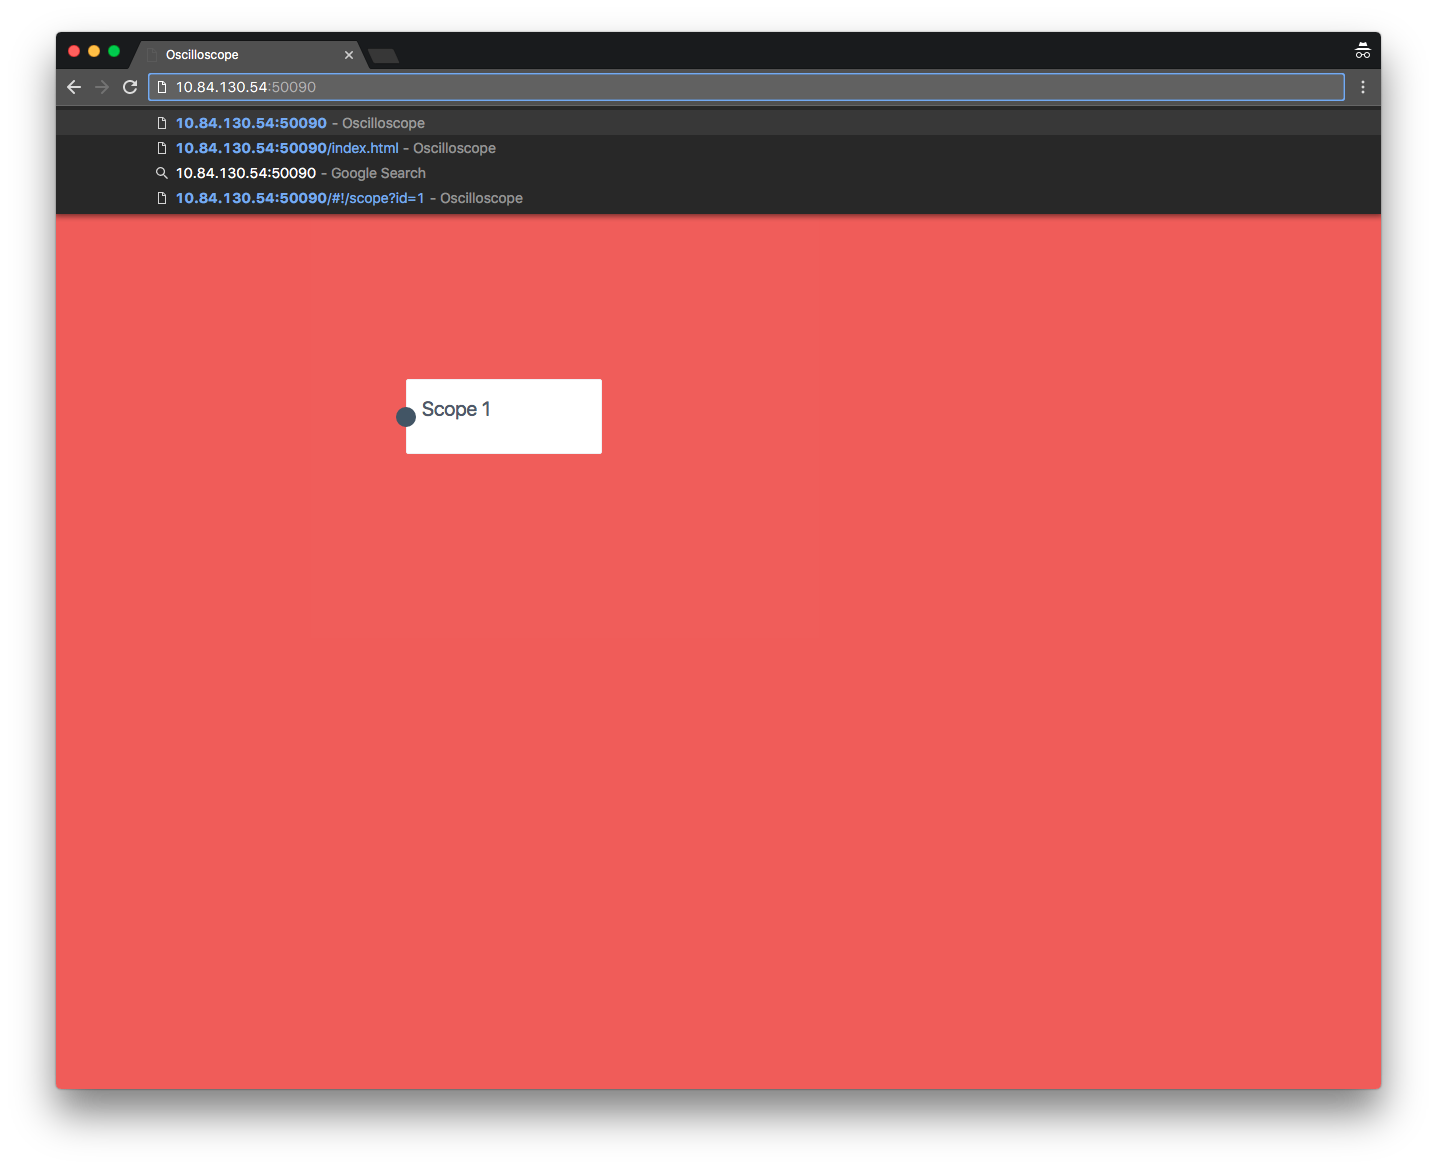
\includegraphics[width=0.75\textwidth]{images/userguide/url}
    \caption[Entering the URL]{%
        Using a browser and the correct URL to run the scope application on
        the STEMlab.
    }
    \label{fig:userguide:url}
\end{figure}

\begin{figure}
    \centering
    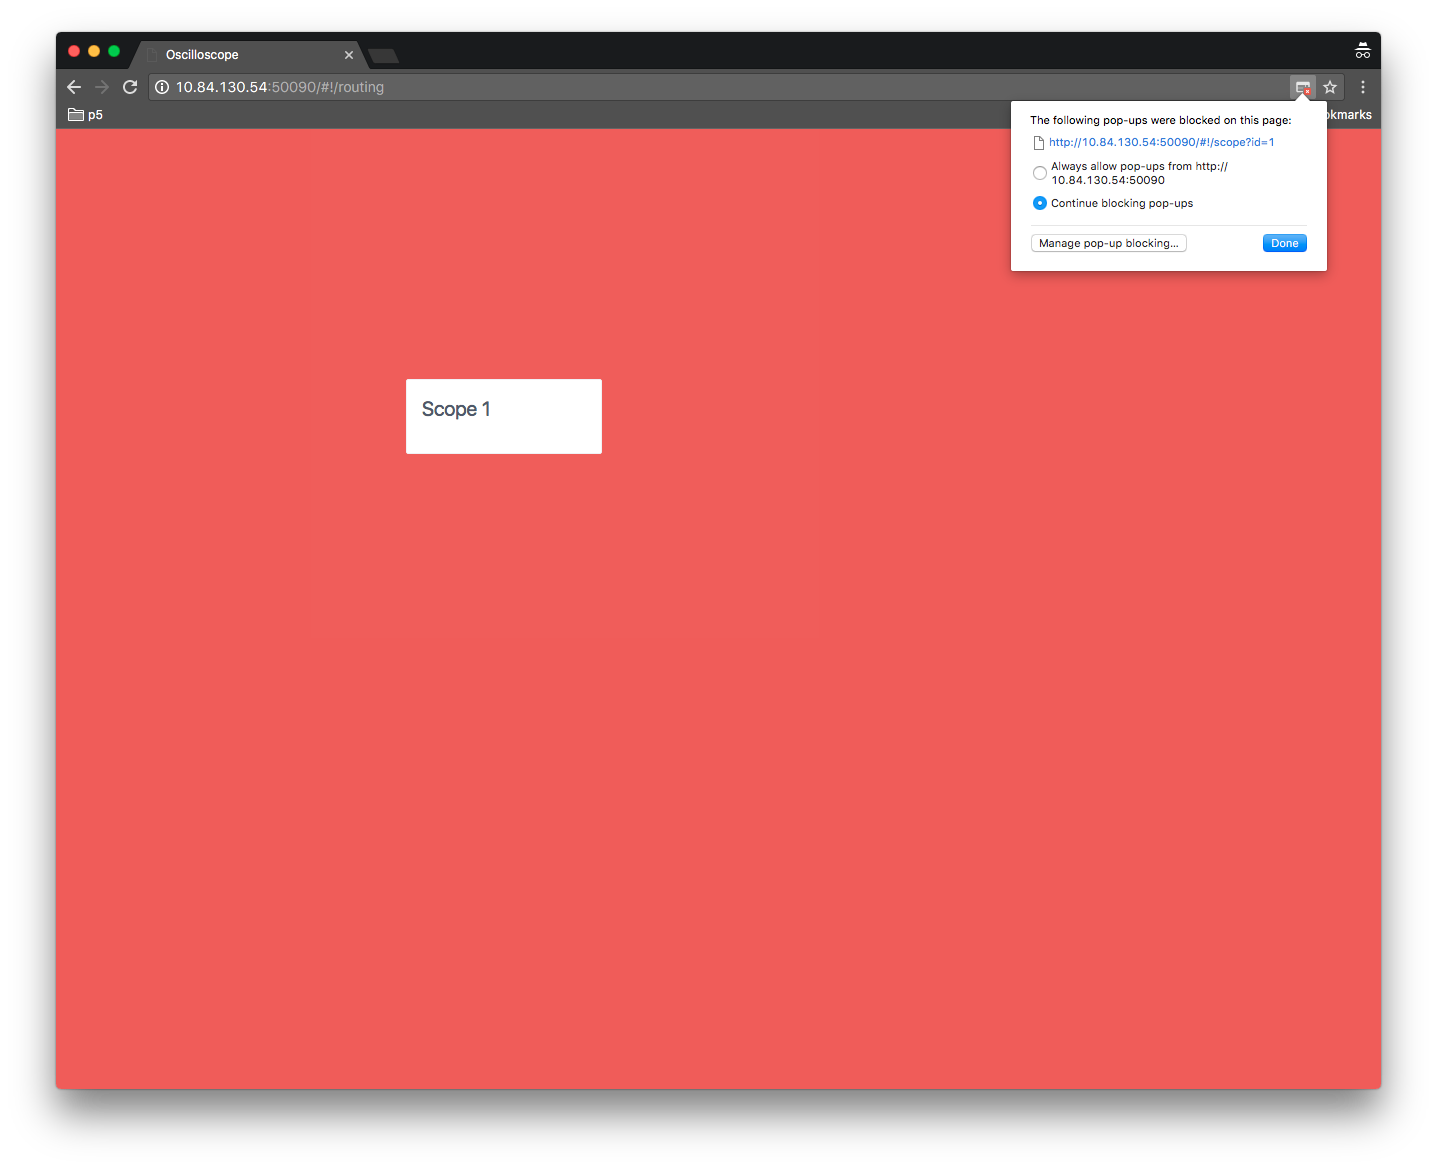
\includegraphics[width=0.75\textwidth]{images/userguide/popup_warn}
    \caption[The popup warn popup]{%
        The browser warns about a popup the site has tried to open.
    }
    \label{fig:userguide:popup:warn}
\end{figure}

\begin{figure}
    \centering
    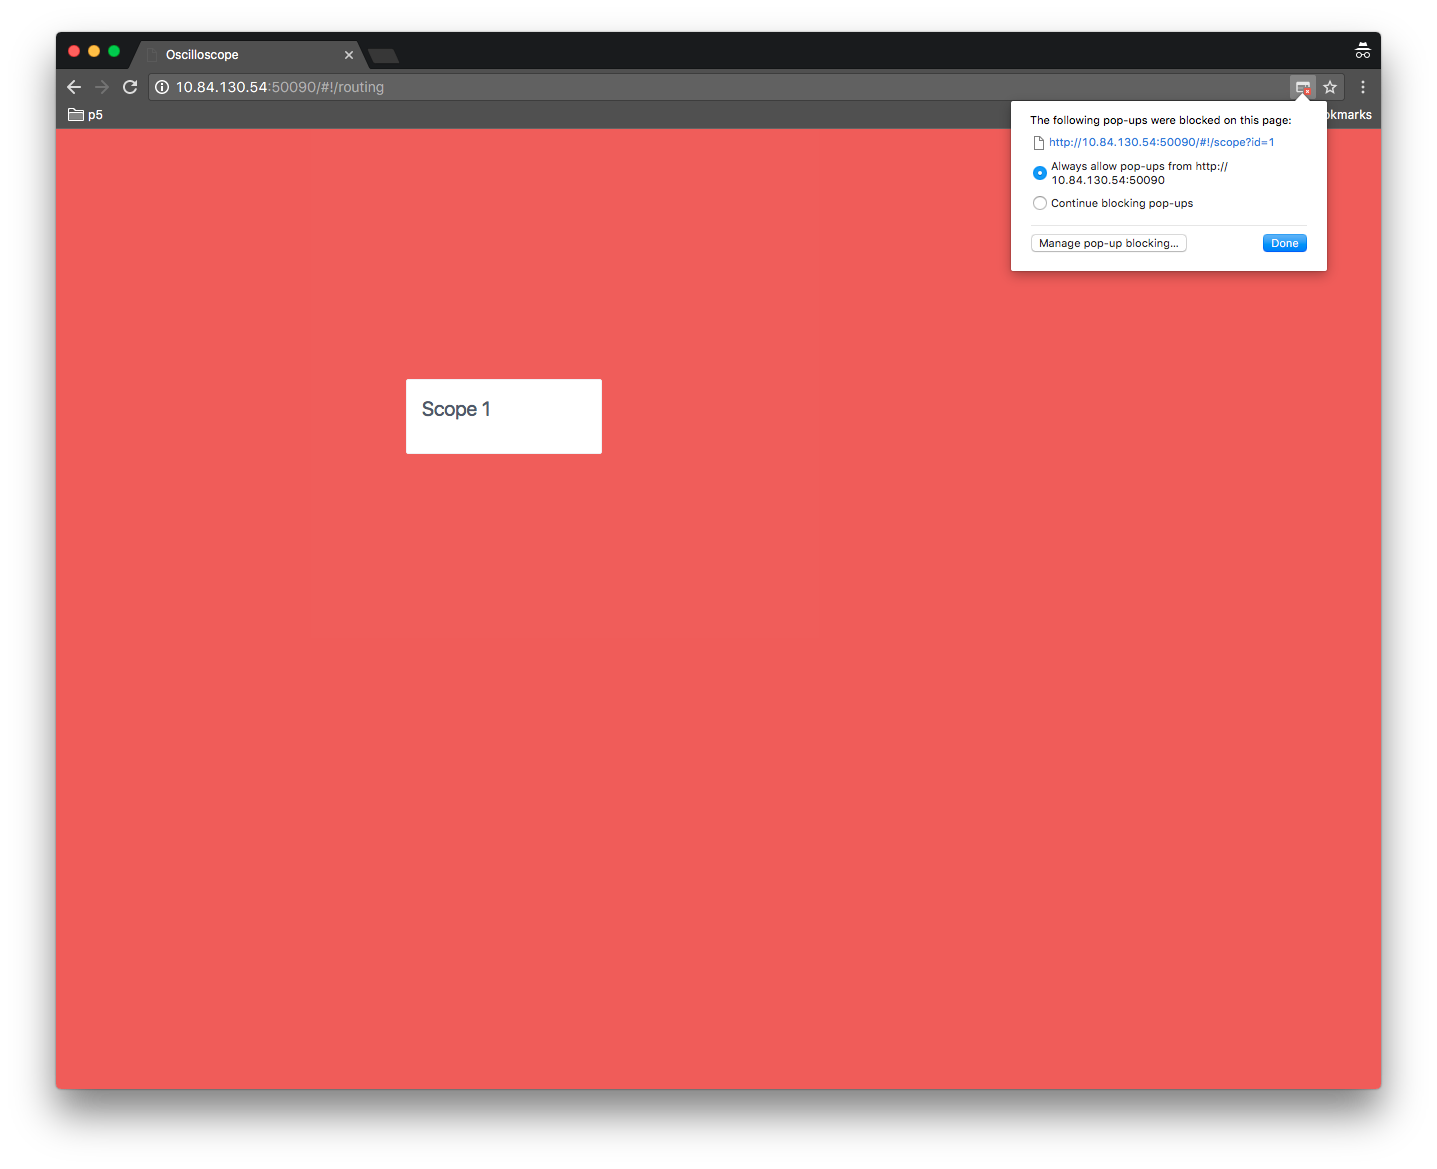
\includegraphics[width=0.75\textwidth]{images/userguide/popup_yes}
    \caption[Accept popups in the future]{%
        Let the browser accept popups in the future.
    }
    \label{fig:userguide:popup:yes}
\end{figure}

\begin{figure}
    \centering
    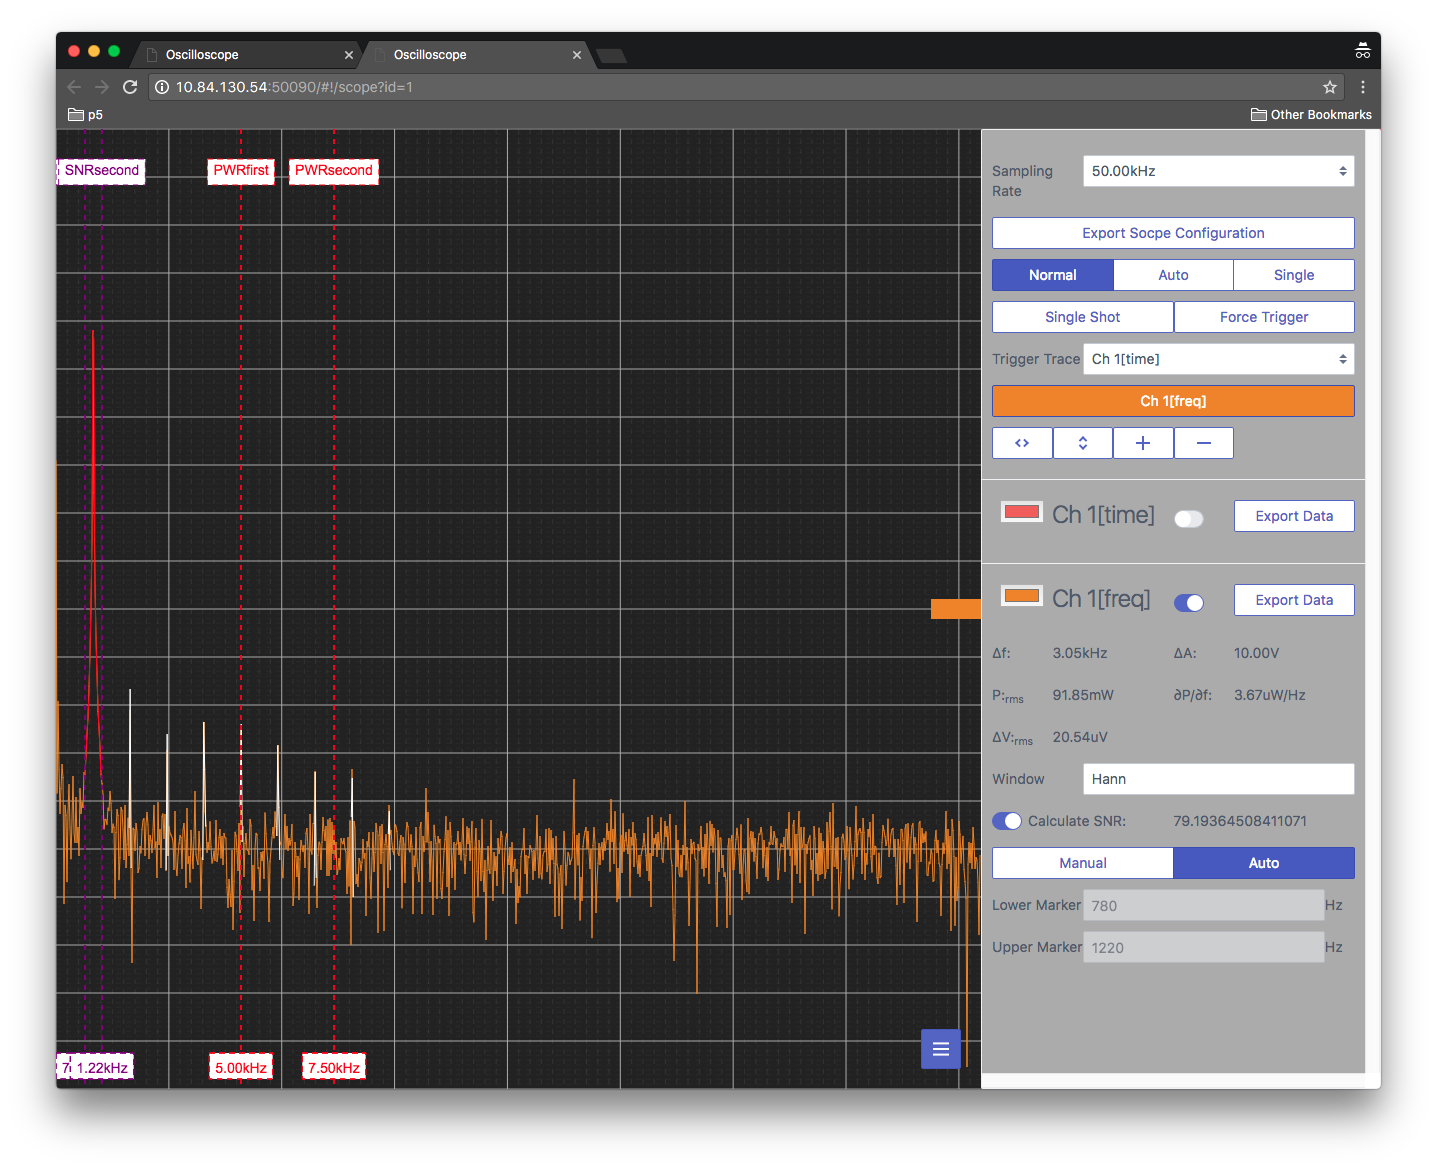
\includegraphics[width=0.75\textwidth]{images/userguide/running}
    \caption[Running the scope]{%
        The running scope after everything has been set up properly.
    }
    \label{fig:userguide:running}
\end{figure}

%>>>
% ==============================================================================
%
%                              O P E R A T I O N
%
% ==============================================================================
\chapter{Operation} % <<< ---------------------------------------------------- %
\label{ch:userguide:operation}
% ---------------------------------------------------------------------------- %

Once the oscilloscope  is running, interaction is done via  its graphical user
interface. Its  most important  features  are summarized  here.   It has  been
designed with high discoverability of its functionality in mind, so a complete
guide on every single  last button and menu is considered  beyond the scope of
this document.

Figure~\ref{fig:userguide:screenshot}  shows a  screenshot  of the  interface.
The UI's most important functions are:
\begin{description}
    \item[Zooming and Panning:]
        To zoom,  use the  vertical and horizontal  scrolling function  of the
        mouse or  trackpad.  To  pan, click  and drag  the signal. If  you are
        dragging a time trace it will automatically move the trigger location.

        The two arrow buttons in the general preference pane resize the signal
        to the visible area.
    \item[Triggering:]
        To set the trigger level, move the drawn trigger level by clicking and
        dragging it  or enter the level  in numbers on the  preference pane of
        the triggering time trace.
    \item[Markers:]
        There are four  markers by default. Two mark the start  and end of the
        area  over which  power  is  integrated and  two  mark  the area  that
        contains the signal for the automatic SNR calculation.

        Markers can be dragged and  moved by clicking and dragging. The number
        at the bottom of each marker shows the frequency it is at.

        The plus button in  the general pref pane adds a  new marker which can
        be used to mark certain frequencies.

        To move the SNR  markers, the SNR mode has to  be set from \emph{auto}
        to \emph{manual} mode in the corresponding FFT trace preference pane.
    \item[Sampling Rate:]
        To configure the  sampling rate, use the drop-down menu  at the top of
        the general preference pane.
    \item[Line Width:]
        To  improve  readability,  some  people  might  like  a  thicker  line
        width. To set the line width, use the  input at the top of the general
        pref pane.
\end{description}

\begin{figure}
    \centering
    \includegraphics[width=1\textwidth]{images/gui/scope}
    \caption[The Scope Application]{%
        The scope application in its current state, displaying time and FFT data%
    }
    \label{fig:usegruide:screenshot}
\end{figure}

%>>>

%^^A vim: foldenable foldcolumn=4 foldmethod=marker foldmarker=<<<,>>>

% >>>
% ==============================================================================
%
%                             A P P E N D I C E S
%
% ==============================================================================
\cleardoublepage % <<< ---------------------------------------------APPENDICES %
%                                                                        SETUP %
\begin{titlingpage*}
    \fullhexpage{da2}{ct4}
    \begin{vplace}
        \flushright\Huge\bfseries\sffamily\appendixpagename
    \end{vplace}
    \addcontentsline{toc}{part}{\partnumberline{Appendices}}{}
\end{titlingpage*}
\appendix
\chapterstyle{alpenappendix}
% ---------------------------------------------------------------------------- %
%                                                                       CHUNKS %
% ==============================================================================
%
%                 T H E O R E T I C A L   B A C K G R O U N D
%
% ==============================================================================
\chapter{Theoretical Background} % ------------------------------------------- %
\label{ch:app:theoretical_background}
% ---------------------------------------------------------------------------- %

This  chapter  contains  some  supplementary information  on  the  theoretical
background behind  this project. For those  who wish to better  understand the
internal  workings of  a CIC  filter, the first section  details exactly  what
happens inside a CIC filter for a very simple example. Simulink files are also
provided for further  study. The second section contains  tabulated values for
CIC filter design taken from~\cite{1163535}

\section{Internal Behavior of a CIC Filter} % <<< ---------------------------- %
\label{sec:app:cic_simu}
% ---------------------------------------------------------------------------- %

This  section presents  an example  for  a very  simple CIC  filter to  better
understand  its  internal  workings. For  verification,  the  filter  is  also
implemented in a Simulink model and simulated.

In the interest of simplicity, we choose  a filter with a decimation rate $R =
2$, a differential delay $M=1$ and $N=1$ stages. The corresponding topology is
shown in Figure~\ref{fig:cic_simu:topo}; Figure~\ref{fig:cic_simu:freqz} shows
the magnitude frequency  response of the filter. As can be  clearly seen, this
filter would be of very limited  use in practice. However, for the purposes of
this example, we  feed a DC  signal (a constant) into the  filter, so the
only thing  of importance is  the filter's DC  gain (which is  \SI{6}{\dB}, or
\num{2}).

Lastly,   we   restrict   numerical   accuracy  to   three   bits   in   two's
complement;  the  entire  range  of  representable  values  can  be  found  in
Figure~\ref{fig:cic_simu:twos_complement_circle}. This  limits  the number  of
steps  which need  to  be calculated  to  gain the  desired  insight into  the
filter's mathematical mechanics.

\begin{figure}
    \centering
    % https://tex.stackexchange.com/a/183092/131649
\tikzsetnextfilename{cicTopology}
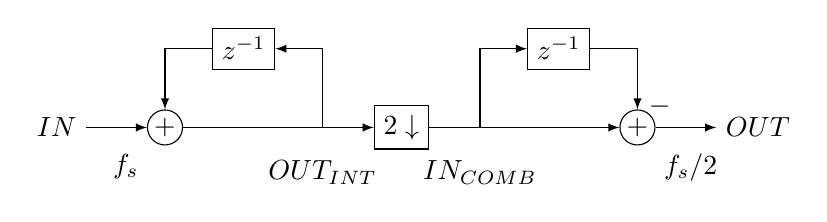
\begin{tikzpicture}
    \coordinate (in)  at (0,0);
    \coordinate (out) at (8,0);

    % branching coordinates
    \coordinate (b1) at (3,0);
    \coordinate (b2) at (5,0);

    % Delay elements
    \node[draw] (d1) at  (2,1) {$z^{-1}$};
    \node[draw] (d2) at  (6,1) {$z^{-1}$};

    % Downsampler
    \node[draw] (r1) at (4,0) {$2\downarrow$};

    % Adders
    \node[draw,circle, inner sep=0.3mm] (a1) at  (1,0) {$+$};
    \node[draw,circle, inner sep=0.3mm] (a2) at  (7,0) {$+$};

    % subtractors
    \node[above right=0.2ex] (s1) at (a2) {$-$};

    % Lines
    \draw[-latex] (in) -- (a1);
    \draw[-latex] (a1) -- (r1);
    \draw[-latex] (r1) -- (a2);
    \draw[-latex] (a2) -- (out);
    \draw[-latex] (b1) |- (d1);
    \draw[-latex] (b2) |- (d2);
    \draw[-latex] (d1) -| (a1);
    \draw[-latex] (d2) -| (a2);

    % Annotations
    \node[below left =2ex] at (a1) {$f_s$};
    \node[below right=2ex] at (a2) {$f_s/2$};
    \node[anchor=east] at (in) {$IN$};
    \node[anchor=west] at (out) {$OUT$};
    \node[anchor=north,below=2ex] at (b1) {$OUT_{INT}$};
    \node[anchor=north,below=2ex] at (b2) {$IN_{COMB}$};
\end{tikzpicture}

    \caption[Topology of Example Filter]{Topology of the CIC filter for this example}
    \label{fig:cic_simu:topo}
\end{figure}

\begin{figure}
    \centering
    \newcommand*\freqzFileInt{images/cicSimu/cic1.csv}
\pgfplotstableread[col sep=comma]{\freqzFileInt}\freqzTableInt
\begin{tikzpicture}[
        spy using outlines={magnification=4, connect spies}
    ]
     \pgfplotsset{every axis/.style={
            height=60mm,
            width=\textwidth,
            grid=none,
            y filter/.code={\pgfmathparse{20*log10(\pgfmathresult))}},
            x filter/.code={\pgfmathparse{\pgfmathresult / 3.141592654}},
            xticklabel style={font=\footnotesize},
            x unit=\times\,\pi\,\si{\radian}/\si{\sample},
            y unit=\si{dB},
            xlabel=Normalized Frequency,
            ylabel=Magnitude,
        },
        every axis legend/.append style={
            at={(1,-0.25)},  % if attached to bottom plot
            anchor=north east,
            cells={anchor=east},
        },
    }
    \begin{axis}[
            title=Integrator Frequency Responses,
            at = {(0,0)},
            xmin=0,
            xmax=1,
            xtick={0,0.5,1},
            ytick={6,0,-20,-40},
            xticklabels={0,$f_s/4$,$f_s/2$},
        ]
        \addplot[thick,q1,-] table[x=w, y=abs(H)] \freqzTableInt;
    \end{axis}
\end{tikzpicture}

    \caption[Frequency Respose of Example CIC Filter]{%
        Frequency response of a CIC  filter with $N=1$, $M=1$, $R=2$. Note the
        DC gain of \num{2}.%
    }
    \label{fig:cic_simu:freqz}
\end{figure}

The  state  of  the  filter  can  be  calculated  by  the  formulas  given  in
Equations~\ref{eq:cic_simu:INT} and \ref{eq:cic_simu:OUT}:
\begin{align}
    N             & = 1 \quad M = 1 \quad R=2\nonumber\\
    OUT_\mathrm{INT}[n]  & = IN_\mathrm{COMB}[n] = IN[n]        + OUT[n-1]
    \label{eq:cic_simu:INT} \\
    OUT_\mathrm{COMB}[n] & = IN_\mathrm{COMB}[n] - IN_\mathrm{COMB}[n-R\cdot M]
    \nonumber\\
                  & = OUT_\mathrm{INT}[n] - OUT_\mathrm{INT}[n-2]
    \label{eq:cic_simu:OUT}
\end{align}

The  input  of the  filter  shall  be a  constant  of  $1$, starting  at  time
zero. Once this  input is  applied to  the system,  the integrator  stage will
begin  to  accumulate  the  constant. Given  an  unlimited  number  of  digits
(bits),  the integrator  would in  theory reach  infinity if  it kept  running
forever. In practice, however, it wraps around once it has reached its maximum
representable value  (\code{011}~$ =  3$) and begins  counting from  its lower
numerical limit  (\code{100}~$=-4$) again. This cycle keeps  repeating as long
as the filter is running.

The  ingenuity of  the  CIC filter  lies  in exploiting  the  fact that  this
wraparound is irrelevant to the  comb stage. Whether the comb stage calculates
the difference between  an integrator's value whose precision  is unbounded or
whether it calculates the difference between two values which have potentially
been  wrapped  is  without  consequence.

As a  demonstration of this effect,  we shall examine the  computation step of
cycle $n = 4$  from Table~\ref{tab:cic_simu:cic_filter_states} (which contains
the  entire filter's  state for  15 steps). At  this point,  the state  of the
filter's output is  as follows (represented in three-bit  two's complement and
decimal):
\begin{align}
    OUT_\mathrm{COMB}[4]_\mathrm{b} &= OUT_{INT}[4] - OUT_{INT}[2]     \nonumber\\
                             &= 101_\mathrm{b} - 011_\mathrm{b} \nonumber\\
                             &= 010_\mathrm{b}
    \label{eq:cic_simu:stage4:binary} \\
    OUT_\mathrm{COMB}[4]_\mathrm{d} &= -3_\mathrm{d} - 3_\mathrm{d}    \nonumber\\
                             &= -6_\mathrm{d}
    \label{eq:cic_simu:stage4:decimal:bounded}
\end{align}
Obviously,   the  decimal   and   binary  results   do   not  match. This   is
where   the  wraparound   comes   into   play,  for   which   we  shall   look
at  Figure~\ref{fig:cic_simu:twos_complement_circle}. The  figure  presents  a
circular  arrangement  for   all  numbers  in  two's   complement  with  three
digits  precision.   In  that  arrangement,  addition  of  a  positive  number
corresponds to  moving clockwise  through the circle,  while subtraction  of a
positive number means moving  counterclockwise. Doing this for the calculation
of  Equation~\ref{eq:cic_simu:stage4:decimal:bounded},  we  find  that  moving
by  three  in  the  counterclockwise   direction  lands  us  at  $2$,  exactly
as   Equation~\ref{eq:cic_simu:stage4:binary}  demands. The   computation  has
\emph{wrapped around} its boundary ($-4$).

What     is     left    to     verify     is     that    the     result     of
Equation~\ref{eq:cic_simu:stage4:binary} is indeed the correct result, i.e. if
an  unbounded integrator  and comb  would have  yielded the  same outcome. And
indeed, they would have:
\begin{equation}
    \label{eq:cic_simu:stage4:decimal:unbounded}
    OUT_\mathrm{COMB}[6] = 7 - 5 = 2
\end{equation}

\begin{figure}
    \centering
    \tikzsetnextfilename{twosComplementCircle}
\begin{tikzpicture}
    \node (b1) at   (0:2.5) {\texttt{010}};
    \node (b2) at  (45:2.5) {\texttt{001}};
    \node (b3) at  (90:2.5) {\texttt{000}};
    \node (b4) at (135:2.5) {\texttt{111}};
    \node (b5) at (180:2.5) {\texttt{110}};
    \node (b6) at (225:2.5) {\texttt{101}};
    \node (b7) at (270:2.5) {\texttt{100}};
    \node (b8) at (315:2.5) {\texttt{011}};

    \node (d1) at   (0:3.5) {\footnotesize$2$};
    \node (d2) at  (45:3.5) {\footnotesize$1$};
    \node (d3) at  (90:3.5) {\footnotesize$0$};
    \node (d4) at (135:3.5) {\footnotesize$-1$};
    \node (d5) at (180:3.5) {\footnotesize$-2$};
    \node (d6) at (225:3.5) {\footnotesize$-3$};
    \node (d7) at (270:3.5) {\footnotesize$-4$};
    \node (d8) at (315:3.5) {\footnotesize$3$};

    \draw[thick,q5,-latex]
        (b6)
        edge[out=315,in=180]
        node[midway,anchor=north east] {\texttt{-1}}
        (b7);
    \draw[thick,q5,-latex]
        (b7)
        edge[out=  0,in=225]
        node[midway,anchor=north] {\texttt{-1}}
        (b8);
    \draw[thick,q5,-latex]
        (b8)
        edge[out= 45,in=270]
        node[midway,anchor=north west] {\texttt{-1}}
        (b1);

    \draw[thick,q5,-latex] (0:1.5) arc[start angle= 0, end angle= 240, radius=1.5cm];
    \draw[thick,q1,-latex] (60:1.0) arc[start angle=60, end angle=-180, radius=1.0cm];

    \node at (120:1.25) {\color{q5}$-$};
    \node at (-60:0.75) {\color{q1}$+$};
\end{tikzpicture}

    \caption[Two's Complement Circle]{%
        Subtracting  $3$  from $-3$  in  two's  complement with  three  digits
        precision,  represented on  a  circle. Addition of  a positive  number
        corresponds  to moving  clockwise,  subtraction of  a positive  number
        corresponds to moving counterclockwise.%
    }
    \label{fig:cic_simu:twos_complement_circle}
\end{figure}

\begin{table}
    \centering
    \caption[CIC Filter Example: States for 16 Cycles]{%
        Binary and  decimal values  for the  different filter  elements during
        various  stages  of the  filtering  process. As  expected due  to  the
        filter's  DC gain  of \num{2},  its output  is \num{2}. The  two right
        columns contain the  calculations as they would occur  if the filter's
        components had unbounded precision. It can be seen that the wraparound
        effect of the  two's complement representation does  indeed not change
        the filter's output.%
    }
    \label{tab:cic_simu:cic_filter_states}
    \ttfamily
    \begin{tabular}{rrrr|rrr}
        \toprule
        \scshape Cycle                   &
        \scshape IN                      &
        \scshape OUT\textsubscript{INT}  &
        \scshape OUT                     &
        \scshape OUT\textsubscript{INT}  &
        \scshape OUT                     &
        \scshape OUT                     \\

        &
        &
        \scshape IN\textsubscript{COMB} &
        &
        (unbounded) &
        (bounded    &
        (unbounded  \\

        &
        &
        &
        &
        &
        integrator) &
        integrator) \\

        \midrule
        %     IN   OI/IC  OUT   UW
        -2 & 000 &  000 & 000 & $ 0$ &                                    & \\
        -1 & 000 &  000 & 000 & $ 0$ &                                    & \\
         0 & 001 &  001 & 001 & $ 1$ & $  1 -   0  =  1                 $ & $ 1 - 0 = 1 $\\
         1 & 001 &  010 &     & $ 2$ &                                    & \\
         2 & 001 &  011 & 010 & $ 3$ & $  3 -   1  =  2                 $ & $ 3 - 1 = 2 $\\
         3 & 001 &  100 &     & $ 4$ &                                    & \\
         4 & 001 &  101 & 010 & $ 5$ & $ -3 -   3  = -6 = 2_\mathrm{wr} $ & $ 5 - 3 = 2 $\\
         5 & 001 &  110 &     & $ 6$ &                                    & \\
         6 & 001 &  111 & 010 & $ 7$ & $ -1 - (-3) =  2                 $ & $ 7 - 5 = 2 $\\
         7 & 001 &  000 &     & $ 8$ &                                    & \\
         8 & 001 &  001 & 010 & $ 9$ & $  1 - (-1) =  2                 $ & $ 9 - 7 = 2 $\\
         9 & 001 &  010 &     & $10$ &                                    & \\
        10 & 001 &  011 & 010 & $11$ & $  3 -   1  =  2                 $ & $ 11 - 9 = 2 $\\
        11 & 001 &  100 &     & $12$ &                                    & \\
        12 & 001 &  101 & 010 & $13$ & $ -3 -   3  = -6 = 2_\mathrm{wr} $ & $ 13 - 11 = 2 $\\
        13 & 001 &  110 &     & $14$ &                                    & \\
        14 & 001 &  111 & 010 & $15$ & $ -1 - (-3) =  2                 $ & $ 15 - 13 = 2 $\\
        \bottomrule
    \end{tabular}
\end{table}

As  a   last  step   to  confirm   our  results,  the   CIC  filter   of  this
exercise  is   simulated  with   Simulink. Its  block   design  is   given  in
Figure~\ref{fig:cic_simu:simulink_model}. All   blocks   are  set   to   two's
complement with three digits of precision (no fractional bits).

The          simulation         results          are         given          in
Figure~\ref{fig:cic_simu:simulink_results}. As   can  be   seen,  the   filter
states  are  identical  to  our manually  calculated  example. The  effect  of
the  integrator's   output  wrapping   around  the  numerical   boundaries  is
also  nicely  visible. In  case  the  reader  wishes  to  tinker  around  with
this  themselves,  the  Simulink  files  can  be  found  in  the  subdirectory
\code{doc/report/images/cicSimu}, relative  to the repository  root. Note that
the fixed-point toolbox is required for this.

\begin{figure}
    \centering
    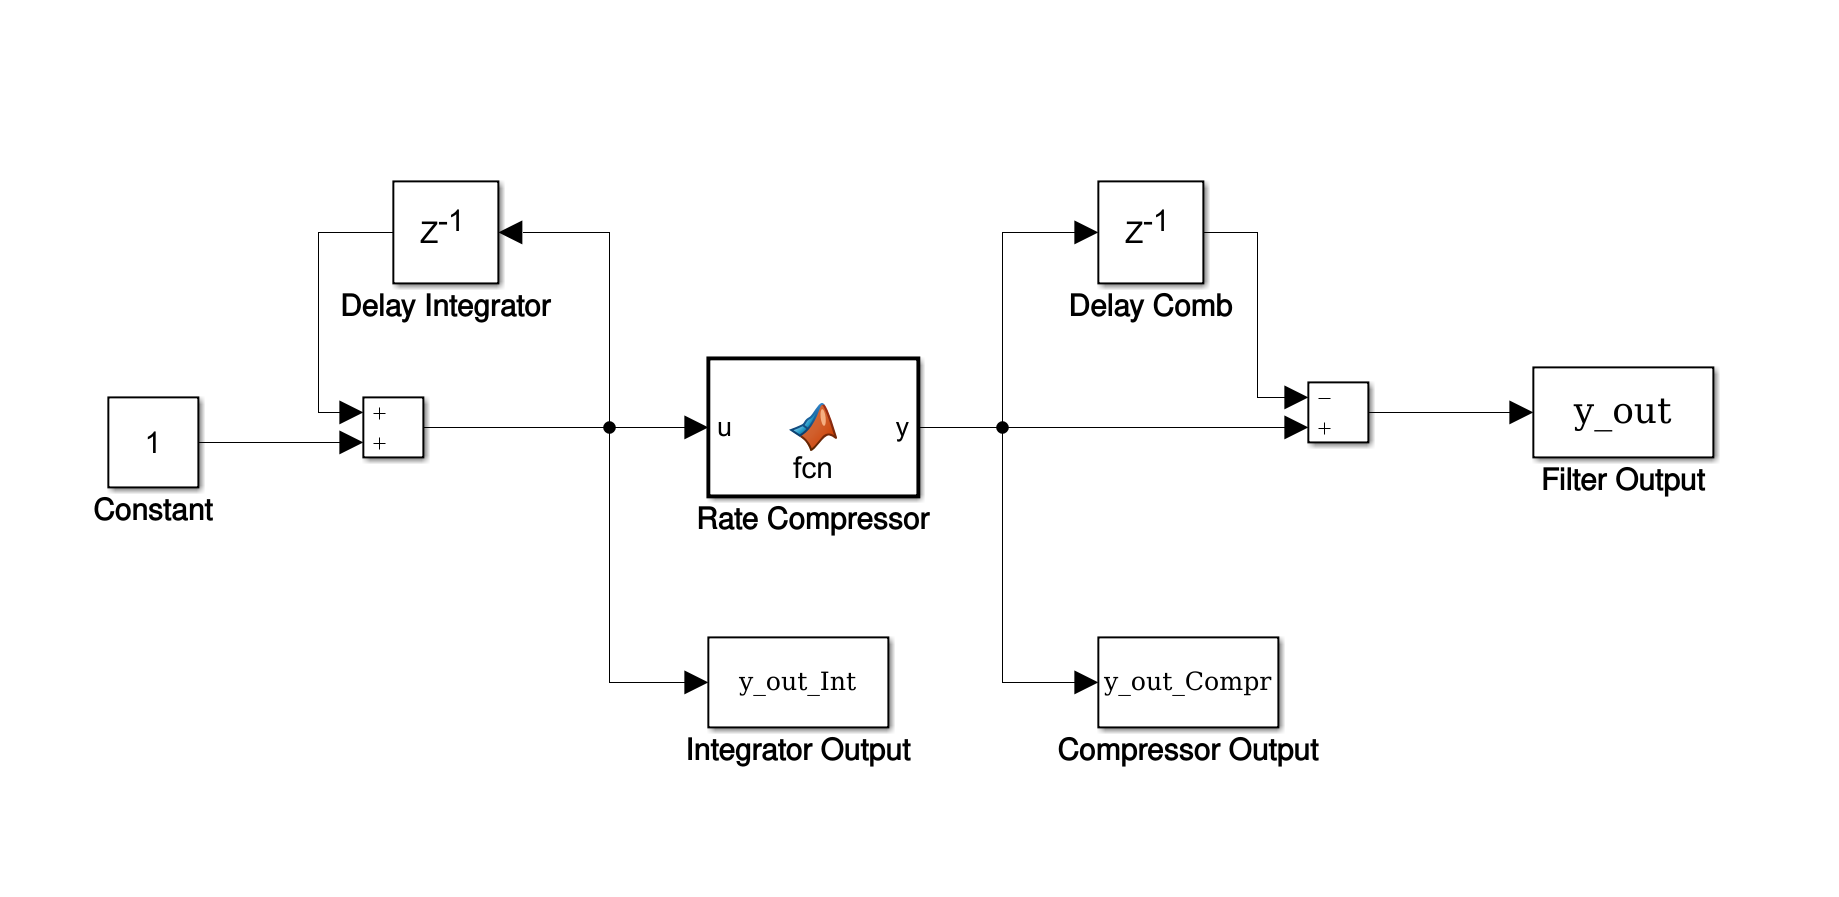
\includegraphics[width=\textwidth]{images/cicSimu/simulink.png}
    \caption[Simulink Filter Model]{%
        Simulink model  for the filter  in Figure~\ref{fig:cic_simu:topo}. The
        Rate   Compressor is  a  simple Matlab  function  which returns  every
        second value of its input vector.%
    }
    \label{fig:cic_simu:simulink_model}
\end{figure}

\begin{figure}
    \centering
    \newcommand*\freqzFileIntA{images/cicSimu/simulinkYout.csv}
\newcommand*\freqzFileIntB{images/cicSimu/simulinkYoutCompr.csv}
\newcommand*\freqzFileIntC{images/cicSimu/simulinkYoutInt.csv}
\pgfplotstableread[col sep=comma]{\freqzFileIntA}\freqzTableIntA
\pgfplotstableread[col sep=comma]{\freqzFileIntB}\freqzTableIntB
\pgfplotstableread[col sep=comma]{\freqzFileIntC}\freqzTableIntC
\begin{tikzpicture}
    \pgfplotsset{every axis/.style={
            height=50mm,
            width=\textwidth,
            grid=none,
            xmin=-1,
            xmax=15,
            xtick={0,2,4,6,8,10,12,14},
            ytick={-4,-2,0,2,4},
            ylabel=$OUT$,
            xlabel=$n$,
        },
    }
    \begin{axis}[
            title=Filter Output,
            at = {(0,0)},
            ytick={0,1,2},
            ymin=0,
        ]
        \addplot[ycomb,mark=*,dv+5,-] table[x=t,y=y] \freqzTableIntA;
    \end{axis}

    \begin{axis}[
            title=Compressor Output (Comb Input),
            at = {(0,-55mm)},
            ymin=-4,
            ymax=4,
        ]
        \addplot[ycomb,mark=*,dv+5,-] table[x=t,y=y] \freqzTableIntB;
        \draw[gray] (rel axis cs:0,0.5) -- (rel axis cs:1,0.5);
    \end{axis}

    \begin{axis}[
            title=Integrator Output,
            at = {(0,-110mm)},
            ymin=-5,
            ymax=4,
        ]
        \addplot[ycomb,mark=*,dv+5,-] table[x=t,y=y] \freqzTableIntC;
        \draw[gray] (-1,0) -- (15,0);
    \end{axis}
\end{tikzpicture}

    \caption[Simulink Simulation Results]{%
        Simulation    results    from    Simulink   for    the    filter    in
        Figure~\ref{fig:cic_simu:simulink_model}%
    }
    \label{fig:cic_simu:simulink_results}
\end{figure}

Lastly,  it is  shown what  happens  when the  expected output  of the  filter
exceeds  the numerical  range  available. This is  accomplished  by feeding  a
constant of \num{2} into the filter; the expected output is therefore \num{4}.

Because \num{4}  is not  within the  range of  a three-digit  two's complement
number  system, the  filter wraps  around  and produces  an incorrect  output,
\num{-4}.   The  first  few  calculation  steps  for  this  are  presented  in
Table~\ref{tab:cic_simu:cic_filter_states:out_of_bounds};  running  the  above
simulation with the modified input also confirms this result.

\begin{table}
    \centering
    \caption[CIC Filter Example: Output Out of Range]{%
        The  same CIC  filter  as  before stimulated  with  an  input of  2. A
        comparison between the right two columns  shows that the output of the
        bounded filter and its unbounded  counterpart no longer match starting
        with the output at $n=2$; the filter produces a false output.%
    }
    \label{tab:cic_simu:cic_filter_states:out_of_bounds}
    \ttfamily
    \begin{tabular}{rrrr|rrr}
        \toprule
        \scshape Cycle                   &
        \scshape IN                      &
        \scshape OUT\textsubscript{INT}  &
        \scshape OUT                     &
        \scshape OUT\textsubscript{INT}  &
        \scshape OUT                     &
        \scshape OUT                     \\

        &
        &
        \scshape IN\textsubscript{COMB} &
        &
        (unbounded) &
        (bounded    &
        (unbounded  \\

        &
        &
        &
        &
        &
        integrator) &
        integrator) \\

        \midrule
        %     IN   OI/IC  OUT   UW
        -2 & 000 &  000 & 000 & $ 0$ &                        & \\
        -1 & 000 &  000 & 000 & $ 0$ &                        & \\
         0 & 010 &  010 & 010 & $ 2$ & $  2 -   0  =  2     $ & $ 2 - 0 = 2 $\\
         1 & 010 &  100 &     & $ 4$ &                        & \\
         2 & 010 &  110 & 100 & $ 6$ & $ -2 -   2  = -4     $ & $ 6 - 2 = 4 $\\
         3 & 010 &  000 &     & $ 8$ &                        & \\
         4 & 010 &  010 & 100 & $10$ & $  2 - (-2) = -4     $ & $10 - 6 = 4 $\\
        \bottomrule
    \end{tabular}
\end{table}
%>>>
\clearpage
\section{CIC Filter Tables} % <<< -------------------------------------------- %
\label{sec:app:cic_filter_tables}
% ---------------------------------------------------------------------------- %

\begin{table}[h]
    \centering
    \caption[CIC Filter Passband Attenuations]{%
        Passband  attenuation   for  CIC   filters  as   a  function   of  the
        bandwidth-differential delay product. Taken from~\cite{1163535}.%
    }
    \label{tab:cic:pb_attenuation}
    \begin{tabular}{rrrrrrrr}
        \toprule
            \parbox[t]{40mm}{
                Relative \\
                Bandwidth-Differential\\
                Delay Product ($Mf_c$)} &
            \multicolumn{7}{c}{\parbox[t]{60mm}{
                Passband attenuation at $f_c$ in \si{\dB} \\
                as a Function of \\
                Number of Stages ($N$)}}                                  \\
        \midrule
            & 1 & 2 & 3 & 4 & 5 & 6 \\
        \midrule
            $1/128$ & $0.00$ & $0.00$ & $0.00$ & $0.00$ & $0.00$ & $0.01$ \\
            $1/64 $ & $0.00$ & $0.01$ & $0.01$ & $0.01$ & $0.02$ & $0.02$ \\
            $1/32 $ & $0.01$ & $0.03$ & $0.04$ & $0.06$ & $0.07$ & $0.08$ \\
            $1/16 $ & $0.06$ & $0.11$ & $0.17$ & $0.22$ & $0.28$ & $0.34$ \\
            $1/8  $ & $0.22$ & $0.45$ & $0.67$ & $0.90$ & $1.12$ & $1.35$ \\
            $1/4  $ & $0.91$ & $1.82$ & $2.74$ & $3.65$ & $4.56$ & $5.47$ \\
        \bottomrule
    \end{tabular}
\end{table}

\begin{table}[h]
    \centering
    \caption[CIC Filter Passband Aliasing Attenuation]{%
        Passband aliasing  attenuation for  CIC filters as  a function  of the
        bandwidth and the differential delay. Taken from~\cite{1163535}.%
    }
    \label{tab:cic:pb_aliasing}
    \begin{tabular}{rrrrrrrrr}
        \toprule
            \parbox[t]{20mm}{
                Differential\\
                Delay\\
                ($M$)%
            } &
            \parbox[t]{20mm}{
                Relative \\
                Bandwidth\\
                ($f_c$)} &
            \multicolumn{7}{c}{\parbox[t]{70mm}{
                Aliasing/Imaging Attenuation at $f_\mathrm{s,low}$ in \si{\dB}\\
                as a Function of Number of Stages ($N$)}}\\
        \midrule
            & & 1 & 2 & 3 & 4 & 5 & 6 \\
        \midrule
            1 & $1/128$ & $42.1$ & $84.2$ & $126.2$ & $168.3$ & $210.4$ & $252.5$ \\
            1 & $1/64 $ & $36.0$ & $72.0$ & $108.0$ & $144.0$ & $180.0$ & $215.9$ \\
            1 & $1/32 $ & $29.8$ & $59.7$ & $ 89.5$ & $119.4$ & $149.2$ & $179.0$ \\
            1 & $1/16 $ & $23.6$ & $47.2$ & $ 70.7$ & $ 94.3$ & $117.9$ & $141.5$ \\
            1 & $1/8  $ & $17.1$ & $34.3$ & $ 51.4$ & $ 68.5$ & $ 85.6$ & $102.8$ \\
            1 & $1/4  $ & $10.5$ & $20.9$ & $ 31.4$ & $ 41.8$ & $ 52.3$ & $ 62.7$ \\
        \midrule
            2 & $1/256$ & $48.1$ & $96.3$ & $144.4$ & $192.5$ & $240.7$ & $288.8$ \\
            2 & $1/128$ & $42.1$ & $84.2$ & $126.2$ & $168.3$ & $210.4$ & $252.5$ \\
            2 & $1/64 $ & $36.0$ & $72.0$ & $108.0$ & $144.0$ & $180.0$ & $216.0$ \\
            2 & $1/32 $ & $29.9$ & $59.8$ & $ 89.6$ & $119.5$ & $149.4$ & $179.3$ \\
            2 & $1/16 $ & $23.7$ & $47.5$ & $ 71.2$ & $ 95.0$ & $118.7$ & $179.3$ \\
            2 & $1/8  $ & $17.8$ & $35.6$ & $ 53.4$ & $ 71.3$ & $ 89.1$ & $106.9$ \\
        \bottomrule
    \end{tabular}
\end{table}
%>>>

%^^A vim: foldenable foldcolumn=4 foldmethod=marker foldmarker=<<<,>>>

% ==============================================================================
%
%                          F I L T E R   D E S I G N
%
% ==============================================================================
\chapter{Filter Design} % ---------------------------------------------------- %
\label{ch:app:fdesign}
% ---------------------------------------------------------------------------- %

Some  additional information  about  the filter  design  process is  presented
here. This  comprises  a graphical  comparison  between  two variants  of  the
$R=625$  filter  chain,  measurements  for  resource  usage  on  the  FPGA  in
relation  to  filter  size,  and  the  frequency  responses  for  all  filters
and  filter  chains  as  designed  by Matlab  (for  measurement  results,  see
Chapter~\ref{ch:verification}). For studying  the filters  and chains  in more
detail, the reader is referred to the design files themselves.

% ==============================================================================
%
%                        D E C 6 2 5   V A R I A N T S
%
% ==============================================================================
\section{Decimation of 625: Variants} % <<< ---------------------------------- %
\label{sec:dec625_variants}
% ---------------------------------------------------------------------------- %

There are many possible  ways to implement a filter chain  for a given overall
downsampling  ratio $R$. Here,  two  possibilities are  compared for  $R=625$,
consisting  of  a  $125  \rightarrow  5$  cascade  and  a  $25  \rightarrow  5
\rightarrow 5$ cascade. In  both cascades, the initial stage is  a CIC filter,
followed by  a FIR compensator  and one or  more FIR filters. The  results are
shown in Figure~\ref{fig:dec625_variants}.

\begin{figure}
    \centering
    \tikzsetnextfilename{dec625VariantsFreqResponse}
\newcommand*\freqzFileDECA{images/fdesign/dec625--125-5.csv}
\newcommand*\freqzFileDECB{images/fdesign/dec625--25-5-5.csv}
\pgfplotstableread[col sep=comma]{\freqzFileDECA}\freqzTableDECA
\pgfplotstableread[col sep=comma]{\freqzFileDECB}\freqzTableDECB
\begin{tikzpicture}[
    trim axis left,
    trim axis right,
]
     \pgfplotsset{every axis/.style={
            height=45mm,
            width=\textwidth,
            grid=none,
            x unit=\times\,\pi\,\si{\radian}/\si{\sample},
            ylabel=Magnitude,
            xlabel=Normalized Frequency,
            xmin=0,
            xmax=3e-3,
            %xmin=0,
            %xmax=1000000,
            %ymax=5,
            %ymin=-120,
            legend columns=2,
            every axis legend/.append style={
                at={(0.5,-0.30)},  % if attached to bottom plot
                anchor=north,
                cells={anchor=west},
            },
        },
    }
    \begin{axis}[
            title={Decimation of $R=625$: Variants},
            at = {(0,0)},
            y unit=\si{dB},
            ymax=5,
            ymin=-180,
            y filter/.code={\pgfmathparse{20*log10(\pgfmathresult))}},
            x filter/.code={\pgfmathparse{\pgfmathresult / 3.141592654}},
        ]
        \addplot[thick,q1,-] table[x=W, y=abs(H)] \freqzTableDECA;
        \addplot[thick,q5,-] table[x=W, y=abs(H)] \freqzTableDECB;
    \end{axis}
    \begin{axis}[
            at = {(0,-62mm)},
            x filter/.code={\pgfmathparse{\pgfmathresult / 3.141592654}},
            %xtick={0,0.3e6,0.4e6,1e6},
        ]
        \addplot[thick,q1,-] table[x=W, y=abs(H)] \freqzTableDECA;
        \addplot[thick,q5,-] table[x=W, y=abs(H)] \freqzTableDECB;
    \end{axis}
    \begin{axis}[
            at = {(0,-124mm)},
            ylabel=Phase,
            y unit=\si{\degree},
            ymin=-2800,
            ymax=0,
            y filter/.code={\pgfmathparse{180*\pgfmathresult/3.141592654}},
            unbounded coords=discard,
            point meta=explicit,
            filter point/.code={%
                \pgfmathparse{\pgfkeysvalueof{/data point/meta}==0}
                \ifpgfmathfloatcomparison
                    \pgfkeyssetvalue{/data point/y}{nan}%
                \fi
            }
        ]
        \addplot[thick,-,q1,] table[x=W,y=angle(H),meta=abs(H)] \freqzTableDECA;
        \addplot[thick,-,q5] table[x=W,y=angle(H),meta=abs(H)] \freqzTableDECB;
        \legend{%
            $125 \rightarrow \text{CFIR} \rightarrow 5$,
            $ 25 \rightarrow \text{CFIR} \rightarrow 5 \rightarrow 5$%
        };
    \end{axis}
\end{tikzpicture}

    \caption[Decimation Chain Variants for Rate of 625]{%
        Semilog  (top)  and   linear  plot  (middle)  for   two  variants  for
        implementing  a  decimation   chain  for  a  rate   change  factor  of
        $R=625$. Both choices  show almost the  same behavior with  regards to
        magnitude. The  bottom  plot  shows  the phase  response  of  the  two
        filters; here, too, the behavior  is very similar. \emph{Note:}  These
        plots show  the frequency responses  of the entire filter  cascade for
        the two respective variants.%
    }
    \label{fig:dec625_variants}
\end{figure}

%>>>
\clearpage
% ==============================================================================
%
%                         R E S O U R C E   U S A G E
%
% ==============================================================================
\section{Resource Usage for FIR Filters on the FPGA} % <<< ------------------- %
\label{sec:fir_filter_resouce_usage}
% ---------------------------------------------------------------------------- %

Measurements   on    resource   usage    for   various   FIR    filters   have
been   performed    and   are    presented   here. The   objective    was   to
determine   how   many   DSP   slices   a  given   FIR   filter   needs   when
implemented   with  Xilinx's   FIR  Compiler~\cite{xilinx:fir-compiler}. These
figures   form   the    basis   to   define   reasonable    bounds   for   the
FIR   filter   \code{5steep}  (see   Figure~   \ref{fig:fdesign:chain_concept}
on    page~\pageref{fig:fdesign:chain_concept}). Figure~\ref{fig:usage_report}
depicts      the       results      of      the       measurements,      while
Table~\ref{tab:usage_report:config}  contains   the  configuration  parameters
which were used for the FIR compiler core.

As can be  seen in the plot,  DSP slice usage rises roughly  linearly at these
high sampling  rates. When using  only a  single filter,  a filter  of roughly
\num{760} coefficients is  the maximum possible size. Because  the STEMlab has
two channels, and  because other filters are required as  well, an upper limit
for \code{5steep} of  \num{250} coefficients is set based  on these results. A
smaller  filter  is  also  acceptable  as long  as  it  fulfills  the  general
requirements.

\vfill
\begin{figure}[h]
    \centering
    \tikzsetnextfilename{DSPSlicesUsageReport}
\newcommand*\usageReportFile{images/fdesign/usageReport.csv}
\pgfplotstableread[col sep=comma]{\usageReportFile}\usageReportTable
\begin{tikzpicture}[
    trim axis left,
    trim axis right,
]
     \pgfplotsset{every axis/.style={
            height=45mm,
            width=\textwidth,
            grid=none,
            %x unit=\times\,\pi\,\si{\radian}/\si{\sample},
            %y unit=\si{dB},
            ylabel=DSP Slice Count,
            xlabel=Filter Length,
            %y filter/.code={\pgfmathparse{20*log10(\pgfmathresult))}},
            %x filter/.code={\pgfmathparse{\pgfmathresult / 3.141592654}},
        },
    }
    \begin{axis}[
            at={(0,0)},
            xmin=0,
            xmax=1200,
            %ymax=5,
            %ymin=-150,
        ]
        \draw[dashed,gray] (0,80) -- (1200,80);
        \addplot[only marks,mark=*,mark options={scale=0.5},q1,-] table[x=filterSize, y=DSPCount] \usageReportTable;
    \end{axis}
\end{tikzpicture}

    \caption[Usage Report FIR Compiler]{%
        Usage  report figures  for DSP  slices using  the Xilinx  FIR compiler
        block. The  configuration  of  the  filter in  terms  of  bit  widths
        is  identical   to  the  actual   configuration  used  in   the  final
        implementation. Unlike  the  implementation,  however, only  a  single
        channel was configured.%
    }
    \label{fig:usage_report}
\end{figure}

\vfill
\begin{table}[h]
    \centering
    \caption[FIR Compiler Parameters]{%
        The parameters used  to configure the FIR compiler core  for the usage
        measurements from Figure~\ref{fig:usage_report}%
    }
    \label{tab:usage_report:config}
    \begin{tabular}{lr}
        \toprule
        Parameter                   & Value          \\
        \midrule
        Clock Frequency             & \SI{125}{\MHz} \\
        Decimation Rate             & \num{5}        \\
        Input Data Width            & \SI{24}{\bit}  \\
        Input Fractional Bits       & \num{7}        \\
        Output Data Width           & \SI{32}{\bit}  \\
        Coefficient Fractional Bits & \num{17}       \\
        \bottomrule
    \end{tabular}
\end{table}
\vfill
%>>>
\clearpage
% ==============================================================================
%
%             F I L T E R   F R E Q U E N C Y   R E S P O N S E S
%
% ==============================================================================
\section{Filter Frequency Responses} % <<< ----------------------------------- %
\label{sec:filter_frequency_responses}
% ---------------------------------------------------------------------------- %

This  section   lists  the  frequency   responses  of  the  filters   and  the
cascades as specified  in Section~\ref{ch:filter_design}. For detailled filter
specifications, see the appropriate chapters  and/or the filter design code in
the repository.

% ==============================================================================
%
%                                 5 S T E E P
%
% ==============================================================================
\subsection{\code{5steep}} % <<< --------------------------------------------- %
\label{sec:filter_frequency_responses:5steep}
% ---------------------------------------------------------------------------- %
\tikzsetnextfilename{5steepFreqResponse}
\newcommand*\freqzFileDECA{images/fdesign/r-005--fp-200--fst-225--ap-200--ast-60.csv}
\pgfplotstableread[col sep=comma]{\freqzFileDECA}\freqzTableDECA
\begin{tikzpicture}[
    trim axis left,
    trim axis right,
    ]
     \pgfplotsset{every axis/.style={
            height=45mm,
            width=\textwidth,
            grid=none,
            x unit=\times\,\pi\,\si{\radian}/\si{\sample},
            y unit=\si{dB},
            ylabel=Magnitude,
            xlabel=Normalized Frequency,
            xmin=0,
            xmax=1,
            ymax=5,
            ymin=-90,
            ytick={0,-20,-40,-60,-80},
            y filter/.code={\pgfmathparse{20*log10(\pgfmathresult))}},
            x filter/.code={\pgfmathparse{\pgfmathresult / 3.141592654}},
        },
    }
    \begin{axis}[
            at = {(0,0)},
        ]
        \addplot[thick,q1,-] table[x=W, y=abs(H)] \freqzTableDECA;
    \end{axis}
\end{tikzpicture}

%>>>
% ==============================================================================
%
%                                  5 F L A T
%
% ==============================================================================
\subsection{\code{5flat}} % <<< ---------------------------------------------- %
\label{sec:filter_frequency_responses:5flat}
% ---------------------------------------------------------------------------- %
\newcommand*\freqzFileDECB{images/fdesign/r-005--fp-200--fst-300--ap-050--ast-60.csv}
\pgfplotstableread[col sep=comma]{\freqzFileDECB}\freqzTableDECB
\begin{tikzpicture}
     \pgfplotsset{every axis/.style={
            height=60mm,
            width=\textwidth,
            grid=none,
            x unit=\times\,\pi\,\si{\radian}/\si{\sample},
            y unit=\si{dB},
            ylabel=Magnitude,
            xlabel=Normalized Frequency,
            xmin=0,
            xmax=1,
            ymax=5,
            ymin=-100,
            every axis legend/.append style={
                at={(1,-0.30)},  % if attached to bottom plot
                anchor=north east,
                cells={anchor=west},
            },
            y filter/.code={\pgfmathparse{20*log10(\pgfmathresult))}},
            x filter/.code={\pgfmathparse{\pgfmathresult / 3.141592654}},
        },
    }
    \begin{axis}[
            at = {(0,0)},
        ]
        \addplot[thick,q1,-] table[x=W, y=abs(H)] \freqzTableDECB;
    \end{axis}
\end{tikzpicture}

%>>>
% ==============================================================================
%
%                                 2 S T E E P
%
% ==============================================================================
\subsection{\code{2steep}} % <<< --------------------------------------------- %
\label{sec:filter_frequency_responses:2steep}
% ---------------------------------------------------------------------------- %
\tikzsetnextfilename{2steepFreqResponse}
\newcommand*\freqzFileDECC{images/fdesign/r-002--tw-0040--ast-60.csv}
\pgfplotstableread[col sep=comma]{\freqzFileDECC}\freqzTableDECC
\begin{tikzpicture}[
    trim axis left,
    trim axis right,
]
     \pgfplotsset{every axis/.style={
            height=45mm,
            width=\textwidth,
            grid=none,
            x unit=\times\,\pi\,\si{\radian}/\si{\sample},
            y unit=\si{dB},
            ylabel=Magnitude,
            xlabel=Normalized Frequency,
            xmin=0,
            xmax=1,
            ymax=5,
            ymin=-90,
            ytick={0,-20,-40,-60,-80},
            y filter/.code={\pgfmathparse{20*log10(\pgfmathresult))}},
            x filter/.code={\pgfmathparse{\pgfmathresult / 3.141592654}},
        },
    }
    \begin{axis}[
            at = {(0,0)},
        ]
        \addplot[thick,q1,-] table[x=W, y=abs(H)] \freqzTableDECC;
    \end{axis}
\end{tikzpicture}

%>>>
% ==============================================================================
%
%                                  C I C 2 5
%
% ==============================================================================
\subsection{\code{CIC25}} % <<< ---------------------------------------------- %
\label{sec:filter_frequency_responses:cic25}
% ---------------------------------------------------------------------------- %
\newcommand*\freqzFileDECD{images/fdesign/r-025--fp-008--ast-060--dl-1.csv}
\pgfplotstableread[col sep=comma]{\freqzFileDECD}\freqzTableDECD
\begin{tikzpicture}
     \pgfplotsset{every axis/.style={
            height=60mm,
            width=\textwidth,
            grid=none,
            x unit=\times\,\pi\,\si{\radian}/\si{\sample},
            y unit=\si{dB},
            ylabel=Magnitude,
            xlabel=Normalized Frequency,
            xmin=0,
            xmax=1,
            ymax=120,
            ymin=-80,
            y filter/.code={\pgfmathparse{20*log10(\pgfmathresult))}},
            x filter/.code={\pgfmathparse{\pgfmathresult / 3.141592654}},
        },
    }
    \begin{axis}[
            at = {(0,0)},
        ]
        \addplot[thick,q1,-] table[x=W, y=abs(H)] \freqzTableDECD;
    \end{axis}
\end{tikzpicture}

%>>>
% ==============================================================================
%
%                                 C F I R 2 5
%
% ==============================================================================
\subsection{\code{CFIR25}} % <<< --------------------------------------------- %
\label{sec:filter_frequency_responses:cfir25}
% ---------------------------------------------------------------------------- %
\tikzsetnextfilename{cfir25FreqResponse}
\newcommand*\freqzFileDECF{images/fdesign/r-025--fp-0080--fst-0160--ap-050--ast-60--dl-1.csv}
\pgfplotstableread[col sep=comma]{\freqzFileDECF}\freqzTableDECF
\begin{tikzpicture}[
    trim axis left,
    trim axis right,
]
     \pgfplotsset{every axis/.style={
            height=45mm,
            width=\textwidth,
            grid=none,
            x unit=\times\,\pi\,\si{\radian}/\si{\sample},
            y unit=\si{dB},
            ylabel=Magnitude,
            xlabel=Normalized Frequency,
            xmin=0,
            xmax=1,
            ymax=5,
            ymin=-90,
            ytick={0,-20,-40,-60,-80},
            y filter/.code={\pgfmathparse{20*log10(\pgfmathresult))}},
            x filter/.code={\pgfmathparse{\pgfmathresult / 3.141592654}},
        },
    }
    \begin{axis}[
            at = {(0,0)},
        ]
        \addplot[thick,q1,-] table[x=W, y=abs(H)] \freqzTableDECF;
    \end{axis}
\end{tikzpicture}

%>>>
% ==============================================================================
%
%                                 C I C 1 2 5
%
% ==============================================================================
\subsection{\code{CIC125}} % <<< --------------------------------------------- %
\label{sec:filter_frequency_responses:cic125}
% ---------------------------------------------------------------------------- %
\newcommand*\freqzFileDECE{images/fdesign/r-125--fp-002--ast-060--dl-1.csv}
\pgfplotstableread[col sep=comma]{\freqzFileDECE}\freqzTableDECE
\begin{tikzpicture}
     \pgfplotsset{every axis/.style={
            height=60mm,
            width=\textwidth,
            grid=none,
            x unit=\times\,\pi\,\si{\radian}/\si{\sample},
            y unit=\si{dB},
            ylabel=Magnitude,
            xlabel=Normalized Frequency,
            xmin=0,
            xmax=1,
            ymax=200,
            ymin=-50,
            y filter/.code={\pgfmathparse{20*log10(\pgfmathresult))}},
            x filter/.code={\pgfmathparse{\pgfmathresult / 3.141592654}},
        },
    }
    \begin{axis}[
            at = {(0,0)},
        ]
        \addplot[thick,q1,-] table[x=W, y=abs(H)] \freqzTableDECE;
    \end{axis}
\end{tikzpicture}

%>>>
% ==============================================================================
%
%                                C F I R 1 2 5
%
% ==============================================================================
\subsection{\code{CFIR125}} % <<< -------------------------------------------- %
\label{sec:filter_frequency_responses:cfir125}
% ---------------------------------------------------------------------------- %
\tikzsetnextfilename{cfir125FreqResponse}
\newcommand*\freqzFileDECG{images/fdesign/r-125--fp-0016--fst-0024--ap-050--ast-60--dl-1.csv}
\pgfplotstableread[col sep=comma]{\freqzFileDECG}\freqzTableDECG
\begin{tikzpicture}[
    trim axis left,
    trim axis right,
]
     \pgfplotsset{every axis/.style={
            height=45mm,
            width=\textwidth,
            grid=none,
            x unit=\times\,\pi\,\si{\radian}/\si{\sample},
            y unit=\si{dB},
            ylabel=Magnitude,
            xlabel=Normalized Frequency,
            xmin=0,
            xmax=1,
            ymax=5,
            ymin=-90,
            ytick={0,-20,-40,-60,-80},
            y filter/.code={\pgfmathparse{20*log10(\pgfmathresult))}},
            x filter/.code={\pgfmathparse{\pgfmathresult / 3.141592654}},
        },
    }
    \begin{axis}[
            at = {(0,0)},
        ]
        \addplot[thick,q1,-] table[x=W, y=abs(H)] \freqzTableDECG;
    \end{axis}
\end{tikzpicture}

%>>>
% ==============================================================================
%
%                       C H A I N   F O R   R   =   2 5
%
% ==============================================================================
\subsection{Chain for R=25} % <<< -------------------------------------------- %
\label{sec:filter_frequency_responses:chain25}
% ---------------------------------------------------------------------------- %
\newcommand*\freqzFileDECH{images/fdesign/chain25detail.csv}
\newcommand*\freqzFileDECI{images/fdesign/r-025--fp-04000--fst-22500--ap-100--ast-60--dl-1--stages-2.csv}
\pgfplotstableread[col sep=comma]{\freqzFileDECH}\freqzTableDECH
\pgfplotstableread[col sep=comma]{\freqzFileDECI}\freqzTableDECI
\begin{tikzpicture}
     \pgfplotsset{every axis/.style={
            height=60mm,
            width=\textwidth,
            grid=none,
            x unit=\times\,\pi\,\si{\radian}/\si{\sample},
            y unit=\si{dB},
            ylabel=Magnitude,
            xlabel=Normalized Frequency,
            y filter/.code={\pgfmathparse{20*log10(\pgfmathresult))}},
            x filter/.code={\pgfmathparse{\pgfmathresult / 3.141592654}},
        },
    }
    \begin{axis}[
            title={Entire Frequency Range},
            at={(0,0)},
            xmin=0,
            xmax=1,
            ymax=5,
            ymin=-150,
        ]
        \addplot[thick,q1,-] table[x=W, y=abs(H)] \freqzTableDECI;
    \end{axis}
    \begin{axis}[
            title={Passband Detail},
            at = {(0,-70mm)},
            xmin=0,
            xmax=8e-2,
            ymax=5,
            ymin=-80,
        ]
        \addplot[thick,q1,-] table[x=W, y=abs(H)] \freqzTableDECH;
    \end{axis}
\end{tikzpicture}

%>>>
% ==============================================================================
%
%                      C H A I N   F O R   R   =  1 2 5
%
% ==============================================================================
\subsection{Chain for R=125} % <<< ------------------------------------------- %
\label{sec:filter_frequency_responses:chain125}
% ---------------------------------------------------------------------------- %
\newcommand*\freqzFileDECJ{images/fdesign/chain125detail.csv}
\newcommand*\freqzFileDECK{images/fdesign/r-125--fp-00800--fst-00900--ap-250--ast-60--dl-1--stages-3.csv}
\pgfplotstableread[col sep=comma]{\freqzFileDECJ}\freqzTableDECJ
\pgfplotstableread[col sep=comma]{\freqzFileDECK}\freqzTableDECK
\begin{tikzpicture}
     \pgfplotsset{every axis/.style={
            height=60mm,
            width=\textwidth,
            grid=none,
            x unit=\times\,\pi\,\si{\radian}/\si{\sample},
            y unit=\si{dB},
            ylabel=Magnitude,
            xlabel=Normalized Frequency,
            y filter/.code={\pgfmathparse{20*log10(\pgfmathresult))}},
            x filter/.code={\pgfmathparse{\pgfmathresult / 3.141592654}},
        },
    }
    \begin{axis}[
            title={Entire Frequency Range},
            at={(0,0)},
            xmin=0,
            xmax=1,
            ymax=130,
            ymin=-140,
        ]
        \addplot[thick,q1,-] table[x=W, y=abs(H)] \freqzTableDECK;
    \end{axis}
    \begin{axis}[
            title={Passband Detail},
            at = {(0,-70mm)},
            xmin=0,
            xmax=1.6e-2,
            ymax=130,
            ymin=-20,
        ]
        \addplot[thick,q1,-] table[x=W, y=abs(H)] \freqzTableDECJ;
    \end{axis}
\end{tikzpicture}

%>>>
% ==============================================================================
%
%                      C H A I N   F O R   R   =  6 2 5
%
% ==============================================================================
\subsection{Chain for R=625} % <<< ------------------------------------------- %
\label{sec:filter_frequency_responses:chain625}
% ---------------------------------------------------------------------------- %
\newcommand*\freqzFileDECL{images/fdesign/chain625detail.csv}
\newcommand*\freqzFileDECM{images/fdesign/r-625--fp-00160--fst-00180--ap-300--ast-60--dl-1--stages-4.csv}
\pgfplotstableread[col sep=comma]{\freqzFileDECL}\freqzTableDECL
\pgfplotstableread[col sep=comma]{\freqzFileDECM}\freqzTableDECM
\begin{tikzpicture}
     \pgfplotsset{every axis/.style={
            height=60mm,
            width=\textwidth,
            grid=none,
            x unit=\times\,\pi\,\si{\radian}/\si{\sample},
            y unit=\si{dB},
            ylabel=Magnitude,
            xlabel=Normalized Frequency,
            y filter/.code={\pgfmathparse{20*log10(\pgfmathresult))}},
            x filter/.code={\pgfmathparse{\pgfmathresult / 3.141592654}},
        },
    }
    \begin{axis}[
            title={Entire Frequency Range},
            at={(0,0)},
            xmin=0,
            xmax=1,
            ymax=150,
            ymin=-200,
        ]
        \addplot[thick,q1,-] table[x=W, y=abs(H)] \freqzTableDECM;
    \end{axis}
    \begin{axis}[
            title={Passband Detail},
            at = {(0,-70mm)},
            xmin=0,
            xmax=3.2e-3,
            ymax=130,
            ymin=10,
        ]
        \addplot[thick,q1,-] table[x=W, y=abs(H)] \freqzTableDECL;
    \end{axis}
\end{tikzpicture}

%>>>
% ==============================================================================
%
%                     C H A I N   F O R   R   =  1 2 5 0
%
% ==============================================================================
\subsection{Chain for R=1250} % <<< ------------------------------------------ %
\label{sec:filter_frequency_responses:chain1250}
% ---------------------------------------------------------------------------- %
\newcommand*\freqzFileDECN{images/fdesign/chain1250detail.csv}
\newcommand*\freqzFileDECO{images/fdesign/r-1250--fp-00080--fst-00083--ap-250--ast-60--dl-1--stages-3.csv}
\pgfplotstableread[col sep=comma]{\freqzFileDECN}\freqzTableDECN
\pgfplotstableread[col sep=comma]{\freqzFileDECO}\freqzTableDECO
\begin{tikzpicture}
     \pgfplotsset{every axis/.style={
            height=60mm,
            width=\textwidth,
            grid=none,
            x unit=\times\,\pi\,\si{\radian}/\si{\sample},
            y unit=\si{dB},
            ylabel=Magnitude,
            xlabel=Normalized Frequency,
            y filter/.code={\pgfmathparse{20*log10(\pgfmathresult))}},
            x filter/.code={\pgfmathparse{\pgfmathresult / 3.141592654}},
        },
    }
    \begin{axis}[
            title={Entire Frequency Range},
            at={(0,0)},
            xmin=0,
            xmax=1,
            ymax=180,
            ymin=-150,
        ]
        \addplot[thick,q1,-] table[x=W, y=abs(H)] \freqzTableDECO;
    \end{axis}
    \begin{axis}[
            title={Passband Detail},
            at = {(0,-70mm)},
            xmin=0,
            xmax=1.6e-3,
            ymax=180,
            ymin=70,
        ]
        \addplot[thick,q1,-] table[x=W, y=abs(H)] \freqzTableDECN;
    \end{axis}
\end{tikzpicture}

%>>>
% ==============================================================================
%
%                     C H A I N   F O R   R   =  2 5 0 0
%
% ==============================================================================
\subsection{Chain for R=2500} % <<< ------------------------------------------ %
\label{sec:filter_frequency_responses:chain2500}
% ---------------------------------------------------------------------------- %
\tikzsetnextfilename{chain2500FreqResponse}
\newcommand*\freqzFileDECP{images/fdesign/chain2500detail.csv}
\newcommand*\freqzFileDECQ{images/fdesign/r-1250--fp-00080--fst-00160--ap-450--ast-60--dl-1--stages-4.csv}
\pgfplotstableread[col sep=comma]{\freqzFileDECP}\freqzTableDECP
\pgfplotstableread[col sep=comma]{\freqzFileDECQ}\freqzTableDECQ
\begin{tikzpicture}[
    trim axis left,
    trim axis right,
]
     \pgfplotsset{every axis/.style={
            height=45mm,
            width=\textwidth,
            grid=none,
            x unit=\times\,\pi\,\si{\radian}/\si{\sample},
            y unit=\si{dB},
            ylabel=Magnitude,
            xlabel=Normalized Frequency,
            y filter/.code={\pgfmathparse{20*log10(\pgfmathresult))}},
            x filter/.code={\pgfmathparse{\pgfmathresult / 3.141592654}},
        },
    }
    \begin{axis}[
            title={Entire Frequency Range},
            at={(0,0)},
            xmin=0,
            xmax=1,
            ymax=180,
            ymin=-100,
        ]
        \addplot[thin,q1,-] table[x=W, y=abs(H)] \freqzTableDECQ;
    \end{axis}
    \begin{axis}[
            title={Passband Detail},
            at = {(0,-65mm)},
            xmin=0,
            xmax=8e-4,
            ymax=180,
            ymin=70,
        ]
        \addplot[thick,q1,-] table[x=W, y=abs(H)] \freqzTableDECP;
    \end{axis}
\end{tikzpicture}

%>>>
%>>>

%^^A vim: foldenable foldcolumn=4 foldmethod=marker foldmarker=<<<,>>>

% ==============================================================================
%
%                           O S C I L L O S C O P E
%
% ==============================================================================
\chapter{Oscilloscope} % <<< ------------------------------------------------- %
\label{ch:app:gui}
% ---------------------------------------------------------------------------- %

% ==============================================================================
%
%                             W E B S O C K E T S
%
% ==============================================================================
\section{WebSockets} % <<< --------------------------------------------------- %
\label{sec:app:gui:websockets}
% ---------------------------------------------------------------------------- %

WebSockets' final RFC 6455\cite{rfc:6455} was released in December 2011 and is
thus still quite young. It is meant to  compensate the lack of raw UDP and TCP
sockets in JavaScript; while those  would offer maximum flexibility, they also
pose  a  significant  security  risk,  and  are  therefore  not  available  in
JavaScript.  The  WebSockets protocol is  located in the Application  Layer of
the OSI model\footnote{%
    For  those not  familiar with  the OSI  model, Wikipedia  provides a  good
    overview in~\cite{wiki:osi}.%
}.
Instead  of directly  opening  a  raw WebSocket,  the  handshake  is done  via
HTTP(S). This brings  the benefit of  communicating through the same  ports as
the browser  (\num{80} or  \num{443}) which enables  the protocol  to function
through most  firewalls. Furthermore it greatly simplifies  the implementation
of handshakes for the programmer.

The client sends an upgrade request to the server which then opens a WebSocket
connection.   This allows  for  a  very conventient  way  to  use TCP  Sockets
without any entirely new  standards.  Section~1.5, \emph{Design Philosophy} in
RFC~6455~\cite{rfc:6455} explains it well:
\begin{quote}
    Basically it is intended to be as close to just exposing raw TCP to script
    as possible given the constraints of the Web.

    The  only exception  is that  WebSockets adds  framing to  make it  packet
    rather  than stream  based and  to differentiate  between binary  and text
    data.  This differentiation is  very useful for this project. Instructions
    to the  server are issued  via the text channel  whilst data is  sent back
    through the binary channel, allowing  for very convenient interfacing with
    close to no effort.
\end{quote}
In summary: WebSockets  are close-to-raw  TCP sockets  whose handle  is shared
through HTTP(S).

JavaScript provides an interface that  offers convenient sending and receiving
of  large amounts  of data.   As nearly  anything in  JavaScript this  is done
using callbacks. There  are callbacks  which handle connections,  messages and
errors. The code snippet in  Listing~\ref{lst:gui:jsws} gives some insight how
WebSockets in JavaScript are used. For  more detailled information, the reader
is referred to the Mozilla documentation~\cite{moz:ws}.

\begin{tcolorbox}[
        title={
            \refstepcounter{listing}
            \textbf{Listing \thelisting:} Using WebSockets in JavaScript
            \label{lst:gui:jsws}
            \addcontentsline{lol}{listing}{\protect\numberline{\thelisting}Using Websockets in JavaScript}
        }
    ]
    \inputminted[
        linenos,
        numbersep=4pt,
        style=solarizedlight,
    ]{javascript}{./code/websockets.js}
\end{tcolorbox}
%>>>
% ==============================================================================
%
%                             S T A T E   T R E E
%
% ==============================================================================
\section{State Tree of Oscilloscope} % <<< ----------------------------------- %
\label{sec:app:gui:state_tree_of_scope}
% ---------------------------------------------------------------------------- %
\begin{tcolorbox}[
        title={
            \refstepcounter{listing}
            \textbf{Listing \thelisting:} The state tree of the scope application
            \label{lst:gui:app_structure}
            \addcontentsline{lol}{listing}{\protect\numberline{\thelisting}Scope State Tree}
        },
        breakable,
        title after break={\textbf{Listing \thelisting (cont.):} The state tree of the scope application},
    ]
    \inputminted[
        linenos,
        numbersep=4pt,
        style=solarizedlight,
    ]{javascript}{./code/statetree.js}
\end{tcolorbox}
%>>>
% ==============================================================================
%
%                             M I T H R I L . J S
%
% ==============================================================================
\section{\code{mithril.js}} % <<< -------------------------------------------- %
\label{sec:app:gui:mithril}
% ---------------------------------------------------------------------------- %

The   official  mithril   webpage  describes   mithril.js  in   the  following
way: ``Mithril  is  a modern  client-side  Javascript  framework for  building
Single Page Applications. It's  small (< 8kb gzip), fast  and provides routing
and XHR utilities out of the box.''~\cite{mithril:home}

Mithril, like a  lot of other frameworks such as  React, Angular.js or Vue.js,
uses  a virtual  DOM. This means  that it  does not  modify the  DOM which  is
outlined by the  browser, but rather maintains its own  DOM. When a new render
call is issued, the  virtual DOM calculates all the deltas  that stem from new
content and applies them to the  real DOM. This allows mithril.js to calculate
and recalculate the DOM based on  a descriptive model.  The developer does not
have to manually modify an object's state but rather has to describe it.

A redraw generally happens when an event is triggered by any input element but
can also be  issued manually.  A virtual DOM consists  of many vnodes (virtual
nodes) and  can be  mounted on  any actual node  of the  browser's DOM  as the
example in Listing~\ref{lst:gui:mithrilmount} shows.

\begin{tcolorbox}[
        title={
            \refstepcounter{listing}
            Listing \thelisting: Basic creation and usage of mithril components in JavaScript
            \label{lst:gui:mithrilmount}
            \addcontentsline{lol}{listing}{\protect\numberline{\thelisting}Basic Usage of \code{mithril} Components}
        }
    ]
    \inputminted[
        linenos,
        numbersep=4pt,
        style=solarizedlight,
    ]{javascript}{./code/mithrilmount.js}
\end{tcolorbox}

A component can be mounted on any DOM  node and becomes a vnode in the virtual
DOM. The developer can create new components by simply creating an object that
holds at least a \code{view()} function that instantiates new vnodes.  The new
component  can then  be instantiated  via the  \code{m()} or  \code{m.mount()}
command.  As this section  should only give a base overview  on mithril and is
not meant to be a manual,  further information on mithril's features and usage
can be obtained on it's webpage~\cite{mithril:home}.
%>>>
% ==============================================================================
%
%                                 W e b G L
%
% ==============================================================================
\section{WebGL} % <<< -------------------------------------------------------- %
\label{sec:app:gui:webgl}
% ---------------------------------------------------------------------------- %

An  application uses  the \emph{canvas}  DOM element  which provides  a direct
interface to WebGL. The user can render  vertices to the canvas and even apply
shaders  or,  in  the  case  of our  scope  application,  simple  2D  geometry
calls. These are  sufficient for our  purposes since the scope  basically only
requires the drawing of lines.

Via  the canvas  one  can retreive  a  2D rendering  context  on which  simple
geometry can  be drawn.   In JavaScript  this can  be done  using the  code in
Listing~\ref{lst:js2dcontext} which shows  how a single red line  can be drawn
on the canvas.

\begin{tcolorbox}[
        title={
            \refstepcounter{listing}
            Listing \thelisting: Getting a 2D Rendering Context from a Canvas and Drawing on it in JavaScript
            \label{lst:js2dcontext}
            \addcontentsline{lol}{listing}{\protect\numberline{\thelisting}Drawing on Canvas in JavaScript}
        }
    ]
    \inputminted[
        linenos,
        numbersep=4pt,
        style=solarizedlight,
    ]{javascript}{./code/2dcontext.js}
\end{tcolorbox}

There  is  also   the  possibility  to  draw  rectangles,   circles  and  much
more. All  of those  elements  can  be styled  easily  via  properties of  the
context  environment. All  the  functionality  is documented  on  the  Mozilla
Network~\cite{moz:2dcontext}.

After having  acquired the rendering  context, something  can be drawn  on the
canvas once.   For the  creation of  a moving  image, those  draws have  to be
re-issued over and  over again. There are various  possibilities in JavaScript
to accomplish this, but only one is actually performant and recommended.

Instead of simply drawing to the canvas over and over again, it would be ideal
to only  do that  before a  new frame is  pulled from  the framebuffer  by the
display. JavaScript provides a interface to register a callback that is called
before  a  new frame  is  released. This  callback  will  be called  with  the
same  frequency  as the  display  referesh  rate,  which nowadays  usually  is
\SI{60}{\hertz}.  To make sure that a callback will always be executed, it has
to  be registered  again  after a  callback has  been  issued. The example  in
Listing~\ref{lst:gui:glcallback} shows  how this is done.   This callback will
not affect the  rest of the DOM. This allows JavaScript  to handle the redraws
of the DOM with high speed while  the callback will will render a fluent graph
of the data onto just one of the DOM elements.

\begin{tcolorbox}[
        title={
            \refstepcounter{listing}
            Listing \thelisting: Usage of the requestAnimationFrame callback in JavaScript
            \label{lst:gui:glcallback}
            \addcontentsline{lol}{listing}{\protect\numberline{\thelisting}Usage of \code{requestAnimationFrame Callback}}
        }
    ]
    \inputminted[
        linenos,
        numbersep=4pt,
        style=solarizedlight,
    ]{javascript}{./code/glcallback.js}
\end{tcolorbox}

%>>>
% ==============================================================================
%
%                           W I N D O W   T A B L E
%
% ==============================================================================
\section{FFT Windowing Paramters} % <<< -------------------------------------- %
\label{sec:app:gui:fft_params}
% ---------------------------------------------------------------------------- %

\begin{centering}
    \tabcaption[FFT Windowing Parameters]{%
        FFT windowing parameters, taken from~\cite{gui:meyer}%
    }
    \label{tab:fft_window_params}
    \begin{tabular}{l>{$}c<{$}ScS}
        \toprule
         \parbox[c]{17mm}{Window}                                       &
        {\parbox[c]{26mm}{Scaling Factor for Quasi-Periodical Signals}} &
        {\parbox[c]{24mm}{Attenuation of Largest Side Lobe (\si{\dB})}} &
        {\parbox[c]{22mm}{Number of Lines per Bundle}                 } &
        {\parbox[c]{22mm}{Maximum Error in \mbox{Amplitude} (\si{\dB})}      } \\
        \midrule
        Rectangle     & 1        & 13 & 1 -- 2 & -3.8 \\
        Hanning       & 1/0.5000 & 31 & 3 -- 4 & -1.5 \\
        Hamming       & 1/0.5400 & 41 & 3 -- 4 & -1.6 \\
        Blackman      & 1/0.4200 & 58 & 5 -- 6 & -1.1 \\
        Bartlett      & 1/0.5000 & 26 & 3 -- 4 & -1.9 \\
        Kaiser-Bessel & 1/0.4021 & 67 & 7 -- 8 & -1.0 \\
        Flat-Top      & 1/0.2155 & 67 & 9 -- 10 & 0    \\
        \bottomrule
    \end{tabular}
\end{centering}

%>>>
%>>>
%^^A vim: foldenable foldcolumn=4 foldmethod=marker foldmarker=<<<,>>>

% ==============================================================================
%
%                               L I C E N S E S
%
% ==============================================================================
\chapter{Licenses} % --------------------------------------------------------- %
\label{ch:app:licenses}
% ---------------------------------------------------------------------------- %

All  components which  have been  created  specifically for  this project  are
provided under the  MIT license. Components taken from other  sources may fall
under  different licenses;  make  sure  to check  the  repository  in case  of
uncertainty.

\section[The MIT License]{The MIT License~\cite{licenses:mit}} % <<< %
\label{sec:mit_license}
% ---------------------------------------------------------------------------- %

\begin{tcolorbox}
    \begin{minted}[autogobble]{text}
    Copyright 2017 Raphael Frey & Noah Hüsser

    Permission is  hereby granted, free of  charge, to any person  obtaining a
    copy of this software and associated documentation files (the "Software"),
    to deal in the Software  without restriction, including without limitation
    the rights to  use, copy, modify, merge,  publish, distribute, sublicense,
    and/or sell  copies of  the Software,  and to permit  persons to  whom the
    Software is furnished to do so, subject to the following conditions:

    The above copyright notice and this permission notice shall be included in
    all copies or substantial portions of the Software.

    THE SOFTWARE IS PROVIDED "AS IS", WITHOUT WARRANTY OF ANY KIND, EXPRESS OR
    IMPLIED, INCLUDING BUT  NOT LIMITED TO THE  WARRANTIES OF MERCHANTABILITY,
    FITNESS FOR  A PARTICULAR PURPOSE  AND NONINFRINGEMENT. IN NO  EVENT SHALL
    THE AUTHORS OR COPYRIGHT HOLDERS BE LIABLE FOR ANY CLAIM, DAMAGES OR OTHER
    LIABILITY, WHETHER  IN AN ACTION  OF CONTRACT, TORT OR  OTHERWISE, ARISING
    FROM,  OUT OF  OR IN  CONNECTION WITH  THE SOFTWARE  OR THE  USE OR  OTHER
    DEALINGS IN THE SOFTWARE.
    \end{minted}
\end{tcolorbox}
%^^A vim: foldenable foldcolumn=4 foldmethod=marker foldmarker=<<<,>>>

\chapter{Problem Statement}
\label{app:ch:task}

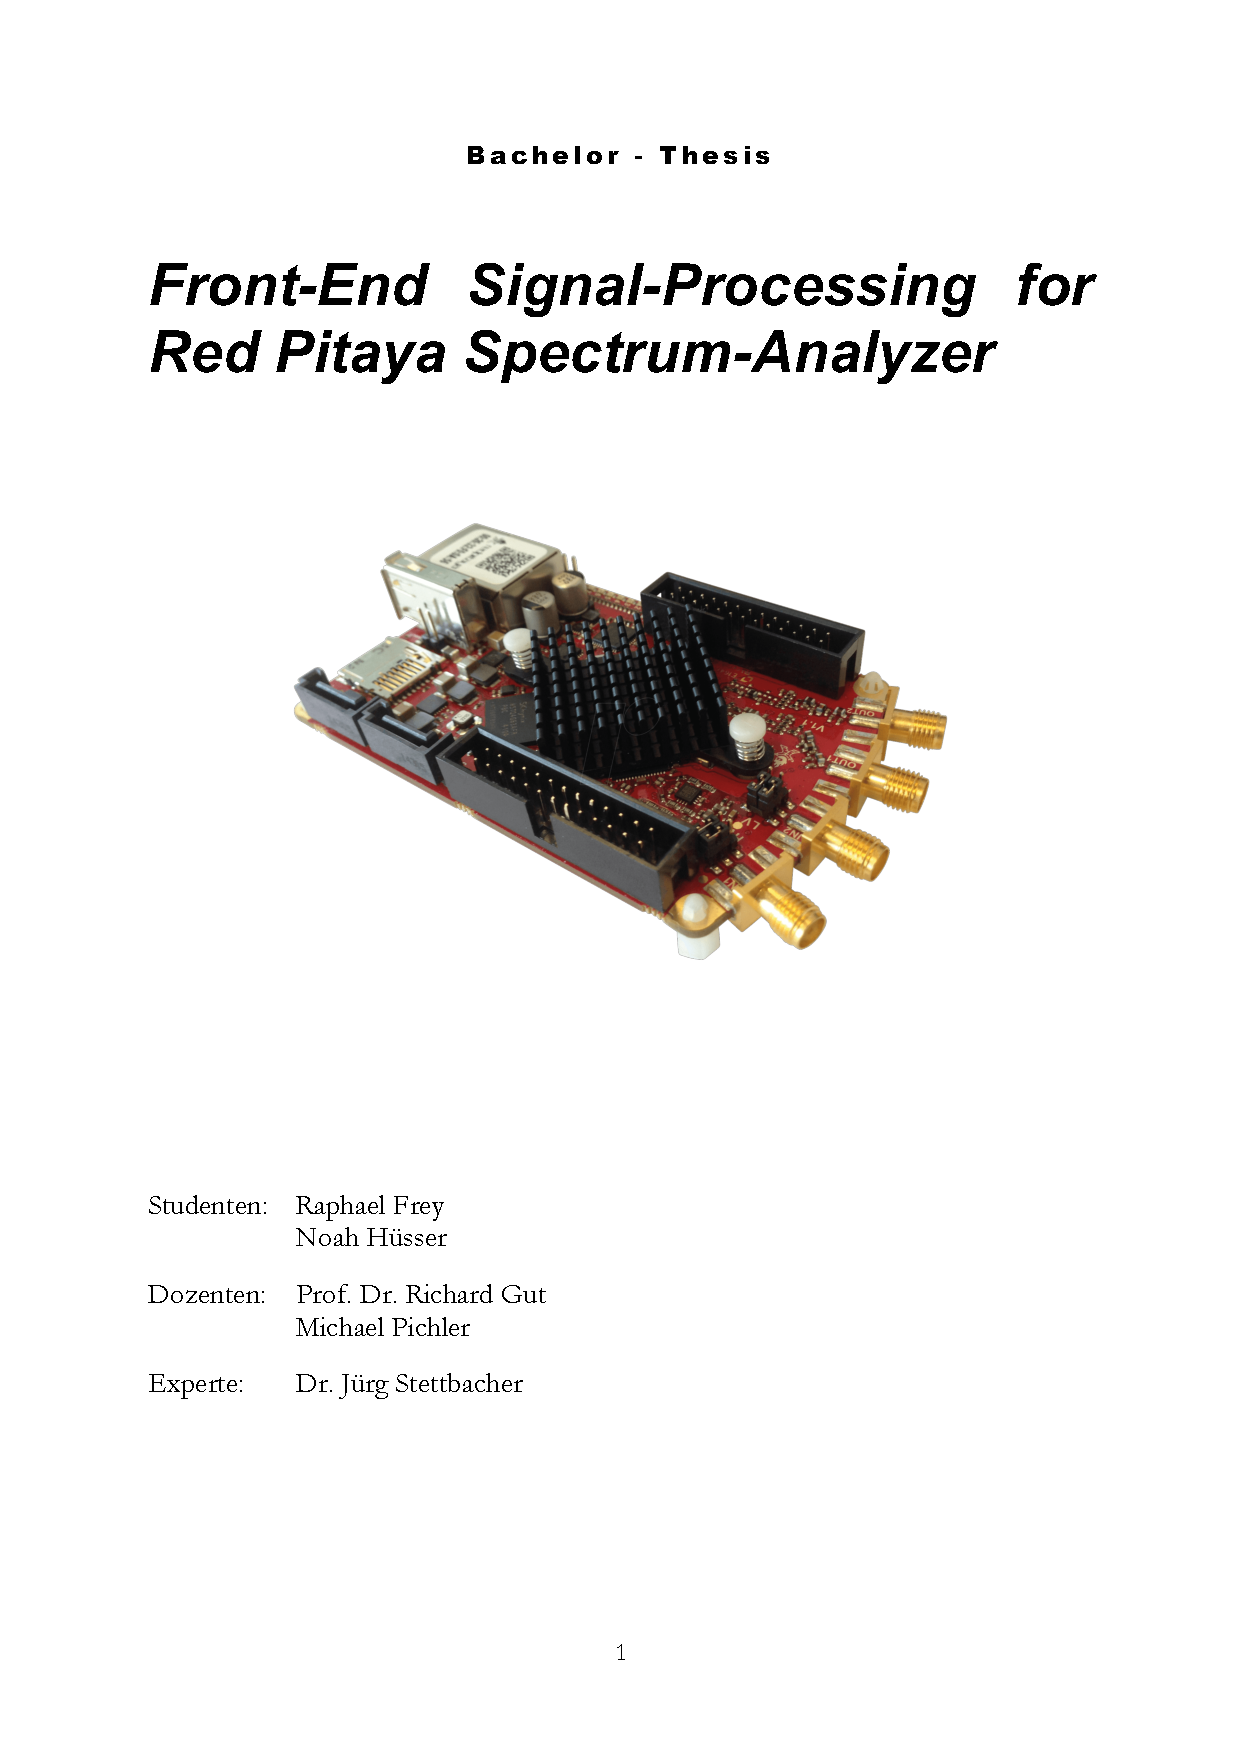
\includepdf[pages=-]{images/task.pdf}

% ==============================================================================
%
%                               P R E A M B L E
%
% ==============================================================================
\chapter{Storage Media} % --------------------------------------------------------- %
\label{ch:app:media}
% ---------------------------------------------------------------------------- %

If  you have  a physical  copy of  this report,  this appendix  may contain  a
storage medium  with a  copy of  the project  repository. A current  copy can
always be obtained by either cloning the Github repository from
\href{https://github.com/alpenwasser/pitaya/}{\nolinkurl{https://github.com/alpenwasser/pitaya/}},
or by downloading a release archive from 
\href{https://github.com/alpenwasser/pitaya/releases}{\nolinkurl{https://github.com/alpenwasser/pitaya/releases}}.


% Matlab-prettifier: Uses the lstlisting counter
% Minted: Uses the listing counter

% >>>
% ==============================================================================
%
%                             B A C K M A T T E R
%
% ==============================================================================
\cleardoublepage % <<< -------------------------------------------- BACKMATTER %
\backmatter
% Indexing: memman.pdf, pp. 302ff.
\printindex
%>>>

\end{document}
%^^A vim: foldenable foldcolumn=4 foldmethod=marker foldmarker=<<<,>>>
